% Options for packages loaded elsewhere
\PassOptionsToPackage{unicode}{hyperref}
\PassOptionsToPackage{hyphens}{url}
\PassOptionsToPackage{dvipsnames,svgnames,x11names}{xcolor}
%
\documentclass[
  letterpaper,
  DIV=11,
  numbers=noendperiod]{scrreprt}

\usepackage{amsmath,amssymb}
\usepackage{iftex}
\ifPDFTeX
  \usepackage[T1]{fontenc}
  \usepackage[utf8]{inputenc}
  \usepackage{textcomp} % provide euro and other symbols
\else % if luatex or xetex
  \usepackage{unicode-math}
  \defaultfontfeatures{Scale=MatchLowercase}
  \defaultfontfeatures[\rmfamily]{Ligatures=TeX,Scale=1}
\fi
\usepackage{lmodern}
\ifPDFTeX\else  
    % xetex/luatex font selection
\fi
% Use upquote if available, for straight quotes in verbatim environments
\IfFileExists{upquote.sty}{\usepackage{upquote}}{}
\IfFileExists{microtype.sty}{% use microtype if available
  \usepackage[]{microtype}
  \UseMicrotypeSet[protrusion]{basicmath} % disable protrusion for tt fonts
}{}
\makeatletter
\@ifundefined{KOMAClassName}{% if non-KOMA class
  \IfFileExists{parskip.sty}{%
    \usepackage{parskip}
  }{% else
    \setlength{\parindent}{0pt}
    \setlength{\parskip}{6pt plus 2pt minus 1pt}}
}{% if KOMA class
  \KOMAoptions{parskip=half}}
\makeatother
\usepackage{xcolor}
\setlength{\emergencystretch}{3em} % prevent overfull lines
\setcounter{secnumdepth}{5}
% Make \paragraph and \subparagraph free-standing
\ifx\paragraph\undefined\else
  \let\oldparagraph\paragraph
  \renewcommand{\paragraph}[1]{\oldparagraph{#1}\mbox{}}
\fi
\ifx\subparagraph\undefined\else
  \let\oldsubparagraph\subparagraph
  \renewcommand{\subparagraph}[1]{\oldsubparagraph{#1}\mbox{}}
\fi

\usepackage{color}
\usepackage{fancyvrb}
\newcommand{\VerbBar}{|}
\newcommand{\VERB}{\Verb[commandchars=\\\{\}]}
\DefineVerbatimEnvironment{Highlighting}{Verbatim}{commandchars=\\\{\}}
% Add ',fontsize=\small' for more characters per line
\usepackage{framed}
\definecolor{shadecolor}{RGB}{241,243,245}
\newenvironment{Shaded}{\begin{snugshade}}{\end{snugshade}}
\newcommand{\AlertTok}[1]{\textcolor[rgb]{0.68,0.00,0.00}{#1}}
\newcommand{\AnnotationTok}[1]{\textcolor[rgb]{0.37,0.37,0.37}{#1}}
\newcommand{\AttributeTok}[1]{\textcolor[rgb]{0.40,0.45,0.13}{#1}}
\newcommand{\BaseNTok}[1]{\textcolor[rgb]{0.68,0.00,0.00}{#1}}
\newcommand{\BuiltInTok}[1]{\textcolor[rgb]{0.00,0.23,0.31}{#1}}
\newcommand{\CharTok}[1]{\textcolor[rgb]{0.13,0.47,0.30}{#1}}
\newcommand{\CommentTok}[1]{\textcolor[rgb]{0.37,0.37,0.37}{#1}}
\newcommand{\CommentVarTok}[1]{\textcolor[rgb]{0.37,0.37,0.37}{\textit{#1}}}
\newcommand{\ConstantTok}[1]{\textcolor[rgb]{0.56,0.35,0.01}{#1}}
\newcommand{\ControlFlowTok}[1]{\textcolor[rgb]{0.00,0.23,0.31}{#1}}
\newcommand{\DataTypeTok}[1]{\textcolor[rgb]{0.68,0.00,0.00}{#1}}
\newcommand{\DecValTok}[1]{\textcolor[rgb]{0.68,0.00,0.00}{#1}}
\newcommand{\DocumentationTok}[1]{\textcolor[rgb]{0.37,0.37,0.37}{\textit{#1}}}
\newcommand{\ErrorTok}[1]{\textcolor[rgb]{0.68,0.00,0.00}{#1}}
\newcommand{\ExtensionTok}[1]{\textcolor[rgb]{0.00,0.23,0.31}{#1}}
\newcommand{\FloatTok}[1]{\textcolor[rgb]{0.68,0.00,0.00}{#1}}
\newcommand{\FunctionTok}[1]{\textcolor[rgb]{0.28,0.35,0.67}{#1}}
\newcommand{\ImportTok}[1]{\textcolor[rgb]{0.00,0.46,0.62}{#1}}
\newcommand{\InformationTok}[1]{\textcolor[rgb]{0.37,0.37,0.37}{#1}}
\newcommand{\KeywordTok}[1]{\textcolor[rgb]{0.00,0.23,0.31}{#1}}
\newcommand{\NormalTok}[1]{\textcolor[rgb]{0.00,0.23,0.31}{#1}}
\newcommand{\OperatorTok}[1]{\textcolor[rgb]{0.37,0.37,0.37}{#1}}
\newcommand{\OtherTok}[1]{\textcolor[rgb]{0.00,0.23,0.31}{#1}}
\newcommand{\PreprocessorTok}[1]{\textcolor[rgb]{0.68,0.00,0.00}{#1}}
\newcommand{\RegionMarkerTok}[1]{\textcolor[rgb]{0.00,0.23,0.31}{#1}}
\newcommand{\SpecialCharTok}[1]{\textcolor[rgb]{0.37,0.37,0.37}{#1}}
\newcommand{\SpecialStringTok}[1]{\textcolor[rgb]{0.13,0.47,0.30}{#1}}
\newcommand{\StringTok}[1]{\textcolor[rgb]{0.13,0.47,0.30}{#1}}
\newcommand{\VariableTok}[1]{\textcolor[rgb]{0.07,0.07,0.07}{#1}}
\newcommand{\VerbatimStringTok}[1]{\textcolor[rgb]{0.13,0.47,0.30}{#1}}
\newcommand{\WarningTok}[1]{\textcolor[rgb]{0.37,0.37,0.37}{\textit{#1}}}

\providecommand{\tightlist}{%
  \setlength{\itemsep}{0pt}\setlength{\parskip}{0pt}}\usepackage{longtable,booktabs,array}
\usepackage{calc} % for calculating minipage widths
% Correct order of tables after \paragraph or \subparagraph
\usepackage{etoolbox}
\makeatletter
\patchcmd\longtable{\par}{\if@noskipsec\mbox{}\fi\par}{}{}
\makeatother
% Allow footnotes in longtable head/foot
\IfFileExists{footnotehyper.sty}{\usepackage{footnotehyper}}{\usepackage{footnote}}
\makesavenoteenv{longtable}
\usepackage{graphicx}
\makeatletter
\def\maxwidth{\ifdim\Gin@nat@width>\linewidth\linewidth\else\Gin@nat@width\fi}
\def\maxheight{\ifdim\Gin@nat@height>\textheight\textheight\else\Gin@nat@height\fi}
\makeatother
% Scale images if necessary, so that they will not overflow the page
% margins by default, and it is still possible to overwrite the defaults
% using explicit options in \includegraphics[width, height, ...]{}
\setkeys{Gin}{width=\maxwidth,height=\maxheight,keepaspectratio}
% Set default figure placement to htbp
\makeatletter
\def\fps@figure{htbp}
\makeatother
\newlength{\cslhangindent}
\setlength{\cslhangindent}{1.5em}
\newlength{\csllabelwidth}
\setlength{\csllabelwidth}{3em}
\newlength{\cslentryspacingunit} % times entry-spacing
\setlength{\cslentryspacingunit}{\parskip}
\newenvironment{CSLReferences}[2] % #1 hanging-ident, #2 entry spacing
 {% don't indent paragraphs
  \setlength{\parindent}{0pt}
  % turn on hanging indent if param 1 is 1
  \ifodd #1
  \let\oldpar\par
  \def\par{\hangindent=\cslhangindent\oldpar}
  \fi
  % set entry spacing
  \setlength{\parskip}{#2\cslentryspacingunit}
 }%
 {}
\usepackage{calc}
\newcommand{\CSLBlock}[1]{#1\hfill\break}
\newcommand{\CSLLeftMargin}[1]{\parbox[t]{\csllabelwidth}{#1}}
\newcommand{\CSLRightInline}[1]{\parbox[t]{\linewidth - \csllabelwidth}{#1}\break}
\newcommand{\CSLIndent}[1]{\hspace{\cslhangindent}#1}

\usepackage{booktabs}
\usepackage{longtable}
\usepackage{array}
\usepackage{multirow}
\usepackage{wrapfig}
\usepackage{float}
\usepackage{colortbl}
\usepackage{pdflscape}
\usepackage{tabu}
\usepackage{threeparttable}
\usepackage{threeparttablex}
\usepackage[normalem]{ulem}
\usepackage{makecell}
\usepackage{xcolor}
\KOMAoption{captions}{tableheading}
\makeatletter
\makeatother
\makeatletter
\@ifpackageloaded{bookmark}{}{\usepackage{bookmark}}
\makeatother
\makeatletter
\@ifpackageloaded{caption}{}{\usepackage{caption}}
\AtBeginDocument{%
\ifdefined\contentsname
  \renewcommand*\contentsname{Table of contents}
\else
  \newcommand\contentsname{Table of contents}
\fi
\ifdefined\listfigurename
  \renewcommand*\listfigurename{List of Figures}
\else
  \newcommand\listfigurename{List of Figures}
\fi
\ifdefined\listtablename
  \renewcommand*\listtablename{List of Tables}
\else
  \newcommand\listtablename{List of Tables}
\fi
\ifdefined\figurename
  \renewcommand*\figurename{Figure}
\else
  \newcommand\figurename{Figure}
\fi
\ifdefined\tablename
  \renewcommand*\tablename{Table}
\else
  \newcommand\tablename{Table}
\fi
}
\@ifpackageloaded{float}{}{\usepackage{float}}
\floatstyle{ruled}
\@ifundefined{c@chapter}{\newfloat{codelisting}{h}{lop}}{\newfloat{codelisting}{h}{lop}[chapter]}
\floatname{codelisting}{Listing}
\newcommand*\listoflistings{\listof{codelisting}{List of Listings}}
\makeatother
\makeatletter
\@ifpackageloaded{caption}{}{\usepackage{caption}}
\@ifpackageloaded{subcaption}{}{\usepackage{subcaption}}
\makeatother
\makeatletter
\@ifpackageloaded{tcolorbox}{}{\usepackage[skins,breakable]{tcolorbox}}
\makeatother
\makeatletter
\@ifundefined{shadecolor}{\definecolor{shadecolor}{rgb}{.97, .97, .97}}
\makeatother
\makeatletter
\makeatother
\makeatletter
\makeatother
\ifLuaTeX
  \usepackage{selnolig}  % disable illegal ligatures
\fi
\IfFileExists{bookmark.sty}{\usepackage{bookmark}}{\usepackage{hyperref}}
\IfFileExists{xurl.sty}{\usepackage{xurl}}{} % add URL line breaks if available
\urlstyle{same} % disable monospaced font for URLs
\hypersetup{
  pdftitle={Comparative Effectiveness and Personalized Medicine Research Using Real-World Data},
  pdfauthor={Thomas P. A. Debray, Tri-Long Nguyen, and Robert W. Platt},
  colorlinks=true,
  linkcolor={blue},
  filecolor={Maroon},
  citecolor={Blue},
  urlcolor={Blue},
  pdfcreator={LaTeX via pandoc}}

\title{Comparative Effectiveness and Personalized Medicine Research
Using Real-World Data}
\author{Thomas Debray}
\date{2023-05-03}

\begin{document}
\maketitle
\ifdefined\Shaded\renewenvironment{Shaded}{\begin{tcolorbox}[interior hidden, sharp corners, borderline west={3pt}{0pt}{shadecolor}, boxrule=0pt, breakable, enhanced, frame hidden]}{\end{tcolorbox}}\fi

\renewcommand*\contentsname{Table of contents}
{
\hypersetup{linkcolor=}
\setcounter{tocdepth}{2}
\tableofcontents
}
\bookmarksetup{startatroot}

\hypertarget{preface}{%
\chapter{Preface}\label{preface}}

Thomas Debray (Smart Data Analysis and Statistics B.V.)

\hfill\break

\hypertarget{about-this-book}{%
\section*{About this book}\label{about-this-book}}
\addcontentsline{toc}{section}{About this book}

\markright{About this book}

This book provides practical guidance for estimating the effectiveness
of treatments in real-world populations. It explains how real-world data
can directly be used or combined with other data sources to derive
overall and individualized estimates of treatment effect. The book
explains statistical methods for implementing bias adjustments,
conducting evidence synthesis and individualizing treatment effect,
whilst also providing illustrative examples and supporting software. The
chapters and contents of the book are written by leading experts, with a
track record in the generation and/or evaluation of real-world evidence.

This book is intended as a pivotal textbook for statisticians,
epidemiologists, methodologists, regulators and/or regulatory scientists
considering, undertaking or appraising the real-world evidence of
treatment effectiveness. It covers key concepts and stages to derive and
evaluate treatment effect estimates for entire populations and specific
individuals. The book offers a conceptual framework towards estimating
treatment effects at both the population and individualized level, where
modelling methods may include traditional regression-based and machine
learning methods.

\hypertarget{motivation}{%
\section*{Motivation}\label{motivation}}
\addcontentsline{toc}{section}{Motivation}

\markright{Motivation}

Although randomized clinical trials traditionally form the cornerstone
of comparative effectiveness research, there is a growing demand to
consider evidence from ``real-world data'' (RWD) in clinical
decision-making. These data are often available from observational
cohort studies, administrative databases, and patient registries, and
may offer additional insights into the comparative effectiveness and
safety of treatments. Yet, the analysis of RWD and the evaluation of
real-world evidence face many operational and methodological challenges.

In this book, we aim to address three current needs. First, this book
will offer the guidance that is currently lacking on assessing the
quality of RWD and on implementing appropriate statistical methods to
reduce bias of single study estimates of treatment effects. Second, this
book will provide researchers with advanced approaches to pooling
estimates from multiple non-randomized studies for which traditional
evidence synthesis methods are not suitable. Finally, to answer the
growing need to translate average estimates of treatment effects to
individualized clinical decision-making, this book will present recent
methods for more tailored approaches where patient characteristics are
used to derive their individualized prognosis and treatment benefit.

This book aims to explain key principles and state-of-the-art methods
for deriving treatment effects in entire populations and specific
individuals using RWD. It will not only discuss statistical theory by
key experts in the field; it will also provide illustrative examples and
practical guidance for implementation in R. In short, the book aims to
prepare a new generation of researchers who wish to generate and
integrate evidence from both randomized and non-randomized data sources
to investigate the real-world effectiveness of treatments in populations
and individual patients.

\hypertarget{contents}{%
\section*{Contents}\label{contents}}
\addcontentsline{toc}{section}{Contents}

\markright{Contents}

The book is divided into six sections:

\begin{enumerate}
\def\labelenumi{\arabic{enumi}.}
\tightlist
\item
  \textbf{Introduction}. This section introduces the relevance of
  real-world data for conducting comparative effectiveness research, and
  discusses various concerns regarding their use.
\item
  \textbf{Principles of treatment effect estimation using real-world
  data}. In this section, we discuss key principles of treatment effect
  estimation in non-randomized data sources. We explain methods to
  adjust for confounding (including propensity score analysis and
  disease risk score analysis) and missing data when estimating the
  treatment effect for a specific (sub)population.
\item
  \textbf{Principles of evidence synthesis}. In this section, we discuss
  statistical methods for estimating the treatment effect using
  (individual participant and/or aggregate) data from multiple studies.
  To this purpose, key principles of meta-analysis are introduced and
  explained, including the standard fixed effect and random effects
  meta-analysis models, methods for individual patient data (IPD)
  meta-analysis, methods for network meta-analysis, and methods for
  data-driven and tailored bias adjustment.
\item
  \textbf{Advanced modelling issues for dealing with additional bias in
  both randomized and non-randomized data sources}. In this section, we
  discuss advanced statistical and machine learning methods for dealing
  with time-varying confounding, informative visit schedules, and
  measurement error.
\item
  \textbf{Individualizing treatment effects for personalized medicine}.
  In this section, we discuss statistical methods to estimate and
  evaluate individualized treatment effects.
\item
  Closing
\end{enumerate}

\bookmarksetup{startatroot}

\hypertarget{validity-control-and-quality-assessment-of-real-world-data-and-real-world-evidence}{%
\chapter{Validity control and quality assessment of real-world data and
real-world
evidence}\label{validity-control-and-quality-assessment-of-real-world-data-and-real-world-evidence}}

Christina ReadThomas Debray (Smart Data Analysis and Statistics B.V.)

\hfill\break

\begin{Shaded}
\begin{Highlighting}[]
\FunctionTok{library}\NormalTok{(readxl)}
\FunctionTok{library}\NormalTok{(robvis)}
\end{Highlighting}
\end{Shaded}

The quality of real-world data is often suboptimal and can therefore
lead to bias when generating real-world evidence (RWE). In this chapter,
we will introduce key quality concerns of RWD, including their accuracy,
completeness, and timeliness. Subsequently, we will discuss which steps
can be taken to assess the quality of RWD, and determine their fitness
for use. The chapter will also introduce directed acyclic graphs to
explain how the analysis of RWD may be affected by different types of
bias. We will put particular focus on confounding bias, selection bias,
and information bias, and explain how these biases can be addressed by
referring to specific chapters from the book. Finally, the chapter
presents common quality appraisal tools that can be used to assess the
quality of real-world evidence (for instance when conducting a
systematic review).

\hypertarget{example-code}{%
\section{Example code}\label{example-code}}

A risk of bias assessment was conducted in the COVID-NMA review. We can
create a summary table of risk of bias assessment and produce a traffic
light plot as follows:

\begin{Shaded}
\begin{Highlighting}[]
\NormalTok{Risk\_of\_Bias }\OtherTok{\textless{}{-}} \FunctionTok{read\_excel}\NormalTok{(}\StringTok{"resources/RoB{-}covid.xlsx"}\NormalTok{)}

\CommentTok{\#creation of traffic light plot}
\NormalTok{trafficlight\_rob }\OtherTok{\textless{}{-}} \FunctionTok{rob\_traffic\_light}\NormalTok{(}\AttributeTok{data =}\NormalTok{ Risk\_of\_Bias, }\AttributeTok{tool =} \StringTok{"ROB2"}\NormalTok{)}
\NormalTok{trafficlight\_rob}
\end{Highlighting}
\end{Shaded}

\begin{figure}[H]

{\centering 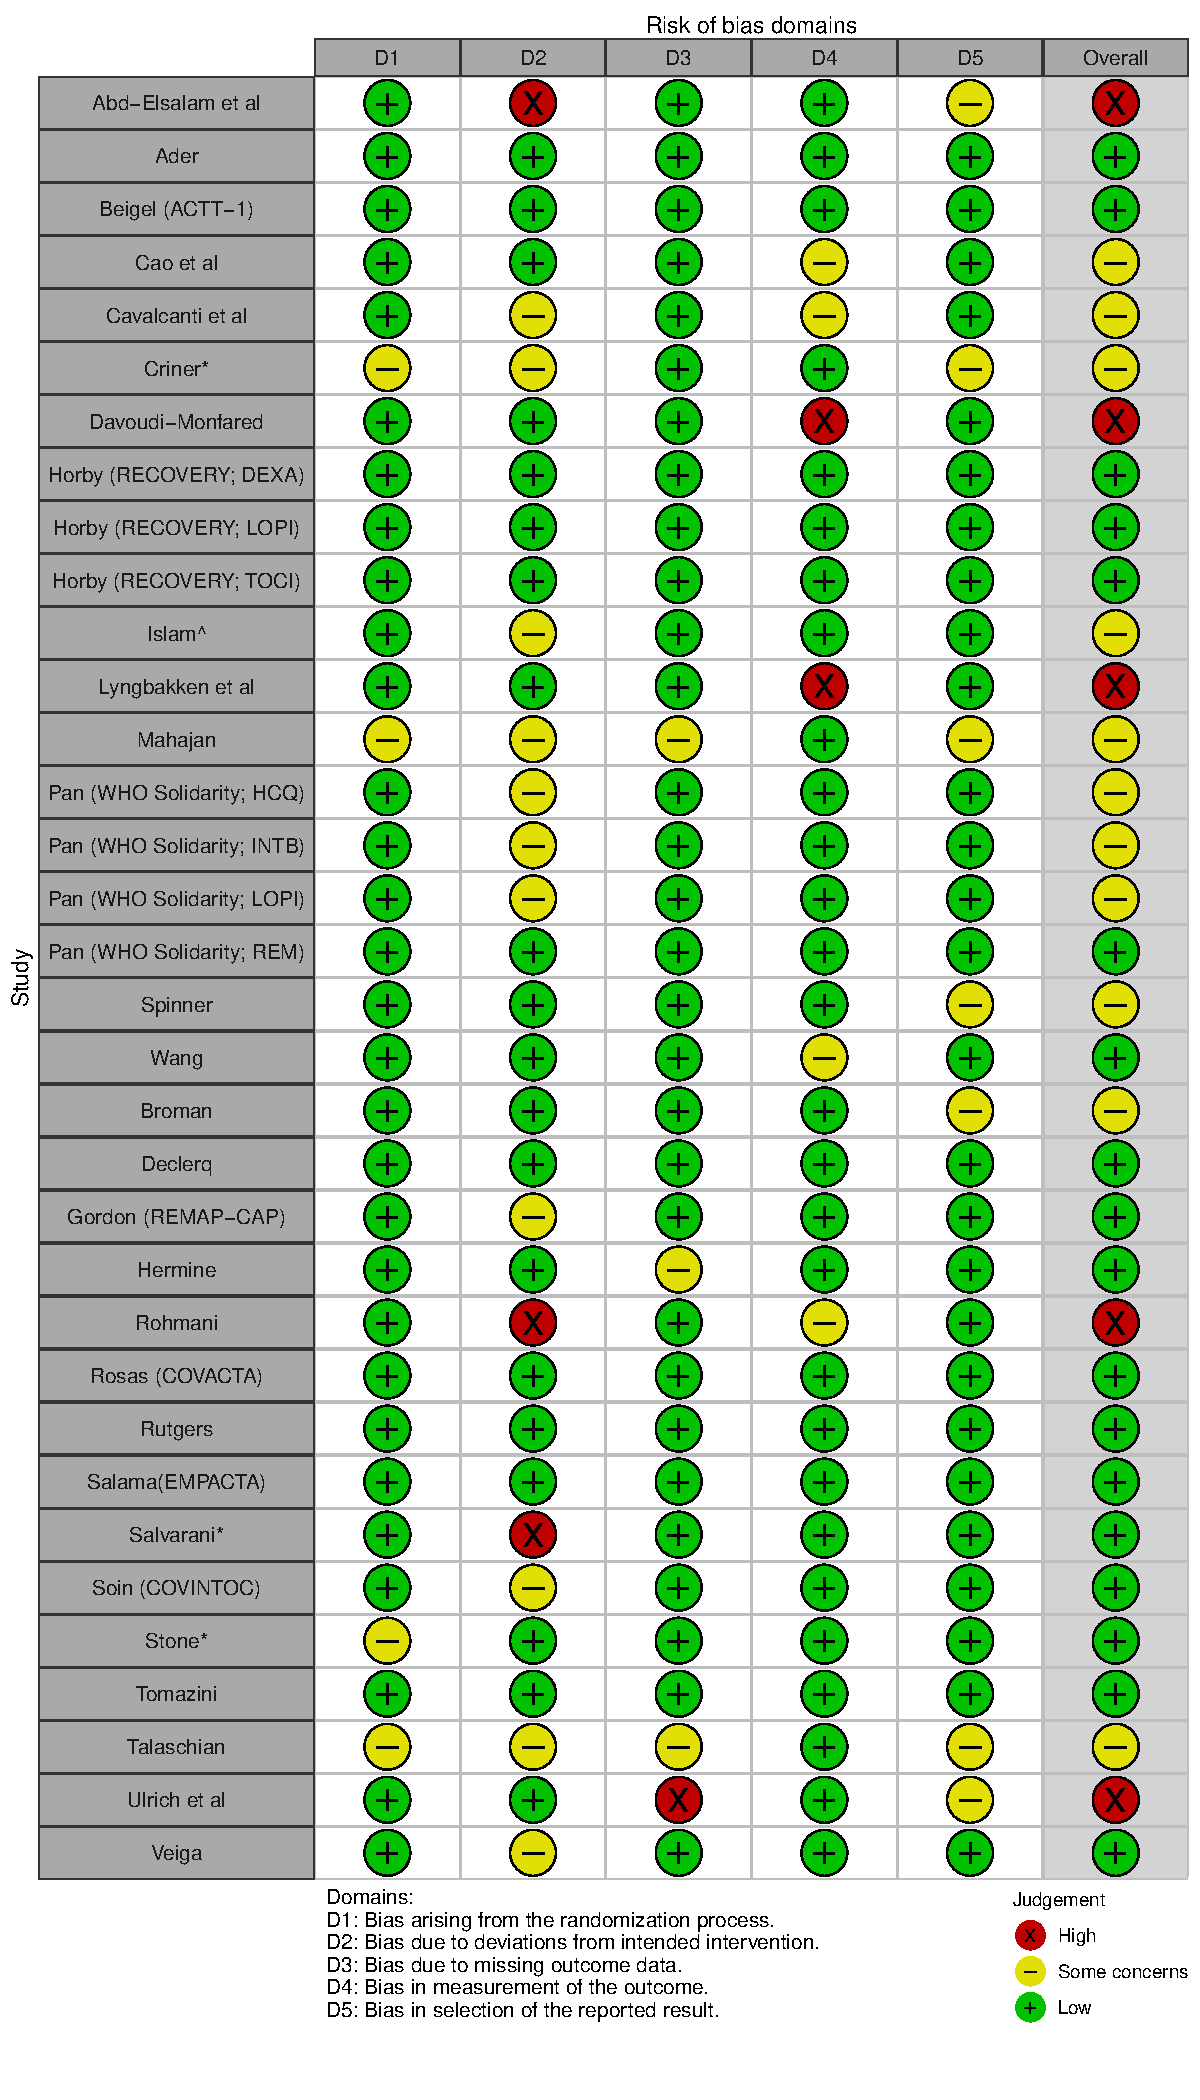
\includegraphics{chapter_03_files/figure-pdf/unnamed-chunk-2-1.pdf}

}

\end{figure}

\hypertarget{version-info}{%
\section*{Version info}\label{version-info}}
\addcontentsline{toc}{section}{Version info}

\markright{Version info}

This chapter was rendered using the following version of R and its
packages:

\begin{verbatim}
R version 4.2.3 (2023-03-15 ucrt)
Platform: x86_64-w64-mingw32/x64 (64-bit)
Running under: Windows 10 x64 (build 19045)

Matrix products: default

locale:
[1] LC_COLLATE=Dutch_Netherlands.utf8  LC_CTYPE=Dutch_Netherlands.utf8   
[3] LC_MONETARY=Dutch_Netherlands.utf8 LC_NUMERIC=C                      
[5] LC_TIME=Dutch_Netherlands.utf8    

attached base packages:
[1] stats     graphics  grDevices utils     datasets  methods   base     

other attached packages:
[1] robvis_0.3.0.900 readxl_1.4.2    

loaded via a namespace (and not attached):
 [1] cellranger_1.1.0 pillar_1.9.0     compiler_4.2.3   tools_4.2.3     
 [5] digest_0.6.31    jsonlite_1.8.5   evaluate_0.21    lifecycle_1.0.3 
 [9] tibble_3.2.1     gtable_0.3.3     pkgconfig_2.0.3  rlang_1.1.1     
[13] cli_3.6.1        rstudioapi_0.14  yaml_2.3.7       xfun_0.39       
[17] fastmap_1.1.1    withr_2.5.0      stringr_1.5.0    dplyr_1.1.2     
[21] knitr_1.43       generics_0.1.3   vctrs_0.6.3      grid_4.2.3      
[25] tidyselect_1.2.0 glue_1.6.2       R6_2.5.1         fansi_1.0.4     
[29] rmarkdown_2.22   farver_2.1.1     tidyr_1.3.0      purrr_1.0.1     
[33] ggplot2_3.4.2    magrittr_2.0.3   scales_1.2.1     codetools_0.2-19
[37] htmltools_0.5.5  colorspace_2.1-0 utf8_1.2.3       stringi_1.7.12  
[41] munsell_0.5.0   
\end{verbatim}

\bookmarksetup{startatroot}

\hypertarget{confounding-adjustment-using-propensity-score-methods}{%
\chapter{Confounding adjustment using propensity score
methods}\label{confounding-adjustment-using-propensity-score-methods}}

Tammy Jiang (Biogen)\\
Thomas Debray (Smart Data Analysis and Statistics B.V.)

\hfill\break

\hypertarget{introduction}{%
\section{Introduction}\label{introduction}}

The purpose of this document is to provide example R code that
demonstrates how to estimate the propensity score and implement
matching, stratification, weighting, and regression adjustment for the
continuous propensity score. In this example using simulated data, we
have two disease modifying therapies (DMT1 and DMT0) and the outcome is
the number of post-treatment multiple sclerosis relapses during
follow-up. We will estimate the average treatment effect in the treated
(ATT) using propensity score matching, stratification, and weighting. We
will estimate the average treatment effect in the population (ATE) using
regression adjustment for the continuous propensity score. The treatment
effects can be interpreted as annualized relapse rate ratios (ARR).

We consider an example dataset with the following characteristics:

\begin{Shaded}
\begin{Highlighting}[]
\FunctionTok{head}\NormalTok{(dat)}
\end{Highlighting}
\end{Shaded}

\begin{verbatim}
   age female prevDMTefficacy premedicalcost numSymptoms prerelapse_num
1:  50      1            None        3899.61           1              1
2:  51      0            None        9580.51           1              0
3:  56      0            None        4785.89           1              0
4:  44      1            None        8696.80           1              1
5:  63      0            None        2588.03           1              0
6:  28      1            None        5435.57           1              0
   treatment y      years      Iscore
1:      DMT1 0 1.78507871 Moderate A1
2:      DMT1 0 0.01368925     High A1
3:      DMT1 2 3.25530459     High A1
4:      DMT1 2 5.73853525     Neutral
5:      DMT1 0 1.31143053     High A1
6:      DMT1 0 0.59137577 Moderate A0
\end{verbatim}

\hypertarget{comparing-baseline-characteristics}{%
\section{Comparing baseline
characteristics}\label{comparing-baseline-characteristics}}

\begin{itemize}
\tightlist
\item
  \texttt{DMT1} is the treatment group and \texttt{DMT0} is the control
  group
\item
  \texttt{prevDMTefficacy} is previous DMT efficacy (none, low efficacy,
  and medium/high efficacy)
\item
  \texttt{prerelapse\_num} is the number of previous MS relapses
\end{itemize}

\begin{longtable}[]{@{}lll@{}}
\toprule\noalign{}
& DMT0 & DMT1 \\
\midrule\noalign{}
\endhead
\bottomrule\noalign{}
\endlastfoot
n & 2300 & 7700 \\
age (mean (SD)) & 51.39 (8.32) & 44.25 (9.79) \\
female = 1 (\%) & 1671 (72.65) & 5915 (76.82) \\
prevDMTefficacy (\%) & & \\
None & 1247 (54.22) & 3171 (41.18) \\
Low\_efficacy & 261 (11.35) & 858 (11.14) \\
Medium\_high\_efficacy & 792 (34.43) & 3671 (47.68) \\
prerelapse\_num (mean (SD)) & 0.39 (0.62) & 0.46 (0.68) \\
\end{longtable}

\hypertarget{estimating-the-propensity-score}{%
\section{Estimating the propensity
score}\label{estimating-the-propensity-score}}

\hypertarget{logistic-regression}{%
\subsection{Logistic regression}\label{logistic-regression}}

We sought to restore balance in the distribution of baseline covariates
in patients treated with DMT1 (index treatment) and DMT0 (control
tratment). We fit a multivariable logistic regression model in which
treatment was regressed on baseline characteristics including age, sex,
previous DMT efficacy, and previous number of relapses.

\begin{Shaded}
\begin{Highlighting}[]
\CommentTok{\# Fit logistic regression model}
\NormalTok{ps.model }\OtherTok{\textless{}{-}} \FunctionTok{glm}\NormalTok{(treatment }\SpecialCharTok{\textasciitilde{}}\NormalTok{ age }\SpecialCharTok{+}\NormalTok{ female }\SpecialCharTok{+}\NormalTok{ prevDMTefficacy }\SpecialCharTok{+}\NormalTok{ prerelapse\_num, }
                \AttributeTok{data =}\NormalTok{ dat, }\AttributeTok{family =} \FunctionTok{binomial}\NormalTok{())}

\CommentTok{\# Summary of logistic regression model}
\FunctionTok{summary}\NormalTok{(ps.model)}
\end{Highlighting}
\end{Shaded}

\begin{verbatim}

Call:
glm(formula = treatment ~ age + female + prevDMTefficacy + prerelapse_num, 
    family = binomial(), data = dat)

Deviance Residuals: 
    Min       1Q   Median       3Q      Max  
-2.7949   0.2585   0.5220   0.7478   1.5033  

Coefficients:
                                     Estimate Std. Error z value Pr(>|z|)    
(Intercept)                          4.809473   0.157127  30.609  < 2e-16 ***
age                                 -0.086708   0.002996 -28.939  < 2e-16 ***
female1                              0.253611   0.057664   4.398 1.09e-05 ***
prevDMTefficacyLow_efficacy          0.310394   0.083022   3.739 0.000185 ***
prevDMTefficacyMedium_high_efficacy  0.660266   0.054393  12.139  < 2e-16 ***
prerelapse_num                       0.156318   0.039288   3.979 6.93e-05 ***
---
Signif. codes:  0 '***' 0.001 '**' 0.01 '*' 0.05 '.' 0.1 ' ' 1

(Dispersion parameter for binomial family taken to be 1)

    Null deviance: 10786  on 9999  degrees of freedom
Residual deviance:  9597  on 9994  degrees of freedom
AIC: 9609

Number of Fisher Scoring iterations: 5
\end{verbatim}

\begin{Shaded}
\begin{Highlighting}[]
\CommentTok{\# Extract propensity scores}
\NormalTok{dat}\SpecialCharTok{$}\NormalTok{ps }\OtherTok{\textless{}{-}} \FunctionTok{predict}\NormalTok{(ps.model, }\AttributeTok{data =}\NormalTok{ dat, }\AttributeTok{type =} \StringTok{"response"}\NormalTok{)}
\end{Highlighting}
\end{Shaded}

\hypertarget{assessing-overlap}{%
\subsection{Assessing overlap}\label{assessing-overlap}}

We examined the degree of overlap in the distribution of propensity
scores across treatment groups using histograms and side-by-side box
plots.

\begin{Shaded}
\begin{Highlighting}[]
\CommentTok{\# Histogram}
\FunctionTok{ggplot}\NormalTok{(dat, }\FunctionTok{aes}\NormalTok{(}\AttributeTok{x =}\NormalTok{ ps, }\AttributeTok{fill =} \FunctionTok{as.factor}\NormalTok{(treatment), }\AttributeTok{color =} \FunctionTok{as.factor}\NormalTok{(treatment))) }\SpecialCharTok{+} 
  \FunctionTok{geom\_histogram}\NormalTok{(}\AttributeTok{alpha =} \FloatTok{0.3}\NormalTok{, }\AttributeTok{position=}\StringTok{\textquotesingle{}identity\textquotesingle{}}\NormalTok{, }\AttributeTok{bins =} \DecValTok{15}\NormalTok{) }\SpecialCharTok{+} 
  \FunctionTok{facet\_grid}\NormalTok{(}\FunctionTok{as.factor}\NormalTok{(treatment) }\SpecialCharTok{\textasciitilde{}}\NormalTok{ .) }\SpecialCharTok{+} 
  \FunctionTok{xlab}\NormalTok{(}\StringTok{"Probability of Treatment"}\NormalTok{) }\SpecialCharTok{+} 
  \FunctionTok{ylab}\NormalTok{(}\StringTok{"Count"}\NormalTok{) }\SpecialCharTok{+}
  \FunctionTok{ggtitle}\NormalTok{(}\StringTok{"Propensity Score Distribution by Treatment Group"}\NormalTok{) }\SpecialCharTok{+}
  \FunctionTok{theme}\NormalTok{(}\AttributeTok{legend.position =} \StringTok{"bottom"}\NormalTok{, }\AttributeTok{legend.direction =} \StringTok{"vertical"}\NormalTok{)}
\end{Highlighting}
\end{Shaded}

\begin{figure}[H]

{\centering 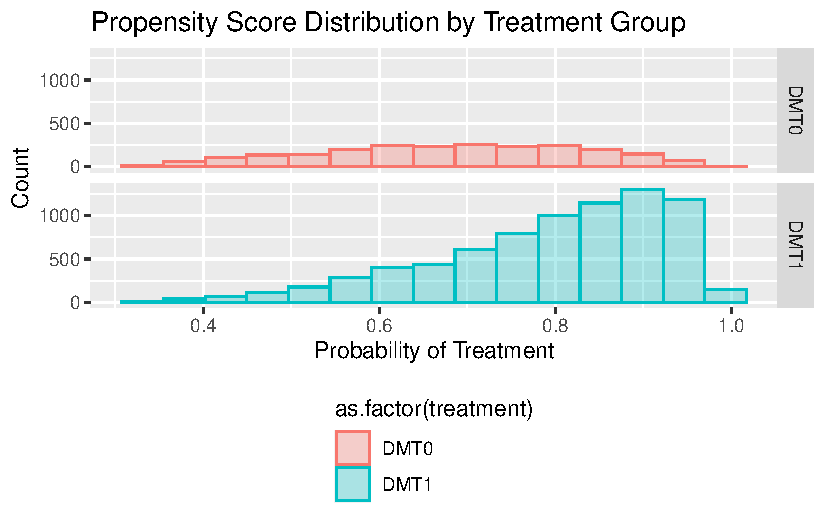
\includegraphics{chapter_06_files/figure-pdf/unnamed-chunk-8-1.pdf}

}

\end{figure}

\begin{Shaded}
\begin{Highlighting}[]
\CommentTok{\# Side{-}by{-}side box plots}
\FunctionTok{ggplot}\NormalTok{(dat, }\FunctionTok{aes}\NormalTok{(}\AttributeTok{x=}\FunctionTok{as.factor}\NormalTok{(treatment), }\AttributeTok{y=}\NormalTok{ps, }\AttributeTok{fill=}\FunctionTok{as.factor}\NormalTok{(treatment))) }\SpecialCharTok{+}
  \FunctionTok{geom\_boxplot}\NormalTok{() }\SpecialCharTok{+} 
  \FunctionTok{ggtitle}\NormalTok{(}\StringTok{"Propensity Score Distribution by Treatment Group"}\NormalTok{) }\SpecialCharTok{+}
  \FunctionTok{ylab}\NormalTok{(}\StringTok{"Probability of Treatment"}\NormalTok{) }\SpecialCharTok{+} 
  \FunctionTok{xlab}\NormalTok{(}\StringTok{"Treatment group"}\NormalTok{) }\SpecialCharTok{+}
  \FunctionTok{theme}\NormalTok{(}\AttributeTok{legend.position =} \StringTok{"none"}\NormalTok{)}
\end{Highlighting}
\end{Shaded}

\begin{figure}[H]

{\centering 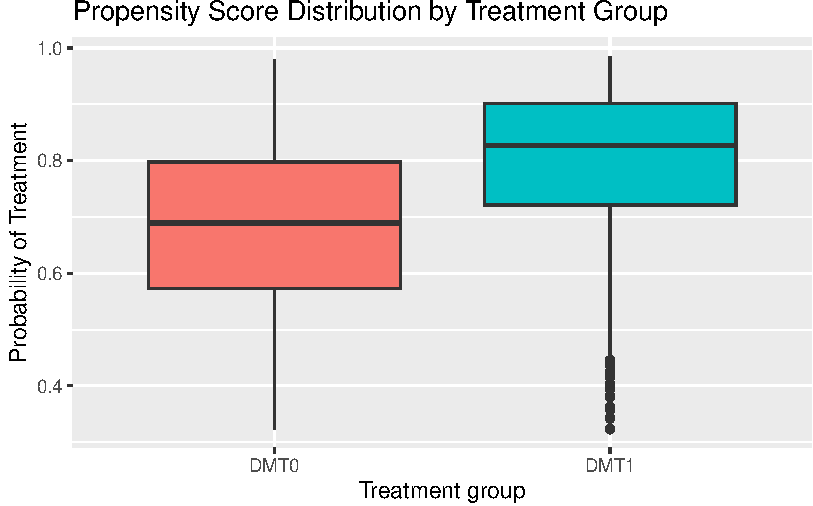
\includegraphics{chapter_06_files/figure-pdf/unnamed-chunk-8-2.pdf}

}

\end{figure}

\begin{Shaded}
\begin{Highlighting}[]
\CommentTok{\# Distribution of propensity scores by treatment groups}
\FunctionTok{summary}\NormalTok{(dat}\SpecialCharTok{$}\NormalTok{ps[dat}\SpecialCharTok{$}\NormalTok{treatment }\SpecialCharTok{==} \StringTok{"DMT1"}\NormalTok{])}
\end{Highlighting}
\end{Shaded}

\begin{verbatim}
   Min. 1st Qu.  Median    Mean 3rd Qu.    Max. 
 0.3230  0.7214  0.8265  0.7970  0.9010  0.9854 
\end{verbatim}

\begin{Shaded}
\begin{Highlighting}[]
\FunctionTok{summary}\NormalTok{(dat}\SpecialCharTok{$}\NormalTok{ps[dat}\SpecialCharTok{$}\NormalTok{treatment }\SpecialCharTok{==} \StringTok{"DMT0"}\NormalTok{])}
\end{Highlighting}
\end{Shaded}

\begin{verbatim}
   Min. 1st Qu.  Median    Mean 3rd Qu.    Max. 
 0.3230  0.5730  0.6894  0.6795  0.7975  0.9799 
\end{verbatim}

\hypertarget{propensity-score-matching}{%
\section{Propensity score matching}\label{propensity-score-matching}}

\hypertarget{optimal-full-matching-without-replacement}{%
\subsection{1:1 Optimal full matching without
replacement}\label{optimal-full-matching-without-replacement}}

\begin{Shaded}
\begin{Highlighting}[]
\FunctionTok{library}\NormalTok{(MatchIt)}

\CommentTok{\# Use MatchIt package for PS matching}
\NormalTok{opt }\OtherTok{\textless{}{-}} \FunctionTok{matchit}\NormalTok{(treatment }\SpecialCharTok{\textasciitilde{}}\NormalTok{ age }\SpecialCharTok{+}\NormalTok{ female }\SpecialCharTok{+}\NormalTok{ prevDMTefficacy }\SpecialCharTok{+}\NormalTok{ prerelapse\_num, }
               \AttributeTok{data =}\NormalTok{ dat, }
               \AttributeTok{method =} \StringTok{"full"}\NormalTok{,}
               \AttributeTok{estimand =} \StringTok{"ATT"}\NormalTok{)}

\NormalTok{opt}
\end{Highlighting}
\end{Shaded}

\begin{verbatim}
A matchit object
 - method: Optimal full matching
 - distance: Propensity score
             - estimated with logistic regression
 - number of obs.: 10000 (original), 10000 (matched)
 - target estimand: ATT
 - covariates: age, female, prevDMTefficacy, prerelapse_num
\end{verbatim}

\hypertarget{assess-balance-after-matching}{%
\subsection{Assess balance after
matching}\label{assess-balance-after-matching}}

\begin{Shaded}
\begin{Highlighting}[]
\FunctionTok{summary}\NormalTok{(opt)}
\end{Highlighting}
\end{Shaded}

\begin{verbatim}

Call:
matchit(formula = treatment ~ age + female + prevDMTefficacy + 
    prerelapse_num, data = dat, method = "full", estimand = "ATT")

Summary of Balance for All Data:
                                    Means Treated Means Control Std. Mean Diff.
distance                                   0.7970        0.6795          0.8943
age                                       44.2496       51.3883         -0.7289
female0                                    0.2318        0.2735         -0.0987
female1                                    0.7682        0.7265          0.0987
prevDMTefficacyNone                        0.4118        0.5422         -0.2649
prevDMTefficacyLow_efficacy                0.1114        0.1135         -0.0065
prevDMTefficacyMedium_high_efficacy        0.4768        0.3443          0.2651
prerelapse_num                             0.4595        0.3930          0.0976
                                    Var. Ratio eCDF Mean eCDF Max
distance                                0.7873    0.1917   0.3379
age                                     1.3868    0.1519   0.3085
female0                                      .    0.0417   0.0417
female1                                      .    0.0417   0.0417
prevDMTefficacyNone                          .    0.1304   0.1304
prevDMTefficacyLow_efficacy                  .    0.0020   0.0020
prevDMTefficacyMedium_high_efficacy          .    0.1324   0.1324
prerelapse_num                          1.1990    0.0133   0.0383

Summary of Balance for Matched Data:
                                    Means Treated Means Control Std. Mean Diff.
distance                                   0.7970        0.7970          0.0003
age                                       44.2496       44.3185         -0.0070
female0                                    0.2318        0.2275          0.0101
female1                                    0.7682        0.7725         -0.0101
prevDMTefficacyNone                        0.4118        0.4130         -0.0024
prevDMTefficacyLow_efficacy                0.1114        0.0893          0.0703
prevDMTefficacyMedium_high_efficacy        0.4768        0.4977         -0.0419
prerelapse_num                             0.4595        0.4399          0.0288
                                    Var. Ratio eCDF Mean eCDF Max
distance                                0.9976    0.0005   0.0075
age                                     1.0392    0.0038   0.0153
female0                                      .    0.0043   0.0043
female1                                      .    0.0043   0.0043
prevDMTefficacyNone                          .    0.0012   0.0012
prevDMTefficacyLow_efficacy                  .    0.0221   0.0221
prevDMTefficacyMedium_high_efficacy          .    0.0209   0.0209
prerelapse_num                          1.1319    0.0060   0.0229
                                    Std. Pair Dist.
distance                                     0.0008
age                                          0.0667
female0                                      0.1775
female1                                      0.1775
prevDMTefficacyNone                          0.1100
prevDMTefficacyLow_efficacy                  0.1846
prevDMTefficacyMedium_high_efficacy          0.1614
prerelapse_num                               0.2170

Sample Sizes:
              Control Treated
All           2300.      7700
Matched (ESS)  307.06    7700
Matched       2300.      7700
Unmatched        0.         0
Discarded        0.         0
\end{verbatim}

\begin{Shaded}
\begin{Highlighting}[]
\FunctionTok{plot}\NormalTok{(}\FunctionTok{summary}\NormalTok{(opt))}
\end{Highlighting}
\end{Shaded}

\begin{figure}[H]

{\centering 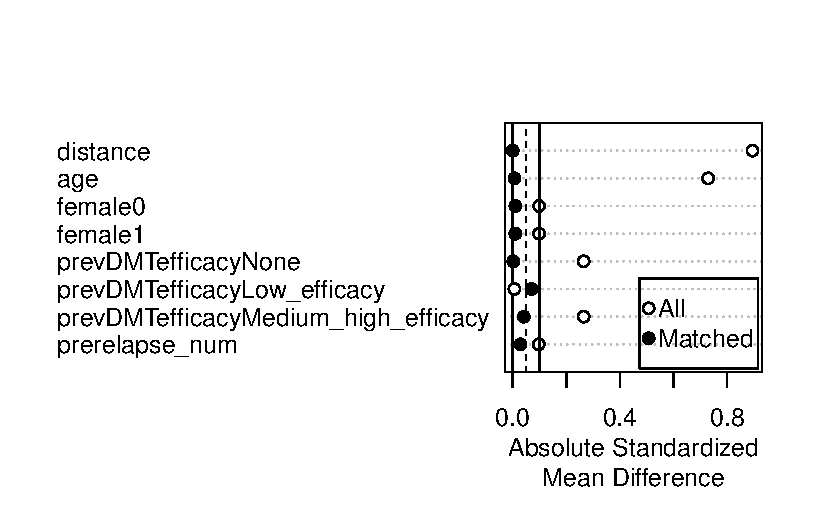
\includegraphics{chapter_06_files/figure-pdf/unnamed-chunk-11-1.pdf}

}

\end{figure}

\begin{Shaded}
\begin{Highlighting}[]
\CommentTok{\# black line is treated group, grey line is control group}
\FunctionTok{plot}\NormalTok{(opt, }\AttributeTok{type =} \StringTok{"density"}\NormalTok{, }\AttributeTok{which.xs =}\NormalTok{ vars) }
\end{Highlighting}
\end{Shaded}

\begin{figure}[H]

{\centering 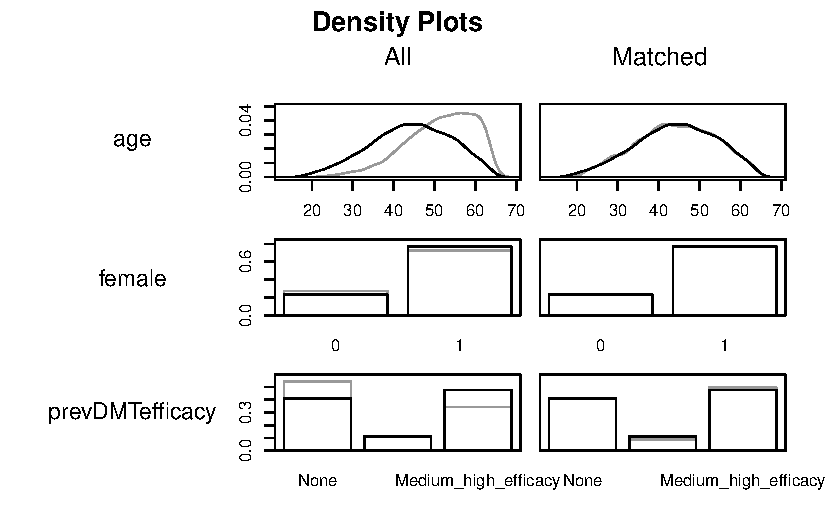
\includegraphics{chapter_06_files/figure-pdf/unnamed-chunk-11-2.pdf}

}

\end{figure}

\begin{figure}[H]

{\centering 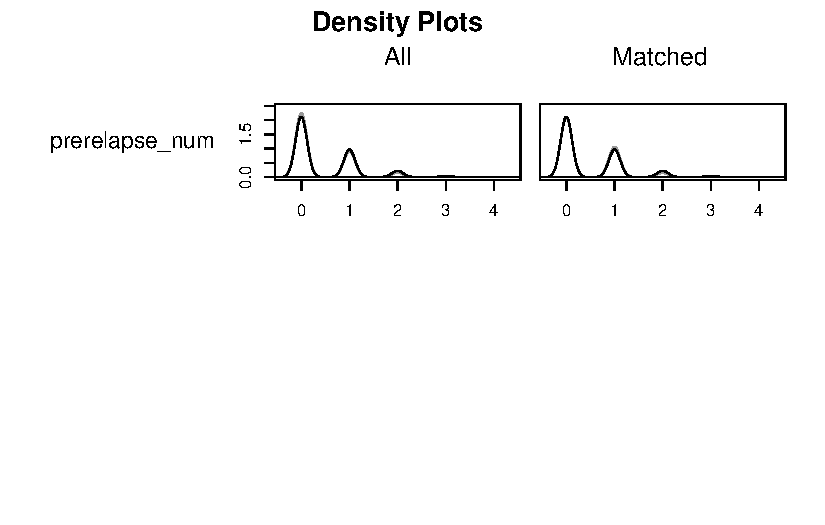
\includegraphics{chapter_06_files/figure-pdf/unnamed-chunk-11-3.pdf}

}

\end{figure}

\hypertarget{estimating-the-att}{%
\subsection{Estimating the ATT}\label{estimating-the-att}}

We can estimate the ATT in the matched sample using Poisson regression
in which the number of post-treatment relapses is regressed on treatment
status and follow-up time for each patient (captured by the variable
\texttt{years}). More details are provided at
\url{https://cran.r-project.org/web/packages/MatchIt/vignettes/estimating-effects.html}.

\begin{Shaded}
\begin{Highlighting}[]
\CommentTok{\# Matched data}
\NormalTok{matched.data }\OtherTok{\textless{}{-}} \FunctionTok{match.data}\NormalTok{(opt)}

\CommentTok{\# Poisson regression model}
\NormalTok{opt.fit }\OtherTok{\textless{}{-}} \FunctionTok{glm}\NormalTok{(y }\SpecialCharTok{\textasciitilde{}}\NormalTok{ treatment }\SpecialCharTok{+} \FunctionTok{offset}\NormalTok{(}\FunctionTok{log}\NormalTok{(years)), }
            \AttributeTok{family =} \FunctionTok{poisson}\NormalTok{(}\AttributeTok{link =} \StringTok{"log"}\NormalTok{),}
            \AttributeTok{data =}\NormalTok{ matched.data, }
            \AttributeTok{weights =}\NormalTok{ weights)}

\CommentTok{\# Treatment effect estimation}
\NormalTok{opt.comp }\OtherTok{\textless{}{-}} \FunctionTok{comparisons}\NormalTok{(opt.fit,}
                        \AttributeTok{variables =} \StringTok{"treatment"}\NormalTok{,}
                        \AttributeTok{vcov =} \SpecialCharTok{\textasciitilde{}}\NormalTok{subclass,}
                        \AttributeTok{newdata =} \FunctionTok{subset}\NormalTok{(matched.data, treatment }\SpecialCharTok{==} \StringTok{"DMT1"}\NormalTok{),}
                        \AttributeTok{wts =} \StringTok{"weights"}\NormalTok{,}
                        \AttributeTok{transform\_pre =} \StringTok{"ratio"}\NormalTok{)}

\NormalTok{opt.comp }\SpecialCharTok{|\textgreater{}} \FunctionTok{tidy}\NormalTok{()}
\end{Highlighting}
\end{Shaded}

\begin{verbatim}
# A tibble: 1 x 8
  term      contrast    estimate std.error statistic  p.value conf.low conf.high
  <chr>     <chr>          <dbl>     <dbl>     <dbl>    <dbl>    <dbl>     <dbl>
1 treatment mean(DMT1)~    0.804     0.102      7.88 3.25e-15    0.604      1.00
\end{verbatim}

As indicated in the summary output above, the annualized relapse rate
ratio for DMT1 vs DMT0 among patients treated with DMT0 (ATT) is given
as 0.8 with a 95\% confidence interval ranging from 0.6 to 1.

\hypertarget{propensity-score-stratification}{%
\section{Propensity score
stratification}\label{propensity-score-stratification}}

\hypertarget{divide-sample-into-quintiles-of-propensity-scores}{%
\subsection{Divide sample into quintiles of propensity
scores}\label{divide-sample-into-quintiles-of-propensity-scores}}

We will form five mutually exclusive groups of the estimated propensity
score.

\begin{Shaded}
\begin{Highlighting}[]
\CommentTok{\# Create five strata}
\NormalTok{dat }\OtherTok{\textless{}{-}}\NormalTok{ dat }\SpecialCharTok{\%\textgreater{}\%} \FunctionTok{mutate}\NormalTok{(}\AttributeTok{ps.strata =} \FunctionTok{cut}\NormalTok{(ps, }
                                      \AttributeTok{breaks =} \FunctionTok{c}\NormalTok{(}\FunctionTok{quantile}\NormalTok{(ps, }\AttributeTok{probs=}\FunctionTok{seq}\NormalTok{(}\DecValTok{0}\NormalTok{,}\DecValTok{1}\NormalTok{,}\FloatTok{0.2}\NormalTok{))),}
                                      \AttributeTok{labels =} \FunctionTok{seq}\NormalTok{(}\DecValTok{1}\SpecialCharTok{:}\DecValTok{5}\NormalTok{),}
                                      \AttributeTok{include.lowest =} \ConstantTok{TRUE}\NormalTok{))}

\CommentTok{\# Number of patients in each stratum}
\FunctionTok{table}\NormalTok{(dat}\SpecialCharTok{$}\NormalTok{ps.strata)}
\end{Highlighting}
\end{Shaded}

\begin{verbatim}

   1    2    3    4    5 
2002 2015 1991 1997 1995 
\end{verbatim}

\hypertarget{assess-balance-within-each-propensity-score-stratum}{%
\subsection{Assess balance within each propensity score
stratum}\label{assess-balance-within-each-propensity-score-stratum}}

Within each propensity score stratum, treated and control patients
should have similar values of the propensity score and the distribution
of baseline covariates should be approximately balanced between
treatment groups.

\hypertarget{propensity-score-stratum-1}{%
\subsubsection{Propensity Score Stratum
\#1}\label{propensity-score-stratum-1}}

\begin{Shaded}
\begin{Highlighting}[]
\NormalTok{tab1.strata1 }\OtherTok{\textless{}{-}} \FunctionTok{CreateTableOne}\NormalTok{(vars, }\AttributeTok{data =}\NormalTok{ dat }\SpecialCharTok{\%\textgreater{}\%} \FunctionTok{filter}\NormalTok{(ps.strata }\SpecialCharTok{==} \DecValTok{1}\NormalTok{), }
                               \AttributeTok{factorVars =} \FunctionTok{c}\NormalTok{(}\StringTok{"female"}\NormalTok{, }\StringTok{"prevDMTefficacy"}\NormalTok{), }
                               \AttributeTok{strata =} \StringTok{"treatment"}\NormalTok{, }\AttributeTok{test =} \ConstantTok{FALSE}\NormalTok{)}

\NormalTok{tab1.strata1.print }\OtherTok{\textless{}{-}} \FunctionTok{print}\NormalTok{(tab1.strata1, }\AttributeTok{catDigits =} \DecValTok{2}\NormalTok{, }\AttributeTok{contDigits =} \DecValTok{2}\NormalTok{, }
                            \AttributeTok{smd =} \ConstantTok{TRUE}\NormalTok{)}
\end{Highlighting}
\end{Shaded}

\begin{longtable}[]{@{}llll@{}}
\toprule\noalign{}
& DMT0 & DMT1 & SMD \\
\midrule\noalign{}
\endhead
\bottomrule\noalign{}
\endlastfoot
n & 901 & 1101 & \\
age (mean (SD)) & 58.38 (3.67) & 57.45 (3.73) & 0.251 \\
female = 1 (\%) & 605 (67.15) & 775 (70.39) & 0.070 \\
prevDMTefficacy (\%) & & & 0.056 \\
None & 650 (72.14) & 771 (70.03) & \\
Low\_efficacy & 106 (11.76) & 130 (11.81) & \\
Medium\_high\_efficacy & 145 (16.09) & 200 (18.17) & \\
prerelapse\_num (mean (SD)) & 0.29 (0.53) & 0.33 (0.56) & 0.074 \\
\end{longtable}

\hypertarget{propensity-score-stratum-2}{%
\subsubsection{Propensity Score Stratum
\#2}\label{propensity-score-stratum-2}}

\begin{Shaded}
\begin{Highlighting}[]
\NormalTok{tab1.strata2 }\OtherTok{\textless{}{-}} \FunctionTok{CreateTableOne}\NormalTok{(vars, }\AttributeTok{data =}\NormalTok{ dat }\SpecialCharTok{\%\textgreater{}\%} \FunctionTok{filter}\NormalTok{(ps.strata }\SpecialCharTok{==} \DecValTok{2}\NormalTok{), }
                               \AttributeTok{factorVars =} \FunctionTok{c}\NormalTok{(}\StringTok{"female"}\NormalTok{, }\StringTok{"prevDMTefficacy"}\NormalTok{), }
                               \AttributeTok{strata =} \StringTok{"treatment"}\NormalTok{, }\AttributeTok{test =} \ConstantTok{FALSE}\NormalTok{)}

\NormalTok{tab1.strata2.print }\OtherTok{\textless{}{-}} \FunctionTok{print}\NormalTok{(tab1.strata2, }\AttributeTok{catDigits =} \DecValTok{2}\NormalTok{, }\AttributeTok{contDigits =} \DecValTok{2}\NormalTok{, }
                            \AttributeTok{smd =} \ConstantTok{TRUE}\NormalTok{)}
\end{Highlighting}
\end{Shaded}

\begin{longtable}[]{@{}llll@{}}
\toprule\noalign{}
& DMT0 & DMT1 & SMD \\
\midrule\noalign{}
\endhead
\bottomrule\noalign{}
\endlastfoot
n & 617 & 1398 & \\
age (mean (SD)) & 52.18 (4.35) & 51.97 (4.22) & 0.049 \\
female = 1 (\%) & 458 (74.23) & 1048 (74.96) & 0.017 \\
prevDMTefficacy (\%) & & & 0.054 \\
None & 292 (47.33) & 624 (44.64) & \\
Low\_efficacy & 69 (11.18) & 162 (11.59) & \\
Medium\_high\_efficacy & 256 (41.49) & 612 (43.78) & \\
prerelapse\_num (mean (SD)) & 0.40 (0.64) & 0.41 (0.66) & 0.004 \\
\end{longtable}

\hypertarget{propensity-score-stratum-3}{%
\subsubsection{Propensity Score Stratum
\#3}\label{propensity-score-stratum-3}}

\begin{Shaded}
\begin{Highlighting}[]
\NormalTok{tab1.strata3 }\OtherTok{\textless{}{-}} \FunctionTok{CreateTableOne}\NormalTok{(vars, }\AttributeTok{data =}\NormalTok{ dat }\SpecialCharTok{\%\textgreater{}\%} \FunctionTok{filter}\NormalTok{(ps.strata }\SpecialCharTok{==} \DecValTok{3}\NormalTok{), }
                               \AttributeTok{factorVars =} \FunctionTok{c}\NormalTok{(}\StringTok{"female"}\NormalTok{, }\StringTok{"prevDMTefficacy"}\NormalTok{), }
                               \AttributeTok{strata =} \StringTok{"treatment"}\NormalTok{, }\AttributeTok{test =} \ConstantTok{FALSE}\NormalTok{)}

\NormalTok{tab1.strata3.print }\OtherTok{\textless{}{-}} \FunctionTok{print}\NormalTok{(tab1.strata3, }\AttributeTok{catDigits =} \DecValTok{2}\NormalTok{, }\AttributeTok{contDigits =} \DecValTok{2}\NormalTok{, }
                            \AttributeTok{smd =} \ConstantTok{TRUE}\NormalTok{)}
\end{Highlighting}
\end{Shaded}

\begin{longtable}[]{@{}llll@{}}
\toprule\noalign{}
& DMT0 & DMT1 & SMD \\
\midrule\noalign{}
\endhead
\bottomrule\noalign{}
\endlastfoot
n & 392 & 1599 & \\
age (mean (SD)) & 46.73 (4.06) & 46.36 (4.08) & 0.092 \\
female = 1 (\%) & 305 (77.81) & 1193 (74.61) & 0.075 \\
prevDMTefficacy (\%) & & & 0.041 \\
None & 168 (42.86) & 687 (42.96) & \\
Low\_efficacy & 52 (13.27) & 191 (11.94) & \\
Medium\_high\_efficacy & 172 (43.88) & 721 (45.09) & \\
prerelapse\_num (mean (SD)) & 0.49 (0.68) & 0.47 (0.66) & 0.031 \\
\end{longtable}

\hypertarget{propensity-score-stratum-4}{%
\subsubsection{Propensity Score Stratum
\#4}\label{propensity-score-stratum-4}}

\begin{Shaded}
\begin{Highlighting}[]
\NormalTok{tab1.strata4 }\OtherTok{\textless{}{-}} \FunctionTok{CreateTableOne}\NormalTok{(vars, }\AttributeTok{data =}\NormalTok{ dat }\SpecialCharTok{\%\textgreater{}\%} \FunctionTok{filter}\NormalTok{(ps.strata }\SpecialCharTok{==} \DecValTok{4}\NormalTok{), }
                               \AttributeTok{factorVars =} \FunctionTok{c}\NormalTok{(}\StringTok{"female"}\NormalTok{, }\StringTok{"prevDMTefficacy"}\NormalTok{), }
                               \AttributeTok{strata =} \StringTok{"treatment"}\NormalTok{, }\AttributeTok{test =} \ConstantTok{FALSE}\NormalTok{)}

\NormalTok{tab1.strata4.print }\OtherTok{\textless{}{-}} \FunctionTok{print}\NormalTok{(tab1.strata4, }\AttributeTok{catDigits =} \DecValTok{2}\NormalTok{, }\AttributeTok{contDigits =} \DecValTok{2}\NormalTok{, }
                            \AttributeTok{smd =} \ConstantTok{TRUE}\NormalTok{)}
\end{Highlighting}
\end{Shaded}

\begin{longtable}[]{@{}llll@{}}
\toprule\noalign{}
& DMT0 & DMT1 & SMD \\
\midrule\noalign{}
\endhead
\bottomrule\noalign{}
\endlastfoot
n & 269 & 1728 & \\
age (mean (SD)) & 41.07 (4.11) & 40.88 (4.29) & 0.046 \\
female = 1 (\%) & 203 (75.46) & 1356 (78.47) & 0.071 \\
prevDMTefficacy (\%) & & & 0.084 \\
None & 105 (39.03) & 634 (36.69) & \\
Low\_efficacy & 22 ( 8.18) & 181 (10.47) & \\
Medium\_high\_efficacy & 142 (52.79) & 913 (52.84) & \\
prerelapse\_num (mean (SD)) & 0.50 (0.69) & 0.51 (0.71) & 0.012 \\
\end{longtable}

\hypertarget{propensity-score-stratum-5}{%
\subsubsection{Propensity Score Stratum
\#5}\label{propensity-score-stratum-5}}

\begin{Shaded}
\begin{Highlighting}[]
\NormalTok{tab1.strata5 }\OtherTok{\textless{}{-}} \FunctionTok{CreateTableOne}\NormalTok{(vars, }\AttributeTok{data =}\NormalTok{ dat }\SpecialCharTok{\%\textgreater{}\%} \FunctionTok{filter}\NormalTok{(ps.strata }\SpecialCharTok{==} \DecValTok{5}\NormalTok{), }
                               \AttributeTok{factorVars =} \FunctionTok{c}\NormalTok{(}\StringTok{"female"}\NormalTok{, }\StringTok{"prevDMTefficacy"}\NormalTok{), }
                               \AttributeTok{strata =} \StringTok{"treatment"}\NormalTok{, }\AttributeTok{test =} \ConstantTok{FALSE}\NormalTok{)}

\NormalTok{tab1.strata5.print }\OtherTok{\textless{}{-}} \FunctionTok{print}\NormalTok{(tab1.strata5, }\AttributeTok{catDigits =} \DecValTok{2}\NormalTok{, }\AttributeTok{contDigits =} \DecValTok{2}\NormalTok{, }
                            \AttributeTok{smd =} \ConstantTok{TRUE}\NormalTok{)}
\end{Highlighting}
\end{Shaded}

\begin{longtable}[]{@{}llll@{}}
\toprule\noalign{}
& DMT0 & DMT1 & SMD \\
\midrule\noalign{}
\endhead
\bottomrule\noalign{}
\endlastfoot
n & 121 & 1874 & \\
age (mean (SD)) & 33.26 (4.95) & 32.04 (5.58) & 0.233 \\
female = 1 (\%) & 100 (82.64) & 1543 (82.34) & 0.008 \\
prevDMTefficacy (\%) & & & 0.050 \\
None & 32 (26.45) & 455 (24.28) & \\
Low\_efficacy & 12 ( 9.92) & 194 (10.35) & \\
Medium\_high\_efficacy & 77 (63.64) & 1225 (65.37) & \\
prerelapse\_num (mean (SD)) & 0.52 (0.66) & 0.52 (0.73) & 0.004 \\
\end{longtable}

\hypertarget{estimating-and-pooling-of-stratum-specific-treatment-effects}{%
\subsection{Estimating and pooling of stratum-specific treatment
effects}\label{estimating-and-pooling-of-stratum-specific-treatment-effects}}

The overall ATT across strata can be estimated by weighting
stratum-specific estimates by the proportion of treated patients in each
stratum over all treated patients in the sample.

We first define a function \texttt{att.strata.function()} to calculate
stratum-specific estimates of the treatment effect:

\begin{Shaded}
\begin{Highlighting}[]
\NormalTok{att.strata.function }\OtherTok{\textless{}{-}} \ControlFlowTok{function}\NormalTok{(data, stratum, }\AttributeTok{confint =} \ConstantTok{TRUE}\NormalTok{) \{}

\NormalTok{  fit }\OtherTok{\textless{}{-}} \FunctionTok{glm}\NormalTok{(}\StringTok{"y \textasciitilde{} treatment + offset(log(years))"}\NormalTok{,}
      \AttributeTok{family =} \FunctionTok{poisson}\NormalTok{(}\AttributeTok{link =} \StringTok{"log"}\NormalTok{),}
      \AttributeTok{data =}\NormalTok{ data }\SpecialCharTok{\%\textgreater{}\%} \FunctionTok{filter}\NormalTok{(ps.strata }\SpecialCharTok{==}\NormalTok{ stratum))}

\NormalTok{  arr }\OtherTok{\textless{}{-}} \FunctionTok{round}\NormalTok{(}\FunctionTok{as.numeric}\NormalTok{(}\FunctionTok{exp}\NormalTok{(}\FunctionTok{coef}\NormalTok{(fit)[}\StringTok{"treatmentDMT1"}\NormalTok{])), }\AttributeTok{digits =} \DecValTok{3}\NormalTok{)}
\NormalTok{  ll }\OtherTok{\textless{}{-}}\NormalTok{ ul }\OtherTok{\textless{}{-}} \ConstantTok{NA}
  
  \ControlFlowTok{if}\NormalTok{ (confint) \{}
\NormalTok{    ll }\OtherTok{\textless{}{-}} \FunctionTok{round}\NormalTok{(}\FunctionTok{exp}\NormalTok{(}\FunctionTok{confint}\NormalTok{(fit))[}\StringTok{"treatmentDMT1"}\NormalTok{,}\DecValTok{1}\NormalTok{], }\AttributeTok{digits =} \DecValTok{3}\NormalTok{)}
\NormalTok{    ul }\OtherTok{\textless{}{-}} \FunctionTok{round}\NormalTok{(}\FunctionTok{exp}\NormalTok{(}\FunctionTok{confint}\NormalTok{(fit))[}\StringTok{"treatmentDMT1"}\NormalTok{,}\DecValTok{2}\NormalTok{], }\AttributeTok{digits =} \DecValTok{3}\NormalTok{)}
\NormalTok{  \}}
  
  \FunctionTok{return}\NormalTok{(}\FunctionTok{c}\NormalTok{(}\StringTok{"stratum"} \OtherTok{=}\NormalTok{ stratum,}
           \StringTok{"arr"} \OtherTok{=}\NormalTok{ arr,}
           \StringTok{"ci\_lower"}  \OtherTok{=}\NormalTok{ ll,}
           \StringTok{"ci\_upper"}  \OtherTok{=}\NormalTok{ ul))}
\NormalTok{\}}

\NormalTok{arr.strata }\OtherTok{\textless{}{-}} \FunctionTok{as.data.frame}\NormalTok{(}\FunctionTok{t}\NormalTok{(}\FunctionTok{sapply}\NormalTok{(}\DecValTok{1}\SpecialCharTok{:}\DecValTok{5}\NormalTok{, att.strata.function, }\AttributeTok{data =}\NormalTok{ dat)))}
\NormalTok{arr.strata}
\end{Highlighting}
\end{Shaded}

\begin{verbatim}
  stratum   arr ci_lower ci_upper
1       1 0.904    0.760    1.076
2       2 0.822    0.696    0.975
3       3 0.798    0.666    0.961
4       4 0.716    0.587    0.881
5       5 0.589    0.463    0.761
\end{verbatim}

Subsequently, we define a function \texttt{weights.strata.function()} to
calculate the weights for each stratum. The weight is the proportion of
treated patients in each stratum over all treated patients in the
sample:

\begin{Shaded}
\begin{Highlighting}[]
\NormalTok{weights.strata.function }\OtherTok{\textless{}{-}} \ControlFlowTok{function}\NormalTok{(data, stratum) \{}
\NormalTok{  n\_DMT1\_stratum }\OtherTok{\textless{}{-}} \FunctionTok{nrow}\NormalTok{(data }\SpecialCharTok{\%\textgreater{}\%} \FunctionTok{filter}\NormalTok{(ps.strata }\SpecialCharTok{==}\NormalTok{ stratum }\SpecialCharTok{\&}\NormalTok{ treatment }\SpecialCharTok{==} \StringTok{"DMT1"}\NormalTok{))}
\NormalTok{  n\_DMT1\_all }\OtherTok{\textless{}{-}} \FunctionTok{nrow}\NormalTok{(data }\SpecialCharTok{\%\textgreater{}\%} \FunctionTok{filter}\NormalTok{(treatment }\SpecialCharTok{==} \StringTok{"DMT1"}\NormalTok{))}
\NormalTok{  weight }\OtherTok{\textless{}{-}}\NormalTok{ n\_DMT1\_stratum}\SpecialCharTok{/}\NormalTok{n\_DMT1\_all}
  \FunctionTok{return}\NormalTok{(}\FunctionTok{c}\NormalTok{(}\StringTok{"stratum"} \OtherTok{=}\NormalTok{ stratum, }\StringTok{"weight"} \OtherTok{=}\NormalTok{ weight))}
\NormalTok{\}}

\NormalTok{weights.strata }\OtherTok{\textless{}{-}} \FunctionTok{as.data.frame}\NormalTok{(}\FunctionTok{t}\NormalTok{(}\FunctionTok{sapply}\NormalTok{(}\DecValTok{1}\SpecialCharTok{:}\DecValTok{5}\NormalTok{, weights.strata.function, }\AttributeTok{data =}\NormalTok{ dat)))}
\NormalTok{weights.strata}
\end{Highlighting}
\end{Shaded}

\begin{verbatim}
  stratum    weight
1       1 0.1429870
2       2 0.1815584
3       3 0.2076623
4       4 0.2244156
5       5 0.2433766
\end{verbatim}

\begin{Shaded}
\begin{Highlighting}[]
\CommentTok{\# Create table with ARRs and weights for each PS stratum}
\NormalTok{arr.weights.merged }\OtherTok{\textless{}{-}} \FunctionTok{merge}\NormalTok{(arr.strata, weights.strata, }\AttributeTok{by =} \StringTok{"stratum"}\NormalTok{)}

\CommentTok{\# Calculate the weighted ARR for each stratum}
\NormalTok{arr.weights.merged }\OtherTok{\textless{}{-}}\NormalTok{ arr.weights.merged }\SpecialCharTok{\%\textgreater{}\%}
  \FunctionTok{mutate}\NormalTok{(}\AttributeTok{weighted.arr =} \FunctionTok{as.numeric}\NormalTok{(arr) }\SpecialCharTok{*}\NormalTok{ weight)}

\CommentTok{\# Sum the weighted ARRs across strata to get the overall ATT}
\FunctionTok{sum}\NormalTok{(arr.weights.merged}\SpecialCharTok{$}\NormalTok{weighted.arr)}
\end{Highlighting}
\end{Shaded}

\begin{verbatim}
[1] 0.7482462
\end{verbatim}

We now define a new function \texttt{ps.stratification.bootstrap()} that
integrates estimation of the ATT and the PS weights for bootstrapping
purposes:

\begin{Shaded}
\begin{Highlighting}[]
\NormalTok{ps.stratification.bootstrap }\OtherTok{\textless{}{-}} \ControlFlowTok{function}\NormalTok{(data, inds) \{}
\NormalTok{  d }\OtherTok{\textless{}{-}}\NormalTok{ data[inds,]}
  
\NormalTok{  d}\SpecialCharTok{$}\NormalTok{ps.strata }\OtherTok{\textless{}{-}} \FunctionTok{cut}\NormalTok{(d}\SpecialCharTok{$}\NormalTok{ps, }
                       \AttributeTok{breaks =} \FunctionTok{c}\NormalTok{(}\FunctionTok{quantile}\NormalTok{(dat}\SpecialCharTok{$}\NormalTok{ps, }\AttributeTok{probs =} \FunctionTok{seq}\NormalTok{(}\DecValTok{0}\NormalTok{, }\DecValTok{1}\NormalTok{, }\AttributeTok{by =} \FloatTok{0.2}\NormalTok{))),}
                       \AttributeTok{labels =} \FunctionTok{seq}\NormalTok{(}\DecValTok{5}\NormalTok{),}
                       \AttributeTok{include.lowest =} \ConstantTok{TRUE}\NormalTok{)}
  
\NormalTok{  arr.strata }\OtherTok{\textless{}{-}} \FunctionTok{as.data.frame}\NormalTok{(}\FunctionTok{t}\NormalTok{(}\FunctionTok{sapply}\NormalTok{(}\DecValTok{1}\SpecialCharTok{:}\DecValTok{5}\NormalTok{, att.strata.function, }
                                       \AttributeTok{data =}\NormalTok{ d, }\AttributeTok{confint =} \ConstantTok{FALSE}\NormalTok{)))}
  
\NormalTok{  weights.strata }\OtherTok{\textless{}{-}} \FunctionTok{as.data.frame}\NormalTok{(}\FunctionTok{t}\NormalTok{(}\FunctionTok{sapply}\NormalTok{(}\DecValTok{1}\SpecialCharTok{:}\DecValTok{5}\NormalTok{, weights.strata.function, }\AttributeTok{data =}\NormalTok{ d)))}
  
  \FunctionTok{return}\NormalTok{(arr.strata}\SpecialCharTok{$}\NormalTok{arr[}\DecValTok{1}\NormalTok{] }\SpecialCharTok{*}\NormalTok{ weights.strata}\SpecialCharTok{$}\NormalTok{weight[}\DecValTok{1}\NormalTok{] }\SpecialCharTok{+} 
\NormalTok{           arr.strata}\SpecialCharTok{$}\NormalTok{arr[}\DecValTok{2}\NormalTok{] }\SpecialCharTok{*}\NormalTok{ weights.strata}\SpecialCharTok{$}\NormalTok{weight[}\DecValTok{2}\NormalTok{] }\SpecialCharTok{+}
\NormalTok{           arr.strata}\SpecialCharTok{$}\NormalTok{arr[}\DecValTok{3}\NormalTok{] }\SpecialCharTok{*}\NormalTok{ weights.strata}\SpecialCharTok{$}\NormalTok{weight[}\DecValTok{3}\NormalTok{] }\SpecialCharTok{+} 
\NormalTok{           arr.strata}\SpecialCharTok{$}\NormalTok{arr[}\DecValTok{4}\NormalTok{] }\SpecialCharTok{*}\NormalTok{ weights.strata}\SpecialCharTok{$}\NormalTok{weight[}\DecValTok{4}\NormalTok{] }\SpecialCharTok{+}
\NormalTok{           arr.strata}\SpecialCharTok{$}\NormalTok{arr[}\DecValTok{5}\NormalTok{] }\SpecialCharTok{*}\NormalTok{ weights.strata}\SpecialCharTok{$}\NormalTok{weight[}\DecValTok{5}\NormalTok{])                                                  }
\NormalTok{\}}
\end{Highlighting}
\end{Shaded}

We can now estimate the treatment effect and its confidence interval
using the bootstrap procedure:

\begin{Shaded}
\begin{Highlighting}[]
\FunctionTok{library}\NormalTok{(boot)}
\end{Highlighting}
\end{Shaded}

\begin{verbatim}

Attaching package: 'boot'
\end{verbatim}

\begin{verbatim}
The following object is masked from 'package:survival':

    aml
\end{verbatim}

\begin{Shaded}
\begin{Highlighting}[]
\FunctionTok{set.seed}\NormalTok{(}\DecValTok{1854}\NormalTok{)}
\NormalTok{arr.stratification.boot }\OtherTok{\textless{}{-}} \FunctionTok{boot}\NormalTok{(}\AttributeTok{data =}\NormalTok{ dat, }
                                \AttributeTok{statistic =}\NormalTok{ ps.stratification.bootstrap, }
                                \AttributeTok{R =} \DecValTok{1000}\NormalTok{)}

\CommentTok{\# Bootstrapped ARR}
\FunctionTok{median}\NormalTok{(arr.stratification.boot}\SpecialCharTok{$}\NormalTok{t)}
\end{Highlighting}
\end{Shaded}

\begin{verbatim}
[1] 0.7558609
\end{verbatim}

\begin{Shaded}
\begin{Highlighting}[]
\CommentTok{\# Bootstrapped ARR 95\% CI}
\FunctionTok{quantile}\NormalTok{(arr.stratification.boot}\SpecialCharTok{$}\NormalTok{t[,}\DecValTok{1}\NormalTok{], }\FunctionTok{c}\NormalTok{(}\FloatTok{0.025}\NormalTok{, }\FloatTok{0.975}\NormalTok{))}
\end{Highlighting}
\end{Shaded}

\begin{verbatim}
     2.5%     97.5% 
0.6835885 0.8362947 
\end{verbatim}

\hypertarget{propensity-score-weighting}{%
\section{Propensity score weighting}\label{propensity-score-weighting}}

\hypertarget{calculate-propensity-score-weights-for-att}{%
\subsection{Calculate propensity score weights for
ATT}\label{calculate-propensity-score-weights-for-att}}

Propensity score weighting reweights the study sample to generate an
artificial population (i.e., pseudo-population) in which the covariates
are no longer associated with treatment, thereby removing confounding by
measured covariates. For the ATT, the weight for all treated patients is
set to one. Conversely, the weight for patients in the control group is
set to the propensity score divided by one minus the propensity score,
that is, (PS/(1 − PS)). We estimated stabilized weights to address
extreme weights.

\begin{Shaded}
\begin{Highlighting}[]
\FunctionTok{library}\NormalTok{(WeightIt)}

\NormalTok{w.out }\OtherTok{\textless{}{-}} \FunctionTok{weightit}\NormalTok{(treatment }\SpecialCharTok{\textasciitilde{}}\NormalTok{ age }\SpecialCharTok{+}\NormalTok{ female }\SpecialCharTok{+}\NormalTok{ prevDMTefficacy }\SpecialCharTok{+}\NormalTok{ prerelapse\_num,}
                  \AttributeTok{data =}\NormalTok{ dat,}
                  \AttributeTok{method =} \StringTok{"ps"}\NormalTok{,}
                  \AttributeTok{estimand =} \StringTok{"ATT"}\NormalTok{)}
                  \CommentTok{\#stabilize = TRUE)}

\NormalTok{w.out}
\end{Highlighting}
\end{Shaded}

\begin{verbatim}
A weightit object
 - method: "glm" (propensity score weighting with GLM)
 - number of obs.: 10000
 - sampling weights: none
 - treatment: 2-category
 - estimand: ATT (focal: DMT1)
 - covariates: age, female, prevDMTefficacy, prerelapse_num
\end{verbatim}

\begin{Shaded}
\begin{Highlighting}[]
\FunctionTok{summary}\NormalTok{(w.out)}
\end{Highlighting}
\end{Shaded}

\begin{verbatim}
                 Summary of weights

- Weight ranges:

        Min                                   Max
DMT0 0.4772 |---------------------------| 48.6856
DMT1 1.0000  ||                            1.0000

- Units with the 5 most extreme weights by group:
                                             
         9492    8836    6544    9610    4729
 DMT0 32.1027 32.1027 34.3126 38.1817 48.6856
            8       7       4       2       1
 DMT1       1       1       1       1       1

- Weight statistics:

     Coef of Var   MAD Entropy # Zeros
DMT0       1.098 0.673   0.383       0
DMT1       0.000 0.000  -0.000       0

- Effective Sample Sizes:

              DMT0 DMT1
Unweighted 2300.   7700
Weighted   1043.16 7700
\end{verbatim}

\begin{Shaded}
\begin{Highlighting}[]
\FunctionTok{plot}\NormalTok{(}\FunctionTok{summary}\NormalTok{(w.out))}
\end{Highlighting}
\end{Shaded}

\begin{figure}[H]

{\centering 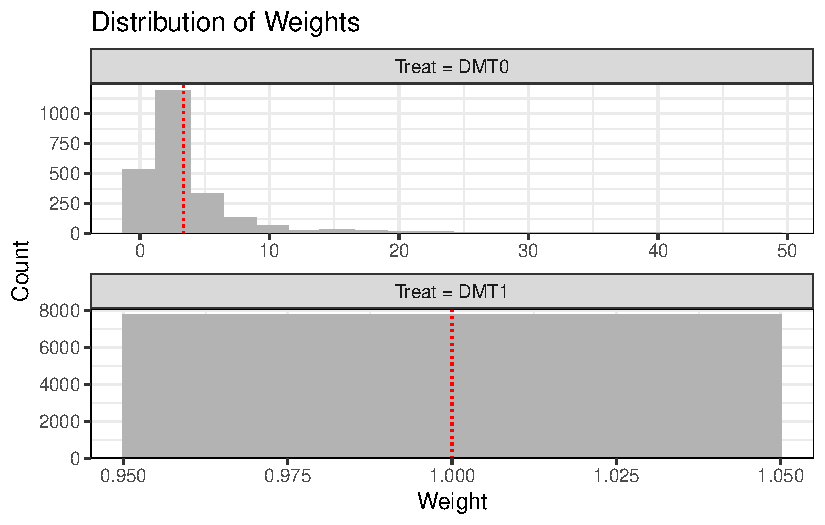
\includegraphics{chapter_06_files/figure-pdf/unnamed-chunk-32-1.pdf}

}

\end{figure}

\hypertarget{assess-balance-in-the-weighted-sample}{%
\subsection{Assess balance in the weighted
sample}\label{assess-balance-in-the-weighted-sample}}

\begin{Shaded}
\begin{Highlighting}[]
\FunctionTok{bal.tab}\NormalTok{(w.out, }\AttributeTok{stats =} \FunctionTok{c}\NormalTok{(}\StringTok{"m"}\NormalTok{, }\StringTok{"v"}\NormalTok{), }\AttributeTok{thresholds =} \FunctionTok{c}\NormalTok{(}\AttributeTok{m =}\NormalTok{ .}\DecValTok{05}\NormalTok{))}
\end{Highlighting}
\end{Shaded}

\begin{verbatim}
Balance Measures
                                         Type Diff.Adj     M.Threshold
prop.score                           Distance  -0.0045 Balanced, <0.05
age                                   Contin.   0.0054 Balanced, <0.05
female                                 Binary   0.0005 Balanced, <0.05
prevDMTefficacy_None                   Binary  -0.0003 Balanced, <0.05
prevDMTefficacy_Low_efficacy           Binary   0.0023 Balanced, <0.05
prevDMTefficacy_Medium_high_efficacy   Binary  -0.0020 Balanced, <0.05
prerelapse_num                        Contin.  -0.0034 Balanced, <0.05
                                     V.Ratio.Adj
prop.score                                0.9926
age                                       1.0102
female                                         .
prevDMTefficacy_None                           .
prevDMTefficacy_Low_efficacy                   .
prevDMTefficacy_Medium_high_efficacy           .
prerelapse_num                            1.0941

Balance tally for mean differences
                    count
Balanced, <0.05         7
Not Balanced, >0.05     0

Variable with the greatest mean difference
 Variable Diff.Adj     M.Threshold
      age   0.0054 Balanced, <0.05

Effective sample sizes
              DMT0 DMT1
Unadjusted 2300.   7700
Adjusted   1043.16 7700
\end{verbatim}

\hypertarget{estimate-the-att}{%
\subsection{Estimate the ATT}\label{estimate-the-att}}

One way to estimate the ATT is to use the survey package. The function
\texttt{svyglm()} generates model-robust (Horvitz-Thompson-type)
standard errors by default, and thus does not require additional
adjustments.

\begin{Shaded}
\begin{Highlighting}[]
\FunctionTok{library}\NormalTok{(survey)}

\NormalTok{weighted.data }\OtherTok{\textless{}{-}} \FunctionTok{svydesign}\NormalTok{(}\AttributeTok{ids =} \SpecialCharTok{\textasciitilde{}}\DecValTok{1}\NormalTok{, }\AttributeTok{data =}\NormalTok{ dat, }\AttributeTok{weights =} \SpecialCharTok{\textasciitilde{}}\NormalTok{w.out}\SpecialCharTok{$}\NormalTok{weights)}

\NormalTok{weighted.fit }\OtherTok{\textless{}{-}} \FunctionTok{svyglm}\NormalTok{(y }\SpecialCharTok{\textasciitilde{}}\NormalTok{ treatment }\SpecialCharTok{+} \FunctionTok{offset}\NormalTok{(}\FunctionTok{log}\NormalTok{(years)),}
                       \AttributeTok{family =} \FunctionTok{poisson}\NormalTok{(}\AttributeTok{link =} \StringTok{"log"}\NormalTok{),}
                       \AttributeTok{design =}\NormalTok{ weighted.data)}

\FunctionTok{exp}\NormalTok{(}\FunctionTok{coef}\NormalTok{(weighted.fit)[}\StringTok{"treatmentDMT1"}\NormalTok{])}
\end{Highlighting}
\end{Shaded}

\begin{verbatim}
treatmentDMT1 
    0.7083381 
\end{verbatim}

\begin{Shaded}
\begin{Highlighting}[]
\FunctionTok{exp}\NormalTok{(}\FunctionTok{confint}\NormalTok{(weighted.fit))[}\StringTok{"treatmentDMT1"}\NormalTok{,] }
\end{Highlighting}
\end{Shaded}

\begin{verbatim}
    2.5 %    97.5 % 
0.6245507 0.8033662 
\end{verbatim}

As indicated above, propensity score weighting yielded an ATT estimate
of 0.71 (95\% CI: 0.62; 0.8).

An alternative approach is to use \texttt{glm()} to estimate the
treatment effect and calculate robust standard errors.

\begin{Shaded}
\begin{Highlighting}[]
\CommentTok{\# Alternative way to estimate treatment effect}
\NormalTok{weighted.fit2 }\OtherTok{\textless{}{-}} \FunctionTok{glm}\NormalTok{(y }\SpecialCharTok{\textasciitilde{}}\NormalTok{ treatment }\SpecialCharTok{+} \FunctionTok{offset}\NormalTok{(}\FunctionTok{log}\NormalTok{(years)),}
              \AttributeTok{family =} \FunctionTok{poisson}\NormalTok{(}\AttributeTok{link =} \StringTok{"log"}\NormalTok{),}
              \AttributeTok{data =}\NormalTok{ dat,}
              \AttributeTok{weights =}\NormalTok{ w.out}\SpecialCharTok{$}\NormalTok{weights)}

\CommentTok{\# Extract the estimated ARR}
\FunctionTok{exp}\NormalTok{(}\FunctionTok{coef}\NormalTok{(weighted.fit2))[}\StringTok{"treatmentDMT1"}\NormalTok{]}
\end{Highlighting}
\end{Shaded}

\begin{verbatim}
treatmentDMT1 
    0.7083381 
\end{verbatim}

\begin{Shaded}
\begin{Highlighting}[]
\CommentTok{\# Calculate robust standard error and p{-}value of the log ARR}
\FunctionTok{coeftest}\NormalTok{(weighted.fit2, }\AttributeTok{vcov. =}\NormalTok{ vcovHC)[}\StringTok{"treatmentDMT1"}\NormalTok{,]}
\end{Highlighting}
\end{Shaded}

\begin{verbatim}
     Estimate    Std. Error       z value      Pr(>|z|) 
-3.448337e-01  6.442745e-02 -5.352280e+00  8.685284e-08 
\end{verbatim}

\begin{Shaded}
\begin{Highlighting}[]
\CommentTok{\# Derive 95\% confidence interval of the ARR}
\FunctionTok{exp}\NormalTok{(lmtest}\SpecialCharTok{::}\FunctionTok{coefci}\NormalTok{(weighted.fit2, }
       \AttributeTok{level =} \FloatTok{0.95}\NormalTok{, }\CommentTok{\# 95\% confidence interval}
       \AttributeTok{vcov. =}\NormalTok{ vcovHC)[}\StringTok{"treatmentDMT1"}\NormalTok{,])}
\end{Highlighting}
\end{Shaded}

\begin{verbatim}
    2.5 %    97.5 % 
0.6243094 0.8036767 
\end{verbatim}

Using this approach, the ATT estimate was 0.71 (95\% CI: 0.62; 0.8).

\hypertarget{regression-adjustment-for-the-propensity-score-for-the-ate}{%
\section{Regression adjustment for the propensity score for the
ATE}\label{regression-adjustment-for-the-propensity-score-for-the-ate}}

In this approach, a regression model is fitted to describe the observed
outcome as a function of the received treatment and the estimated
propensity score:

\begin{Shaded}
\begin{Highlighting}[]
\NormalTok{ps.reg.fit }\OtherTok{\textless{}{-}} \FunctionTok{glm}\NormalTok{(y }\SpecialCharTok{\textasciitilde{}}\NormalTok{ treatment }\SpecialCharTok{+}\NormalTok{ ps }\SpecialCharTok{+} \FunctionTok{offset}\NormalTok{(}\FunctionTok{log}\NormalTok{(years)),}
                  \AttributeTok{family =} \FunctionTok{poisson}\NormalTok{(}\AttributeTok{link =} \StringTok{"log"}\NormalTok{),}
                  \AttributeTok{data =}\NormalTok{ dat)}

\FunctionTok{summary}\NormalTok{(ps.reg.fit)}
\end{Highlighting}
\end{Shaded}

\begin{verbatim}

Call:
glm(formula = y ~ treatment + ps + offset(log(years)), family = poisson(link = "log"), 
    data = dat)

Deviance Residuals: 
    Min       1Q   Median       3Q      Max  
-2.0160  -0.7336  -0.4441  -0.1352   4.2634  

Coefficients:
              Estimate Std. Error z value Pr(>|z|)    
(Intercept)   -1.99585    0.10359 -19.266  < 2e-16 ***
treatmentDMT1 -0.25598    0.04431  -5.777 7.60e-09 ***
ps             1.07521    0.13878   7.748 9.36e-15 ***
---
Signif. codes:  0 '***' 0.001 '**' 0.01 '*' 0.05 '.' 0.1 ' ' 1

(Dispersion parameter for poisson family taken to be 1)

    Null deviance: 7514.7  on 9999  degrees of freedom
Residual deviance: 7443.0  on 9997  degrees of freedom
AIC: 12378

Number of Fisher Scoring iterations: 6
\end{verbatim}

\begin{Shaded}
\begin{Highlighting}[]
\CommentTok{\# ATE}
\FunctionTok{exp}\NormalTok{(}\FunctionTok{coef}\NormalTok{(ps.reg.fit))[}\StringTok{"treatmentDMT1"}\NormalTok{] }
\end{Highlighting}
\end{Shaded}

\begin{verbatim}
treatmentDMT1 
    0.7741606 
\end{verbatim}

\begin{verbatim}
Waiting for profiling to be done...
Waiting for profiling to be done...
\end{verbatim}

Bootstrapped confidence intervals can be obtained as follows:

\begin{Shaded}
\begin{Highlighting}[]
\CommentTok{\# Function to bootstrap for 95\% CIs}
\NormalTok{ps.reg.bootstrap }\OtherTok{\textless{}{-}} \ControlFlowTok{function}\NormalTok{(data, inds) \{}
\NormalTok{  d }\OtherTok{\textless{}{-}}\NormalTok{ data[inds,]}
  
\NormalTok{  fit }\OtherTok{\textless{}{-}} \FunctionTok{glm}\NormalTok{(y }\SpecialCharTok{\textasciitilde{}}\NormalTok{ treatment }\SpecialCharTok{+}\NormalTok{ ps }\SpecialCharTok{+} \FunctionTok{offset}\NormalTok{(}\FunctionTok{log}\NormalTok{(years)),}
              \AttributeTok{family =} \FunctionTok{poisson}\NormalTok{(}\AttributeTok{link =} \StringTok{"log"}\NormalTok{),}
              \AttributeTok{data =}\NormalTok{ d)}
  
  \FunctionTok{return}\NormalTok{(}\FunctionTok{exp}\NormalTok{(}\FunctionTok{coef}\NormalTok{(fit))[}\StringTok{"treatmentDMT1"}\NormalTok{])}
\NormalTok{\}}

\FunctionTok{set.seed}\NormalTok{(}\DecValTok{1854}\NormalTok{)}

\CommentTok{\# Generate 1000 bootstrap replicates}
\NormalTok{arr.boot }\OtherTok{\textless{}{-}} \FunctionTok{boot}\NormalTok{(dat, }\AttributeTok{statistic =}\NormalTok{ ps.reg.bootstrap, }\AttributeTok{R =} \DecValTok{1000}\NormalTok{) }

\CommentTok{\# Extract the median annualized relapse rate across 1000 bootstrap replicates}
\FunctionTok{median}\NormalTok{(arr.boot}\SpecialCharTok{$}\NormalTok{t) }
\end{Highlighting}
\end{Shaded}

\begin{verbatim}
[1] 0.7750426
\end{verbatim}

\begin{Shaded}
\begin{Highlighting}[]
\CommentTok{\# Take 2.5th and 97.5th percentiles to be 95\% CI}
\FunctionTok{quantile}\NormalTok{(arr.boot}\SpecialCharTok{$}\NormalTok{t[,}\DecValTok{1}\NormalTok{], }\FunctionTok{c}\NormalTok{(}\FloatTok{0.025}\NormalTok{, }\FloatTok{0.975}\NormalTok{)) }
\end{Highlighting}
\end{Shaded}

\begin{verbatim}
     2.5%     97.5% 
0.7010540 0.8545169 
\end{verbatim}

\hypertarget{overview}{%
\section{Overview}\label{overview}}

\begin{longtable}[]{@{}
  >{\raggedright\arraybackslash}p{(\columnwidth - 8\tabcolsep) * \real{0.5196}}
  >{\raggedright\arraybackslash}p{(\columnwidth - 8\tabcolsep) * \real{0.0882}}
  >{\raggedleft\arraybackslash}p{(\columnwidth - 8\tabcolsep) * \real{0.0980}}
  >{\raggedleft\arraybackslash}p{(\columnwidth - 8\tabcolsep) * \real{0.1471}}
  >{\raggedleft\arraybackslash}p{(\columnwidth - 8\tabcolsep) * \real{0.1471}}@{}}
\toprule\noalign{}
\begin{minipage}[b]{\linewidth}\raggedright
Method
\end{minipage} & \begin{minipage}[b]{\linewidth}\raggedright
Estimand
\end{minipage} & \begin{minipage}[b]{\linewidth}\raggedleft
Estimate
\end{minipage} & \begin{minipage}[b]{\linewidth}\raggedleft
95\% CI (lower)
\end{minipage} & \begin{minipage}[b]{\linewidth}\raggedleft
95\% CI (upper)
\end{minipage} \\
\midrule\noalign{}
\endhead
\bottomrule\noalign{}
\endlastfoot
Optimal full matching & ATT & 0.8039901 & 0.6040414 & 1.0039388 \\
Propensity score stratification & ATT & 0.7482462 & NA & NA \\
Propensity score stratification (with bootstrapping) & ATT & 0.7558609 &
0.6835885 & 0.8362947 \\
Propensity score weighting & ATT & 0.7083381 & 0.6245507 & 0.8033662 \\
Propensity score weighting (robust SE) & ATT & 0.7083381 & 0.6243094 &
0.8036767 \\
PS regression adjustment & ATE & 0.7741606 & 0.7101080 & 0.8448218 \\
PS regression adjustment (bootstrapping) & ATE & 0.7750426 & 0.7010540 &
0.8545169 \\
\end{longtable}

\hypertarget{version-info-1}{%
\section*{Version info}\label{version-info-1}}
\addcontentsline{toc}{section}{Version info}

\markright{Version info}

This chapter was rendered using the following version of R and its
packages:

\begin{verbatim}
R version 4.2.3 (2023-03-15 ucrt)
Platform: x86_64-w64-mingw32/x64 (64-bit)
Running under: Windows 10 x64 (build 19045)

Matrix products: default

locale:
[1] LC_COLLATE=Dutch_Netherlands.utf8  LC_CTYPE=Dutch_Netherlands.utf8   
[3] LC_MONETARY=Dutch_Netherlands.utf8 LC_NUMERIC=C                      
[5] LC_TIME=Dutch_Netherlands.utf8    

attached base packages:
[1] grid      stats     graphics  grDevices utils     datasets  methods  
[8] base     

other attached packages:
 [1] WeightIt_0.14.2        boot_1.3-28.1          MatchIt_4.5.4         
 [4] sandwich_3.0-2         truncnorm_1.0-9        tableone_0.13.2       
 [7] survey_4.2-1           survival_3.5-5         Matrix_1.5-4.1        
[10] MASS_7.3-60            marginaleffects_0.13.0 lmtest_0.9-40         
[13] zoo_1.8-12             knitr_1.43             ggplot2_3.4.2         
[16] data.table_1.14.8      cobalt_4.5.1           dplyr_1.1.2           

loaded via a namespace (and not attached):
 [1] tidyselect_1.2.0 xfun_0.39        mitools_2.4      splines_4.2.3   
 [5] haven_2.5.2      lattice_0.21-8   labelled_2.11.0  colorspace_2.1-0
 [9] vctrs_0.6.3      generics_0.1.3   htmltools_0.5.5  yaml_2.3.7      
[13] utf8_1.2.3       rlang_1.1.1      e1071_1.7-13     pillar_1.9.0    
[17] glue_1.6.2       withr_2.5.0      DBI_1.1.3        lifecycle_1.0.3 
[21] munsell_0.5.0    gtable_0.3.3     codetools_0.2-19 evaluate_0.21   
[25] labeling_0.4.2   forcats_1.0.0    fastmap_1.1.1    class_7.3-22    
[29] fansi_1.0.4      optmatch_0.10.6  Rcpp_1.0.10      checkmate_2.2.0 
[33] backports_1.4.1  scales_1.2.1     jsonlite_1.8.5   farver_2.1.1    
[37] chk_0.9.0        hms_1.1.3        digest_0.6.31    insight_0.19.2  
[41] cli_3.6.1        tools_4.2.3      magrittr_2.0.3   proxy_0.4-27    
[45] tibble_3.2.1     crayon_1.5.2     pkgconfig_2.0.3  rlemon_0.2.1    
[49] rmarkdown_2.22   rstudioapi_0.14  R6_2.5.1         compiler_4.2.3  
\end{verbatim}

\hypertarget{references}{%
\section*{References}\label{references}}
\addcontentsline{toc}{section}{References}

\markright{References}

\bookmarksetup{startatroot}

\hypertarget{effect-modification-analysis-within-the-propensity-score-framework}{%
\chapter{Effect Modification Analysis within the Propensity score
Framework}\label{effect-modification-analysis-within-the-propensity-score-framework}}

Mohammad Ehsanul Karim (University of British Columbia)

\hfill\break

Observational comparative effectiveness studies often adopt propensity
score analysis to adjust for confounding. Although this approach is
relatively straightforward to implement, careful thought is needed when
treatment effect heterogeneity is present. This chapter illustrates the
estimation of subgroup-specific treatment effects using (traditional)
covariate adjustment methods, propensity score matching, propensity
score weighting, propensity score stratification, and covariate
adjustment using propensity scores.

\hypertarget{simulation}{%
\section{Simulation}\label{simulation}}

First, we need to install the R package \texttt{simcausal}, which can be
obtained from GitHub:

\begin{Shaded}
\begin{Highlighting}[]
\NormalTok{devtools}\SpecialCharTok{::}\FunctionTok{install\_github}\NormalTok{(}\StringTok{\textquotesingle{}osofr/simcausal\textquotesingle{}}\NormalTok{, }\AttributeTok{build\_vignettes =} \ConstantTok{FALSE}\NormalTok{)}
\end{Highlighting}
\end{Shaded}

We will use the following data-generation model:

\begin{Shaded}
\begin{Highlighting}[]
\FunctionTok{require}\NormalTok{(simcausal)}
\NormalTok{D }\OtherTok{\textless{}{-}} \FunctionTok{DAG.empty}\NormalTok{()}
\NormalTok{D }\OtherTok{\textless{}{-}}\NormalTok{ D }\SpecialCharTok{+} 
  \FunctionTok{node}\NormalTok{(}\StringTok{"age"}\NormalTok{, }\AttributeTok{distr =} \StringTok{"rnorm"}\NormalTok{, }
       \AttributeTok{mean =} \DecValTok{2}\NormalTok{, }\AttributeTok{sd =} \DecValTok{4}\NormalTok{) }\SpecialCharTok{+} 
  \FunctionTok{node}\NormalTok{(}\StringTok{"gender"}\NormalTok{, }\AttributeTok{distr =} \StringTok{"rbern"}\NormalTok{, }
       \AttributeTok{prob =} \FunctionTok{plogis}\NormalTok{(}\DecValTok{4}\NormalTok{)) }\SpecialCharTok{+}
  \FunctionTok{node}\NormalTok{(}\StringTok{"education"}\NormalTok{, }\AttributeTok{distr =} \StringTok{"rbern"}\NormalTok{, }
       \AttributeTok{prob =} \FunctionTok{plogis}\NormalTok{(}\DecValTok{3} \SpecialCharTok{+} \DecValTok{5} \SpecialCharTok{*}\NormalTok{ age)) }\SpecialCharTok{+}
  \FunctionTok{node}\NormalTok{(}\StringTok{"diet"}\NormalTok{, }\AttributeTok{distr =} \StringTok{"rbern"}\NormalTok{, }
       \AttributeTok{prob =} \FunctionTok{plogis}\NormalTok{(}\DecValTok{1} \SpecialCharTok{{-}} \DecValTok{3} \SpecialCharTok{*}\NormalTok{ education)) }\SpecialCharTok{+}
  \FunctionTok{node}\NormalTok{(}\StringTok{"income"}\NormalTok{, }\AttributeTok{distr =} \StringTok{"rbern"}\NormalTok{, }
       \AttributeTok{prob =} \FunctionTok{plogis}\NormalTok{(}\DecValTok{2} \SpecialCharTok{{-}} \DecValTok{5} \SpecialCharTok{*}\NormalTok{ education }\SpecialCharTok{{-}} \DecValTok{4} \SpecialCharTok{*}\NormalTok{ age)) }\SpecialCharTok{+}
  \FunctionTok{node}\NormalTok{(}\StringTok{"smoking"}\NormalTok{, }\AttributeTok{distr =} \StringTok{"rbern"}\NormalTok{, }
       \AttributeTok{prob =} \FunctionTok{plogis}\NormalTok{(}\DecValTok{1} \SpecialCharTok{+} \FloatTok{1.2} \SpecialCharTok{*}\NormalTok{ gender }\SpecialCharTok{+} \DecValTok{2} \SpecialCharTok{*}\NormalTok{ age)) }\SpecialCharTok{+}
  \FunctionTok{node}\NormalTok{(}\StringTok{"hypertension"}\NormalTok{, }\AttributeTok{distr =} \StringTok{"rbern"}\NormalTok{, }
       \AttributeTok{prob =} \FunctionTok{plogis}\NormalTok{(}\DecValTok{1} \SpecialCharTok{+} \FunctionTok{log}\NormalTok{(}\DecValTok{3}\NormalTok{) }\SpecialCharTok{*}\NormalTok{ diet }\SpecialCharTok{+} 
                       \FunctionTok{log}\NormalTok{(}\FloatTok{1.3}\NormalTok{) }\SpecialCharTok{*}\NormalTok{ age }\SpecialCharTok{+} 
                       \FunctionTok{log}\NormalTok{(}\FloatTok{3.5}\NormalTok{) }\SpecialCharTok{*}\NormalTok{ smoking }\SpecialCharTok{+} 
                       \FunctionTok{log}\NormalTok{(}\FloatTok{0.5}\NormalTok{) }\SpecialCharTok{*}\NormalTok{ gender))}
\NormalTok{Dset }\OtherTok{\textless{}{-}} \FunctionTok{set.DAG}\NormalTok{(D)}
\end{Highlighting}
\end{Shaded}

Below is the diagram, with pink lines representing open backdoor path.

\begin{verbatim}
using the following vertex attributes: 
\end{verbatim}

\begin{verbatim}
NAdarkbluenone100.50
\end{verbatim}

\begin{verbatim}
using the following edge attributes: 
\end{verbatim}

\begin{verbatim}
black0.210.60.5
\end{verbatim}

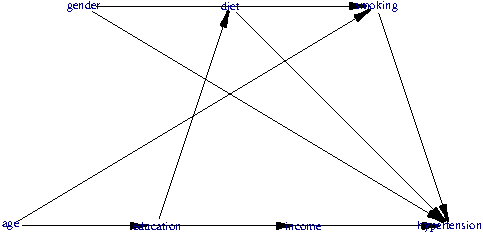
\includegraphics{chapter_07_files/figure-pdf/unnamed-chunk-4-1.pdf}

We can now generate an example dataset:

\begin{Shaded}
\begin{Highlighting}[]
\NormalTok{Obs.Data }\OtherTok{\textless{}{-}} \FunctionTok{sim}\NormalTok{(}\AttributeTok{DAG =}\NormalTok{ Dset, }\AttributeTok{n =} \DecValTok{50000}\NormalTok{, }\AttributeTok{rndseed =} \DecValTok{123}\NormalTok{)}
\NormalTok{Obs.Data}\SpecialCharTok{$}\NormalTok{smoking }\OtherTok{\textless{}{-}} \FunctionTok{as.character}\NormalTok{(Obs.Data}\SpecialCharTok{$}\NormalTok{smoking)}
\NormalTok{Obs.Data}\SpecialCharTok{$}\NormalTok{income }\OtherTok{\textless{}{-}} \FunctionTok{as.factor}\NormalTok{(Obs.Data}\SpecialCharTok{$}\NormalTok{income)}
\NormalTok{Obs.Data}\SpecialCharTok{$}\NormalTok{income }\OtherTok{\textless{}{-}} \FunctionTok{relevel}\NormalTok{(Obs.Data}\SpecialCharTok{$}\NormalTok{income, }\AttributeTok{ref =} \StringTok{"1"}\NormalTok{)}
\end{Highlighting}
\end{Shaded}

Sample data from the hypothetical example of association between
hypertension and smoking, where other variables such as income, age
{[}centered{]}, gender, education and diet also plays a role in the data
generation process.

\begin{table}[!h]
\centering
\begin{tabular}{lrrrrllr}
\toprule
  & age & gender & education & diet & income & smoking & hypertension\\
\midrule
34901 & 12.29 & 1 & 1 & 1 & 0 & 1 & 1\\
149 & 10.40 & 1 & 1 & 0 & 0 & 1 & 1\\
10060 & 2.99 & 1 & 1 & 0 & 0 & 1 & 0\\
22220 & -4.31 & 0 & 0 & 0 & 1 & 0 & 1\\
9979 & -6.44 & 0 & 0 & 0 & 1 & 0 & 1\\
\bottomrule
\end{tabular}
\end{table}

\hypertarget{covariate-adjustment}{%
\section{Covariate adjustment}\label{covariate-adjustment}}

\hypertarget{interaction-approach}{%
\subsection{Interaction approach}\label{interaction-approach}}

Below, we estimate a logistic regression model to assess whether the
effect of smoking (the exposure) on hypertension is modified by income
levels. This model considers the following variables:

\begin{itemize}
\tightlist
\item
  Outcome: \texttt{hypertension}
\item
  Exposure variables: \texttt{smoking} and \texttt{income}
\item
  Confounders: \texttt{age} and \texttt{gender}
\end{itemize}

\begin{Shaded}
\begin{Highlighting}[]
\FunctionTok{require}\NormalTok{(jtools)}

\NormalTok{fit.w.em }\OtherTok{\textless{}{-}} \FunctionTok{glm}\NormalTok{(hypertension }\SpecialCharTok{\textasciitilde{}}\NormalTok{ smoking }\SpecialCharTok{*}\NormalTok{ income }\SpecialCharTok{+}\NormalTok{ age }\SpecialCharTok{+}\NormalTok{ gender, }
            \AttributeTok{family =} \FunctionTok{binomial}\NormalTok{(}\AttributeTok{link =} \StringTok{"logit"}\NormalTok{), }\AttributeTok{data =}\NormalTok{ Obs.Data)}

\NormalTok{results.model }\OtherTok{\textless{}{-}} \FunctionTok{summ}\NormalTok{(fit.w.em, }\AttributeTok{exp =} \ConstantTok{TRUE}\NormalTok{)}
\end{Highlighting}
\end{Shaded}

\begin{table}[!h]
\centering
\begin{tabular}{lrrrrr}
\toprule
  & exp(Est.) & 2.5\% & 97.5\% & z val. & p\\
\midrule
(Intercept) & 5.46 & 4.37 & 6.82 & 14.97 & 0.00\\
smoking1 & 2.93 & 2.60 & 3.30 & 17.69 & 0.00\\
income0 & 0.48 & 0.41 & 0.57 & -8.28 & 0.00\\
age & 1.29 & 1.27 & 1.31 & 36.77 & 0.00\\
gender & 0.54 & 0.43 & 0.67 & -5.55 & 0.00\\
\addlinespace
smoking1:income0 & 1.27 & 1.04 & 1.56 & 2.33 & 0.02\\
\bottomrule
\end{tabular}
\end{table}

Results indicate that the interaction between smoking status and income
level is statistically significant (p = 0.02).

If we expand previous model to adjust for an additional confounder
\texttt{education}, we have:

\begin{Shaded}
\begin{Highlighting}[]
\NormalTok{fit.w.int }\OtherTok{\textless{}{-}} \FunctionTok{glm}\NormalTok{(hypertension }\SpecialCharTok{\textasciitilde{}}\NormalTok{ smoking }\SpecialCharTok{*}\NormalTok{ income }\SpecialCharTok{+}\NormalTok{ age }\SpecialCharTok{+}\NormalTok{ gender }\SpecialCharTok{+}\NormalTok{ education, }
                 \AttributeTok{family =} \FunctionTok{binomial}\NormalTok{(}\AttributeTok{link =} \StringTok{"logit"}\NormalTok{), }
                 \AttributeTok{data =}\NormalTok{ Obs.Data)}

\NormalTok{results.int.model }\OtherTok{\textless{}{-}} \FunctionTok{summ}\NormalTok{(fit.w.int, }\AttributeTok{exp =} \ConstantTok{TRUE}\NormalTok{)}
\end{Highlighting}
\end{Shaded}

\begin{table}[!h]
\centering
\begin{tabular}{lrrrrr}
\toprule
  & exp(Est.) & 2.5\% & 97.5\% & z val. & p\\
\midrule
(Intercept) & 5.69 & 4.56 & 7.11 & 15.31 & 0.00\\
smoking1 & 3.35 & 2.95 & 3.79 & 18.85 & 0.00\\
income0 & 1.09 & 0.85 & 1.40 & 0.68 & 0.49\\
age & 1.30 & 1.28 & 1.32 & 37.32 & 0.00\\
gender & 0.54 & 0.43 & 0.67 & -5.58 & 0.00\\
\addlinespace
education & 0.42 & 0.35 & 0.51 & -8.87 & 0.00\\
smoking1:income0 & 1.10 & 0.90 & 1.35 & 0.93 & 0.35\\
\bottomrule
\end{tabular}
\end{table}

The interaction term between income and smoking is no longer
statistically significant (p = 0.35).

We can generate a summary report from aforementioned effect modification
analysis.

\begin{Shaded}
\begin{Highlighting}[]
\FunctionTok{require}\NormalTok{(interactionR)}

\NormalTok{em.object }\OtherTok{\textless{}{-}} \FunctionTok{interactionR}\NormalTok{(fit.w.em, }
                          \AttributeTok{exposure\_names =} \FunctionTok{c}\NormalTok{(}\StringTok{"income0"}\NormalTok{, }\StringTok{"smoking1"}\NormalTok{), }
                          \AttributeTok{ci.type =} \StringTok{"mover"}\NormalTok{, }\AttributeTok{ci.level =} \FloatTok{0.95}\NormalTok{, }
                          \AttributeTok{em =} \ConstantTok{TRUE}\NormalTok{, }\AttributeTok{recode =} \ConstantTok{FALSE}\NormalTok{)}
\end{Highlighting}
\end{Shaded}

The table below depicts the adjusted odds ratios for income levels
(\texttt{high\ =\ 0}, and \texttt{low\ =\ 1}). The variables
\texttt{CI.ll} and \texttt{CI.ul} depict the lower and upper limits of
the 95 percent confidence intervals, \texttt{OR11} =
\(OR_{A = 1, M = 1}\) , \texttt{OR10} = \(OR_{A = 1}\), \texttt{OR01} =
\(OR_{M = 1}\) and \texttt{OR00} captures the reference.

\hypertarget{tbl-effint-fit.w.em}{}
\begin{table}[!h]
\caption{\label{tbl-effint-fit.w.em}Summary report from an interaction analysis when investigating
association between two exposure variables (smoking and income) and
hypertension. }\tabularnewline

\centering
\begin{tabular}{lrrr}
\toprule
Measures & Estimates & CI.ll & CI.ul\\
\midrule
OR00 & 1.00 & NA & NA\\
OR01 & 2.93 & 2.60 & 3.30\\
OR10 & 0.48 & 0.41 & 0.57\\
OR11 & 1.80 & 1.63 & 1.98\\
OR(smoking1 on outcome [income0==0] & 2.93 & 2.60 & 3.30\\
\addlinespace
OR(smoking1 on outcome [income0==1] & 3.72 & 3.14 & 4.41\\
Multiplicative scale & 1.27 & 1.04 & 1.56\\
RERI & -0.61 & -0.98 & -0.29\\
\bottomrule
\end{tabular}
\end{table}

Similarly, for the analysis adjusting for an additional confounder
\texttt{education}, we have:

\hypertarget{tbl-effint-fit.w.int}{}
\begin{table}[!h]
\caption{\label{tbl-effint-fit.w.int}Summary report from an interaction analysis when investigating
association between two exposure variables (smoking and income) and
hypertension. }\tabularnewline

\centering
\begin{tabular}{lrrr}
\toprule
Measures & Estimates & CI.ll & CI.ul\\
\midrule
OR00 & 1.00 & NA & NA\\
OR01 & 1.09 & 0.85 & 1.40\\
OR10 & 3.35 & 2.95 & 3.79\\
OR11 & 4.02 & 3.29 & 4.92\\
OR(income0 on outcome [smoking1==0] & 1.09 & 0.85 & 1.40\\
\addlinespace
OR(income0 on outcome [smoking1==1] & 1.20 & 1.00 & 1.45\\
OR(smoking1 on outcome [income0==0] & 3.35 & 2.95 & 3.79\\
OR(smoking1 on outcome [income0==1] & 3.69 & 3.11 & 4.37\\
Multiplicative scale & 1.10 & 0.90 & 1.35\\
RERI & 0.59 & 0.03 & 1.27\\
\addlinespace
AP & 0.15 & 0.00 & 0.26\\
SI & 1.24 & 1.01 & 1.53\\
\bottomrule
\end{tabular}
\end{table}

\begin{Shaded}
\begin{Highlighting}[]
\CommentTok{\# test run with additive model}
\NormalTok{Obs.Data}\SpecialCharTok{$}\NormalTok{smoking }\OtherTok{\textless{}{-}} \FunctionTok{as.numeric}\NormalTok{(}\FunctionTok{as.character}\NormalTok{(Obs.Data}\SpecialCharTok{$}\NormalTok{smoking))}
\NormalTok{Obs.Data}\SpecialCharTok{$}\NormalTok{income }\OtherTok{\textless{}{-}} \FunctionTok{as.numeric}\NormalTok{(}\FunctionTok{as.character}\NormalTok{(Obs.Data}\SpecialCharTok{$}\NormalTok{income))}
\NormalTok{fit.w.int.add }\OtherTok{\textless{}{-}} \FunctionTok{glm}\NormalTok{(hypertension }\SpecialCharTok{\textasciitilde{}}\NormalTok{ smoking }\SpecialCharTok{*}\NormalTok{ income }\SpecialCharTok{+}\NormalTok{ age }\SpecialCharTok{+}\NormalTok{ gender }\SpecialCharTok{+}\NormalTok{ education, }
                     \AttributeTok{family =} \FunctionTok{gaussian}\NormalTok{(}\AttributeTok{link =} \StringTok{"identity"}\NormalTok{), }\AttributeTok{data =}\NormalTok{ Obs.Data)}
\FunctionTok{sim\_slopes}\NormalTok{(fit.w.int.add, }\AttributeTok{pred =}\NormalTok{ smoking, }\AttributeTok{modx =}\NormalTok{ income,}
           \AttributeTok{exp =} \ConstantTok{TRUE}\NormalTok{, }\AttributeTok{robust =} \ConstantTok{TRUE}\NormalTok{,}
           \AttributeTok{confint =} \ConstantTok{TRUE}\NormalTok{, }\AttributeTok{data =}\NormalTok{ Obs.Dat)}
\end{Highlighting}
\end{Shaded}

\begin{verbatim}
JOHNSON-NEYMAN INTERVAL 

When income is INSIDE the interval [-3.27, 16.87], the slope of smoking is
p < .05.

Note: The range of observed values of income is [0.00, 1.00]

SIMPLE SLOPES ANALYSIS 

Slope of smoking when income = 0.00 (0): 

  Est.   S.E.   2.5%   97.5%   t val.      p
------ ------ ------ ------- -------- ------
  0.25   0.02   1.24    1.34    12.76   0.00

Slope of smoking when income = 1.00 (1): 

  Est.   S.E.   2.5%   97.5%   t val.      p
------ ------ ------ ------- -------- ------
  0.28   0.01   1.30    1.34    34.53   0.00
\end{verbatim}

\hypertarget{stratification}{%
\subsection{Stratification}\label{stratification}}

This approach involves estimating a regression model in different strata
of the discrete effect modifier \texttt{income}:

\begin{Shaded}
\begin{Highlighting}[]
\CommentTok{\# Estimate the prognostic effect of smoking in low income individuals}
\NormalTok{fit.income1 }\OtherTok{\textless{}{-}} \FunctionTok{glm}\NormalTok{(hypertension }\SpecialCharTok{\textasciitilde{}}\NormalTok{ smoking }\SpecialCharTok{+}\NormalTok{ age }\SpecialCharTok{+}\NormalTok{ gender, }
            \AttributeTok{family =} \FunctionTok{binomial}\NormalTok{(}\AttributeTok{link =} \StringTok{"logit"}\NormalTok{), }
            \AttributeTok{data =} \FunctionTok{subset}\NormalTok{(Obs.Data, income }\SpecialCharTok{==} \DecValTok{1}\NormalTok{))}

\CommentTok{\# Estimate the prognostic effect of smoking in high income individuals}
\NormalTok{fit.income0 }\OtherTok{\textless{}{-}} \FunctionTok{glm}\NormalTok{(hypertension }\SpecialCharTok{\textasciitilde{}}\NormalTok{ smoking }\SpecialCharTok{+}\NormalTok{ age }\SpecialCharTok{+}\NormalTok{ gender, }
            \AttributeTok{family =} \FunctionTok{binomial}\NormalTok{(}\AttributeTok{link =} \StringTok{"logit"}\NormalTok{), }
            \AttributeTok{data =} \FunctionTok{subset}\NormalTok{(Obs.Data, income }\SpecialCharTok{==} \DecValTok{0}\NormalTok{))}
\end{Highlighting}
\end{Shaded}

The table below summarizes the adjusted odds ratios for smoking across
the different income levels (\texttt{low\ =\ 1}, and
\texttt{high\ =\ 0}) as obtained using the stratified approach.

\begin{table}[!h]
\centering
\begin{tabular}{rrrrrr}
\toprule
Value of income & Estimate & 2.5 \% & 97.5 \% & z value & p value\\
\midrule
1 & 3.07 & 2.71 & 3.47 & 17.65 & 0\\
0 & 3.59 & 3.02 & 4.26 & 14.57 & 0\\
\bottomrule
\end{tabular}
\end{table}

Note that we can obtain the same results by estimating a regression
model with an interaction term between the modifier and all covariates:

\begin{Shaded}
\begin{Highlighting}[]
\NormalTok{fit.all.int }\OtherTok{\textless{}{-}} \FunctionTok{glm}\NormalTok{(hypertension }\SpecialCharTok{\textasciitilde{}}\NormalTok{ income }\SpecialCharTok{*}\NormalTok{ (smoking }\SpecialCharTok{+}\NormalTok{ age }\SpecialCharTok{+}\NormalTok{ gender), }
                   \AttributeTok{family =} \FunctionTok{binomial}\NormalTok{(}\AttributeTok{link =} \StringTok{"logit"}\NormalTok{), }\AttributeTok{data =}\NormalTok{ Obs.Data)}

\CommentTok{\# Odds ratio for smoking in individuals with low income }
\FunctionTok{exp}\NormalTok{(}\FunctionTok{coef}\NormalTok{(fit.all.int)[}\StringTok{"smoking"}\NormalTok{])}
\end{Highlighting}
\end{Shaded}

\begin{verbatim}
smoking 
3.59026 
\end{verbatim}

\begin{Shaded}
\begin{Highlighting}[]
\CommentTok{\# Odds ratio for smoking in individuals with high income}
\FunctionTok{exp}\NormalTok{(}\FunctionTok{coef}\NormalTok{(fit.all.int)[}\StringTok{"smoking"}\NormalTok{] }\SpecialCharTok{+} \FunctionTok{coef}\NormalTok{(fit.all.int)[}\StringTok{"income:smoking"}\NormalTok{])}
\end{Highlighting}
\end{Shaded}

\begin{verbatim}
 smoking 
3.066878 
\end{verbatim}

\hypertarget{propensity-score-matching-1}{%
\section{Propensity score matching}\label{propensity-score-matching-1}}

\hypertarget{stratification-with-exact-matching-within-subgroups}{%
\subsection{Stratification with exact matching within
subgroups}\label{stratification-with-exact-matching-within-subgroups}}

We simulate another example dataset using aforementioned DAG, but
restrict the sample size to 5000 individuals to reduce computational
burden.

\begin{Shaded}
\begin{Highlighting}[]
\FunctionTok{set.seed}\NormalTok{(}\DecValTok{123}\NormalTok{)}
\NormalTok{Obs.Data }\OtherTok{\textless{}{-}} \FunctionTok{sim}\NormalTok{(}\AttributeTok{DAG =}\NormalTok{ Dset, }\AttributeTok{n =} \DecValTok{5000}\NormalTok{, }\AttributeTok{rndseed =} \DecValTok{123}\NormalTok{)}
\end{Highlighting}
\end{Shaded}

We first estimate the propensity of smoking in the high-income group
(\texttt{income\ ==\ 0}):

\begin{Shaded}
\begin{Highlighting}[]
\FunctionTok{require}\NormalTok{(MatchIt)}

\NormalTok{match.income}\FloatTok{.0} \OtherTok{\textless{}{-}} \FunctionTok{matchit}\NormalTok{(smoking }\SpecialCharTok{\textasciitilde{}}\NormalTok{ age }\SpecialCharTok{+}\NormalTok{ gender, }
                          \AttributeTok{data =} \FunctionTok{subset}\NormalTok{(Obs.Data, income }\SpecialCharTok{==} \DecValTok{0}\NormalTok{),}
                          \AttributeTok{method =} \StringTok{"full"}\NormalTok{, }\AttributeTok{distance =} \StringTok{"glm"}\NormalTok{, }\AttributeTok{link =} \StringTok{"logit"}\NormalTok{)}
\NormalTok{data.income}\FloatTok{.0} \OtherTok{\textless{}{-}} \FunctionTok{match.data}\NormalTok{(match.income}\FloatTok{.0}\NormalTok{)}
\end{Highlighting}
\end{Shaded}

Below, we draw a sample from the high-income group based on the
hypothetical example of an association between hypertension and smoking.
Here age {[}centered{]}, gender, education, and diet are covariates.

\begin{verbatim}
            age gender education diet income smoking hypertension  distance
657   6.0810120      0         1    1      0       1            1 0.9999874
4932  1.6109860      1         1    0      0       1            0 0.9943155
252  -0.2475055      1         1    1      0       0            1 0.8525107
2693 -0.2511048      1         1    0      0       1            1 0.8516785
1646 -0.2836155      1         0    1      0       1            1 0.8439843
        weights subclass
657  1.00000000       36
4932 1.00000000       50
252  0.03296089       25
2693 1.00000000       25
1646 1.00000000        4
\end{verbatim}

Now, we do the same for the low-income group (\texttt{income\ ==\ 1}):

\begin{Shaded}
\begin{Highlighting}[]
\NormalTok{match.income}\FloatTok{.1} \OtherTok{\textless{}{-}} \FunctionTok{matchit}\NormalTok{(smoking }\SpecialCharTok{\textasciitilde{}}\NormalTok{ age }\SpecialCharTok{+}\NormalTok{ gender, }
                          \AttributeTok{data =} \FunctionTok{subset}\NormalTok{(Obs.Data, income }\SpecialCharTok{==} \DecValTok{1}\NormalTok{),}
                          \AttributeTok{method =} \StringTok{"full"}\NormalTok{, }\AttributeTok{distance =} \StringTok{"glm"}\NormalTok{, }\AttributeTok{link =} \StringTok{"logit"}\NormalTok{)}
\NormalTok{data.income}\FloatTok{.1} \OtherTok{\textless{}{-}} \FunctionTok{match.data}\NormalTok{(match.income}\FloatTok{.1}\NormalTok{)}
\end{Highlighting}
\end{Shaded}

We estimated the exposure effect from a weighted outcome model for the
matched data. While the \texttt{weights} are essential for estimating
the point estimate from the outcome model, the \texttt{subclass}
variable assists in calculating the robust variance of the exposure
effect estimate.

\begin{Shaded}
\begin{Highlighting}[]
\CommentTok{\# Treatment effect estimation}
\NormalTok{fit.income}\FloatTok{.0} \OtherTok{\textless{}{-}} \FunctionTok{glm}\NormalTok{(hypertension }\SpecialCharTok{\textasciitilde{}}\NormalTok{ smoking }\SpecialCharTok{+}\NormalTok{ age }\SpecialCharTok{+}\NormalTok{ gender, }
                   \AttributeTok{data =}\NormalTok{ data.income}\FloatTok{.0}\NormalTok{, }\AttributeTok{weights =}\NormalTok{ weights,}
                   \AttributeTok{family =} \FunctionTok{binomial}\NormalTok{(}\StringTok{"logit"}\NormalTok{))}
\NormalTok{fit.income}\FloatTok{.1} \OtherTok{\textless{}{-}} \FunctionTok{glm}\NormalTok{(hypertension }\SpecialCharTok{\textasciitilde{}}\NormalTok{ smoking }\SpecialCharTok{+}\NormalTok{ age }\SpecialCharTok{+}\NormalTok{ gender, }
                   \AttributeTok{data =}\NormalTok{ data.income}\FloatTok{.1}\NormalTok{, }\AttributeTok{weights =}\NormalTok{ weights,}
                   \AttributeTok{family =} \FunctionTok{binomial}\NormalTok{(}\StringTok{"logit"}\NormalTok{))}
\CommentTok{\# Robust variance calculation}
\NormalTok{fit.nexp.adj.res1 }\OtherTok{\textless{}{-}} \FunctionTok{summ}\NormalTok{(fit.income}\FloatTok{.1}\NormalTok{,  }
                          \AttributeTok{robust =} \ConstantTok{TRUE}\NormalTok{,}
                          \AttributeTok{cluster =} \StringTok{"subclass"}\NormalTok{,}
                          \AttributeTok{confint =} \ConstantTok{TRUE}\NormalTok{)}
\NormalTok{fit.nexp.adj.res0 }\OtherTok{\textless{}{-}} \FunctionTok{summ}\NormalTok{(fit.income}\FloatTok{.0}\NormalTok{, }
                          \AttributeTok{robust =} \ConstantTok{TRUE}\NormalTok{,}
                          \AttributeTok{cluster =} \StringTok{"subclass"}\NormalTok{,}
                          \AttributeTok{confint =} \ConstantTok{TRUE}\NormalTok{)}
\end{Highlighting}
\end{Shaded}

\hypertarget{tbl-stratified-approach}{}
\begin{table}[!h]
\caption{\label{tbl-stratified-approach}Subgroup-specific treatment effect estimates (expressed in log-OR) from
the hypothetical example using the stratified approach. }\tabularnewline

\centering
\begin{tabular}{rrrrrr}
\toprule
Value of income & Est. & 2.5\% & 97.5\% & z val. & p\\
\midrule
0 & 3.74 & -37.58 & 45.06 & 0.18 & 0.86\\
1 & 1.39 & 0.94 & 1.85 & 6.04 & 0.00\\
\bottomrule
\end{tabular}
\end{table}

\hypertarget{joint-approach-without-exact-matching-within-subgroups}{%
\subsection{Joint approach without exact matching within
subgroups}\label{joint-approach-without-exact-matching-within-subgroups}}

Here, entire cohort data is used to estimate the propensity scores, and
the effect modifier \texttt{income} is considered as a covariate in the
propensity score model:

\begin{Shaded}
\begin{Highlighting}[]
\NormalTok{ps.formula }\OtherTok{\textless{}{-}} \FunctionTok{as.formula}\NormalTok{(}\StringTok{"smoking \textasciitilde{} age + gender + income"}\NormalTok{)}
\NormalTok{match.obj.j }\OtherTok{\textless{}{-}} \FunctionTok{matchit}\NormalTok{(ps.formula, }\AttributeTok{data =}\NormalTok{ Obs.Data,}
                      \AttributeTok{method =} \StringTok{"full"}\NormalTok{, }
                      \AttributeTok{distance =} \StringTok{"glm"}\NormalTok{,}
                      \AttributeTok{link =} \StringTok{"logit"}\NormalTok{)}
\NormalTok{match.data.j }\OtherTok{\textless{}{-}} \FunctionTok{match.data}\NormalTok{(match.obj.j)}
\end{Highlighting}
\end{Shaded}

\begin{Shaded}
\begin{Highlighting}[]
\NormalTok{fit.joint.no.exact }\OtherTok{\textless{}{-}} \FunctionTok{glm}\NormalTok{(hypertension }\SpecialCharTok{\textasciitilde{}}\NormalTok{ smoking}\SpecialCharTok{*}\NormalTok{income }\SpecialCharTok{+}\NormalTok{ age }\SpecialCharTok{+}\NormalTok{ gender, }
                          \AttributeTok{data =}\NormalTok{ match.data.j, }
                          \AttributeTok{weights =}\NormalTok{ weights,}
                          \AttributeTok{family =} \FunctionTok{binomial}\NormalTok{(}\StringTok{"logit"}\NormalTok{))}
\FunctionTok{require}\NormalTok{(interactions)}
\NormalTok{nem.nexp.adj.res }\OtherTok{\textless{}{-}} \FunctionTok{sim\_slopes}\NormalTok{(fit.joint.no.exact, }
                               \AttributeTok{pred =}\NormalTok{ smoking, }
                               \AttributeTok{modx =}\NormalTok{ income,}
                               \AttributeTok{robust =} \StringTok{"HC1"}\NormalTok{, }
                               \AttributeTok{cluster =} \StringTok{"subclass"}\NormalTok{,}
                               \AttributeTok{johnson\_neyman =} \ConstantTok{TRUE}\NormalTok{, }
                               \AttributeTok{confint =} \ConstantTok{TRUE}\NormalTok{,}
                               \AttributeTok{data =}\NormalTok{ match.data.j)}
\end{Highlighting}
\end{Shaded}

\hypertarget{tbl-joint-approach}{}
\begin{table}[!h]
\caption{\label{tbl-joint-approach}Subgroup-specific treatment effect estimates (expressed in log-OR) from
the hypothetical example using the joint approach. }\tabularnewline

\centering
\begin{tabular}{r|r|r|r|r|r|r}
\hline
Value of income & Est. & S.E. & 2.5\% & 97.5\% & z val. & p\\
\hline
0 & 3.85 & 1.00 & 1.89 & 5.82 & 3.84 & 0\\
\hline
1 & 1.40 & 0.28 & 0.85 & 1.95 & 4.99 & 0\\
\hline
\end{tabular}
\end{table}

\hypertarget{joint-approach-with-exact-matching-within-subgroups}{%
\subsection{Joint approach with exact matching within
subgroups}\label{joint-approach-with-exact-matching-within-subgroups}}

We specify the moderator variable's name in the \texttt{exact} argument
of the \texttt{matchit} function.

\begin{Shaded}
\begin{Highlighting}[]
\NormalTok{ps.formula.no.mod }\OtherTok{\textless{}{-}} \FunctionTok{as.formula}\NormalTok{(}\StringTok{"smoking \textasciitilde{} age + gender"}\NormalTok{)}
\NormalTok{match.obj.js }\OtherTok{\textless{}{-}} \FunctionTok{matchit}\NormalTok{(ps.formula.no.mod, }\AttributeTok{data =}\NormalTok{ Obs.Data,}
                        \AttributeTok{method =} \StringTok{"full"}\NormalTok{, }\AttributeTok{distance =} \StringTok{"glm"}\NormalTok{,}\AttributeTok{link =} \StringTok{"logit"}\NormalTok{,}
                        \AttributeTok{exact =} \StringTok{"income"}\NormalTok{)}
\NormalTok{match.data.js }\OtherTok{\textless{}{-}} \FunctionTok{match.data}\NormalTok{(match.obj.js)}
\NormalTok{fit.joint.exact }\OtherTok{\textless{}{-}} \FunctionTok{glm}\NormalTok{(hypertension }\SpecialCharTok{\textasciitilde{}}\NormalTok{ smoking}\SpecialCharTok{*}\NormalTok{income }\SpecialCharTok{+}\NormalTok{ age }\SpecialCharTok{+}\NormalTok{ gender, }
                       \AttributeTok{data =}\NormalTok{ match.data.js, }\AttributeTok{weights =}\NormalTok{ weights,}
                       \AttributeTok{family =} \FunctionTok{binomial}\NormalTok{(}\StringTok{"logit"}\NormalTok{))}
\NormalTok{js.nexp.adj.res }\OtherTok{\textless{}{-}} \FunctionTok{sim\_slopes}\NormalTok{(fit.joint.exact, }
                              \AttributeTok{pred =}\NormalTok{ smoking, }\AttributeTok{modx =}\NormalTok{ income,}
                              \AttributeTok{robust =} \StringTok{"HC1"}\NormalTok{, }\AttributeTok{cluster =} \StringTok{"subclass"}\NormalTok{,}
                              \AttributeTok{johnson\_neyman =} \ConstantTok{FALSE}\NormalTok{, }\AttributeTok{confint =} \ConstantTok{TRUE}\NormalTok{,}
                              \AttributeTok{data =}\NormalTok{ match.data.js)}
\end{Highlighting}
\end{Shaded}

\hypertarget{tbl-joint-approach-sep}{}
\begin{table}[!h]
\caption{\label{tbl-joint-approach-sep}Subgroup-specific exposure effect estimates (expressed in log-OR) from
the hypothetical example using the Joint model, separate matching
approach. }\tabularnewline

\centering
\begin{tabular}{rrrrrrr}
\toprule
Value of income & Est. & S.E. & 2.5\% & 97.5\% & z val. & p\\
\midrule
0 & 3.89 & 1.01 & 1.92 & 5.87 & 3.87 & 0\\
1 & 1.38 & 0.28 & 0.84 & 1.93 & 4.95 & 0\\
\bottomrule
\end{tabular}
\end{table}

\hypertarget{interaction-approach-without-exact-matching-within-subgroups}{%
\subsection{Interaction approach without exact matching within
subgroups}\label{interaction-approach-without-exact-matching-within-subgroups}}

Analysts incorporate relevant moderator-covariate interactions into the
propensity score model that align with biological plausibility. For
instance, in the case study we considered an interaction between age (a
covariate) and income (a moderator), but did not include other
interactions terms.

\begin{Shaded}
\begin{Highlighting}[]
\NormalTok{ps.formula.with.int }\OtherTok{\textless{}{-}} \FunctionTok{formula}\NormalTok{(}\StringTok{"smoking \textasciitilde{} age*income + gender"}\NormalTok{)}
\NormalTok{match.obj.i }\OtherTok{\textless{}{-}} \FunctionTok{matchit}\NormalTok{(ps.formula.with.int, }\AttributeTok{data =}\NormalTok{ Obs.Data,}
                       \AttributeTok{method =} \StringTok{"full"}\NormalTok{, }\AttributeTok{distance =} \StringTok{"glm"}\NormalTok{,}\AttributeTok{link =} \StringTok{"logit"}\NormalTok{)}
\NormalTok{match.data.i }\OtherTok{\textless{}{-}} \FunctionTok{match.data}\NormalTok{(match.obj.i)}
\NormalTok{fit.int.no.exact }\OtherTok{\textless{}{-}} \FunctionTok{glm}\NormalTok{(hypertension }\SpecialCharTok{\textasciitilde{}}\NormalTok{ smoking}\SpecialCharTok{*}\NormalTok{income }\SpecialCharTok{+}\NormalTok{ age }\SpecialCharTok{+}\NormalTok{ gender, }
                        \AttributeTok{data =}\NormalTok{ match.data.i, }\AttributeTok{weights =}\NormalTok{ weights,}
                        \AttributeTok{family =} \FunctionTok{binomial}\NormalTok{(}\StringTok{"logit"}\NormalTok{))}
\NormalTok{i.nexp.adj.res }\OtherTok{\textless{}{-}} \FunctionTok{sim\_slopes}\NormalTok{(fit.int.no.exact, }
                             \AttributeTok{pred =}\NormalTok{ smoking, }\AttributeTok{modx =}\NormalTok{ income,}
                             \AttributeTok{robust =} \StringTok{"HC1"}\NormalTok{, }\AttributeTok{cluster =} \StringTok{"subclass"}\NormalTok{,}
                             \AttributeTok{johnson\_neyman =} \ConstantTok{FALSE}\NormalTok{, }\AttributeTok{confint =} \ConstantTok{TRUE}\NormalTok{,}
                             \AttributeTok{data =}\NormalTok{ match.data.i)}
\end{Highlighting}
\end{Shaded}

\hypertarget{tbl-int-approach-sep}{}
\begin{table}[!h]
\caption{\label{tbl-int-approach-sep}Subgroup-specific exposure effect estimates (expressed in log-OR) from
the hypothetical example using the interaction approach. }\tabularnewline

\centering
\begin{tabular}{rrrrrrr}
\toprule
Value of income & Est. & S.E. & 2.5\% & 97.5\% & z val. & p\\
\midrule
0 & 3.87 & 1.00 & 1.90 & 5.83 & 3.86 & 0\\
1 & 1.39 & 0.28 & 0.84 & 1.94 & 4.95 & 0\\
\bottomrule
\end{tabular}
\end{table}

\hypertarget{interaction-approach-with-exact-matching-within-subgroups}{%
\subsection{Interaction approach with exact matching within
subgroups}\label{interaction-approach-with-exact-matching-within-subgroups}}

This method bears resemblance to the interaction approach for propensity
score estimation. However, when it comes to matching, researchers match
within each moderator subgroup.

\begin{Shaded}
\begin{Highlighting}[]
\NormalTok{match.obj.is }\OtherTok{\textless{}{-}} \FunctionTok{matchit}\NormalTok{(ps.formula.with.int, }\AttributeTok{data =}\NormalTok{ Obs.Data,}
                      \AttributeTok{method =} \StringTok{"full"}\NormalTok{, }\AttributeTok{distance =} \StringTok{"glm"}\NormalTok{,}\AttributeTok{link =} \StringTok{"logit"}\NormalTok{,}
                      \AttributeTok{exact =} \StringTok{"income"}\NormalTok{)}
\NormalTok{match.data.is }\OtherTok{\textless{}{-}} \FunctionTok{match.data}\NormalTok{(match.obj.is)}
\NormalTok{fit.int.exact }\OtherTok{\textless{}{-}} \FunctionTok{glm}\NormalTok{(hypertension }\SpecialCharTok{\textasciitilde{}}\NormalTok{ smoking}\SpecialCharTok{*}\NormalTok{income }\SpecialCharTok{+}\NormalTok{ age }\SpecialCharTok{+}\NormalTok{ gender, }
                     \AttributeTok{data =}\NormalTok{ match.data.is, }\AttributeTok{weights =}\NormalTok{ weights,}
                     \AttributeTok{family =} \FunctionTok{binomial}\NormalTok{(}\StringTok{"logit"}\NormalTok{))}
\NormalTok{is.nexp.adj.res }\OtherTok{\textless{}{-}} \FunctionTok{sim\_slopes}\NormalTok{(fit.int.exact, }
                              \AttributeTok{pred =}\NormalTok{ smoking, }\AttributeTok{modx =}\NormalTok{ income,}
                              \AttributeTok{robust =} \StringTok{"HC1"}\NormalTok{, }\AttributeTok{cluster =} \StringTok{"subclass"}\NormalTok{,}
                              \AttributeTok{johnson\_neyman =} \ConstantTok{FALSE}\NormalTok{, }\AttributeTok{confint =} \ConstantTok{TRUE}\NormalTok{,}
                              \AttributeTok{data =}\NormalTok{ match.data.is)}
\end{Highlighting}
\end{Shaded}

\hypertarget{tbl-ints-approach-sep}{}
\begin{table}[!h]
\caption{\label{tbl-ints-approach-sep}Subgroup-specific exposure effect estimates (expressed in log-OR) from
the hypothetical example using the interaction model, separate matching
approach. }\tabularnewline

\centering
\begin{tabular}{rrrrrrr}
\toprule
Value of income & Est. & S.E. & 2.5\% & 97.5\% & z val. & p\\
\midrule
0 & 3.86 & 1.00 & 1.90 & 5.83 & 3.85 & 0\\
1 & 1.40 & 0.28 & 0.85 & 1.95 & 4.99 & 0\\
\bottomrule
\end{tabular}
\end{table}

\hypertarget{propensity-score-weighting-1}{%
\section{Propensity Score
Weighting}\label{propensity-score-weighting-1}}

\hypertarget{common-model}{%
\subsection{Common model}\label{common-model}}

This approach adds confounder-moderator interactions in the common
weight model.

\begin{Shaded}
\begin{Highlighting}[]
\FunctionTok{require}\NormalTok{(WeightIt)}
\NormalTok{W.out }\OtherTok{\textless{}{-}} \FunctionTok{weightit}\NormalTok{(ps.formula.with.int, }
                  \AttributeTok{data =}\NormalTok{ Obs.Data,}
                  \AttributeTok{method =} \StringTok{"ps"}\NormalTok{, }
                  \AttributeTok{estimand =} \StringTok{"ATT"}\NormalTok{)}
\FunctionTok{require}\NormalTok{(survey)}
\NormalTok{d.w }\OtherTok{\textless{}{-}} \FunctionTok{svydesign}\NormalTok{(}\SpecialCharTok{\textasciitilde{}}\DecValTok{1}\NormalTok{, }\AttributeTok{weights =}\NormalTok{ W.out}\SpecialCharTok{$}\NormalTok{weights, }\AttributeTok{data =}\NormalTok{ Obs.Data)}
\NormalTok{fit2w }\OtherTok{\textless{}{-}} \FunctionTok{svyglm}\NormalTok{(hypertension }\SpecialCharTok{\textasciitilde{}}\NormalTok{ smoking}\SpecialCharTok{*}\NormalTok{income, }\AttributeTok{design =}\NormalTok{ d.w,}
                \AttributeTok{family =} \FunctionTok{binomial}\NormalTok{(}\StringTok{"logit"}\NormalTok{))}
\NormalTok{w.nexp.adj.res }\OtherTok{\textless{}{-}} \FunctionTok{sim\_slopes}\NormalTok{(fit2w, }\AttributeTok{pred =}\NormalTok{ smoking, }\AttributeTok{modx =}\NormalTok{ income, }
                             \AttributeTok{confint =} \ConstantTok{TRUE}\NormalTok{)}
\end{Highlighting}
\end{Shaded}

\hypertarget{tbl-common-model}{}
\begin{table}[!h]
\caption{\label{tbl-common-model}Subgroup-specific exposure effect estimates (expressed in log-OR) from
the hypothetical example using the weighting approach. }\tabularnewline

\centering
\begin{tabular}{rrrrrrr}
\toprule
Value of income & Est. & S.E. & 2.5\% & 97.5\% & t val. & p\\
\midrule
0 & 2.66 & 0.63 & 1.42 & 3.89 & 4.23 & 0\\
1 & 1.32 & 0.25 & 0.83 & 1.82 & 5.24 & 0\\
\bottomrule
\end{tabular}
\end{table}

We can adjust previous analysis model to adopt stabilized weights for
the propensity score (\texttt{stabilize\ =\ TRUE}):

\begin{Shaded}
\begin{Highlighting}[]
\NormalTok{W.out.st }\OtherTok{\textless{}{-}} \FunctionTok{weightit}\NormalTok{(ps.formula.with.int, }\AttributeTok{data =}\NormalTok{ Obs.Data,}
                     \AttributeTok{method =} \StringTok{"ps"}\NormalTok{, }
                     \AttributeTok{estimand =} \StringTok{"ATT"}\NormalTok{, }
                     \AttributeTok{stabilize =} \ConstantTok{TRUE}\NormalTok{)}
\NormalTok{d.sw }\OtherTok{\textless{}{-}} \FunctionTok{svydesign}\NormalTok{(}\SpecialCharTok{\textasciitilde{}}\DecValTok{1}\NormalTok{, }\AttributeTok{weights =}\NormalTok{ W.out.st}\SpecialCharTok{$}\NormalTok{weights, }\AttributeTok{data =}\NormalTok{ Obs.Data)}
\NormalTok{fit2sw }\OtherTok{\textless{}{-}} \FunctionTok{svyglm}\NormalTok{(hypertension }\SpecialCharTok{\textasciitilde{}}\NormalTok{ smoking}\SpecialCharTok{*}\NormalTok{income }\SpecialCharTok{+}\NormalTok{ age }\SpecialCharTok{+}\NormalTok{ gender, }
                  \AttributeTok{design =}\NormalTok{ d.sw,}
                  \AttributeTok{family =} \FunctionTok{binomial}\NormalTok{(}\StringTok{"logit"}\NormalTok{))}
\NormalTok{ws.nexp.adj.res }\OtherTok{\textless{}{-}} \FunctionTok{sim\_slopes}\NormalTok{(fit2sw, }
                              \AttributeTok{pred =}\NormalTok{ smoking, }\AttributeTok{modx =}\NormalTok{ income, }
                              \AttributeTok{confint =} \ConstantTok{TRUE}\NormalTok{)}
\end{Highlighting}
\end{Shaded}

\hypertarget{tbl-weight-model}{}
\begin{table}[!h]
\caption{\label{tbl-weight-model}Subgroup-specific exposure effect estimates (expressed in log-OR) from
the hypothetical example using stabilized propensity score weights. }\tabularnewline

\centering
\begin{tabular}{rrrrrrr}
\toprule
Value of income & Est. & S.E. & 2.5\% & 97.5\% & t val. & p\\
\midrule
0 & 2.27 & 0.73 & 0.84 & 3.69 & 3.12 & 0\\
1 & 1.32 & 0.25 & 0.83 & 1.82 & 5.23 & 0\\
\bottomrule
\end{tabular}
\end{table}

\hypertarget{separate-models}{%
\subsection{Separate models}\label{separate-models}}

Propensity score weighting approach with weights estimated separately
from each subgroup:

\begin{Shaded}
\begin{Highlighting}[]
\NormalTok{ps.formula.with.no.int }\OtherTok{\textless{}{-}} \FunctionTok{formula}\NormalTok{(}\StringTok{"smoking \textasciitilde{} age + gender"}\NormalTok{)}
\NormalTok{W.out1 }\OtherTok{\textless{}{-}} \FunctionTok{weightit}\NormalTok{(ps.formula.with.no.int, }
                   \AttributeTok{data =} \FunctionTok{subset}\NormalTok{(Obs.Data, income }\SpecialCharTok{==} \DecValTok{1}\NormalTok{),}
                   \AttributeTok{method =} \StringTok{"ps"}\NormalTok{, }
                   \AttributeTok{estimand =} \StringTok{"ATT"}\NormalTok{)}
\NormalTok{trimmed.weight.}\FloatTok{1.}\NormalTok{percent1 }\OtherTok{\textless{}{-}} \FunctionTok{trim}\NormalTok{(W.out1}\SpecialCharTok{$}\NormalTok{weights, }
                                  \AttributeTok{at =} \DecValTok{1}\NormalTok{, }\AttributeTok{lower =} \ConstantTok{TRUE}\NormalTok{)}
\end{Highlighting}
\end{Shaded}

\hypertarget{tbl-weight-model2}{}
\begin{table}[!h]
\caption{\label{tbl-weight-model2}Weight summaries before and after truncation. }\tabularnewline

\centering
\begin{tabular}{lrrrrrr}
\toprule
Weight & Min. & 1st Qu. & Median & Mean & 3rd Qu. & Max.\\
\midrule
Raw weights & 0 & 0.01 & 0.11 & 0.45 & 1 & 11.69\\
1\% truncated weights & 0 & 0.01 & 0.11 & 0.44 & 1 & 7.61\\
\bottomrule
\end{tabular}
\end{table}

\begin{Shaded}
\begin{Highlighting}[]
\CommentTok{\# Outcome model for income = 1}
\NormalTok{d.w1 }\OtherTok{\textless{}{-}} \FunctionTok{svydesign}\NormalTok{(}\SpecialCharTok{\textasciitilde{}}\DecValTok{1}\NormalTok{, }\AttributeTok{weights =}\NormalTok{ trimmed.weight.}\FloatTok{1.}\NormalTok{percent1, }
                  \AttributeTok{data =} \FunctionTok{subset}\NormalTok{(Obs.Data, income }\SpecialCharTok{==} \DecValTok{1}\NormalTok{))}
\NormalTok{fit2unadj1 }\OtherTok{\textless{}{-}} \FunctionTok{svyglm}\NormalTok{(hypertension }\SpecialCharTok{\textasciitilde{}}\NormalTok{ smoking, }\AttributeTok{design =}\NormalTok{ d.w1,}
                     \AttributeTok{family =} \FunctionTok{binomial}\NormalTok{(}\StringTok{"logit"}\NormalTok{))}

\CommentTok{\# weight model for income = 0}
\NormalTok{W.out0 }\OtherTok{\textless{}{-}} \FunctionTok{weightit}\NormalTok{(ps.formula, }\AttributeTok{data =} \FunctionTok{subset}\NormalTok{(Obs.Data, income }\SpecialCharTok{==} \DecValTok{0}\NormalTok{),}
                  \AttributeTok{method =} \StringTok{"ps"}\NormalTok{, }\AttributeTok{estimand =} \StringTok{"ATT"}\NormalTok{)}
\NormalTok{trimmed.weight.}\FloatTok{1.}\NormalTok{percent0 }\OtherTok{\textless{}{-}} \FunctionTok{trim}\NormalTok{(W.out0}\SpecialCharTok{$}\NormalTok{weights, }\AttributeTok{at =} \DecValTok{1}\NormalTok{, }\AttributeTok{lower =} \ConstantTok{TRUE}\NormalTok{)}

\CommentTok{\# Outcome model for income = 0}
\NormalTok{d.w0 }\OtherTok{\textless{}{-}} \FunctionTok{svydesign}\NormalTok{(}\SpecialCharTok{\textasciitilde{}}\DecValTok{1}\NormalTok{, }\AttributeTok{weights =}\NormalTok{ trimmed.weight.}\FloatTok{1.}\NormalTok{percent0, }
                  \AttributeTok{data =} \FunctionTok{subset}\NormalTok{(Obs.Data, income }\SpecialCharTok{==} \DecValTok{0}\NormalTok{))}
\NormalTok{fit2unadj0 }\OtherTok{\textless{}{-}} \FunctionTok{svyglm}\NormalTok{(hypertension }\SpecialCharTok{\textasciitilde{}}\NormalTok{ smoking, }\AttributeTok{design =}\NormalTok{ d.w0,}
                     \AttributeTok{family =} \FunctionTok{binomial}\NormalTok{(}\StringTok{"logit"}\NormalTok{))}

\NormalTok{fit.exp.adj.res1 }\OtherTok{\textless{}{-}} \FunctionTok{summ}\NormalTok{(fit2unadj1, }\AttributeTok{confint =} \ConstantTok{TRUE}\NormalTok{)}
\NormalTok{fit.exp.adj.res0 }\OtherTok{\textless{}{-}} \FunctionTok{summ}\NormalTok{(fit2unadj0, }\AttributeTok{confint =} \ConstantTok{TRUE}\NormalTok{)}
\end{Highlighting}
\end{Shaded}

\hypertarget{tbl-sep-model2}{}
\begin{table}[!h]
\caption{\label{tbl-sep-model2}Subgroup-specific exposure effect estimates (expressed in log-OR) from
the hypothetical example using the propensity score weighting approach
(Separate weight models). }\tabularnewline

\centering
\begin{tabular}{rrrrrr}
\toprule
Value of income & Est. & 2.5\% & 97.5\% & t val. & p\\
\midrule
0 & 2.21 & 1.27 & 3.15 & 4.60 & 0\\
1 & 1.34 & 0.85 & 1.83 & 5.36 & 0\\
\bottomrule
\end{tabular}
\end{table}

\hypertarget{weights-from-the-subgroup-balancing-propensity-scores}{%
\subsection{Weights from the subgroup balancing propensity
scores}\label{weights-from-the-subgroup-balancing-propensity-scores}}

Subgroup balancing propensity scores for propensity score weighting:

\begin{Shaded}
\begin{Highlighting}[]
\NormalTok{w.out }\OtherTok{\textless{}{-}} \FunctionTok{weightit}\NormalTok{(smoking }\SpecialCharTok{\textasciitilde{}}\NormalTok{ age }\SpecialCharTok{+}\NormalTok{ gender }\SpecialCharTok{+}\NormalTok{ income, }
                \AttributeTok{data =}\NormalTok{ Obs.Data,}
                \AttributeTok{method =} \StringTok{"ps"}\NormalTok{, }\AttributeTok{estimand =} \StringTok{"ATT"}\NormalTok{)}
\NormalTok{w.out.sb }\OtherTok{\textless{}{-}} \FunctionTok{sbps}\NormalTok{(w.out, }\AttributeTok{moderator =} \StringTok{"income"}\NormalTok{)}
\NormalTok{d.w.sb }\OtherTok{\textless{}{-}} \FunctionTok{svydesign}\NormalTok{(}\SpecialCharTok{\textasciitilde{}}\DecValTok{1}\NormalTok{, }\AttributeTok{weights =}\NormalTok{ w.out.sb}\SpecialCharTok{$}\NormalTok{weights, }\AttributeTok{data =}\NormalTok{ Obs.Data)}
\NormalTok{fit2unadj.sb }\OtherTok{\textless{}{-}} \FunctionTok{svyglm}\NormalTok{(hypertension }\SpecialCharTok{\textasciitilde{}}\NormalTok{ smoking}\SpecialCharTok{*}\NormalTok{income, }\AttributeTok{design =}\NormalTok{ d.w.sb,}
                       \AttributeTok{family =} \FunctionTok{binomial}\NormalTok{(}\StringTok{"logit"}\NormalTok{))}
\NormalTok{sb.w.nexp.adj.res }\OtherTok{\textless{}{-}} \FunctionTok{sim\_slopes}\NormalTok{(fit2unadj.sb, }
                              \AttributeTok{pred =}\NormalTok{ smoking, }
                              \AttributeTok{modx =}\NormalTok{ income, }
                              \AttributeTok{confint =} \ConstantTok{TRUE}\NormalTok{,}
                              \AttributeTok{johnson\_neyman =} \ConstantTok{FALSE}\NormalTok{,)}
\end{Highlighting}
\end{Shaded}

\hypertarget{tbl-w-balance}{}
\begin{table}[!h]
\caption{\label{tbl-w-balance}Subgroup-specific exposure effect estimates (expressed in log-OR) from
the hypothetical example using the subgroup balancing weighting
approach. }\tabularnewline

\centering
\begin{tabular}{rrrrrrr}
\toprule
Value of income & Est. & S.E. & 2.5\% & 97.5\% & t val. & p\\
\midrule
0 & 2.68 & 0.64 & 1.44 & 3.92 & 4.22 & 0\\
1 & 1.32 & 0.25 & 0.82 & 1.82 & 5.22 & 0\\
\bottomrule
\end{tabular}
\end{table}

\hypertarget{covariate-adjustment-for-the-propensity-score}{%
\section{Covariate adjustment for the propensity
score}\label{covariate-adjustment-for-the-propensity-score}}

\hypertarget{as-continuous-covariate}{%
\subsection{As continuous covariate}\label{as-continuous-covariate}}

An implementation of propensity scores as a continuous covariate in the
outcome model:

\begin{Shaded}
\begin{Highlighting}[]
\CommentTok{\# Separate models for each subgroup}

\CommentTok{\# For subgroup income = 1 }
\NormalTok{Obs.Data}\SpecialCharTok{$}\NormalTok{ps[Obs.Data}\SpecialCharTok{$}\NormalTok{income }\SpecialCharTok{==} \DecValTok{1}\NormalTok{] }\OtherTok{\textless{}{-}} \FunctionTok{glm}\NormalTok{(ps.formula, }
                                         \AttributeTok{data =} \FunctionTok{subset}\NormalTok{(Obs.Data, income }\SpecialCharTok{==} \DecValTok{1}\NormalTok{), }
                                         \AttributeTok{family =} \StringTok{"binomial"}\NormalTok{)}\SpecialCharTok{$}\NormalTok{fitted.values}
\NormalTok{fit2adj1 }\OtherTok{\textless{}{-}} \FunctionTok{glm}\NormalTok{(hypertension }\SpecialCharTok{\textasciitilde{}}\NormalTok{ smoking }\SpecialCharTok{+}\NormalTok{ age }\SpecialCharTok{+}\NormalTok{ gender, }
                \AttributeTok{family =} \FunctionTok{binomial}\NormalTok{(}\StringTok{"logit"}\NormalTok{), }
                \AttributeTok{data =} \FunctionTok{subset}\NormalTok{(Obs.Data, income }\SpecialCharTok{==} \DecValTok{1}\NormalTok{))}

\CommentTok{\# For subgroup income = 0}
\NormalTok{Obs.Data}\SpecialCharTok{$}\NormalTok{ps[Obs.Data}\SpecialCharTok{$}\NormalTok{income }\SpecialCharTok{==} \DecValTok{0}\NormalTok{] }\OtherTok{\textless{}{-}} \FunctionTok{glm}\NormalTok{(ps.formula, }
                                         \AttributeTok{data =} \FunctionTok{subset}\NormalTok{(Obs.Data, income }\SpecialCharTok{==} \DecValTok{0}\NormalTok{), }
                                         \AttributeTok{family =} \StringTok{"binomial"}\NormalTok{)}\SpecialCharTok{$}\NormalTok{fitted.values}
\NormalTok{fit2adj0 }\OtherTok{\textless{}{-}} \FunctionTok{glm}\NormalTok{(hypertension }\SpecialCharTok{\textasciitilde{}}\NormalTok{ smoking }\SpecialCharTok{+}\NormalTok{ age }\SpecialCharTok{+}\NormalTok{ gender, }
                \AttributeTok{family =} \FunctionTok{binomial}\NormalTok{(}\StringTok{"logit"}\NormalTok{), }
                \AttributeTok{data =} \FunctionTok{subset}\NormalTok{(Obs.Data, income }\SpecialCharTok{==} \DecValTok{0}\NormalTok{))}

\NormalTok{fit.nexp.adj.res1 }\OtherTok{\textless{}{-}} \FunctionTok{summ}\NormalTok{(fit2adj1, }\AttributeTok{robust =} \ConstantTok{TRUE}\NormalTok{, }\AttributeTok{confint =} \ConstantTok{TRUE}\NormalTok{)}
\NormalTok{fit.nexp.adj.res0 }\OtherTok{\textless{}{-}} \FunctionTok{summ}\NormalTok{(fit2adj0, }\AttributeTok{robust =} \ConstantTok{TRUE}\NormalTok{, }\AttributeTok{confint =} \ConstantTok{TRUE}\NormalTok{)}
\end{Highlighting}
\end{Shaded}

\hypertarget{tbl-cont-var}{}
\begin{table}[!h]
\caption{\label{tbl-cont-var}Subgroup-specific exposure effect estimates (expressed in log-OR) from
the hypothetical example using Propensity Score as a covariate
adjustment approach (considering separate models for each subgroup). }\tabularnewline

\centering
\begin{tabular}{rrrrrr}
\toprule
Value of income & Est. & 2.5\% & 97.5\% & z val. & p\\
\midrule
0 & 1.16 & 0.56 & 1.75 & 3.83 & 0\\
1 & 1.37 & 0.96 & 1.77 & 6.61 & 0\\
\bottomrule
\end{tabular}
\end{table}

\begin{Shaded}
\begin{Highlighting}[]
\CommentTok{\# Common model}
\NormalTok{Obs.Data}\SpecialCharTok{$}\NormalTok{ps }\OtherTok{\textless{}{-}} \FunctionTok{glm}\NormalTok{(ps.formula.with.int, }\AttributeTok{data =}\NormalTok{ Obs.Data,}
                       \AttributeTok{family =} \StringTok{"binomial"}\NormalTok{)}\SpecialCharTok{$}\NormalTok{fitted.values}
\end{Highlighting}
\end{Shaded}

\begin{verbatim}
Warning: glm.fit: fitted probabilities numerically 0 or 1 occurred
\end{verbatim}

\begin{Shaded}
\begin{Highlighting}[]
\NormalTok{fit2adjc }\OtherTok{\textless{}{-}} \FunctionTok{glm}\NormalTok{(hypertension }\SpecialCharTok{\textasciitilde{}}\NormalTok{ smoking}\SpecialCharTok{*}\NormalTok{income }\SpecialCharTok{+}\NormalTok{ age }\SpecialCharTok{+}\NormalTok{ gender }\SpecialCharTok{+}\NormalTok{ ps, }
                \AttributeTok{family =} \FunctionTok{binomial}\NormalTok{(}\StringTok{"logit"}\NormalTok{), }
                \AttributeTok{data =}\NormalTok{ Obs.Data)}
\NormalTok{c.nexp.adj.res }\OtherTok{\textless{}{-}} \FunctionTok{sim\_slopes}\NormalTok{(fit2adjc,}
                             \AttributeTok{pred =}\NormalTok{ smoking, }\AttributeTok{modx =}\NormalTok{ income,}
                             \AttributeTok{confint =} \ConstantTok{TRUE}\NormalTok{,}
                             \AttributeTok{data =}\NormalTok{ Obs.Data)}
\end{Highlighting}
\end{Shaded}

\hypertarget{tbl-cont-var2}{}
\begin{table}[!h]
\caption{\label{tbl-cont-var2}Subgroup-specific exposure effect estimates (expressed in log-OR) from
the hypothetical example using Propensity Score as a covariate
adjustment approach (considering a common model). }\tabularnewline

\centering
\begin{tabular}{rrrrrrr}
\toprule
Value of income & Est. & S.E. & 2.5\% & 97.5\% & z val. & p\\
\midrule
0 & 1.17 & 0.29 & 0.61 & 1.74 & 4.07 & 0\\
1 & 1.43 & 0.23 & 0.98 & 1.87 & 6.30 & 0\\
\bottomrule
\end{tabular}
\end{table}

\hypertarget{as-quantiles}{%
\subsection{As quantiles}\label{as-quantiles}}

The propensity scores as a categorical covariate, broken by quintiles,
in the outcome model.

\begin{Shaded}
\begin{Highlighting}[]
\NormalTok{Obs.Data}\SpecialCharTok{$}\NormalTok{ps }\OtherTok{\textless{}{-}} \FunctionTok{glm}\NormalTok{(ps.formula.with.int, }
                   \AttributeTok{data =}\NormalTok{ Obs.Data, }
                   \AttributeTok{family =} \StringTok{"binomial"}\NormalTok{)}\SpecialCharTok{$}\NormalTok{fitted.values}
\NormalTok{quintiles }\OtherTok{\textless{}{-}} \FunctionTok{quantile}\NormalTok{(Obs.Data}\SpecialCharTok{$}\NormalTok{ps, }
                      \AttributeTok{prob =} \FunctionTok{seq}\NormalTok{(}\AttributeTok{from =} \DecValTok{0}\NormalTok{, }\AttributeTok{to =} \DecValTok{1}\NormalTok{, }\AttributeTok{by =} \FloatTok{0.2}\NormalTok{), }
                      \AttributeTok{na.rm =}\NormalTok{ T)}
\NormalTok{Obs.Data}\SpecialCharTok{$}\NormalTok{psq }\OtherTok{\textless{}{-}} \FunctionTok{cut}\NormalTok{(Obs.Data}\SpecialCharTok{$}\NormalTok{ps, }\AttributeTok{breaks =}\NormalTok{ quintiles, }
                   \AttributeTok{labels =} \FunctionTok{seq}\NormalTok{(}\DecValTok{1}\NormalTok{,}\DecValTok{5}\NormalTok{), }\AttributeTok{include.lowest =}\NormalTok{ T)}
\NormalTok{Obs.Data}\SpecialCharTok{$}\NormalTok{psq }\OtherTok{\textless{}{-}} \FunctionTok{as.factor}\NormalTok{(Obs.Data}\SpecialCharTok{$}\NormalTok{psq)}

\NormalTok{fit2adjq }\OtherTok{\textless{}{-}} \FunctionTok{glm}\NormalTok{(hypertension }\SpecialCharTok{\textasciitilde{}}\NormalTok{ (smoking}\SpecialCharTok{*}\NormalTok{psq)}\SpecialCharTok{*}\NormalTok{income, }
                \AttributeTok{family =} \FunctionTok{binomial}\NormalTok{(}\StringTok{"logit"}\NormalTok{),}
                \AttributeTok{data =}\NormalTok{ Obs.Data)}
\NormalTok{cq.nexp.adj.res }\OtherTok{\textless{}{-}} \FunctionTok{sim\_slopes}\NormalTok{(fit2adjq, }
                              \AttributeTok{pred =}\NormalTok{ smoking, }
                              \AttributeTok{modx =}\NormalTok{ income, }
                              \AttributeTok{confint =} \ConstantTok{TRUE}\NormalTok{,}
                              \AttributeTok{data =}\NormalTok{ Obs.Data)}
\end{Highlighting}
\end{Shaded}

\hypertarget{tbl-cont-q}{}
\begin{table}[!h]
\caption{\label{tbl-cont-q}Subgroup-specific exposure effect estimates (expressed in log-OR) from
the hypothetical example using Propensity Score as a covariate
adjustment approach (as quintiles). }\tabularnewline

\centering
\begin{tabular}{rrrrrrr}
\toprule
Value of income & Est. & S.E. & 2.5\% & 97.5\% & z val. & p\\
\midrule
0 & 3.08 & 0.63 & 1.85 & 4.32 & 4.91 & 0\\
1 & 2.60 & 0.47 & 1.68 & 3.51 & 5.56 & 0\\
\bottomrule
\end{tabular}
\end{table}

\hypertarget{propensity-score-stratification-1}{%
\section{Propensity Score
Stratification}\label{propensity-score-stratification-1}}

Here is an implementation of propensity score stratification approach by
using the marginal mean weighting through stratification (MMWS):

\begin{Shaded}
\begin{Highlighting}[]
\NormalTok{match.obj }\OtherTok{\textless{}{-}} \FunctionTok{matchit}\NormalTok{(ps.formula, }\AttributeTok{data =}\NormalTok{ Obs.Data,}
                      \AttributeTok{method =} \StringTok{"subclass"}\NormalTok{, }\AttributeTok{subclass =} \DecValTok{3}\NormalTok{, }
                      \AttributeTok{estimand =} \StringTok{"ATT"}\NormalTok{, }\AttributeTok{min.n =} \DecValTok{10}\NormalTok{)}
\NormalTok{data.subclass }\OtherTok{\textless{}{-}} \FunctionTok{match.data}\NormalTok{(match.obj)}
\NormalTok{subclass.fit }\OtherTok{\textless{}{-}} \FunctionTok{glm}\NormalTok{(hypertension }\SpecialCharTok{\textasciitilde{}}\NormalTok{ smoking}\SpecialCharTok{*}\NormalTok{income, }\AttributeTok{family =} \FunctionTok{binomial}\NormalTok{(}\StringTok{"logit"}\NormalTok{),}
              \AttributeTok{data =}\NormalTok{ data.subclass,}
              \AttributeTok{weights =}\NormalTok{ weights)}
\NormalTok{subclass.nexp.adj.res }\OtherTok{\textless{}{-}} \FunctionTok{sim\_slopes}\NormalTok{(subclass.fit, }
                                    \AttributeTok{pred =}\NormalTok{ smoking, }
                                    \AttributeTok{modx =}\NormalTok{ income, }
                                    \AttributeTok{confint =} \ConstantTok{TRUE}\NormalTok{,}
                                    \AttributeTok{robust =} \StringTok{"HC3"}\NormalTok{,}
                                    \AttributeTok{johnson\_neyman =} \ConstantTok{FALSE}\NormalTok{,}
                                    \AttributeTok{data =}\NormalTok{ data.subclass)}
\end{Highlighting}
\end{Shaded}

\hypertarget{tbl-s-mmws}{}
\begin{table}[!h]
\caption{\label{tbl-s-mmws}Subgroup-specific exposure effect estimates (expressed in log-OR) from
the hypothetical example using propensity score stratification approach. }\tabularnewline

\centering
\begin{tabular}{rrrrrrr}
\toprule
Value of income & Est. & S.E. & 2.5\% & 97.5\% & z val. & p\\
\midrule
0 & 2.21 & 0.47 & 1.29 & 3.13 & 4.71 & 0\\
1 & 1.89 & 0.19 & 1.51 & 2.26 & 9.78 & 0\\
\bottomrule
\end{tabular}
\end{table}

\hypertarget{summary}{%
\section{Summary}\label{summary}}

The marginal odds ratios for \texttt{smoking} are summarized below

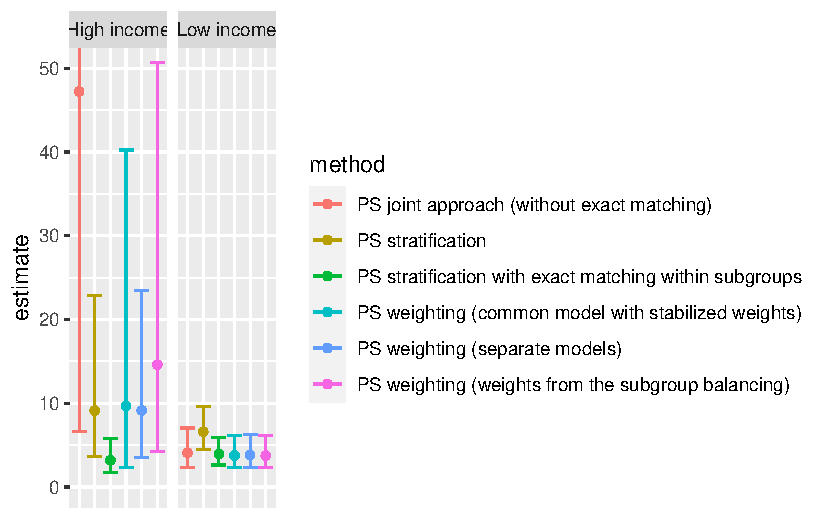
\includegraphics{chapter_07_files/figure-pdf/unnamed-chunk-53-1.pdf}

\hypertarget{version-info-2}{%
\section*{Version info}\label{version-info-2}}
\addcontentsline{toc}{section}{Version info}

\markright{Version info}

This chapter was rendered using the following version of R and its
packages:

\begin{verbatim}
R version 4.2.3 (2023-03-15 ucrt)
Platform: x86_64-w64-mingw32/x64 (64-bit)
Running under: Windows 10 x64 (build 19045)

Matrix products: default

locale:
[1] LC_COLLATE=Dutch_Netherlands.utf8  LC_CTYPE=Dutch_Netherlands.utf8   
[3] LC_MONETARY=Dutch_Netherlands.utf8 LC_NUMERIC=C                      
[5] LC_TIME=Dutch_Netherlands.utf8    

attached base packages:
[1] grid      stats     graphics  grDevices utils     datasets  methods  
[8] base     

other attached packages:
 [1] interactionR_0.1.6 simcausal_0.5.6    scales_1.2.1       ggplot2_3.4.2     
 [5] xtable_1.8-4       dplyr_1.1.2        kableExtra_1.3.4   knitr_1.43        
 [9] cowplot_1.1.1      readstata13_0.10.1 survey_4.2-1       survival_3.5-5    
[13] Matrix_1.5-4.1     broom_1.0.5        MatchIt_4.5.4      interactions_1.1.5
[17] jtools_2.2.1       sandwich_3.0-2     lmtest_0.9-40      zoo_1.8-12        
[21] optmatch_0.10.6    WeightIt_0.14.2    cobalt_4.5.1       table1_1.4.3      

loaded via a namespace (and not attached):
 [1] fontquiver_0.2.1        webshot_0.5.4           httr_1.4.6             
 [4] tools_4.2.3             backports_1.4.1         utf8_1.2.3             
 [7] R6_2.5.1                DBI_1.1.3               colorspace_2.1-0       
[10] withr_2.5.0             tidyselect_1.2.0        curl_5.0.1             
[13] compiler_4.2.3          textshaping_0.3.6       cli_3.6.1              
[16] rvest_1.0.3             expm_0.999-7            flextable_0.9.2        
[19] xml2_1.3.4              officer_0.6.2           fontBitstreamVera_0.1.1
[22] labeling_0.4.2          mvtnorm_1.2-2           askpass_1.1            
[25] systemfonts_1.0.4       stringr_1.5.0           digest_0.6.31          
[28] rmarkdown_2.22          svglite_2.1.1           gfonts_0.2.0           
[31] pkgconfig_2.0.3         htmltools_0.5.5         fastmap_1.1.1          
[34] rlang_1.1.1             rstudioapi_0.14         httpcode_0.3.0         
[37] shiny_1.7.4             farver_2.1.1            generics_0.1.3         
[40] jsonlite_1.8.5          car_3.1-2               zip_2.3.0              
[43] magrittr_2.0.3          Formula_1.2-5           Rcpp_1.0.10            
[46] munsell_0.5.0           fansi_1.0.4             abind_1.4-5            
[49] gdtools_0.3.3           lifecycle_1.0.3         chk_0.9.0              
[52] stringi_1.7.12          yaml_2.3.7              carData_3.0-5          
[55] promises_1.2.0.1        crayon_1.5.2            lattice_0.21-8         
[58] splines_4.2.3           pander_0.6.5            pillar_1.9.0           
[61] uuid_1.1-0              igraph_1.5.0            codetools_0.2-19       
[64] crul_1.4.0              glue_1.6.2              evaluate_0.21          
[67] msm_1.7                 mitools_2.4             fontLiberation_0.1.0   
[70] data.table_1.14.8       vctrs_0.6.3             httpuv_1.6.11          
[73] openssl_2.0.6           gtable_0.3.3            purrr_1.0.1            
[76] tidyr_1.3.0             assertthat_0.2.1        xfun_0.39              
[79] mime_0.12               later_1.3.1             ragg_1.2.5             
[82] viridisLite_0.4.2       tibble_3.2.1            ellipsis_0.3.2         
[85] rlemon_0.2.1           
\end{verbatim}

\bookmarksetup{startatroot}

\hypertarget{dealing-with-missing-data}{%
\chapter{Dealing with missing data}\label{dealing-with-missing-data}}

Johanna Munoz (Julius Center for Health Sciences and Primary Care)\\
Thomas Debray (Smart Data Analysis and Statistics B.V.)

\hfill\break

\hypertarget{main-analysis}{%
\section{Main Analysis}\label{main-analysis}}

The main objective of this analysis is to assess whether the number of
episodes (y) occurring within specific time periods (years) differs
between the treatment groups (1: DMF and 0: TERI). To address potential
confounding factors, the researchers consider variables such as patient
age, the log of premedical cost (\texttt{logPremedicalcost}), previous
DMT efficacy (\texttt{prevDMTefficacy}), and the number of episodes in
previous relapses (prerelapseNum).

When estimating treatment effects from observational data, an assumption
is made that the patient populations in both treatment groups are as
similar as possible. Various methods for balancing data across treatment
groups are proposed, including matching, inverse propensity weighting,
stratification, and regression adjustment.

In this case, the focus is specifically on the matching method, which
offers advantages over regression adjustment by potentially alleviating
issues related to model mis-specification. This includes addressing
non-linear relationships between certain confounders and the outcome
variable and accounting for treatment effects that may depend on
specific confounders (treatment-confounder interaction terms).
Propensity scores are used to match subjects in the treatment groups.

Moreover, intentionally introducing incomplete covariate variables in
this example adds complexity to the propensity score estimation.
Depending on the propensity score estimation technique employed, it may
be necessary to incorporate an imputation step. For instance, logistic
regression estimation requires complete data for all observations, while
XGBoost is robust to missing data \cite{zhao_propensity_2021}.

To estimate marginal treatment effects, the g-computation method is
employed \cite{snowden_implementation_2011}. This method involves
specifying a model for the outcome dependent on the treatment and
covariates. The potential outcomes, i.e., the predicted values of the
outcome on treatment (\(y_i^1\)) and control (\(y_i^0\)) for each sample
unit \(i\), are estimated. The marginal treatment effect is then
calculated by contrasting the averaged estimated potential outcomes.

In this example, we consider the estimation of comparative treatment
effects in the absence of treatment-effect heterogeneity.

\hypertarget{estimation-workflow}{%
\section{Estimation workflow}\label{estimation-workflow}}

The proposed workflow consists of the following steps:

\begin{figure}

{\centering 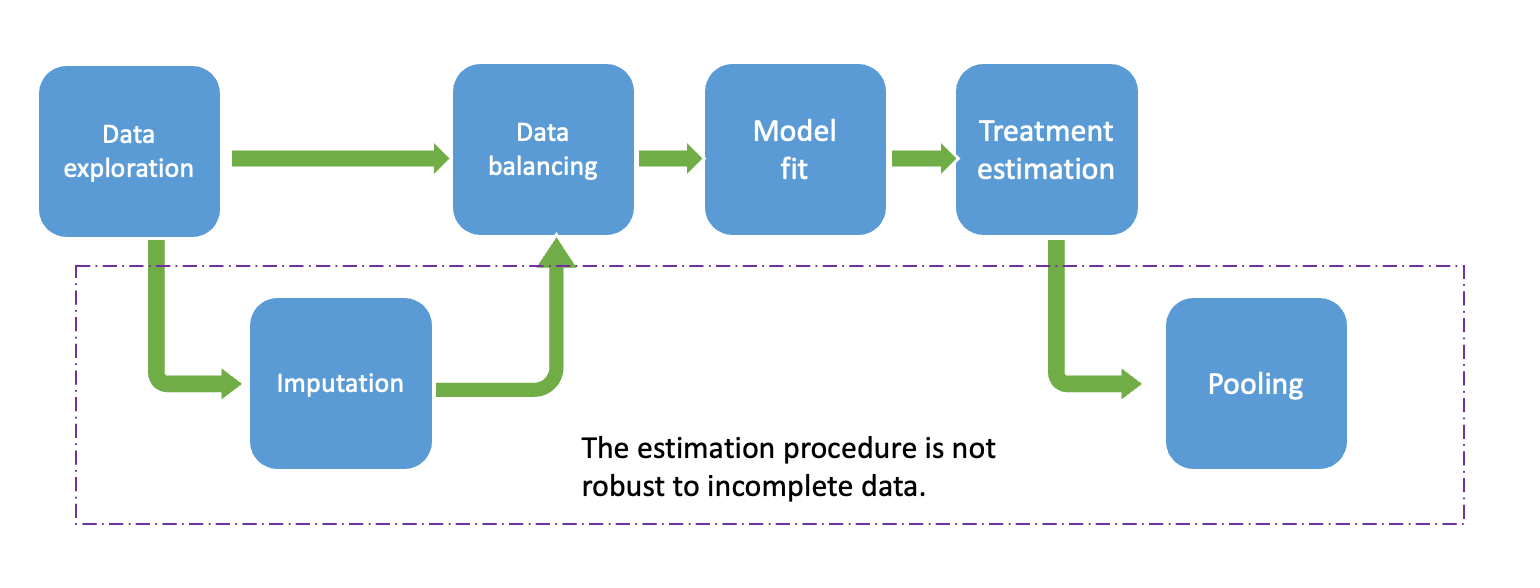
\includegraphics{resources/chapter 09/Workflow.png}

}

\caption{Estimation Workflow}

\end{figure}

\begin{enumerate}
\def\labelenumi{\arabic{enumi}.}
\tightlist
\item
  \textbf{Data Exploration:} In this step, we examine the observed data
  to comprehend the variables within the dataset. Our primary focus lies
  on identifying missing patterns and relationships among observed
  variables, including missing indicator variables and others. This
  exploration aids in discerning the most plausible missing mechanisms
  and suitable imputation techniques. Additionally, field experts'
  insights may be incorporated to enhance understanding of the missing
  process, potentially considering MNAR assumptions.
\item
  \textbf{Imputation:} It is essential to evaluate whether the
  imputation procedure is necessary or if simpler methods, such as
  complete case analysis, are more suitable. In case imputation
  procedures are required, selecting plausible imputation methods that
  align with the main model analysis is crucial. This involves choosing
  individual imputation methods for each incomplete variable,
  determining the predictor variables on the imputation model.
  Pre\_imputation (where imputation values can be deterministically
  derived from other variables) and Post-imputation (e.g.ensuring
  imputed values fall within a reasonable range) steps may also
  considered.
\item
  \textbf{Data Balancing:} Several methods, including PS matching or
  inverse weighting propensity score, can be utilized. It is required to
  evaluate the balance, which could be done via visual
  inspection.(eg.cobalt package). In this example, we estimate
  propensity scores using logistic regression. For most balancing
  procedures in R, counterparts specifically designed for imputed
  datasets are available, such as those in the matchthem R package,
  which includes PS matching and IPW as done in the matchit R package.
\item
  \textbf{Model Fit:} : It is fit a model to predict the outcomes for
  each sample unit under each possible treatment value (DMF and TERI),
  as predictors include the treatment and optionally the baseline
  covariates and also the propensity score.
\item
  \textbf{Treatment Estimation \& Pooling:} For simplicity in this
  tutorial, we will use the comparison functions from the R
  \textbf{matchingmethods} package \cite{arel_marginaleffects_2023},
  which can be used for completed data and also from outputs from the
  imputation process. In the last case, internally the functions
  calculate the treatment effects on each imputed dataset and pool the
  estimates using Rubin's Rules.
\end{enumerate}

Let's start by preparing the R environment. All the functions used in
this tutorial can be found in the resource file \texttt{functions.r}.

\begin{Shaded}
\begin{Highlighting}[]
\CommentTok{\# Load the required packages and additional functions}
\FunctionTok{source}\NormalTok{(}\StringTok{"resources/chapter 09/functions.r"}\NormalTok{) }
\end{Highlighting}
\end{Shaded}

\hypertarget{homogeneous-treatment-effect}{%
\section{Homogeneous Treatment
Effect}\label{homogeneous-treatment-effect}}

In this example, we focus on estimating comparative treatment effects in
the absence of heterogeneous treatment effects (HTE).

\hypertarget{generating-an-observational-dataset}{%
\subsection{Generating an Observational
Dataset}\label{generating-an-observational-dataset}}

We can simulate an observational dataset of \(N = 3000\) patients as
follows:

\begin{Shaded}
\begin{Highlighting}[]
\NormalTok{data\_hom }\OtherTok{\textless{}{-}} \FunctionTok{generate\_data}\NormalTok{(}\AttributeTok{n =} \DecValTok{3000}\NormalTok{, }\AttributeTok{seed =} \DecValTok{1234}\NormalTok{) }
\end{Highlighting}
\end{Shaded}

The \textbf{generate\_data()} function allows the specification of
various treatment effect options, easily adjustable by modifying the
beta parameter. In this instance, we assume a consistent treatment
effect across the entire target population. This dataset currently
contains no missing values.

The simulated dataset comprises two treatment groups with variations in
baseline characteristics. For example, the figure below illustrates
baseline imbalances in covariates such as age.

\begin{figure}

{\centering 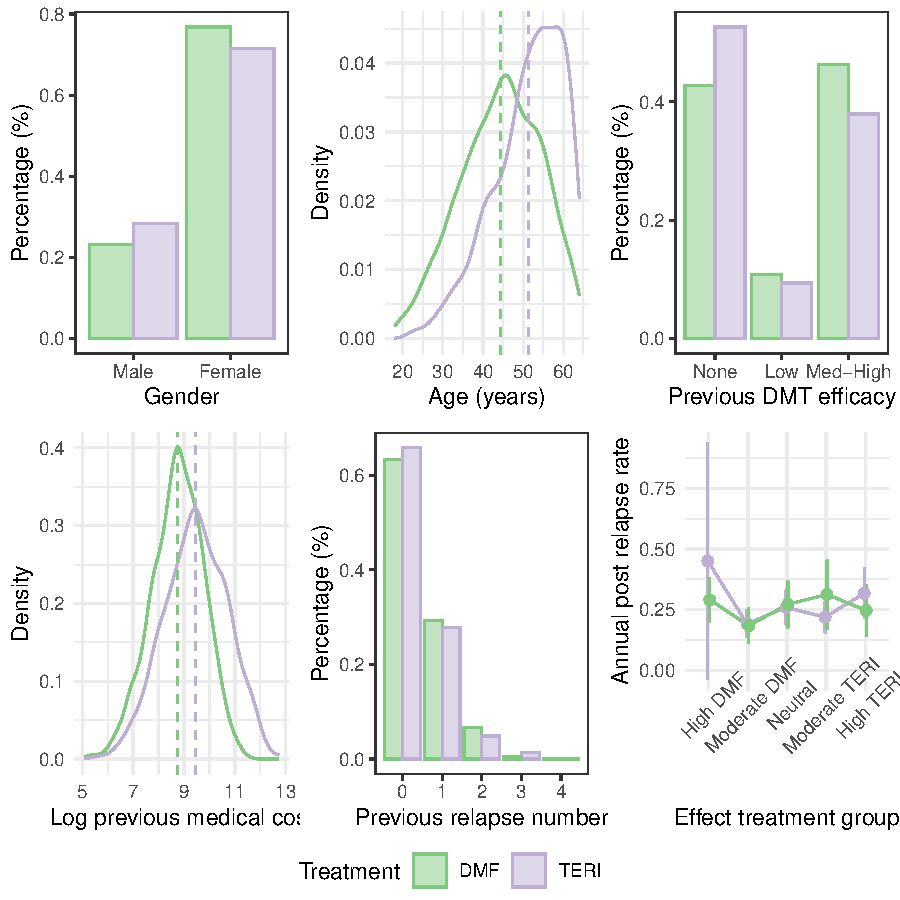
\includegraphics{chapter_09_files/figure-pdf/hom plotdata-1.pdf}

}

\caption{Figure 1:Distribution of confounders and outcome variable}

\end{figure}

We can calculate the treatment effect on the complete observed dataset.
To do this, we start by balancing the dataset using Propensity Score
matching. In this case, the propensity score model uses confounder
variables only: \texttt{age}, \texttt{gender}, \texttt{prevDMTefficacy},
\texttt{logPremedicalcost}, and \texttt{prerelapseNum}.

\begin{Shaded}
\begin{Highlighting}[]
\DocumentationTok{\#\# Apply Matching on the PS for the ATE}
\NormalTok{mF }\OtherTok{\textless{}{-}} \FunctionTok{matchit}\NormalTok{(  treatment }\SpecialCharTok{\textasciitilde{}}\NormalTok{ age }\SpecialCharTok{+}\NormalTok{ gender }\SpecialCharTok{+}\NormalTok{ prevDMTefficacy }\SpecialCharTok{+}\NormalTok{ logPremedicalcost }\SpecialCharTok{+}\NormalTok{ prerelapseNum, }
                \AttributeTok{data =}\NormalTok{ data\_hom,}
                \AttributeTok{family =}\NormalTok{ binomial,}
                \AttributeTok{method =} \StringTok{"full"}\NormalTok{,}
                \AttributeTok{caliper =} \FloatTok{0.2}\NormalTok{,}
                \AttributeTok{estimand =} \StringTok{"ATE"}\NormalTok{,}
                \AttributeTok{replace =} \ConstantTok{FALSE}\NormalTok{) }

\DocumentationTok{\#\# Extract matched data}
\NormalTok{mdata }\OtherTok{\textless{}{-}} \FunctionTok{match.data}\NormalTok{(mF)}
\end{Highlighting}
\end{Shaded}

Then, we proceed to model estimation. In this case, a Poisson model is
used with the form:

\[\begin{eqnarray}count_i\sim& Poisson(\lambda_i)\end{eqnarray}\]
\[\begin{eqnarray} log(\lambda_i) &=& \beta_0 + \beta_1treatment_i + \beta_2age + \beta_3gender \\ &+& \beta_4prevDMTefficacy + \beta_5logPremedicalcost
\\ &+& \beta_6prerelapseNum + \beta_7numSymptoms + offset(log(years)),\end{eqnarray}\]

Since patient measurements were recorded over varying time frames, the
natural logarithm of the years of evaluation is incorporated as an
offset in the model. The model is fitted with a glm function, and we
include the treatment and the baseline covariates as predictors, which
are optional if the data is well balanced. Additionally, it is necessary
to specify the matching weights in the glm function.

\begin{Shaded}
\begin{Highlighting}[]
\CommentTok{\# Model fit}
\NormalTok{fit\_mod }\OtherTok{\textless{}{-}} \FunctionTok{glm}\NormalTok{(}\FunctionTok{as.formula}\NormalTok{(}\StringTok{"y \textasciitilde{} treatment + gender + age + logPremedicalcost + prerelapseNum + prevDMTefficacy + numSymptoms + offset(log(years))"}\NormalTok{),}
                 \AttributeTok{family =} \FunctionTok{poisson}\NormalTok{(}\AttributeTok{link =} \StringTok{"log"}\NormalTok{),}
                 \AttributeTok{data =}\NormalTok{ mdata,}
                 \AttributeTok{weights =}\NormalTok{ weights)}
\end{Highlighting}
\end{Shaded}

Typically, Poisson models adjust standard errors using robust standard
errors to accommodate small values arising from the equidispersion
assumption. This correction can be directly applied to the model using
the vcovCL() function \cite{zeileis_sandwich_2022}. However, given that
we will calculate the treatment effect using the functions of the
\textbf{marginaleffects} package, this step becomes redundant. This
package allows specifying HC3 sandwich standard errors during treatment
estimation.

Finally, we calculate the Average Treatment Effect (ATE). The ATE is
defined as \[\tau_{ATE}=E(y_i^1-y_i^0)\]

But this cannot be directly extracted from the \(\beta_1\) parameter, as
the model has \(log(\lambda)\) as the response. We estimate it as:
\[\tau_{ATE}=E(\lambda^1_i-\lambda^0_i)\] This can be done with the
function \textbf{avg\_comparisons()}, from the R package marginaleffect,
that calculates the potential outcomes for each unit sample and then
combines them to summarize the average effect.

\begin{Shaded}
\begin{Highlighting}[]
\CommentTok{\# Estimation of treatment effects with robust standard errors}
\NormalTok{ATE }\OtherTok{\textless{}{-}} \FunctionTok{avg\_comparisons}\NormalTok{(fit\_mod, }
                       \AttributeTok{variables =} \FunctionTok{list}\NormalTok{(}\AttributeTok{treatment =} \FunctionTok{c}\NormalTok{(}\StringTok{"TERI"}\NormalTok{,}\StringTok{"DMF"}\NormalTok{)),}
                       \AttributeTok{vcov =} \StringTok{"HC3"}\NormalTok{,}
                       \AttributeTok{newdata =}\NormalTok{ mdata,}
                       \AttributeTok{wts =} \StringTok{"weights"}\NormalTok{)}

\NormalTok{result\_ATE }\OtherTok{\textless{}{-}} \FunctionTok{data.frame}\NormalTok{( ATE,}
                          \AttributeTok{analysis =} \StringTok{"Full Data"}\NormalTok{)}
\end{Highlighting}
\end{Shaded}

Henceforth, for ease of explanation, we will use the function
\textbf{TE\_estimation()} attached to the function code that performs
all the previous estimation steps at once.

\hypertarget{version-info-3}{%
\section*{Version info}\label{version-info-3}}
\addcontentsline{toc}{section}{Version info}

\markright{Version info}

This chapter was rendered using the following version of R and its
packages:

\begin{verbatim}
R version 4.2.3 (2023-03-15 ucrt)
Platform: x86_64-w64-mingw32/x64 (64-bit)
Running under: Windows 10 x64 (build 19045)

Matrix products: default

locale:
[1] LC_COLLATE=Dutch_Netherlands.utf8  LC_CTYPE=Dutch_Netherlands.utf8   
[3] LC_MONETARY=Dutch_Netherlands.utf8 LC_NUMERIC=C                      
[5] LC_TIME=Dutch_Netherlands.utf8    

attached base packages:
[1] grid      stats     graphics  grDevices utils     datasets  methods  
[8] base     

other attached packages:
 [1] marginaleffects_0.15.0 ggplot2_3.4.3          missForest_1.5        
 [4] sandwich_3.0-2         PSweight_1.1.8         cobalt_4.5.1          
 [7] WeightIt_0.14.2        MatchIt_4.5.4          optmatch_0.10.6       
[10] truncnorm_1.0-9        MASS_7.3-60            survey_4.2-1          
[13] survival_3.5-5         Matrix_1.5-4.1         data.table_1.14.8     
[16] tidyr_1.3.0            MatchThem_1.1.0        ggmice_0.1.0          
[19] dplyr_1.1.2            mice_3.16.0            table1_1.4.3          
[22] kableExtra_1.3.4      

loaded via a namespace (and not attached):
 [1] nlme_3.1-162          webshot_0.5.5         httr_1.4.7           
 [4] numDeriv_2016.8-1.1   doRNG_1.8.6           tools_4.2.3          
 [7] backports_1.4.1       utf8_1.2.3            R6_2.5.1             
[10] rpart_4.1.19          DBI_1.1.3             colorspace_2.1-0     
[13] jomo_2.7-6            nnet_7.3-19           withr_2.5.0          
[16] gbm_2.1.8.1           tidyselect_1.2.0      compiler_4.2.3       
[19] glmnet_4.1-7          cli_3.6.1             rvest_1.0.3          
[22] xml2_1.3.4            scales_1.2.1          nnls_1.5             
[25] randomForest_4.7-1.1  systemfonts_1.0.4     stringr_1.5.0        
[28] digest_0.6.31         minqa_1.2.5           rmarkdown_2.24       
[31] svglite_2.1.1         pkgconfig_2.0.3       htmltools_0.5.5      
[34] lme4_1.1-33           itertools_0.1-3       fastmap_1.1.1        
[37] rlang_1.1.1           rstudioapi_0.15.0     shape_1.4.6          
[40] generics_0.1.3        zoo_1.8-12            jsonlite_1.8.5       
[43] magrittr_2.0.3        Formula_1.2-5         Rcpp_1.0.10          
[46] munsell_0.5.0         fansi_1.0.4           lifecycle_1.0.3      
[49] stringi_1.7.12        yaml_2.3.7            parallel_4.2.3       
[52] mitml_0.4-5           crayon_1.5.2          lattice_0.21-8       
[55] splines_4.2.3         knitr_1.44            pillar_1.9.0         
[58] boot_1.3-28.1         rngtools_1.5.2        codetools_0.2-19     
[61] pan_1.6               glue_1.6.2            evaluate_0.21        
[64] mitools_2.4           vctrs_0.6.3           nloptr_2.0.3         
[67] foreach_1.5.2         gtable_0.3.4          purrr_1.0.1          
[70] xfun_0.39             SuperLearner_2.0-28.1 broom_1.0.5          
[73] viridisLite_0.4.2     tibble_3.2.1          iterators_1.0.14     
[76] gam_1.22-2           
\end{verbatim}

\bookmarksetup{startatroot}

\hypertarget{systematic-review-and-meta-analysis-of-real-world-evidence}{%
\chapter{Systematic review and meta-analysis of Real-World
Evidence}\label{systematic-review-and-meta-analysis-of-real-world-evidence}}

Dimitris Mavridis (University of Ioannina)\\
Thomas Debray (Smart Data Analysis and Statistics B.V.)

\hfill\break

\hypertarget{introduction-1}{%
\section{Introduction}\label{introduction-1}}

We first load the required packages

\begin{Shaded}
\begin{Highlighting}[]
\FunctionTok{library}\NormalTok{(dplyr)}
\FunctionTok{library}\NormalTok{(gemtc)}
\FunctionTok{library}\NormalTok{(netmeta)}
\end{Highlighting}
\end{Shaded}

\hypertarget{pairwise-meta-analysis-of-clinical-trials}{%
\section{Pairwise meta-analysis of clinical
trials}\label{pairwise-meta-analysis-of-clinical-trials}}

\hypertarget{toculizumab-for-coronavirus-disease-2019}{%
\subsection{Toculizumab for coronavirus disease
2019}\label{toculizumab-for-coronavirus-disease-2019}}

In this example, we consider the results from a systematic literature
review of clinical trials investigating any pharmacological in
hosptialized patients with coronavirus disease 2019 (Selvarajan et al.
2022). A total of 23 randomized controlled trials were included and
studied seven different interventions: dexamethasone, remdesivir,
tocilizumab, hydroxychloroquine, combination of lopinavir/ritonavir,
favipiravir and interferon-β. We here focus on the synthesis of 7 trials
that comparted toculizumab (\texttt{TOCI}) to standard care
(\texttt{STD}) and collected mortality data.

\begin{longtable*}{lrrrrrr}
\toprule
studlab & treat1 & treat2 & event1 & n1 & event2 & n2\\
\midrule
\endfirsthead
\multicolumn{7}{@{}l}{\textit{(continued)}}\\
\toprule
studlab & treat1 & treat2 & event1 & n1 & event2 & n2\\
\midrule
\endhead

\endfoot
\bottomrule
\endlastfoot
Hermine et al & TOCI & STD & 7 & 63 & 8 & 67\\
Rosas et al & TOCI & STD & 58 & 294 & 28 & 144\\
Salama et al & TOCI & STD & 26 & 249 & 11 & 128\\
Salvarini et al & TOCI & STD & 2 & 60 & 1 & 66\\
Stone et al & TOCI & STD & 9 & 161 & 3 & 82\\
Veiga et al & TOCI & STD & 14 & 65 & 6 & 64\\*
\end{longtable*}

We now conduct a pairwise meta-analysis to assess the pooled effect of
tocilizumab versus standard care. For each study, the log odds ratio and
corresponding standard error is derived after which the corresponding
estimates are pooled using the Mantel-Haenszel method.

\begin{Shaded}
\begin{Highlighting}[]
\NormalTok{results.TOCI }\OtherTok{\textless{}{-}} \FunctionTok{metabin}\NormalTok{(event1,n1,event2,n2,studlab,}\AttributeTok{data=}\NormalTok{tocilizumab,}
                        \AttributeTok{sm=}\StringTok{"OR"}\NormalTok{,}\AttributeTok{main=}\StringTok{"tocilizumab vs standard care"}\NormalTok{, }
                        \AttributeTok{prediction=}\ConstantTok{TRUE}\NormalTok{)}
\FunctionTok{forest}\NormalTok{(results.TOCI, }\AttributeTok{leftcols =} \StringTok{"studlab"}\NormalTok{, }\AttributeTok{rightcols =} \StringTok{"effect.ci"}\NormalTok{)}
\end{Highlighting}
\end{Shaded}

\begin{figure}[H]

{\centering 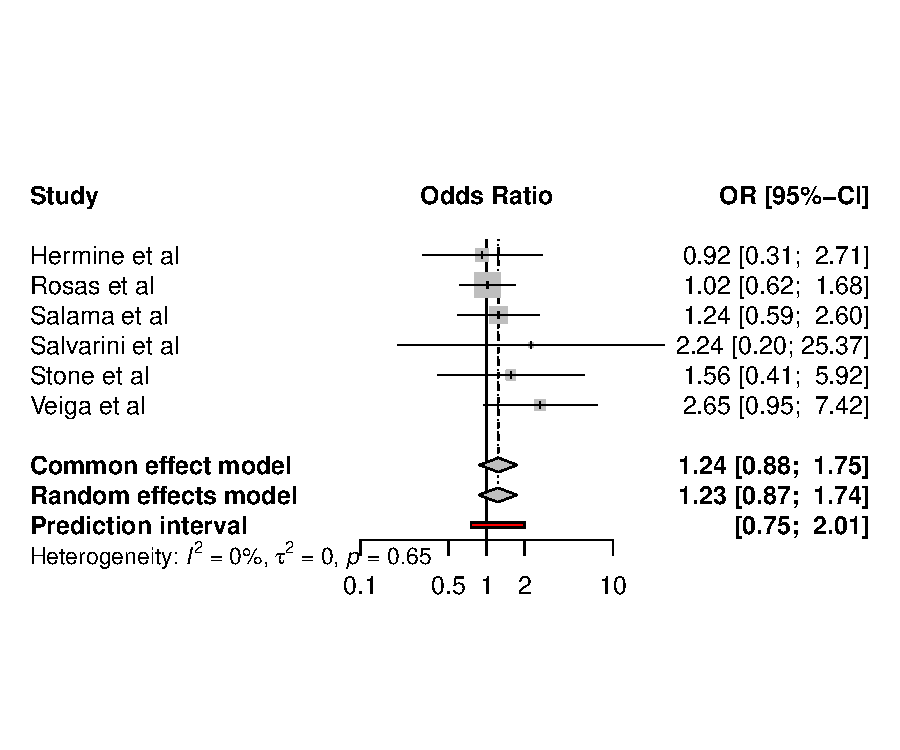
\includegraphics{chapter_10_files/figure-pdf/unnamed-chunk-6-1.pdf}

}

\end{figure}

Altough a random effects meta-analysis was conducted, no heterogeneity
was found (\(\tau\)=0, with a 95\% confidence interval ranging from 0 to
0.85).

\hypertarget{remdesivir-for-coronavirus-disease-2019}{%
\subsection{Remdesivir for coronavirus disease
2019}\label{remdesivir-for-coronavirus-disease-2019}}

In aforementioned example, a total of 4 trials compared remdesivir to
standard care:

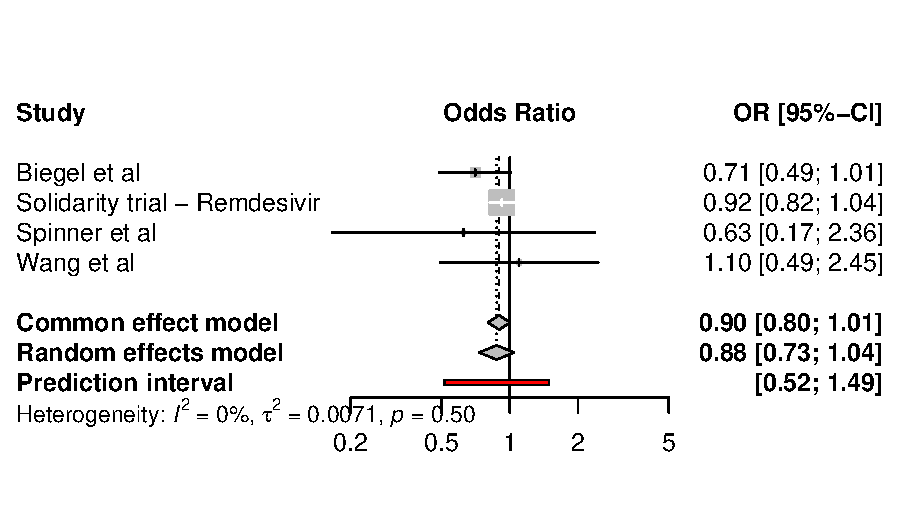
\includegraphics{chapter_10_files/figure-pdf/unnamed-chunk-7-1.pdf}

\hypertarget{network-meta-analysis-of-clinical-trials}{%
\section{Network meta-analysis of clinical
trials}\label{network-meta-analysis-of-clinical-trials}}

We here use the R packages \texttt{netmeta} for conducting a frequentist
network meta-analysis. A detailed tutorial on the use of
\texttt{netmeta} is available from the book
\href{https://bookdown.org/MathiasHarrer/Doing_Meta_Analysis_in_R/}{Doing
Meta-Analysis with R: A Hands-On Guide}.

\hypertarget{interventions-for-coronavirus-disease-2019}{%
\subsection{Interventions for coronavirus disease
2019}\label{interventions-for-coronavirus-disease-2019}}

We here consider data from a study which aimed to assess the comparative
effectiveness of remdesivir and tocilizumab for reducing mortality in
hospitalised COVID-19 patients. 80 trials were identified from two
published network meta-analyses (Selvarajan et al. 2022), (Siemieniuk et
al. 2020), a living COVID-19 trial database (COVID-NMA Initiative)
{[}Covid-NMA.com{]}, and a clinical trial database
{[}clinicaltrials.gov{]}. Trials were included in this study if the
patient population included hospitalized COVID-19 patients, active
treatment was remdesivir or tocilizumab, comparator treatment was
placebo or standard care, short-term mortality data was available, and
the trial was published. 21 trials were included. For included trials, a
risk of bias score was extracted from the COVID-NMA Initiative.

\begin{longtable*}{lrrrrrr}
\toprule
studlab & treat1 & treat2 & event1 & n1 & event2 & n2\\
\midrule
\endfirsthead
\multicolumn{7}{@{}l}{\textit{(continued)}}\\
\toprule
studlab & treat1 & treat2 & event1 & n1 & event2 & n2\\
\midrule
\endhead

\endfoot
\bottomrule
\endlastfoot
Ader & REM & STD & 34 & 414 & 37 & 418\\
Beigel (ACTT-1) & REM & STD & 59 & 541 & 77 & 521\\
Broman & TOCI & STD & 1 & 57 & 0 & 29\\
Criner & REM & STD & 4 & 384 & 4 & 200\\
Declerq (COV-AID) & TOCI & STD & 10 & 81 & 9 & 74\\
Gordon (REMAP-CAP) & TOCI & STD & 83 & 353 & 116 & 358\\
Hermine (CORIMUNO) & TOCI & STD & 7 & 63 & 8 & 67\\
Horby (RECOVERY) & TOCI & STD & 621 & 2022 & 729 & 2094\\
Islam & REM & STD & 0 & 30 & 0 & 30\\
Mahajan & REM & STD & 5 & 34 & 3 & 36\\
Pan (WHO Solidarity) & REM & STD & 602 & 4146 & 643 & 4129\\
Rosas (COVACTA) & TOCI & STD & 58 & 294 & 28 & 144\\
Rutgers & TOCI & STD & 21 & 174 & 34 & 180\\
Salama (EMPACTA) & TOCI & STD & 26 & 249 & 11 & 128\\
Salvarani & TOCI & STD & 2 & 60 & 1 & 63\\
Soin (COVINTOC) & TOCI & STD & 11 & 92 & 15 & 88\\
Spinner & REM & STD & 5 & 384 & 4 & 200\\
Stone (BACC-BAY) & TOCI & STD & 9 & 161 & 4 & 82\\
Talaschian & TOCI & STD & 5 & 17 & 4 & 19\\
Veiga (TOCIBRAS) & TOCI & STD & 14 & 65 & 6 & 64\\
Wang & REM & STD & 22 & 158 & 10 & 78\\*
\end{longtable*}

The corresponding network is displayed below:

\begin{figure}

{\centering 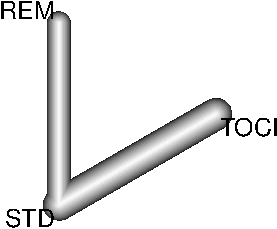
\includegraphics{chapter_10_files/figure-pdf/unnamed-chunk-9-1.pdf}

}

\caption{Evidence network of the 21 coronavirus-19 trials}

\end{figure}

We use the following command to calculate the log odds ratios and
corresponding standard errors for each study:

\begin{Shaded}
\begin{Highlighting}[]
\NormalTok{covid }\OtherTok{\textless{}{-}} \FunctionTok{pairwise}\NormalTok{(}\AttributeTok{treat =}\NormalTok{ treat, }\AttributeTok{event =}\NormalTok{ event, }\AttributeTok{n =}\NormalTok{ n, }\AttributeTok{studlab =}\NormalTok{ studlab, }\AttributeTok{sm =} \StringTok{"OR"}\NormalTok{)}
\FunctionTok{head}\NormalTok{(covid)}
\end{Highlighting}
\end{Shaded}

\begin{tabular}{r|r|l|l|l|r|r|r|r|r|l}
\hline
TE & seTE & studlab & treat1 & treat2 & event1 & n1 & event2 & n2 & incr & allstudies\\
\hline
-0.0819293 & 0.2483849 & Ader & REM & STD & 34 & 414 & 37 & 418 & 0.0 & FALSE\\
\hline
-0.3483875 & 0.1851030 & Beigel (ACTT-1) & REM & STD & 59 & 541 & 77 & 521 & 0.0 & FALSE\\
\hline
0.4487619 & 1.6487159 & Broman & TOCI & STD & 1 & 57 & 0 & 29 & 0.5 & FALSE\\
\hline
-0.6620566 & 0.7125543 & Criner & REM & STD & 4 & 384 & 4 & 200 & 0.0 & FALSE\\
\hline
0.0170679 & 0.4904898 & Declerq (COV-AID) & TOCI & STD & 10 & 81 & 9 & 74 & 0.0 & FALSE\\
\hline
-0.4442338 & 0.1688337 & Gordon (REMAP-CAP) & TOCI & STD & 83 & 353 & 116 & 358 & 0.0 & FALSE\\
\hline
\end{tabular}

Below, we conduct a random effects network meta-analysis where we
consider standard care (\texttt{STD}) as the control treatment. Note
that we have one study where zero cell counts occur, this study will not
contribute to the NMA as the log odds ratio and its standard error
cannot be determined.

\begin{Shaded}
\begin{Highlighting}[]
\NormalTok{NMA.covid }\OtherTok{\textless{}{-}} \FunctionTok{netmeta}\NormalTok{(}\AttributeTok{TE =}\NormalTok{ TE, }\AttributeTok{seTE =}\NormalTok{ seTE, }\AttributeTok{treat1 =}\NormalTok{ treat1, }\AttributeTok{treat2 =}\NormalTok{ treat2,}
                     \AttributeTok{studlab =}\NormalTok{ studlab, }\AttributeTok{data =}\NormalTok{ covid, }\AttributeTok{sm =} \StringTok{"OR"}\NormalTok{, }\AttributeTok{ref =} \StringTok{"STD"}\NormalTok{,}
                     \AttributeTok{comb.random =} \ConstantTok{TRUE}\NormalTok{, }\AttributeTok{common =} \ConstantTok{FALSE}\NormalTok{, }\AttributeTok{warn =} \ConstantTok{FALSE}\NormalTok{)}
\NormalTok{NMA.covid }
\end{Highlighting}
\end{Shaded}

\begin{verbatim}
Number of studies: k = 20
Number of pairwise comparisons: m = 20
Number of treatments: n = 3
Number of designs: d = 2

Random effects model

Treatment estimate (sm = 'OR', comparison: other treatments vs 'STD'):
         OR           95%-CI     z p-value
REM  0.8999 [0.8067; 1.0039] -1.89  0.0588
STD       .                .     .       .
TOCI 0.8301 [0.7434; 0.9268] -3.31  0.0009

Quantifying heterogeneity / inconsistency:
tau^2 = 0; tau = 0; I^2 = 0% [0.0%; 48.9%]

Tests of heterogeneity (within designs) and inconsistency (between designs):
                    Q d.f. p-value
Total           16.38   18  0.5663
Within designs  16.38   18  0.5663
Between designs  0.00    0      --
\end{verbatim}

A league table of the treatment effect estimates is given below:

\begin{Shaded}
\begin{Highlighting}[]
\FunctionTok{netleague}\NormalTok{(NMA.covid)}
\end{Highlighting}
\end{Shaded}

\begin{verbatim}
League table (random effects model):
                                                                        
                     REM 0.8999 [0.8067; 1.0039]                       .
 0.8999 [0.8067; 1.0039]                     STD 1.2047 [1.0789; 1.3451]
 1.0842 [0.9282; 1.2663] 1.2047 [1.0789; 1.3451]                    TOCI
\end{verbatim}

We can also present the results in a forest plot:

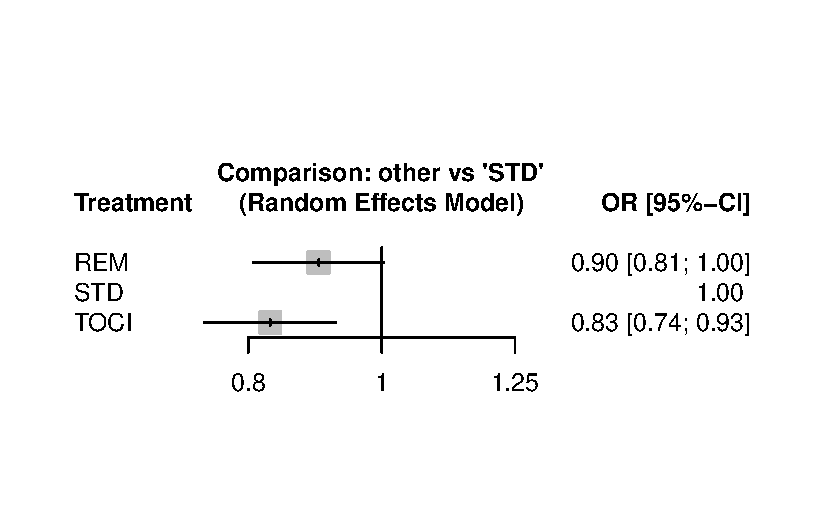
\includegraphics{chapter_10_files/figure-pdf/unnamed-chunk-14-1.pdf}

The figure below shows the percentage of direct and indirect evidence
used for each estimated comparison.

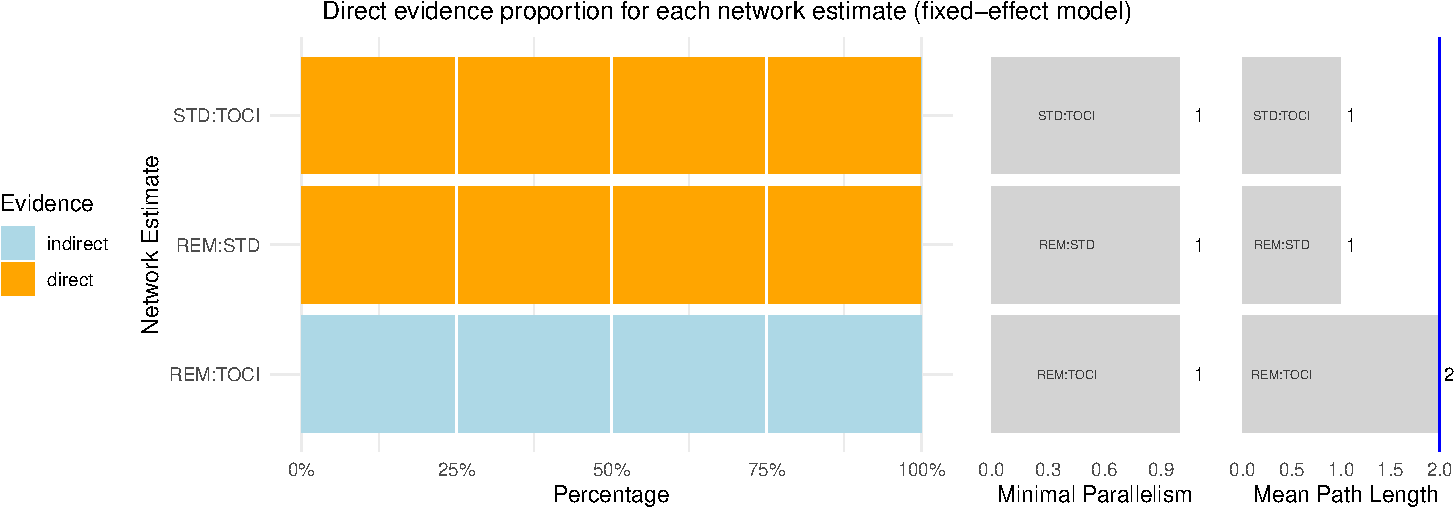
\includegraphics{chapter_10_files/figure-pdf/unnamed-chunk-15-1.pdf}

We now consider a Bayesian random effects network meta-analysis that
analyzes the observed event counts using a binomial link function.

\begin{Shaded}
\begin{Highlighting}[]
\NormalTok{bdata }\OtherTok{\textless{}{-}} \FunctionTok{data.frame}\NormalTok{(}\AttributeTok{study =}\NormalTok{ studlab,}
                    \AttributeTok{treatment =}\NormalTok{ treat,}
                    \AttributeTok{responders =}\NormalTok{ event,}
                    \AttributeTok{sampleSize =}\NormalTok{ n)}

\NormalTok{network }\OtherTok{\textless{}{-}} \FunctionTok{mtc.network}\NormalTok{(}\AttributeTok{data.ab  =}\NormalTok{ bdata)}

\NormalTok{model }\OtherTok{\textless{}{-}} \FunctionTok{mtc.model}\NormalTok{(network,}
                   \AttributeTok{likelihood =} \StringTok{"binom"}\NormalTok{,}
                   \AttributeTok{link =} \StringTok{"log"}\NormalTok{,}
                   \AttributeTok{linearModel =} \StringTok{"random"}\NormalTok{,}
                   \AttributeTok{n.chain =} \DecValTok{3}\NormalTok{)}
\end{Highlighting}
\end{Shaded}

\begin{Shaded}
\begin{Highlighting}[]
\CommentTok{\# Adaptation}
\NormalTok{mcmc1 }\OtherTok{\textless{}{-}} \FunctionTok{mtc.run}\NormalTok{(model, }\AttributeTok{n.adapt =} \DecValTok{1000}\NormalTok{, }\AttributeTok{n.iter =} \DecValTok{1000}\NormalTok{, }\AttributeTok{thin =} \DecValTok{10}\NormalTok{)}
\end{Highlighting}
\end{Shaded}

\begin{verbatim}
Compiling model graph
   Resolving undeclared variables
   Allocating nodes
Graph information:
   Observed stochastic nodes: 42
   Unobserved stochastic nodes: 45
   Total graph size: 930

Initializing model
\end{verbatim}

\begin{Shaded}
\begin{Highlighting}[]
\CommentTok{\# Sampling}
\NormalTok{mcmc2 }\OtherTok{\textless{}{-}} \FunctionTok{mtc.run}\NormalTok{(model, }\AttributeTok{n.adapt =} \DecValTok{10000}\NormalTok{, }\AttributeTok{n.iter =} \DecValTok{100000}\NormalTok{, }\AttributeTok{thin =} \DecValTok{10}\NormalTok{)}
\end{Highlighting}
\end{Shaded}

\begin{verbatim}
Compiling model graph
   Resolving undeclared variables
   Allocating nodes
Graph information:
   Observed stochastic nodes: 42
   Unobserved stochastic nodes: 45
   Total graph size: 930

Initializing model
\end{verbatim}

We can extract the pooled treatment effect estimates from the posterior
distribution. When using \texttt{STD} as control group, we have:

\begin{Shaded}
\begin{Highlighting}[]
\FunctionTok{summary}\NormalTok{(}\FunctionTok{relative.effect}\NormalTok{(mcmc2, }\AttributeTok{t1 =} \StringTok{"STD"}\NormalTok{))}
\end{Highlighting}
\end{Shaded}

\begin{verbatim}

Results on the Log Risk Ratio scale

Iterations = 10010:110000
Thinning interval = 10 
Number of chains = 3 
Sample size per chain = 10000 

1. Empirical mean and standard deviation for each variable,
   plus standard error of the mean:

              Mean      SD  Naive SE Time-series SE
d.STD.REM  -0.1075 0.09755 0.0005632      0.0008145
d.STD.TOCI -0.1126 0.08254 0.0004765      0.0008494
sd.d        0.1129 0.08934 0.0005158      0.0016915

2. Quantiles for each variable:

                2.5%      25%      50%      75%   97.5%
d.STD.REM  -0.317752 -0.15982 -0.10226 -0.05105 0.08262
d.STD.TOCI -0.256122 -0.16379 -0.12024 -0.06997 0.07558
sd.d        0.005699  0.04386  0.09278  0.15994 0.33299
\end{verbatim}

The corresponding odds ratios are as follows:

\begin{longtable*}{lc}
\toprule
Comparison & 95\% CrI\\
\midrule
REM vs. STD & 0.9 (0.73; 1.09)\\
TOCI vs. STD & 0.89 (0.77; 1.08)\\
REM vs. TOCI & 1.02 (0.75; 1.27)\\
\bottomrule
\end{longtable*}

Finally, we expand the COVID-19 network with trials investigating the
effectiveness of hydroxychloroquine (HCQ), lopinavir/ritonavir (LOPI),
dexamethasone (DEXA) or interferon-\(\beta\) (INTB) (Selvarajan et al.
2022). The corresponding network is displayed below:

\begin{figure}

{\centering 
\includegraphics{chapter_10_files/figure-pdf/unnamed-chunk-20-1.pdf}

}

\caption{Evidence network of the 33 coronavirus-19 trials}

\end{figure}

We conducted a random effects network meta-analysis, results are
depicted below:

\begin{verbatim}
Number of studies: k = 33
Number of pairwise comparisons: m = 33
Number of treatments: n = 7
Number of designs: d = 6

Random effects model

Treatment estimate (sm = 'OR', comparison: other treatments vs 'STD'):
         OR           95%-CI     z p-value            95%-PI
DEXA 0.8557 [0.7558; 0.9688] -2.46  0.0139  [0.7463; 0.9812]
HCQ  1.1809 [0.8934; 1.5610]  1.17  0.2428  [0.8786; 1.5872]
INTB 1.1606 [0.9732; 1.3841]  1.66  0.0973  [0.9604; 1.4026]
LOPI 1.0072 [0.8906; 1.1392]  0.11  0.9085  [0.8794; 1.1537]
REM  0.8983 [0.8014; 1.0070] -1.84  0.0658  [0.7913; 1.0199]
STD       .                .     .       .                 .
TOCI 0.8304 [0.7410; 0.9306] -3.20  0.0014  [0.7316; 0.9426]

Quantifying heterogeneity / inconsistency:
tau^2 = 0.0004; tau = 0.0205; I^2 = 0.6% [0.0%; 42.3%]

Tests of heterogeneity (within designs) and inconsistency (between designs):
                    Q d.f. p-value
Total           27.18   27  0.4543
Within designs  27.18   27  0.4543
Between designs  0.00    0      --
\end{verbatim}

We can calculate the P score for each treatment as follows:

\begin{Shaded}
\begin{Highlighting}[]
\FunctionTok{netrank}\NormalTok{(NMA.covidf)}
\end{Highlighting}
\end{Shaded}

\begin{verbatim}
     P-score
TOCI  0.9070
DEXA  0.8357
REM   0.7143
STD   0.4027
LOPI  0.3899
HCQ   0.1336
INTB  0.1166
\end{verbatim}

\hypertarget{pharmacologic-treatments-for-chronic-obstructive-pulmonary-disease}{%
\subsection{Pharmacologic treatments for chronic obstructive pulmonary
disease}\label{pharmacologic-treatments-for-chronic-obstructive-pulmonary-disease}}

In this example, we consider the resuls from a systematic review of
randomized controlled trials on pharmacologic treatments for chronic
obstructive pulmonary disease (Baker, Baker, and Coleman 2009). The
primary outcome, occurrence of one or more episodes of COPD
exacerbation, is binary (yes / no). For this outcome, five drug
treatments (fluticasone, budesonide, salmeterol, formoterol, tiotropium)
and two combinations (fluticasone + salmeterol, budesonide + formoterol)
were compared to placebo. The authors considered the two combinations as
separate treatments instead of evaluating the individual components.

\begin{Shaded}
\begin{Highlighting}[]
\FunctionTok{data}\NormalTok{(Baker2009)}
\end{Highlighting}
\end{Shaded}

\begin{tabular}{l|r|r|l|r|r}
\hline
study & year & id & treatment & exac & total\\
\hline
Llewellyn-Jones 1996 & 1996 & 1 & Fluticasone & 0 & 8\\
\hline
Llewellyn-Jones 1996 & 1996 & 1 & Placebo & 3 & 8\\
\hline
Boyd 1997 & 1997 & 2 & Salmeterol & 47 & 229\\
\hline
Boyd 1997 & 1997 & 2 & Placebo & 59 & 227\\
\hline
Paggiaro 1998 & 1998 & 3 & Fluticasone & 45 & 142\\
\hline
Paggiaro 1998 & 1998 & 3 & Placebo & 51 & 139\\
\hline
\end{tabular}

\begin{Shaded}
\begin{Highlighting}[]
\NormalTok{Baker }\OtherTok{\textless{}{-}} \FunctionTok{pairwise}\NormalTok{(}\AttributeTok{treat =}\NormalTok{ treatment,}
                  \AttributeTok{event =}\NormalTok{ exac,}
                  \AttributeTok{n =}\NormalTok{ total,}
                  \AttributeTok{studlab =}\NormalTok{ id,}
                  \AttributeTok{sm =} \StringTok{"OR"}\NormalTok{,}
                  \AttributeTok{data =}\NormalTok{ Baker2009)}

\NormalTok{NMA.COPD }\OtherTok{\textless{}{-}} \FunctionTok{netmeta}\NormalTok{(}\AttributeTok{TE =}\NormalTok{ TE, }\AttributeTok{seTE =}\NormalTok{ seTE, }\AttributeTok{treat1 =}\NormalTok{ treat1, }\AttributeTok{treat2 =}\NormalTok{ treat2,}
                    \AttributeTok{studlab =}\NormalTok{ studlab, }\AttributeTok{data =}\NormalTok{ Baker, }\AttributeTok{sm=}\StringTok{"OR"}\NormalTok{, }\AttributeTok{ref =} \StringTok{"Placebo"}\NormalTok{,}
                    \AttributeTok{comb.random =} \ConstantTok{TRUE}\NormalTok{)}
\end{Highlighting}
\end{Shaded}

\begin{verbatim}
Warning: Comparisons with missing TE / seTE or zero seTE not considered in
network meta-analysis.
\end{verbatim}

\begin{verbatim}
Comparisons not considered in network meta-analysis:
 studlab                 treat1     treat2 TE seTE
      39 Fluticasone+Salmeterol    Placebo NA   NA
      39 Fluticasone+Salmeterol Salmeterol NA   NA
      39             Salmeterol    Placebo NA   NA
\end{verbatim}

\begin{Shaded}
\begin{Highlighting}[]
\FunctionTok{netgraph}\NormalTok{(NMA.COPD)}
\end{Highlighting}
\end{Shaded}

\begin{figure}[H]

{\centering 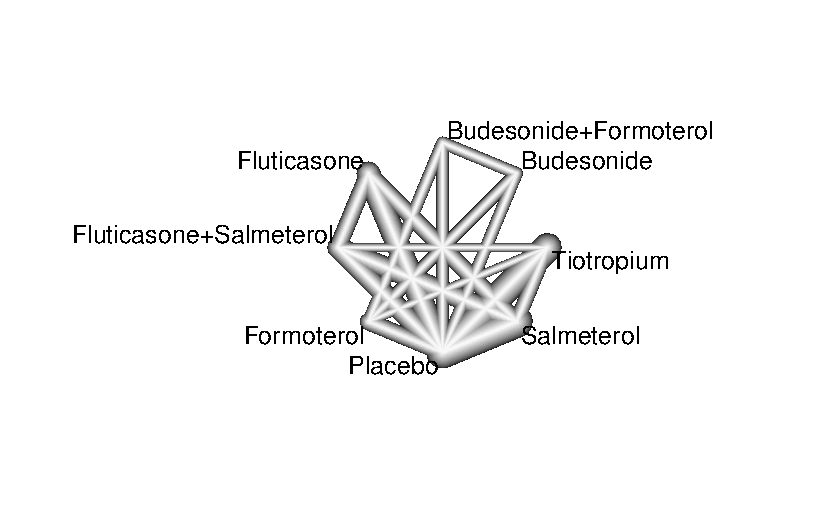
\includegraphics{chapter_10_files/figure-pdf/unnamed-chunk-25-1.pdf}

}

\end{figure}

\hypertarget{advanced-therapies-for-ulcerative-colitis}{%
\subsection{Advanced Therapies for Ulcerative
Colitis}\label{advanced-therapies-for-ulcerative-colitis}}

In this example, we consider a systematic literature review of Phase 3
randomized controlled trials investigating the following advanced
therapies: infliximab, adalimumab, vedolizumab, golimumab, tofacitinib,
ustekinumab, filgotinib, ozanimod, and upadacitinib (Panaccione et al.
2023). This review included 48 RCTs, from which 23 were found eligible
for inclusion in a network meta-analysis. The included RCT populations
were largely comparable in their baseline characteristics, though some
heterogeneity was noted in weight, disease duration, extent of disease,
and concomitant medications. A risk of bias assessment showed a low risk
of bias for all included RCTs, which were all industry sponsored.

We here focus on the synthesis of 18 trials that contributed efficacy
data for induction in bio-naive populations. The following FDA- and/or
EMA-approved biologic or SMD doses were investigated:

\begin{itemize}
\tightlist
\item
  Adalimumab subcutaneous 160 mg at week 0, 80 mg at week 2, and 40 mg
  at week 4 (\texttt{ADA160/80})
\item
  Infliximab intravenous 5 mg/kg (\texttt{INF5}) at weeks 0, 2, and 6
  then every 8 weeks
\item
  Infliximab intravenous 10 mg/kg (\texttt{INF10}) at weeks 0, 2, and 6
  then every 8 weeks
\item
  Filgotinib oral 100 mg once daily (\texttt{FIL100})
\item
  Filgotinib oral 200 mg once daily (\texttt{FIL200})
\item
  Golimumab subcutaneous 200 mg at week 0 and 100 mg at week 2
  (\texttt{GOL200/100})
\item
  Ozanimod oral 0.23 mg once daily for 4 days, 0.46 mg once daily for 3
  days, then 0.92 mg once daily (\texttt{OZA0.92})
\item
  Tofacitinib oral 10 mg twice daily for 8 weeks (\texttt{TOF10})
\item
  Upadacitinib oral 45 mg once daily for 8 weeks (\texttt{UPA45})
\item
  Ustekinumab intravenous 6 mg/kg at week 0 (\texttt{UST6})
\item
  Vedolizumab intravenous 300 mg at weeks 0, 2, and 6 (\texttt{VED300})
\end{itemize}

The reference treatment is placebo (\texttt{PBO}).

\begin{longtable}{lrrrrrr}
\caption{Efficacy outcomes (i.e., clinical remission) data of induction bio-naïve
populations}\tabularnewline

\toprule
studlab & treat1 & treat2 & event1 & n1 & event2 & n2\\
\midrule
\endfirsthead
\multicolumn{7}{@{}l}{\textit{(continued)}}\\
\toprule
studlab & treat1 & treat2 & event1 & n1 & event2 & n2\\
\midrule
\endhead

\endfoot
\bottomrule
\endlastfoot
ACT-1 & INF10 & INF5 & 39 & 122 & 47 & 121\\
ACT-1 & INF10 & PBO & 39 & 122 & 18 & 121\\
ACT-1 & INF5 & PBO & 47 & 121 & 18 & 121\\
ACT-2 & INF10 & INF5 & 33 & 120 & 41 & 121\\
ACT-2 & INF10 & PBO & 33 & 120 & 7 & 123\\
ACT-2 & INF5 & PBO & 41 & 121 & 7 & 123\\
GEMINI 1 & VED300 & PBO & 30 & 130 & 5 & 76\\
Japic CTI-060298 & INF5 & PBO & 21 & 104 & 11 & 104\\
Jiang 2015 & INF5 & PBO & 22 & 41 & 9 & 41\\
M10-447 & ADA160/80 & PBO & 9 & 90 & 11 & 96\\
NCT01551290 & INF5 & PBO & 11 & 50 & 5 & 49\\
NCT02039505 & VED300 & PBO & 22 & 79 & 6 & 41\\
OCTAVE 1 & TOF10 & PBO & 56 & 222 & 9 & 57\\
OCTAVE 2 & TOF10 & PBO & 43 & 195 & 4 & 47\\
PURSUIT-SC & GOL200/100 & PBO & 45 & 253 & 16 & 251\\
SELECTION & FIL100 & FIL200 & 47 & 277 & 60 & 245\\
SELECTION & FIL100 & PBO & 47 & 277 & 17 & 137\\
SELECTION & FIL200 & PBO & 60 & 245 & 17 & 137\\
TRUE NORTH & OZA0.92 & PBO & 66 & 299 & 10 & 151\\
U-ACCOMPLISH & UPA45 & PBO & 54 & 166 & 3 & 81\\
U-ACHIEVE Study 2 & UPA45 & PBO & 41 & 145 & 4 & 72\\
ULTRA-1 & ADA160/80 & PBO & 24 & 130 & 12 & 130\\
ULTRA-2 & ADA160/80 & PBO & 32 & 150 & 16 & 145\\
UNIFI & UST6 & PBO & 27 & 147 & 15 & 151\\*
\end{longtable}

The corresponding network is displayed below:

\begin{figure}

{\centering 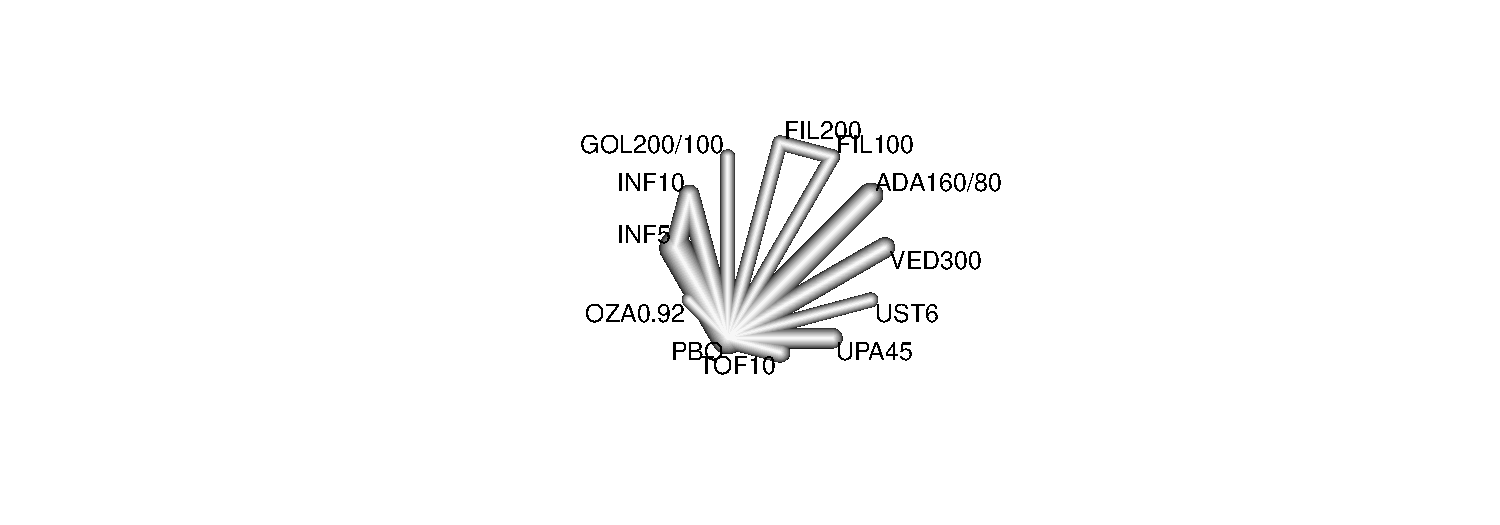
\includegraphics{chapter_10_files/figure-pdf/unnamed-chunk-27-1.pdf}

}

\caption{Evidence network of 18 trials that contributed efficacy data
for induction in bio-naive populations}

\end{figure}

Below, we conduct a random effects network meta-analysis of the reported
study effects (expressed as odds ratio) and consider placebo
(\texttt{treat\ =\ "PBO"}) as the control treatment.

\begin{Shaded}
\begin{Highlighting}[]
\NormalTok{NMA.uc }\OtherTok{\textless{}{-}} \FunctionTok{netmeta}\NormalTok{(}\AttributeTok{TE =}\NormalTok{ TE, }\AttributeTok{seTE =}\NormalTok{ seTE, }\AttributeTok{treat1 =}\NormalTok{ treat1, }\AttributeTok{treat2 =}\NormalTok{ treat2,}
                  \AttributeTok{studlab =}\NormalTok{ studlab, }\AttributeTok{data =}\NormalTok{ UlcerativeColitis, }\AttributeTok{sm =} \StringTok{"OR"}\NormalTok{, }
                  \AttributeTok{ref =} \StringTok{"PBO"}\NormalTok{, }\AttributeTok{common =} \ConstantTok{FALSE}\NormalTok{, }\AttributeTok{comb.random =} \ConstantTok{TRUE}\NormalTok{)}
\NormalTok{NMA.uc}
\end{Highlighting}
\end{Shaded}

All treatments except \texttt{FIL100} and \texttt{UST6} are
significantly more efficacious than \texttt{PBO} at inducing clinical
remission. We can now estimate the probabilities of each treatment being
at each possible rank and the SUCRAs (Surface Under the Cumulative
RAnking curve):

\begin{Shaded}
\begin{Highlighting}[]
\NormalTok{sucra.uc }\OtherTok{\textless{}{-}} \FunctionTok{rankogram}\NormalTok{(NMA.uc, }\AttributeTok{nsim =} \DecValTok{100}\NormalTok{, }\AttributeTok{random =} \ConstantTok{TRUE}\NormalTok{, }\AttributeTok{common =} \ConstantTok{FALSE}\NormalTok{, }
                      \AttributeTok{small.values =} \StringTok{"undesirable"}\NormalTok{)}

\CommentTok{\# Exctract the SUCRA values}
\NormalTok{sucra.uc}\SpecialCharTok{$}\NormalTok{ranking.random}
\end{Highlighting}
\end{Shaded}

\begin{verbatim}
 ADA160/80     FIL100     FIL200 GOL200/100      INF10       INF5    OZA0.92 
0.26000000 0.17363636 0.44818182 0.65363636 0.59181818 0.76454545 0.74909091 
       PBO      TOF10      UPA45       UST6     VED300 
0.01363636 0.40545455 0.97272727 0.34909091 0.61818182 
\end{verbatim}

These results indicate that 97.3\% of the evaluated treatments are worse
than \texttt{UPA45}.

\hypertarget{version-info-4}{%
\section*{Version info}\label{version-info-4}}
\addcontentsline{toc}{section}{Version info}

\markright{Version info}

This chapter was rendered using the following version of R and its
packages:

\begin{verbatim}
R version 4.2.3 (2023-03-15 ucrt)
Platform: x86_64-w64-mingw32/x64 (64-bit)
Running under: Windows 10 x64 (build 19045)

Matrix products: default

locale:
[1] LC_COLLATE=Dutch_Netherlands.utf8  LC_CTYPE=Dutch_Netherlands.utf8   
[3] LC_MONETARY=Dutch_Netherlands.utf8 LC_NUMERIC=C                      
[5] LC_TIME=Dutch_Netherlands.utf8    

attached base packages:
[1] stats     graphics  grDevices utils     datasets  methods   base     

other attached packages:
[1] dmetar_0.0.9000  netmeta_2.8-2    meta_6.5-0       gemtc_1.0-1     
[5] coda_0.19-4      dplyr_1.1.2      kableExtra_1.3.4

loaded via a namespace (and not attached):
 [1] httr_1.4.6          magic_1.6-1         jsonlite_1.8.5     
 [4] viridisLite_0.4.2   splines_4.2.3       stats4_4.2.3       
 [7] metafor_4.2-0       slam_0.1-50         yaml_2.3.7         
[10] robustbase_0.99-0   ggrepel_0.9.3       numDeriv_2016.8-1.1
[13] pillar_1.9.0        lattice_0.21-8      glue_1.6.2         
[16] digest_0.6.31       rvest_1.0.3         minqa_1.2.5        
[19] colorspace_2.1-0    MuMIn_1.47.5        htmltools_0.5.5    
[22] Matrix_1.5-4.1      plyr_1.8.8          pkgconfig_2.0.3    
[25] mvtnorm_1.2-2       Rglpk_0.6-5         scales_1.2.1       
[28] webshot_0.5.4       svglite_2.1.1       rjags_4-14         
[31] metadat_1.2-0       lme4_1.1-33         tibble_3.2.1       
[34] farver_2.1.1        generics_0.1.3      ggplot2_3.4.2      
[37] withr_2.5.0         nnet_7.3-19         cli_3.6.1          
[40] magrittr_2.0.3      mclust_6.0.0        evaluate_0.21      
[43] fansi_1.0.4         nlme_3.1-162        MASS_7.3-60        
[46] truncnorm_1.0-9     forcats_1.0.0       xml2_1.3.4         
[49] class_7.3-22        tools_4.2.3         lifecycle_1.0.3    
[52] stringr_1.5.0       kernlab_0.9-32      munsell_0.5.0      
[55] cluster_2.1.4       fpc_2.2-10          compiler_4.2.3     
[58] systemfonts_1.0.4   rlang_1.1.1         grid_4.2.3         
[61] nloptr_2.0.3        rstudioapi_0.14     CompQuadForm_1.4.3 
[64] igraph_1.5.0        labeling_0.4.2      rmarkdown_2.22     
[67] boot_1.3-28.1       gtable_0.3.3        codetools_0.2-19   
[70] abind_1.4-5         flexmix_2.3-19      R6_2.5.1           
[73] gridExtra_2.3       knitr_1.43          prabclus_2.3-2     
[76] fastmap_1.1.1       utf8_1.2.3          mathjaxr_1.6-0     
[79] poibin_1.5          modeltools_0.2-23   stringi_1.7.12     
[82] parallel_4.2.3      Rcpp_1.0.10         vctrs_0.6.3        
[85] DEoptimR_1.0-14     tidyselect_1.2.0    xfun_0.39          
[88] diptest_0.76-0     
\end{verbatim}

\hypertarget{references-1}{%
\section*{References}\label{references-1}}
\addcontentsline{toc}{section}{References}

\markright{References}

\bookmarksetup{startatroot}

\hypertarget{dealing-with-irregular-and-informative-visits}{%
\chapter{Dealing with irregular and informative
visits}\label{dealing-with-irregular-and-informative-visits}}

Janie Coulombe (Université de Montréal)\\
Thomas Debray (Smart Data Analysis and Statistics B.V.)

\hfill\break

\hypertarget{introduction-2}{%
\section{Introduction}\label{introduction-2}}

We first load the required packages

\begin{Shaded}
\begin{Highlighting}[]
\FunctionTok{library}\NormalTok{(dplyr)}
\FunctionTok{library}\NormalTok{(broom)}
\FunctionTok{library}\NormalTok{(ggplot2)}
\FunctionTok{library}\NormalTok{(mice)}
\end{Highlighting}
\end{Shaded}

Subsequently, we load the relevant R scripts:

\begin{Shaded}
\begin{Highlighting}[]
\FunctionTok{source}\NormalTok{(}\StringTok{"resources/chapter12\_sim.r"}\NormalTok{)}
\end{Highlighting}
\end{Shaded}

\begin{verbatim}
Loading required package: nlme
\end{verbatim}

\begin{verbatim}

Attaching package: 'nlme'
\end{verbatim}

\begin{verbatim}
The following object is masked from 'package:dplyr':

    collapse
\end{verbatim}

\begin{verbatim}
Loading required package: MASS
\end{verbatim}

\begin{verbatim}

Attaching package: 'MASS'
\end{verbatim}

\begin{verbatim}
The following object is masked from 'package:dplyr':

    select
\end{verbatim}

\begin{verbatim}
Loading required package: truncnorm
\end{verbatim}

\begin{Shaded}
\begin{Highlighting}[]
\FunctionTok{source}\NormalTok{(}\StringTok{"resources/chapter12\_fig\_functions.r"}\NormalTok{)}
\FunctionTok{source}\NormalTok{(}\StringTok{"resources/chapter12\_mlmi.r"}\NormalTok{)}
\end{Highlighting}
\end{Shaded}

\hypertarget{example-dataset}{%
\section{Example dataset}\label{example-dataset}}

Below, we generate an example dataset that contains information on the
treatment allocation \texttt{x} and three baseline covariates
\texttt{age}, \texttt{sex} and \texttt{edss} (EDSS at treatment start).
The discrete outcome \texttt{y} represents the Expanded Disability
Status Scale (EDSS) score after \texttt{time} months of treatment
exposure. Briefly, the EDSS is a semi-continuous measure that varies
from 0 (no disability) to 10 (death).

\begin{Shaded}
\begin{Highlighting}[]
\FunctionTok{set.seed}\NormalTok{(}\DecValTok{9843626}\NormalTok{)}

\NormalTok{dataset  }\OtherTok{\textless{}{-}} \FunctionTok{sim\_data\_EDSS}\NormalTok{(}\AttributeTok{npatients =} \DecValTok{500}\NormalTok{,}
                          \AttributeTok{ncenters =} \DecValTok{10}\NormalTok{,}
                          \AttributeTok{follow\_up =} \DecValTok{12}\SpecialCharTok{*}\DecValTok{5}\NormalTok{, }\CommentTok{\# Total follow{-}up (number of months)}
                          \AttributeTok{sd\_a\_t =} \FloatTok{0.5}\NormalTok{,   }\CommentTok{\# DGM {-} Within{-}visit variation in EDSS scores}
                          \AttributeTok{baseline\_EDSS =} \FloatTok{1.3295}\NormalTok{,    }\CommentTok{\# DGM {-} Mean baseline EDDS score}
                          \AttributeTok{sd\_alpha\_ij =} \FloatTok{1.46}\NormalTok{,    }\CommentTok{\# DGM {-} Between{-}subject variation in baseline EDSS}
                          \AttributeTok{sd\_beta1\_j =} \FloatTok{0.20}\NormalTok{,    }\CommentTok{\# DGM {-} Between{-}site variation in baseline EDSS}
                          \AttributeTok{mean\_age =} \FloatTok{42.41}\NormalTok{,}
                          \AttributeTok{sd\_age =} \FloatTok{10.53}\NormalTok{,}
                          \AttributeTok{min\_age =} \DecValTok{18}\NormalTok{,}
                          \AttributeTok{beta\_age =} \FloatTok{0.05}\NormalTok{, }\CommentTok{\# DGM {-} prognostic effect of age}
                          \AttributeTok{beta\_t =} \FloatTok{0.014}\NormalTok{,  }\CommentTok{\# DGM {-} prognostic effect of time}
                          \AttributeTok{beta\_t2 =} \DecValTok{0}\NormalTok{,    }\CommentTok{\# DGM {-} prognostic effect of time squared}
                          \AttributeTok{delta\_xt =} \DecValTok{0}\NormalTok{, }\CommentTok{\# DGM {-} interaction treatment time}
                          \AttributeTok{delta\_xt2 =} \DecValTok{0}\NormalTok{, }\CommentTok{\# 0.0005    \# DGM {-} interaction treatment time2}
                          \AttributeTok{p\_female =} \FloatTok{0.75}\NormalTok{, }
                          \AttributeTok{beta\_female =} \SpecialCharTok{{-}}\FloatTok{0.2}\NormalTok{ ,  }\DocumentationTok{\#\# DGM {-} prognostic effect of male sex}
                          \AttributeTok{delta\_xf =} \DecValTok{0}\NormalTok{,      }\DocumentationTok{\#\# DGM {-} interaction sex treatment       }
                          \AttributeTok{rho =} \FloatTok{0.8}\NormalTok{,             }\CommentTok{\# DGM {-} autocorrelation of between alpha\_tij}
                          \AttributeTok{corFUN =}\NormalTok{ corAR1,       }\CommentTok{\# DGM {-} correlation structure of the latent EDSS scores}
                          \AttributeTok{tx\_alloc\_FUN =}\NormalTok{ treatment\_alloc\_confounding\_v2 ) }\DocumentationTok{\#\# or treatment\_alloc\_randomized}
\end{Highlighting}
\end{Shaded}

\begin{figure}

{\centering 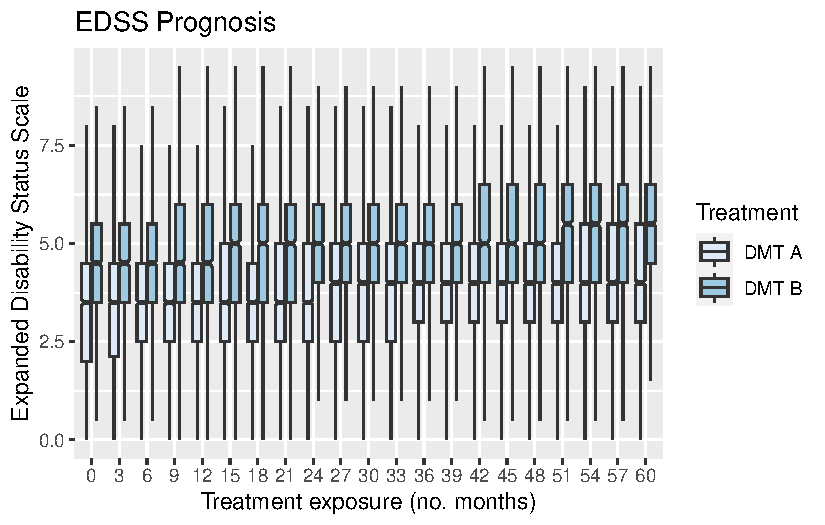
\includegraphics{chapter_12_files/figure-pdf/unnamed-chunk-4-1.pdf}

}

\caption{Distribution of the EDSS score at each time point}

\end{figure}

We remove the outcome \texttt{y} according to the informative visit
process that depends on the received treatment, gender, and age.

\begin{Shaded}
\begin{Highlighting}[]
\NormalTok{dataset\_visit }\OtherTok{\textless{}{-}} \FunctionTok{censor\_visits\_a5}\NormalTok{(dataset, }\AttributeTok{seed =} \DecValTok{12345}\NormalTok{) }\SpecialCharTok{\%\textgreater{}\%} 
\NormalTok{  dplyr}\SpecialCharTok{::}\FunctionTok{select}\NormalTok{(}\SpecialCharTok{{-}}\NormalTok{y) }\SpecialCharTok{\%\textgreater{}\%}
  \FunctionTok{mutate}\NormalTok{(}\AttributeTok{time\_x =}\NormalTok{ time}\SpecialCharTok{*}\NormalTok{x)}
\end{Highlighting}
\end{Shaded}

In the censored data, a total of 17 out of 5000 patients have a visit at
\texttt{time=60}.

\hypertarget{estimation-of-treatment-effect}{%
\section{Estimation of treatment
effect}\label{estimation-of-treatment-effect}}

We will estimate the marginal treatment effect at time \texttt{time=60}.

\hypertarget{original-data}{%
\subsection{Original data}\label{original-data}}

\begin{Shaded}
\begin{Highlighting}[]
\NormalTok{origdat60 }\OtherTok{\textless{}{-}}\NormalTok{ dataset }\SpecialCharTok{\%\textgreater{}\%} \FunctionTok{filter}\NormalTok{(time }\SpecialCharTok{==} \DecValTok{60}\NormalTok{)}

\CommentTok{\# Predict probability of treatment allocation}
\NormalTok{fitps }\OtherTok{\textless{}{-}} \FunctionTok{glm}\NormalTok{(x }\SpecialCharTok{\textasciitilde{}}\NormalTok{ age }\SpecialCharTok{+}\NormalTok{ sex }\SpecialCharTok{+}\NormalTok{ edss, }\AttributeTok{family =} \StringTok{\textquotesingle{}binomial\textquotesingle{}}\NormalTok{, }
             \AttributeTok{data =}\NormalTok{ origdat60)}

\CommentTok{\# Derive the propensity score}
\NormalTok{origdat60 }\OtherTok{\textless{}{-}}\NormalTok{ origdat60 }\SpecialCharTok{\%\textgreater{}\%} \FunctionTok{mutate}\NormalTok{(}\AttributeTok{ipt =} \FunctionTok{ifelse}\NormalTok{(x }\SpecialCharTok{==} \DecValTok{1}\NormalTok{, }\DecValTok{1}\SpecialCharTok{/}\FunctionTok{predict}\NormalTok{(fitps, }\AttributeTok{type =} \StringTok{\textquotesingle{}response\textquotesingle{}}\NormalTok{),}
                                               \DecValTok{1}\SpecialCharTok{/}\NormalTok{(}\DecValTok{1}\SpecialCharTok{{-}}\FunctionTok{predict}\NormalTok{(fitps, }\AttributeTok{type =} \StringTok{\textquotesingle{}response\textquotesingle{}}\NormalTok{))))}

\CommentTok{\# Estimate }
\NormalTok{fit\_ref\_m }\OtherTok{\textless{}{-}} \FunctionTok{tidy}\NormalTok{(}\FunctionTok{lm}\NormalTok{(y }\SpecialCharTok{\textasciitilde{}}\NormalTok{ x, }\AttributeTok{weight =}\NormalTok{ ipt, }\AttributeTok{data =}\NormalTok{ origdat60), }\AttributeTok{conf.int =} \ConstantTok{TRUE}\NormalTok{) }
\end{Highlighting}
\end{Shaded}

\hypertarget{doubly-weighted-marginal-treatment-effect}{%
\subsection{Doubly-weighted marginal treatment
effect}\label{doubly-weighted-marginal-treatment-effect}}

We here implement inverse probability of response weights into the
estimating equations to adjust for nonrandom missingness Coulombe,
Moodie, and Platt (2020).

\begin{Shaded}
\begin{Highlighting}[]
\NormalTok{obsdat60 }\OtherTok{\textless{}{-}}\NormalTok{ dataset\_visit }\SpecialCharTok{\%\textgreater{}\%} \FunctionTok{mutate}\NormalTok{(}\AttributeTok{visit =} \FunctionTok{ifelse}\NormalTok{(}\FunctionTok{is.na}\NormalTok{(y\_obs),}\DecValTok{0}\NormalTok{,}\DecValTok{1}\NormalTok{)) }\SpecialCharTok{\%\textgreater{}\%} \FunctionTok{filter}\NormalTok{(time }\SpecialCharTok{==} \DecValTok{60}\NormalTok{)}

\NormalTok{gamma }\OtherTok{\textless{}{-}} \FunctionTok{glm}\NormalTok{(visit }\SpecialCharTok{\textasciitilde{}}\NormalTok{ x }\SpecialCharTok{+}\NormalTok{ sex }\SpecialCharTok{+}\NormalTok{ age }\SpecialCharTok{+}\NormalTok{ edss, }\AttributeTok{family =} \StringTok{\textquotesingle{}binomial\textquotesingle{}}\NormalTok{, }\AttributeTok{data =}\NormalTok{ obsdat60)}\SpecialCharTok{$}\NormalTok{coef   }

\NormalTok{obsdat60 }\OtherTok{\textless{}{-}}\NormalTok{ obsdat60 }\SpecialCharTok{\%\textgreater{}\%} \FunctionTok{mutate}\NormalTok{(}\AttributeTok{rho\_i =} \DecValTok{1}\SpecialCharTok{/}\FunctionTok{exp}\NormalTok{(gamma[}\StringTok{"(Intercept)"}\NormalTok{] }\SpecialCharTok{+}
\NormalTok{                                                          gamma[}\StringTok{"x"}\NormalTok{]}\SpecialCharTok{*}\NormalTok{x }\SpecialCharTok{+}
\NormalTok{                                                          gamma[}\StringTok{"sex"}\NormalTok{]}\SpecialCharTok{*}\NormalTok{sex }\SpecialCharTok{+}
\NormalTok{                                                          gamma[}\StringTok{"age"}\NormalTok{]}\SpecialCharTok{*}\NormalTok{age))}

\CommentTok{\# Predict probability of treatment allocation}
\NormalTok{fitps }\OtherTok{\textless{}{-}} \FunctionTok{glm}\NormalTok{(x }\SpecialCharTok{\textasciitilde{}}\NormalTok{ age }\SpecialCharTok{+}\NormalTok{ sex }\SpecialCharTok{+}\NormalTok{ edss, }\AttributeTok{family=}\StringTok{\textquotesingle{}binomial\textquotesingle{}}\NormalTok{, }\AttributeTok{data =}\NormalTok{ obsdat60)}

\CommentTok{\# Derive the propensity score}
\NormalTok{obsdat60 }\OtherTok{\textless{}{-}}\NormalTok{ obsdat60 }\SpecialCharTok{\%\textgreater{}\%} \FunctionTok{mutate}\NormalTok{(}\AttributeTok{ipt =} \FunctionTok{ifelse}\NormalTok{(x}\SpecialCharTok{==}\DecValTok{1}\NormalTok{, }\DecValTok{1}\SpecialCharTok{/}\FunctionTok{predict}\NormalTok{(fitps, }\AttributeTok{type=}\StringTok{\textquotesingle{}response\textquotesingle{}}\NormalTok{),}
                                            \DecValTok{1}\SpecialCharTok{/}\NormalTok{(}\DecValTok{1}\SpecialCharTok{{-}}\FunctionTok{predict}\NormalTok{(fitps, }\AttributeTok{type=}\StringTok{\textquotesingle{}response\textquotesingle{}}\NormalTok{))))}


\NormalTok{fit\_w }\OtherTok{\textless{}{-}} \FunctionTok{tidy}\NormalTok{(}\FunctionTok{lm}\NormalTok{(y\_obs }\SpecialCharTok{\textasciitilde{}}\NormalTok{ x, }\AttributeTok{weights =}\NormalTok{ ipt}\SpecialCharTok{*}\NormalTok{rho\_i, }\AttributeTok{data =}\NormalTok{ obsdat60), }\AttributeTok{conf.int =} \ConstantTok{TRUE}\NormalTok{)}
\end{Highlighting}
\end{Shaded}

\hypertarget{multilevel-multiple-imputation}{%
\subsection{Multilevel multiple
imputation}\label{multilevel-multiple-imputation}}

We adopt the imputation approach proposed by Debray et al. (2023).
Briefly, we impute the entire vector of \texttt{y\_obs} for all 61
potential visits and generate 10 imputed datasets. Note: \texttt{mlmi}
currently does not support imputation of treatment-covariate interaction
terms.

\begin{Shaded}
\begin{Highlighting}[]
\NormalTok{imp }\OtherTok{\textless{}{-}} \FunctionTok{impute\_y\_mice\_3l}\NormalTok{(dataset\_visit, }\AttributeTok{seed =} \DecValTok{12345}\NormalTok{)}
\end{Highlighting}
\end{Shaded}

We can now estimate the treatment effect in each imputed dataset

\begin{Shaded}
\begin{Highlighting}[]
\CommentTok{\# Predict probability of treatment allocation}
\NormalTok{fitps }\OtherTok{\textless{}{-}} \FunctionTok{glm}\NormalTok{(x }\SpecialCharTok{\textasciitilde{}}\NormalTok{ age }\SpecialCharTok{+}\NormalTok{ sex }\SpecialCharTok{+}\NormalTok{ edss, }\AttributeTok{family=}\StringTok{\textquotesingle{}binomial\textquotesingle{}}\NormalTok{, }\AttributeTok{data =}\NormalTok{ dataset\_visit)}
  
\CommentTok{\# Derive the propensity score}
\NormalTok{dataset\_visit }\OtherTok{\textless{}{-}}\NormalTok{ dataset\_visit }\SpecialCharTok{\%\textgreater{}\%} \FunctionTok{mutate}\NormalTok{(}\AttributeTok{ipt =} \FunctionTok{ifelse}\NormalTok{(x}\SpecialCharTok{==}\DecValTok{1}\NormalTok{, }\DecValTok{1}\SpecialCharTok{/}\FunctionTok{predict}\NormalTok{(fitps, }\AttributeTok{type=}\StringTok{\textquotesingle{}response\textquotesingle{}}\NormalTok{),}
                                                       \DecValTok{1}\SpecialCharTok{/}\NormalTok{(}\DecValTok{1}\SpecialCharTok{{-}}\FunctionTok{predict}\NormalTok{(fitps, }\AttributeTok{type=}\StringTok{\textquotesingle{}response\textquotesingle{}}\NormalTok{))))}
  
\NormalTok{Q }\OtherTok{\textless{}{-}}\NormalTok{ U }\OtherTok{\textless{}{-}} \FunctionTok{rep}\NormalTok{(}\ConstantTok{NA}\NormalTok{, }\DecValTok{10}\NormalTok{) }\CommentTok{\# Error variances}

\ControlFlowTok{for}\NormalTok{ (i }\ControlFlowTok{in} \FunctionTok{seq}\NormalTok{(}\DecValTok{10}\NormalTok{)) \{}
\NormalTok{  dati }\OtherTok{\textless{}{-}} \FunctionTok{cbind}\NormalTok{(dataset\_visit[,}\FunctionTok{c}\NormalTok{(}\StringTok{"x"}\NormalTok{,}\StringTok{"ipt"}\NormalTok{,}\StringTok{"time"}\NormalTok{)], }\AttributeTok{y\_imp =}\NormalTok{ imp[,i]) }\SpecialCharTok{\%\textgreater{}\%} \FunctionTok{filter}\NormalTok{(time }\SpecialCharTok{==} \DecValTok{60}\NormalTok{)}
  
  \CommentTok{\# Estimate }
\NormalTok{  fit }\OtherTok{\textless{}{-}} \FunctionTok{tidy}\NormalTok{(}\FunctionTok{lm}\NormalTok{(y\_imp }\SpecialCharTok{\textasciitilde{}}\NormalTok{ x, }\AttributeTok{weight =}\NormalTok{ ipt, }\AttributeTok{data =}\NormalTok{ dati), }\AttributeTok{conf.int =} \ConstantTok{TRUE}\NormalTok{) }
  
\NormalTok{  Q[i] }\OtherTok{\textless{}{-}}\NormalTok{ fit }\SpecialCharTok{\%\textgreater{}\%} \FunctionTok{filter}\NormalTok{(term }\SpecialCharTok{==} \StringTok{"x"}\NormalTok{) }\SpecialCharTok{\%\textgreater{}\%} \FunctionTok{pull}\NormalTok{(estimate)}
\NormalTok{  U[i] }\OtherTok{\textless{}{-}}\NormalTok{ (fit }\SpecialCharTok{\%\textgreater{}\%} \FunctionTok{filter}\NormalTok{(term }\SpecialCharTok{==} \StringTok{"x"}\NormalTok{) }\SpecialCharTok{\%\textgreater{}\%} \FunctionTok{pull}\NormalTok{(std.error))}\SpecialCharTok{**}\DecValTok{2}
\NormalTok{\}}

\NormalTok{fit\_mlmi }\OtherTok{\textless{}{-}} \FunctionTok{pool.scalar}\NormalTok{(}\AttributeTok{Q =}\NormalTok{ Q, }\AttributeTok{U =}\NormalTok{ U)}
\end{Highlighting}
\end{Shaded}

\hypertarget{reproduce-the-results-using-all-data-to-compute-the-marginal-effect-with-iiv-weighted}{%
\section{Reproduce the results using all data to compute the marginal
effect with
IIV-weighted}\label{reproduce-the-results-using-all-data-to-compute-the-marginal-effect-with-iiv-weighted}}

\hypertarget{doubly--weighted-marginal-treatment-effect-total}{%
\subsection{Doubly -weighted marginal treatment effect
total}\label{doubly--weighted-marginal-treatment-effect-total}}

\begin{Shaded}
\begin{Highlighting}[]
\NormalTok{obsdatall }\OtherTok{\textless{}{-}}\NormalTok{ dataset\_visit }\SpecialCharTok{\%\textgreater{}\%} \FunctionTok{mutate}\NormalTok{(}\AttributeTok{visit =} \FunctionTok{ifelse}\NormalTok{(}\FunctionTok{is.na}\NormalTok{(y\_obs),}\DecValTok{0}\NormalTok{,}\DecValTok{1}\NormalTok{))  }
\NormalTok{gamma }\OtherTok{\textless{}{-}} \FunctionTok{glm}\NormalTok{(visit }\SpecialCharTok{\textasciitilde{}}\NormalTok{ x }\SpecialCharTok{+}\NormalTok{ sex }\SpecialCharTok{+}\NormalTok{ age }\SpecialCharTok{+}\NormalTok{ edss, }\AttributeTok{family =} \StringTok{\textquotesingle{}binomial\textquotesingle{}}\NormalTok{, }\AttributeTok{data =}\NormalTok{ obsdatall)}\SpecialCharTok{$}\NormalTok{coef   }
\NormalTok{obsdatall }\OtherTok{\textless{}{-}}\NormalTok{ obsdatall }\SpecialCharTok{\%\textgreater{}\%} \FunctionTok{mutate}\NormalTok{(}\AttributeTok{rho\_i =} \DecValTok{1}\SpecialCharTok{/}\FunctionTok{exp}\NormalTok{(gamma[}\StringTok{"(Intercept)"}\NormalTok{] }\SpecialCharTok{+}
\NormalTok{                                                gamma[}\StringTok{"x"}\NormalTok{]}\SpecialCharTok{*}\NormalTok{x }\SpecialCharTok{+}
\NormalTok{                                                gamma[}\StringTok{"sex"}\NormalTok{]}\SpecialCharTok{*}\NormalTok{sex }\SpecialCharTok{+}
\NormalTok{                                                gamma[}\StringTok{"age"}\NormalTok{]}\SpecialCharTok{*}\NormalTok{age))}
\CommentTok{\# Predict probability of treatment allocation}
\NormalTok{fitps }\OtherTok{\textless{}{-}} \FunctionTok{glm}\NormalTok{(x }\SpecialCharTok{\textasciitilde{}}\NormalTok{ age }\SpecialCharTok{+}\NormalTok{ sex }\SpecialCharTok{+}\NormalTok{ edss, }\AttributeTok{family=}\StringTok{\textquotesingle{}binomial\textquotesingle{}}\NormalTok{, }\AttributeTok{data =}\NormalTok{ obsdatall)}
\CommentTok{\# Derive the propensity score}
\NormalTok{obsdatall }\OtherTok{\textless{}{-}}\NormalTok{ obsdatall }\SpecialCharTok{\%\textgreater{}\%} \FunctionTok{mutate}\NormalTok{(}\AttributeTok{ipt =} \FunctionTok{ifelse}\NormalTok{(x}\SpecialCharTok{==}\DecValTok{1}\NormalTok{, }\DecValTok{1}\SpecialCharTok{/}\FunctionTok{predict}\NormalTok{(fitps, }\AttributeTok{type=}\StringTok{\textquotesingle{}response\textquotesingle{}}\NormalTok{),}
                                             \DecValTok{1}\SpecialCharTok{/}\NormalTok{(}\DecValTok{1}\SpecialCharTok{{-}}\FunctionTok{predict}\NormalTok{(fitps, }\AttributeTok{type=}\StringTok{\textquotesingle{}response\textquotesingle{}}\NormalTok{))))}
\NormalTok{fit\_w }\OtherTok{\textless{}{-}} \FunctionTok{tidy}\NormalTok{(}\FunctionTok{lm}\NormalTok{(y\_obs }\SpecialCharTok{\textasciitilde{}}\NormalTok{ x, }\AttributeTok{weights =}\NormalTok{ ipt}\SpecialCharTok{*}\NormalTok{rho\_i, }\AttributeTok{data =}\NormalTok{ obsdatall), }\AttributeTok{conf.int =} \ConstantTok{TRUE}\NormalTok{)}
\end{Highlighting}
\end{Shaded}

\hypertarget{results}{%
\section{Results}\label{results}}

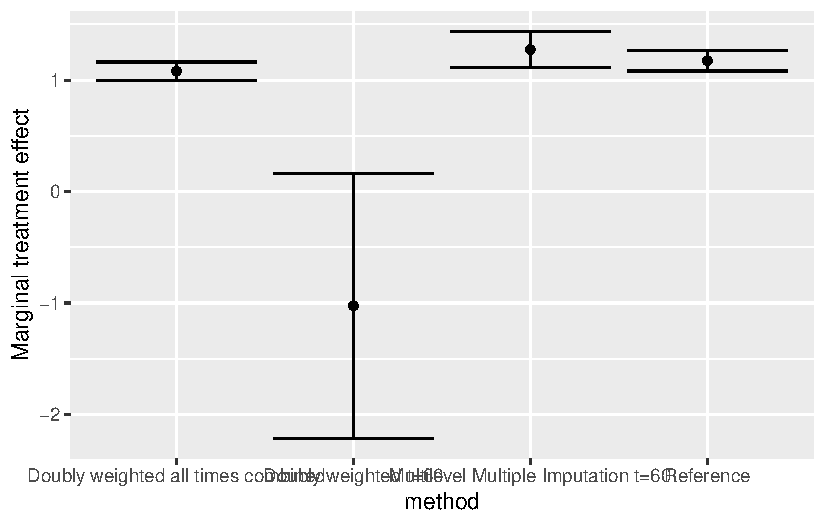
\includegraphics{chapter_12_files/figure-pdf/unnamed-chunk-17-1.pdf}

\hypertarget{version-info-5}{%
\section*{Version info}\label{version-info-5}}
\addcontentsline{toc}{section}{Version info}

\markright{Version info}

This chapter was rendered using the following version of R and its
packages:

\begin{verbatim}
R version 4.2.3 (2023-03-15 ucrt)
Platform: x86_64-w64-mingw32/x64 (64-bit)
Running under: Windows 10 x64 (build 19045)

Matrix products: default

locale:
[1] LC_COLLATE=Dutch_Netherlands.utf8  LC_CTYPE=Dutch_Netherlands.utf8   
[3] LC_MONETARY=Dutch_Netherlands.utf8 LC_NUMERIC=C                      
[5] LC_TIME=Dutch_Netherlands.utf8    

attached base packages:
[1] stats     graphics  grDevices utils     datasets  methods   base     

other attached packages:
[1] truncnorm_1.0-9 MASS_7.3-60     nlme_3.1-162    mice_3.16.0    
[5] ggplot2_3.4.2   broom_1.0.5     dplyr_1.1.2    

loaded via a namespace (and not attached):
 [1] shape_1.4.6        tidyselect_1.2.0   xfun_0.39          purrr_1.0.1       
 [5] splines_4.2.3      lattice_0.21-8     colorspace_2.1-0   vctrs_0.6.3       
 [9] generics_0.1.3     htmltools_0.5.5    yaml_2.3.7         pan_1.6           
[13] utf8_1.2.3         survival_3.5-5     rlang_1.1.1        jomo_2.7-6        
[17] pillar_1.9.0       nloptr_2.0.3       glue_1.6.2         withr_2.5.0       
[21] RColorBrewer_1.1-3 foreach_1.5.2      lifecycle_1.0.3    munsell_0.5.0     
[25] gtable_0.3.3       codetools_0.2-19   evaluate_0.21      labeling_0.4.2    
[29] knitr_1.43         fastmap_1.1.1      fansi_1.0.4        Rcpp_1.0.10       
[33] scales_1.2.1       backports_1.4.1    jsonlite_1.8.5     farver_2.1.1      
[37] lme4_1.1-33        digest_0.6.31      grid_4.2.3         cli_3.6.1         
[41] tools_4.2.3        magrittr_2.0.3     glmnet_4.1-7       tibble_3.2.1      
[45] tidyr_1.3.0        pkgconfig_2.0.3    ellipsis_0.3.2     Matrix_1.5-4.1    
[49] minqa_1.2.5        rmarkdown_2.22     rstudioapi_0.14    iterators_1.0.14  
[53] rpart_4.1.19       mitml_0.4-5        R6_2.5.1           boot_1.3-28.1     
[57] nnet_7.3-19        compiler_4.2.3    
\end{verbatim}

\hypertarget{references-2}{%
\section*{References}\label{references-2}}
\addcontentsline{toc}{section}{References}

\markright{References}

\bookmarksetup{startatroot}

\hypertarget{prediction-of-individual-treatment-effect-using-data-from-multiple-studies}{%
\chapter{Prediction of individual treatment effect using data from
multiple
studies}\label{prediction-of-individual-treatment-effect-using-data-from-multiple-studies}}

Orestis Efthimiou (Institute of Social and Preventive Medicine (ISPM))

\hfill\break

In this chapter, we discuss statistical methods for developing models to
predict patient-level treatment effects using data from multiple
randomized and non-randomized studies. We will first present prediction
models that assume a constant treatment effect and discuss how to
address heterogeneity in baseline risk. Subsequently, we will discuss
approaches that allow for treatment effect modification by adopting two
different approaches in an IPD-MA context, namely the risk modelling and
the effect modelling approach. For both approaches, we will first
discuss how to combine IPD from RCTs comparing the same two treatments.
We will then discuss how these methods can be extended to include
randomized data from multiple treatments, real-world data, and published
aggregate data. We will discuss statistical software to implement these
approaches and provide example code as supporting information. Real
examples will be used throughout to illustrate the main methods.

\hypertarget{estimating-heterogeneous-treatment-effects-in-pairwise-meta-analysis}{%
\section{Estimating heterogeneous treatment effects in pairwise
meta-analysis}\label{estimating-heterogeneous-treatment-effects-in-pairwise-meta-analysis}}

We hereby provide code for estimating patient-level treatment effects
for the case when we have patient-level data from multiple randomized
trials.

\hypertarget{example-of-a-continuous-outcome}{%
\subsection{Example of a continuous
outcome}\label{example-of-a-continuous-outcome}}

\hypertarget{setup}{%
\subsubsection{Setup}\label{setup}}

We start by simulating an artificial dataset using the R package
\textbf{bipd}:

\begin{Shaded}
\begin{Highlighting}[]
\FunctionTok{library}\NormalTok{(bipd)}
\NormalTok{ds }\OtherTok{\textless{}{-}} \FunctionTok{generate\_ipdma\_example}\NormalTok{(}\AttributeTok{type =} \StringTok{"continuous"}\NormalTok{)}
\end{Highlighting}
\end{Shaded}

Let us have a look at the dataset:

\begin{Shaded}
\begin{Highlighting}[]
\FunctionTok{head}\NormalTok{(ds)}
\end{Highlighting}
\end{Shaded}

\begin{verbatim}
  studyid treat         z1         z2  y
1       1     0  0.3266390 -1.7236365 11
2       1     0  0.4951180 -2.2374921 11
3       1     0 -0.7056270 -1.3584076 11
4       1     1 -0.9785132 -0.3029899  8
5       1     0  0.2651324 -0.1735689 11
6       1     1  1.3853282 -0.2320760  6
\end{verbatim}

The simulated dataset contains information on the following variables:

\begin{itemize}
\tightlist
\item
  the trial indicator \texttt{studyid}
\item
  the treatment indicator \texttt{treat}, which takes the values 0 for
  control and 1 for active treatment
\item
  two prognostic variables \texttt{z1} and \texttt{z2}
\item
  the continuous outcome \texttt{y}
\end{itemize}

\hypertarget{tbl-summary-continuous_outcome-data}{}
\begin{table}
\caption{\label{tbl-summary-continuous_outcome-data}The simulated dataset with a continuous outcome }\tabularnewline

\centering
\begin{tabular}[t]{llll}
\toprule
  & 0 & 1 & Overall\\
\midrule
 & (N=321) & (N=279) & (N=600)\\
\addlinespace[0.3em]
\multicolumn{4}{l}{\textbf{z1}}\\
\hspace{1em}Mean (SD) & 0.0681 (0.967) & 0.0166 (0.983) & 0.0441 (0.974)\\
\hspace{1em}Median [Min, Max] & 0.0464 [-3.13, 2.87] & -0.0316 [-2.69, 2.50] & 0.0244 [-3.13, 2.87]\\
\addlinespace[0.3em]
\multicolumn{4}{l}{\textbf{z2}}\\
\hspace{1em}Mean (SD) & -0.0961 (0.990) & 0.0117 (1.01) & -0.0459 (1.00)\\
\hspace{1em}Median [Min, Max] & -0.117 [-2.55, 2.52] & 0.0838 [-3.54, 3.38] & -0.0371 [-3.54, 3.38]\\
\addlinespace[0.3em]
\multicolumn{4}{l}{\textbf{studyid}}\\
\hspace{1em}1 & 57 (17.8\%) & 43 (15.4\%) & 100 (16.7\%)\\
\hspace{1em}2 & 61 (19.0\%) & 39 (14.0\%) & 100 (16.7\%)\\
\hspace{1em}3 & 50 (15.6\%) & 50 (17.9\%) & 100 (16.7\%)\\
\hspace{1em}4 & 51 (15.9\%) & 49 (17.6\%) & 100 (16.7\%)\\
\hspace{1em}5 & 57 (17.8\%) & 43 (15.4\%) & 100 (16.7\%)\\
\hspace{1em}6 & 45 (14.0\%) & 55 (19.7\%) & 100 (16.7\%)\\
\bottomrule
\end{tabular}
\end{table}

\hypertarget{model-fitting}{%
\subsubsection{Model fitting}\label{model-fitting}}

We synthesize the evidence using a Bayesian random effects meta-analysis
model. The model is given in Equation 16.7 of the book. First we need
set up the data and create the model:

\begin{Shaded}
\begin{Highlighting}[]
\NormalTok{ipd }\OtherTok{\textless{}{-}} \FunctionTok{with}\NormalTok{(ds, }\FunctionTok{ipdma.model.onestage}\NormalTok{(}\AttributeTok{y =}\NormalTok{ y, }\AttributeTok{study =}\NormalTok{ studyid, }\AttributeTok{treat =}\NormalTok{ treat,}
                                     \AttributeTok{X =} \FunctionTok{cbind}\NormalTok{(z1, z2), }
                                     \AttributeTok{response =} \StringTok{"normal"}\NormalTok{, }
                                     \AttributeTok{shrinkage =} \StringTok{"none"}\NormalTok{), }
                                     \AttributeTok{type=}\StringTok{"random"}\NormalTok{)}
\end{Highlighting}
\end{Shaded}

The JAGS model can be accessed as follows:

\begin{Shaded}
\begin{Highlighting}[]
\NormalTok{ipd}\SpecialCharTok{$}\NormalTok{model.JAGS}
\end{Highlighting}
\end{Shaded}

\begin{verbatim}
function () 
{
    for (i in 1:Np) {
        y[i] ~ dnorm(mu[i], sigma)
        mu[i] <- alpha[studyid[i]] + inprod(beta[], X[i, ]) + 
            (1 - equals(treat[i], 1)) * inprod(gamma[], X[i, 
                ]) + d[studyid[i], treat[i]]
    }
    sigma ~ dgamma(0.001, 0.001)
    for (j in 1:Nstudies) {
        d[j, 1] <- 0
        d[j, 2] ~ dnorm(delta[2], tau)
    }
    sd ~ dnorm(0, 1)
    T(0, )
    tau <- pow(sd, -2)
    delta[1] <- 0
    delta[2] ~ dnorm(0, 0.001)
    for (j in 1:Nstudies) {
        alpha[j] ~ dnorm(0, 0.001)
    }
    for (k in 1:Ncovariate) {
        beta[k] ~ dnorm(0, 0.001)
    }
    for (k in 1:Ncovariate) {
        gamma[k] ~ dnorm(0, 0.001)
    }
}
<environment: 0x000002aa85657fc0>
\end{verbatim}

We can fit the treatment effect model as follows:

\begin{Shaded}
\begin{Highlighting}[]
\NormalTok{samples }\OtherTok{\textless{}{-}} \FunctionTok{ipd.run}\NormalTok{(ipd, }\AttributeTok{n.chains =} \DecValTok{2}\NormalTok{, }\AttributeTok{n.iter =} \DecValTok{20}\NormalTok{,}
                   \AttributeTok{pars.save =} \FunctionTok{c}\NormalTok{(}\StringTok{"alpha"}\NormalTok{, }\StringTok{"beta"}\NormalTok{, }\StringTok{"delta"}\NormalTok{, }\StringTok{"sd"}\NormalTok{, }\StringTok{"gamma"}\NormalTok{))}
\end{Highlighting}
\end{Shaded}

\begin{verbatim}
Compiling model graph
   Resolving undeclared variables
   Allocating nodes
Graph information:
   Observed stochastic nodes: 600
   Unobserved stochastic nodes: 19
   Total graph size: 6034

Initializing model
\end{verbatim}

Here are the estimated model parameters:

\begin{Shaded}
\begin{Highlighting}[]
\FunctionTok{summary}\NormalTok{(samples)}
\end{Highlighting}
\end{Shaded}

\begin{verbatim}

Iterations = 2001:2020
Thinning interval = 1 
Number of chains = 2 
Sample size per chain = 20 

1. Empirical mean and standard deviation for each variable,
   plus standard error of the mean:

            Mean      SD Naive SE Time-series SE
alpha[1] 11.0321 0.04281 0.006768       0.007664
alpha[2]  7.9608 0.05458 0.008630       0.014489
alpha[3] 10.4386 0.04525 0.007154       0.012180
alpha[4]  9.6425 0.04047 0.006399       0.006279
alpha[5] 12.8051 0.05709 0.009027       0.009144
alpha[6] 15.7531 0.05324 0.008418       0.013281
beta[1]   0.1937 0.02572 0.004067       0.004113
beta[2]   0.3048 0.01767 0.002793       0.004289
delta[1]  0.0000 0.00000 0.000000       0.000000
delta[2] -3.1631 0.39061 0.061760       0.083400
gamma[1] -0.5218 0.03882 0.006138       0.007766
gamma[2]  0.5545 0.02791 0.004413       0.006817
sd        0.9859 0.31067 0.049121       0.046491

2. Quantiles for each variable:

            2.5%     25%     50%     75%   97.5%
alpha[1] 10.9608 11.0077 11.0287 11.0546 11.1227
alpha[2]  7.8596  7.9252  7.9515  8.0081  8.0494
alpha[3] 10.3403 10.4122 10.4347 10.4741 10.5208
alpha[4]  9.5711  9.6176  9.6434  9.6655  9.7222
alpha[5] 12.7144 12.7776 12.8041 12.8494 12.8866
alpha[6] 15.6683 15.7274 15.7593 15.7833 15.8413
beta[1]   0.1560  0.1732  0.1945  0.2120  0.2302
beta[2]   0.2774  0.2932  0.3059  0.3176  0.3322
delta[1]  0.0000  0.0000  0.0000  0.0000  0.0000
delta[2] -4.0330 -3.3678 -3.1120 -2.9324 -2.3805
gamma[1] -0.5864 -0.5553 -0.5313 -0.4896 -0.4614
gamma[2]  0.5134  0.5341  0.5510  0.5742  0.6078
sd        0.6095  0.7709  0.9309  1.0851  1.7235
\end{verbatim}

\hypertarget{prection}{%
\subsubsection{Prection}\label{prection}}

We can now predict the individualized treatment effect for a new patient
with covariate values \texttt{z1=1} and \texttt{z2=0.5}.

\begin{Shaded}
\begin{Highlighting}[]
\FunctionTok{round}\NormalTok{(}\FunctionTok{treatment.effect}\NormalTok{(ipd, samples, }\AttributeTok{newpatient =} \FunctionTok{c}\NormalTok{(}\AttributeTok{z1 =} \DecValTok{1}\NormalTok{, }\AttributeTok{z2 =} \FloatTok{0.5}\NormalTok{)), }\DecValTok{2}\NormalTok{)}
\end{Highlighting}
\end{Shaded}

\begin{verbatim}
0.025   0.5 0.975 
-4.28 -3.32 -2.60 
\end{verbatim}

We can also predict treatment benefit for all patients in the sample,
and look at the distribution of predicted benefit.

\begin{Shaded}
\begin{Highlighting}[]
\FunctionTok{library}\NormalTok{(dplyr)}
\FunctionTok{library}\NormalTok{(ggplot2)}

\NormalTok{ds }\OtherTok{\textless{}{-}}\NormalTok{ ds }\SpecialCharTok{\%\textgreater{}\%} \FunctionTok{mutate}\NormalTok{(}\AttributeTok{benefit =} \ConstantTok{NA}\NormalTok{)}

\ControlFlowTok{for}\NormalTok{ (i }\ControlFlowTok{in} \FunctionTok{seq}\NormalTok{(}\FunctionTok{nrow}\NormalTok{(ds))) \{}
\NormalTok{  newpat }\OtherTok{\textless{}{-}} \FunctionTok{as.matrix}\NormalTok{(ds[i, }\FunctionTok{c}\NormalTok{(}\StringTok{"z1"}\NormalTok{, }\StringTok{"z2"}\NormalTok{)])}
\NormalTok{  ds}\SpecialCharTok{$}\NormalTok{benefit[i] }\OtherTok{\textless{}{-}} \FunctionTok{treatment.effect}\NormalTok{(ipd, samples, }\AttributeTok{newpatient =}\NormalTok{ newpat)[}\StringTok{"0.5"}\NormalTok{]}
\NormalTok{\}}

\FunctionTok{ggplot}\NormalTok{(ds, }\FunctionTok{aes}\NormalTok{(}\AttributeTok{x =}\NormalTok{ benefit)) }\SpecialCharTok{+} \FunctionTok{geom\_histogram}\NormalTok{() }\SpecialCharTok{+} \FunctionTok{facet\_wrap}\NormalTok{(}\SpecialCharTok{\textasciitilde{}}\NormalTok{studyid) }\SpecialCharTok{+} 
  \FunctionTok{xlab}\NormalTok{(}\StringTok{"Predicted treatment benefit"}\NormalTok{)}
\end{Highlighting}
\end{Shaded}

\begin{figure}[H]

{\centering 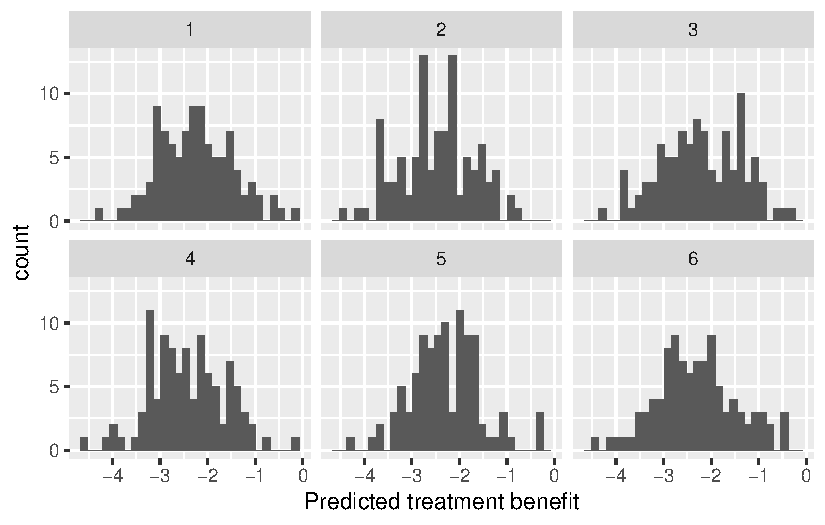
\includegraphics{chapter_16_files/figure-pdf/fig-predben_continuous_outcome-1.pdf}

}

\caption{\label{fig-predben_continuous_outcome}Distribution of predicted
treatment benefit in each trial}

\end{figure}

\hypertarget{penalization}{%
\subsubsection{Penalization}\label{penalization}}

Let us repeat the analysis, but this time while penalizing the
treatment-covariate coefficients using a Bayesian LASSO prior.

\begin{Shaded}
\begin{Highlighting}[]
\NormalTok{ipd }\OtherTok{\textless{}{-}} \FunctionTok{with}\NormalTok{(ds, }\FunctionTok{ipdma.model.onestage}\NormalTok{(}\AttributeTok{y =}\NormalTok{ y, }\AttributeTok{study =}\NormalTok{ studyid, }
                                     \AttributeTok{treat =}\NormalTok{ treat,}
                                     \AttributeTok{X =} \FunctionTok{cbind}\NormalTok{(z1, z2), }
                                     \AttributeTok{response =} \StringTok{"normal"}\NormalTok{, }
                                     \AttributeTok{shrinkage =} \StringTok{"laplace"}\NormalTok{), }
            \AttributeTok{type =} \StringTok{"random"}\NormalTok{)}

\NormalTok{samples }\OtherTok{\textless{}{-}} \FunctionTok{ipd.run}\NormalTok{(ipd, }\AttributeTok{n.chains =} \DecValTok{2}\NormalTok{, }\AttributeTok{n.iter =} \DecValTok{20}\NormalTok{, }
                   \AttributeTok{pars.save =} \FunctionTok{c}\NormalTok{(}\StringTok{"alpha"}\NormalTok{, }\StringTok{"beta"}\NormalTok{, }\StringTok{"delta"}\NormalTok{, }\StringTok{"sd"}\NormalTok{, }\StringTok{"gamma"}\NormalTok{))}
\end{Highlighting}
\end{Shaded}

\begin{verbatim}
Compiling model graph
   Resolving undeclared variables
   Allocating nodes
Graph information:
   Observed stochastic nodes: 600
   Unobserved stochastic nodes: 20
   Total graph size: 6039

Initializing model
\end{verbatim}

\begin{Shaded}
\begin{Highlighting}[]
\FunctionTok{round}\NormalTok{(}\FunctionTok{treatment.effect}\NormalTok{(ipd, samples, }\AttributeTok{newpatient =} \FunctionTok{c}\NormalTok{(}\DecValTok{1}\NormalTok{,}\FloatTok{0.5}\NormalTok{)), }\DecValTok{2}\NormalTok{)}
\end{Highlighting}
\end{Shaded}

\begin{verbatim}
0.025   0.5 0.975 
-5.07 -3.38 -2.45 
\end{verbatim}

\hypertarget{example-of-a-binary-outcome}{%
\subsection{Example of a binary
outcome}\label{example-of-a-binary-outcome}}

\hypertarget{setup-1}{%
\subsubsection{Setup}\label{setup-1}}

We now present the case of a binary outcome. We first generate a dataset
as before, using the \textbf{bipd} package.

\begin{Shaded}
\begin{Highlighting}[]
\NormalTok{ds2 }\OtherTok{\textless{}{-}} \FunctionTok{generate\_ipdma\_example}\NormalTok{(}\AttributeTok{type =} \StringTok{"binary"}\NormalTok{)}
\FunctionTok{head}\NormalTok{(ds2)}
\end{Highlighting}
\end{Shaded}

\begin{verbatim}
  studyid treat         w1           w2 y
1       1     0 -1.2303395  1.386443041 1
2       1     1  0.9995966  0.326715503 0
3       1     0 -1.1008584  1.060149816 0
4       1     1  2.8577405 -0.015462936 0
5       1     1 -1.4637407  0.398844344 0
6       1     0 -0.3153284  0.006682804 0
\end{verbatim}

The simulated dataset contains information on the following variables:

\begin{itemize}
\tightlist
\item
  the trial indicator \texttt{studyid}
\item
  the treatment indicator \texttt{treat}, which takes the values 0 for
  control and 1 for active treatment
\item
  two prognostic variables \texttt{w1} and \texttt{w2}
\item
  the binary outcome \texttt{y}
\end{itemize}

\hypertarget{tbl-summary-binary_outcome-data}{}
\begin{table}
\caption{\label{tbl-summary-binary_outcome-data}The simulated dataset with a binary outcome }\tabularnewline

\centering
\begin{tabular}[t]{llll}
\toprule
  & 0 & 1 & Overall\\
\midrule
 & (N=291) & (N=309) & (N=600)\\
\addlinespace[0.3em]
\multicolumn{4}{l}{\textbf{w1}}\\
\hspace{1em}Mean (SD) & 0.00796 (0.958) & 0.0314 (0.897) & 0.0200 (0.926)\\
\hspace{1em}Median [Min, Max] & -0.00405 [-2.72, 2.78] & 0.0593 [-2.00, 2.86] & 0.0423 [-2.72, 2.86]\\
\addlinespace[0.3em]
\multicolumn{4}{l}{\textbf{w2}}\\
\hspace{1em}Mean (SD) & 0.0459 (1.02) & -0.0446 (1.05) & -0.000697 (1.04)\\
\hspace{1em}Median [Min, Max] & 0.107 [-2.70, 2.68] & -0.0511 [-3.32, 2.67] & 0.000535 [-3.32, 2.68]\\
\addlinespace[0.3em]
\multicolumn{4}{l}{\textbf{studyid}}\\
\hspace{1em}1 & 52 (17.9\%) & 48 (15.5\%) & 100 (16.7\%)\\
\hspace{1em}2 & 45 (15.5\%) & 55 (17.8\%) & 100 (16.7\%)\\
\hspace{1em}3 & 51 (17.5\%) & 49 (15.9\%) & 100 (16.7\%)\\
\hspace{1em}4 & 47 (16.2\%) & 53 (17.2\%) & 100 (16.7\%)\\
\hspace{1em}5 & 45 (15.5\%) & 55 (17.8\%) & 100 (16.7\%)\\
\hspace{1em}6 & 51 (17.5\%) & 49 (15.9\%) & 100 (16.7\%)\\
\bottomrule
\end{tabular}
\end{table}

\hypertarget{model-fitting-1}{%
\subsubsection{Model fitting}\label{model-fitting-1}}

We use a Bayesian random effects model with binomial likelihood. This is
similar to the model 16.7 of the book, but with a Binomial likelihood,
i.e.~

\[ 
y_{ij}\sim Binomial(\pi_{ij}) \\
\] \[ 
logit(\pi_{ij})==a_j+\delta_j t_{ij}+ \sum_{l=1}^{L}\beta_l x_{ij}+ \sum_{l=1}^{L}\gamma_l x_{ij} t_{ij}
\] The remaining of the model is as in the book. We can penalize the
estimated parameters for effect modification (\(\gamma\)'s), using a
Bayesian LASSO. We can do this using again the \emph{bipd} package:

\begin{Shaded}
\begin{Highlighting}[]
\NormalTok{ipd2 }\OtherTok{\textless{}{-}} \FunctionTok{with}\NormalTok{(ds2, }\FunctionTok{ipdma.model.onestage}\NormalTok{(}\AttributeTok{y =}\NormalTok{ y, }\AttributeTok{study =}\NormalTok{ studyid, }\AttributeTok{treat =}\NormalTok{ treat,}
                                       \AttributeTok{X =} \FunctionTok{cbind}\NormalTok{(w1, w2), }
                                       \AttributeTok{response =} \StringTok{"binomial"}\NormalTok{, }
                                       \AttributeTok{shrinkage =} \StringTok{"laplace"}\NormalTok{), }
             \AttributeTok{type=}\StringTok{"random"}\NormalTok{, }\AttributeTok{hy.prior =} \FunctionTok{list}\NormalTok{(}\StringTok{"dunif"}\NormalTok{, }\DecValTok{0}\NormalTok{, }\DecValTok{1}\NormalTok{))}

\NormalTok{ipd2}\SpecialCharTok{$}\NormalTok{model.JAGS}
\end{Highlighting}
\end{Shaded}

\begin{verbatim}
function () 
{
    for (i in 1:Np) {
        y[i] ~ dbern(p[i])
        logit(p[i]) <- alpha[studyid[i]] + inprod(beta[], X[i, 
            ]) + (1 - equals(treat[i], 1)) * inprod(gamma[], 
            X[i, ]) + d[studyid[i], treat[i]]
    }
    for (j in 1:Nstudies) {
        d[j, 1] <- 0
        d[j, 2] ~ dnorm(delta[2], tau)
    }
    sd ~ dnorm(0, 1)
    T(0, )
    tau <- pow(sd, -2)
    delta[1] <- 0
    delta[2] ~ dnorm(0, 0.001)
    for (j in 1:Nstudies) {
        alpha[j] ~ dnorm(0, 0.001)
    }
    for (k in 1:Ncovariate) {
        beta[k] ~ dnorm(0, 0.001)
    }
    tt <- lambda
    lambda <- pow(lambda.inv, -1)
    lambda.inv ~ dunif(0, 5)
    for (k in 1:Ncovariate) {
        gamma[k] ~ ddexp(0, tt)
    }
}
<environment: 0x000002aa847ff3e8>
\end{verbatim}

\begin{Shaded}
\begin{Highlighting}[]
\NormalTok{samples }\OtherTok{\textless{}{-}} \FunctionTok{ipd.run}\NormalTok{(ipd2, }\AttributeTok{n.chains =} \DecValTok{2}\NormalTok{, }\AttributeTok{n.iter =} \DecValTok{20}\NormalTok{, }
                   \AttributeTok{pars.save =} \FunctionTok{c}\NormalTok{(}\StringTok{"alpha"}\NormalTok{, }\StringTok{"beta"}\NormalTok{, }\StringTok{"delta"}\NormalTok{, }\StringTok{"sd"}\NormalTok{, }\StringTok{"gamma"}\NormalTok{))}
\end{Highlighting}
\end{Shaded}

\begin{verbatim}
Compiling model graph
   Resolving undeclared variables
   Allocating nodes
Graph information:
   Observed stochastic nodes: 600
   Unobserved stochastic nodes: 19
   Total graph size: 6637

Initializing model
\end{verbatim}

\begin{Shaded}
\begin{Highlighting}[]
\FunctionTok{summary}\NormalTok{(samples)}
\end{Highlighting}
\end{Shaded}

\begin{verbatim}

Iterations = 2001:2020
Thinning interval = 1 
Number of chains = 2 
Sample size per chain = 20 

1. Empirical mean and standard deviation for each variable,
   plus standard error of the mean:

             Mean     SD Naive SE Time-series SE
alpha[1] -0.34078 0.2776  0.04389        0.06585
alpha[2] -0.80783 0.2718  0.04298        0.07790
alpha[3] -1.19985 0.3202  0.05063        0.08576
alpha[4] -0.85804 0.1990  0.03146        0.04716
alpha[5] -1.06959 0.2987  0.04724        0.10169
alpha[6] -0.94425 0.3131  0.04951        0.07678
beta[1]  -0.03590 0.1000  0.01582        0.01967
beta[2]  -0.03756 0.1218  0.01926        0.02130
delta[1]  0.00000 0.0000  0.00000        0.00000
delta[2] -0.01096 0.4379  0.06924        0.08327
gamma[1]  0.09028 0.1149  0.01816        0.02171
gamma[2]  0.21330 0.1498  0.02368        0.02245
sd        0.78142 0.2498  0.03950        0.07800

2. Quantiles for each variable:

               2.5%      25%      50%      75%   97.5%
alpha[1] -0.7605646 -0.50432 -0.37277 -0.15051  0.2115
alpha[2] -1.1484144 -1.00197 -0.86278 -0.60084 -0.2906
alpha[3] -1.8728435 -1.36581 -1.08526 -0.94346 -0.8677
alpha[4] -1.2660197 -0.99241 -0.81621 -0.74412 -0.5379
alpha[5] -1.6683012 -1.25329 -1.04303 -0.81286 -0.6004
alpha[6] -1.4772417 -1.16204 -0.92320 -0.84119 -0.3009
beta[1]  -0.2363999 -0.07803 -0.01780  0.03226  0.1232
beta[2]  -0.2262688 -0.13719 -0.04790  0.06893  0.1935
delta[1]  0.0000000  0.00000  0.00000  0.00000  0.0000
delta[2] -0.9416291 -0.24785  0.02087  0.23443  0.7910
gamma[1] -0.1021983  0.01017  0.09435  0.19198  0.2604
gamma[2]  0.0006925  0.10911  0.22227  0.29650  0.4860
sd        0.4516838  0.58578  0.74924  0.94277  1.2447
\end{verbatim}

\begin{Shaded}
\begin{Highlighting}[]
\FunctionTok{round}\NormalTok{(}\FunctionTok{treatment.effect}\NormalTok{(ipd2, samples, }\AttributeTok{newpatient =} \FunctionTok{c}\NormalTok{(}\AttributeTok{w1=} \FloatTok{1.6}\NormalTok{, }\AttributeTok{w2 =} \FloatTok{1.3}\NormalTok{)), }\DecValTok{2}\NormalTok{)}
\end{Highlighting}
\end{Shaded}

\begin{verbatim}
0.025   0.5 0.975 
 0.59  1.65  3.32 
\end{verbatim}

\hypertarget{estimating-heterogeous-treatment-effects-in-network-meta-analysis}{%
\section{Estimating heterogeous treatment effects in network
meta-analysis}\label{estimating-heterogeous-treatment-effects-in-network-meta-analysis}}

\hypertarget{example-of-a-continuous-outcome-1}{%
\subsection{Example of a continuous
outcome}\label{example-of-a-continuous-outcome-1}}

\hypertarget{setup-2}{%
\subsubsection{Setup}\label{setup-2}}

We use again the bipd package to simulate a dataset:

\begin{Shaded}
\begin{Highlighting}[]
\NormalTok{ds3 }\OtherTok{\textless{}{-}} \FunctionTok{generate\_ipdnma\_example}\NormalTok{(}\AttributeTok{type =} \StringTok{"continuous"}\NormalTok{)}
\FunctionTok{head}\NormalTok{(ds3)}
\end{Highlighting}
\end{Shaded}

\begin{verbatim}
  studyid treat         z1         z2  y
1       1     1  0.1829614 -0.3583425 11
2       1     1 -1.3498681 -0.4742485 11
3       1     1 -0.6371446  0.8219166 11
4       1     2 -2.2352659 -1.6490255  8
5       1     2  0.1722712  1.3452323  9
6       1     2  1.9461896  1.1121450  8
\end{verbatim}

Let us look into the data a bit in more detail:

\hypertarget{tbl-nma-summary-continuous_outcome-data}{}
\begin{table}
\caption{\label{tbl-nma-summary-continuous_outcome-data}The simulated dataset with a continuous outcome }\tabularnewline

\centering
\begin{tabular}[t]{lllll}
\toprule
  & 1 & 2 & 3 & Overall\\
\midrule
 & (N=349) & (N=355) & (N=296) & (N=1000)\\
\addlinespace[0.3em]
\multicolumn{5}{l}{\textbf{z1}}\\
\hspace{1em}Mean (SD) & -0.0323 (1.00) & 0.0113 (0.996) & -0.0787 (0.958) & -0.0306 (0.987)\\
\hspace{1em}Median [Min, Max] & -0.0262 [-3.17, 2.69] & -0.0127 [-2.67, 3.78] & -0.0860 [-2.41, 2.47] & -0.0318 [-3.17, 3.78]\\
\addlinespace[0.3em]
\multicolumn{5}{l}{\textbf{z2}}\\
\hspace{1em}Mean (SD) & -0.0524 (0.981) & -0.0161 (1.02) & -0.0959 (1.05) & -0.0524 (1.02)\\
\hspace{1em}Median [Min, Max] & -0.0323 [-2.69, 2.55] & -0.0175 [-3.32, 2.95] & -0.139 [-3.14, 2.34] & -0.0511 [-3.32, 2.95]\\
\addlinespace[0.3em]
\multicolumn{5}{l}{\textbf{studyid}}\\
\hspace{1em}1 & 46 (13.2\%) & 54 (15.2\%) & 0 (0\%) & 100 (10.0\%)\\
\hspace{1em}2 & 46 (13.2\%) & 54 (15.2\%) & 0 (0\%) & 100 (10.0\%)\\
\hspace{1em}3 & 50 (14.3\%) & 50 (14.1\%) & 0 (0\%) & 100 (10.0\%)\\
\hspace{1em}4 & 54 (15.5\%) & 0 (0\%) & 46 (15.5\%) & 100 (10.0\%)\\
\hspace{1em}5 & 47 (13.5\%) & 0 (0\%) & 53 (17.9\%) & 100 (10.0\%)\\
\hspace{1em}6 & 0 (0\%) & 42 (11.8\%) & 58 (19.6\%) & 100 (10.0\%)\\
\hspace{1em}7 & 0 (0\%) & 53 (14.9\%) & 47 (15.9\%) & 100 (10.0\%)\\
\hspace{1em}8 & 40 (11.5\%) & 38 (10.7\%) & 22 (7.4\%) & 100 (10.0\%)\\
\hspace{1em}9 & 37 (10.6\%) & 27 (7.6\%) & 36 (12.2\%) & 100 (10.0\%)\\
\hspace{1em}10 & 29 (8.3\%) & 37 (10.4\%) & 34 (11.5\%) & 100 (10.0\%)\\
\bottomrule
\end{tabular}
\end{table}

\hypertarget{model-fitting-2}{%
\subsubsection{Model fitting}\label{model-fitting-2}}

We will use the model shown in Equation 16.8 in the book. In addition,
we will use Bayesian LASSO to penalize the treatment-covariate
interactions.

\begin{Shaded}
\begin{Highlighting}[]
\NormalTok{ipd3 }\OtherTok{\textless{}{-}} \FunctionTok{with}\NormalTok{(ds3, }\FunctionTok{ipdnma.model.onestage}\NormalTok{(}\AttributeTok{y =}\NormalTok{ y, }\AttributeTok{study =}\NormalTok{ studyid, }\AttributeTok{treat =}\NormalTok{ treat, }
                                        \AttributeTok{X =} \FunctionTok{cbind}\NormalTok{(z1, z2), }
                                        \AttributeTok{response =} \StringTok{"normal"}\NormalTok{, }
                                        \AttributeTok{shrinkage =} \StringTok{"laplace"}\NormalTok{, }
                                        \AttributeTok{type =} \StringTok{"random"}\NormalTok{))}
\NormalTok{ipd3}\SpecialCharTok{$}\NormalTok{model.JAGS}
\end{Highlighting}
\end{Shaded}

\begin{verbatim}
function () 
{
    for (i in 1:Np) {
        y[i] ~ dnorm(mu[i], sigma)
        mu[i] <- alpha[studyid[i]] + inprod(beta[], X[i, ]) + 
            inprod(gamma[treat[i], ], X[i, ]) + d[studyid[i], 
            treatment.arm[i]]
    }
    sigma ~ dgamma(0.001, 0.001)
    for (i in 1:Nstudies) {
        w[i, 1] <- 0
        d[i, 1] <- 0
        for (k in 2:na[i]) {
            d[i, k] ~ dnorm(mdelta[i, k], taudelta[i, k])
            mdelta[i, k] <- delta[t[i, k]] - delta[t[i, 1]] + 
                sw[i, k]
            taudelta[i, k] <- tau * 2 * (k - 1)/k
            w[i, k] <- d[i, k] - delta[t[i, k]] + delta[t[i, 
                1]]
            sw[i, k] <- sum(w[i, 1:(k - 1)])/(k - 1)
        }
    }
    sd ~ dnorm(0, 1)
    T(0, )
    tau <- pow(sd, -2)
    delta[1] <- 0
    for (k in 2:Ntreat) {
        delta[k] ~ dnorm(0, 0.001)
    }
    for (j in 1:Nstudies) {
        alpha[j] ~ dnorm(0, 0.001)
    }
    for (k in 1:Ncovariate) {
        beta[k] ~ dnorm(0, 0.001)
    }
    lambda[1] <- 0
    lambda.inv[1] <- 0
    for (m in 2:Ntreat) {
        tt[m] <- lambda[m] * sigma
        lambda[m] <- pow(lambda.inv[m], -1)
        lambda.inv[m] ~ dunif(0, 5)
    }
    for (k in 1:Ncovariate) {
        gamma[1, k] <- 0
        for (m in 2:Ntreat) {
            gamma[m, k] ~ ddexp(0, tt[m])
        }
    }
}
<environment: 0x000002aa855142f8>
\end{verbatim}

\begin{Shaded}
\begin{Highlighting}[]
\NormalTok{samples }\OtherTok{\textless{}{-}} \FunctionTok{ipd.run}\NormalTok{(ipd3, }\AttributeTok{n.chains =} \DecValTok{2}\NormalTok{, }\AttributeTok{n.iter =} \DecValTok{20}\NormalTok{, }
                   \AttributeTok{pars.save =} \FunctionTok{c}\NormalTok{(}\StringTok{"alpha"}\NormalTok{, }\StringTok{"beta"}\NormalTok{, }\StringTok{"delta"}\NormalTok{, }\StringTok{"sd"}\NormalTok{, }\StringTok{"gamma"}\NormalTok{))}
\end{Highlighting}
\end{Shaded}

\begin{verbatim}
Compiling model graph
   Resolving undeclared variables
   Allocating nodes
Graph information:
   Observed stochastic nodes: 1000
   Unobserved stochastic nodes: 35
   Total graph size: 10141

Initializing model
\end{verbatim}

\begin{Shaded}
\begin{Highlighting}[]
\FunctionTok{summary}\NormalTok{(samples)}
\end{Highlighting}
\end{Shaded}

\begin{verbatim}

Iterations = 2001:2020
Thinning interval = 1 
Number of chains = 2 
Sample size per chain = 20 

1. Empirical mean and standard deviation for each variable,
   plus standard error of the mean:

              Mean      SD Naive SE Time-series SE
alpha[1]   11.0143 0.05351 0.008461       0.012893
alpha[2]    8.0104 0.04313 0.006819       0.011318
alpha[3]   10.5057 0.04685 0.007408       0.007344
alpha[4]    9.5642 0.04372 0.006912       0.006977
alpha[5]   12.9822 0.03072 0.004858       0.004887
alpha[6]   13.2670 0.04836 0.007646       0.012434
alpha[7]    7.3961 0.05204 0.008228       0.014720
alpha[8]   11.1075 0.05268 0.008330       0.013409
alpha[9]   10.1329 0.05067 0.008012       0.014126
alpha[10]   9.1592 0.05562 0.008795       0.017214
beta[1]     0.2287 0.01429 0.002259       0.004478
beta[2]     0.3171 0.01742 0.002755       0.005921
delta[1]    0.0000 0.00000 0.000000       0.000000
delta[2]   -2.9582 0.06936 0.010967       0.009455
delta[3]   -1.1239 0.07083 0.011200       0.009991
gamma[1,1]  0.0000 0.00000 0.000000       0.000000
gamma[2,1] -0.6453 0.02223 0.003516       0.006829
gamma[3,1] -0.3277 0.01879 0.002971       0.003337
gamma[1,2]  0.0000 0.00000 0.000000       0.000000
gamma[2,2]  0.6075 0.02498 0.003950       0.007017
gamma[3,2]  0.4135 0.01868 0.002954       0.006306
sd          0.2230 0.05817 0.009198       0.016080

2. Quantiles for each variable:

              2.5%     25%     50%     75%   97.5%
alpha[1]   10.9302 10.9823 11.0220 11.0479 11.0988
alpha[2]    7.9224  7.9816  8.0152  8.0369  8.0830
alpha[3]   10.4128 10.4722 10.5106 10.5439 10.5787
alpha[4]    9.4920  9.5290  9.5637  9.5982  9.6411
alpha[5]   12.9236 12.9621 12.9842 13.0013 13.0324
alpha[6]   13.1556 13.2396 13.2700 13.2984 13.3439
alpha[7]    7.3262  7.3548  7.3923  7.4279  7.4879
alpha[8]   11.0004 11.0811 11.1067 11.1433 11.1924
alpha[9]   10.0257 10.1025 10.1393 10.1667 10.2160
alpha[10]   9.0730  9.1219  9.1572  9.1931  9.2463
beta[1]     0.2016  0.2203  0.2293  0.2358  0.2587
beta[2]     0.2853  0.3059  0.3196  0.3301  0.3481
delta[1]    0.0000  0.0000  0.0000  0.0000  0.0000
delta[2]   -3.1027 -3.0003 -2.9579 -2.9084 -2.8760
delta[3]   -1.2442 -1.1743 -1.1340 -1.0820 -0.9850
gamma[1,1]  0.0000  0.0000  0.0000  0.0000  0.0000
gamma[2,1] -0.6915 -0.6579 -0.6452 -0.6310 -0.6087
gamma[3,1] -0.3700 -0.3387 -0.3263 -0.3166 -0.2969
gamma[1,2]  0.0000  0.0000  0.0000  0.0000  0.0000
gamma[2,2]  0.5617  0.5949  0.6061  0.6285  0.6471
gamma[3,2]  0.3834  0.4000  0.4137  0.4247  0.4442
sd          0.1428  0.1828  0.2184  0.2439  0.3889
\end{verbatim}

As before, we can use the \texttt{treatment.effect()} function of
\emph{bipd} to estimate relative effects for new patients.

\begin{Shaded}
\begin{Highlighting}[]
\FunctionTok{treatment.effect}\NormalTok{(ipd3, samples, }\AttributeTok{newpatient=} \FunctionTok{c}\NormalTok{(}\DecValTok{1}\NormalTok{,}\DecValTok{2}\NormalTok{))}
\end{Highlighting}
\end{Shaded}

\begin{verbatim}
$`treatment 2`
    0.025       0.5     0.975 
-2.525064 -2.418394 -2.266426 

$`treatment 3`
     0.025        0.5      0.975 
-0.7388297 -0.6376228 -0.5007683 
\end{verbatim}

This gives us the relative effects for all treatments versus the
reference. To obtain relative effects between active treatments we need
some more coding:

\begin{Shaded}
\begin{Highlighting}[]
\NormalTok{samples.all}\OtherTok{=}\FunctionTok{data.frame}\NormalTok{(}\FunctionTok{rbind}\NormalTok{(samples[[}\DecValTok{1}\NormalTok{]], samples[[}\DecValTok{2}\NormalTok{]]))}
\NormalTok{newpatient}\OtherTok{=} \FunctionTok{c}\NormalTok{(}\DecValTok{1}\NormalTok{,}\DecValTok{2}\NormalTok{)}
\NormalTok{newpatient }\OtherTok{\textless{}{-}}\NormalTok{ (newpatient }\SpecialCharTok{{-}}\NormalTok{ ipd3}\SpecialCharTok{$}\NormalTok{scale\_mean)}\SpecialCharTok{/}\NormalTok{ipd3}\SpecialCharTok{$}\NormalTok{scale\_sd}

\FunctionTok{median}\NormalTok{(}
\NormalTok{  samples.all}\SpecialCharTok{$}\NormalTok{delta.}\FloatTok{2.}\SpecialCharTok{+}\NormalTok{samples.all}\SpecialCharTok{$}\NormalTok{gamma.}\DecValTok{2}\NormalTok{.}\FloatTok{1.}\SpecialCharTok{*}
\NormalTok{    newpatient[}\DecValTok{1}\NormalTok{]}\SpecialCharTok{+}\NormalTok{samples.all}\SpecialCharTok{$}\NormalTok{gamma.}\DecValTok{2}\NormalTok{.}\FloatTok{2.}\SpecialCharTok{*}\NormalTok{newpatient[}\DecValTok{2}\NormalTok{]}
\SpecialCharTok{{-}}
\NormalTok{  (samples.all}\SpecialCharTok{$}\NormalTok{delta.}\FloatTok{3.}\SpecialCharTok{+}\NormalTok{samples.all}\SpecialCharTok{$}\NormalTok{gamma.}\DecValTok{3}\NormalTok{.}\FloatTok{1.}\SpecialCharTok{*}\NormalTok{newpatient[}\DecValTok{1}\NormalTok{]}\SpecialCharTok{+}
\NormalTok{     samples.all}\SpecialCharTok{$}\NormalTok{gamma.}\DecValTok{3}\NormalTok{.}\FloatTok{2.}\SpecialCharTok{*}\NormalTok{newpatient[}\DecValTok{2}\NormalTok{])}
\NormalTok{)}
\end{Highlighting}
\end{Shaded}

\begin{verbatim}
[1] -1.765342
\end{verbatim}

\begin{Shaded}
\begin{Highlighting}[]
\FunctionTok{quantile}\NormalTok{(samples.all}\SpecialCharTok{$}\NormalTok{delta.}\FloatTok{2.}\SpecialCharTok{+}\NormalTok{samples.all}\SpecialCharTok{$}\NormalTok{gamma.}\DecValTok{2}\NormalTok{.}\FloatTok{1.}\SpecialCharTok{*}
\NormalTok{           newpatient[}\DecValTok{1}\NormalTok{]}\SpecialCharTok{+}\NormalTok{samples.all}\SpecialCharTok{$}\NormalTok{gamma.}\DecValTok{2}\NormalTok{.}\FloatTok{2.}\SpecialCharTok{*}\NormalTok{newpatient[}\DecValTok{2}\NormalTok{]}
         \SpecialCharTok{{-}}\NormalTok{(samples.all}\SpecialCharTok{$}\NormalTok{delta.}\FloatTok{3.}\SpecialCharTok{+}\NormalTok{samples.all}\SpecialCharTok{$}\NormalTok{gamma.}\DecValTok{3}\NormalTok{.}\FloatTok{1.}\SpecialCharTok{*}\NormalTok{newpatient[}\DecValTok{1}\NormalTok{]}\SpecialCharTok{+}
\NormalTok{             samples.all}\SpecialCharTok{$}\NormalTok{gamma.}\DecValTok{3}\NormalTok{.}\FloatTok{2.}\SpecialCharTok{*}\NormalTok{newpatient[}\DecValTok{2}\NormalTok{])}
\NormalTok{         , }\AttributeTok{probs =} \FloatTok{0.025}\NormalTok{)}
\end{Highlighting}
\end{Shaded}

\begin{verbatim}
     2.5% 
-1.940397 
\end{verbatim}

\begin{Shaded}
\begin{Highlighting}[]
\FunctionTok{quantile}\NormalTok{(samples.all}\SpecialCharTok{$}\NormalTok{delta.}\FloatTok{2.}\SpecialCharTok{+}\NormalTok{samples.all}\SpecialCharTok{$}\NormalTok{gamma.}\DecValTok{2}\NormalTok{.}\FloatTok{1.}\SpecialCharTok{*}
\NormalTok{           newpatient[}\DecValTok{1}\NormalTok{]}\SpecialCharTok{+}\NormalTok{samples.all}\SpecialCharTok{$}\NormalTok{gamma.}\DecValTok{2}\NormalTok{.}\FloatTok{2.}\SpecialCharTok{*}\NormalTok{newpatient[}\DecValTok{2}\NormalTok{]}
         \SpecialCharTok{{-}}\NormalTok{(samples.all}\SpecialCharTok{$}\NormalTok{delta.}\FloatTok{3.}\SpecialCharTok{+}\NormalTok{samples.all}\SpecialCharTok{$}\NormalTok{gamma.}\DecValTok{3}\NormalTok{.}\FloatTok{1.}\SpecialCharTok{*}\NormalTok{newpatient[}\DecValTok{1}\NormalTok{]}\SpecialCharTok{+}
\NormalTok{             samples.all}\SpecialCharTok{$}\NormalTok{gamma.}\DecValTok{3}\NormalTok{.}\FloatTok{2.}\SpecialCharTok{*}\NormalTok{newpatient[}\DecValTok{2}\NormalTok{])}
\NormalTok{         , }\AttributeTok{probs =} \FloatTok{0.975}\NormalTok{)}
\end{Highlighting}
\end{Shaded}

\begin{verbatim}
   97.5% 
-1.62695 
\end{verbatim}

\hypertarget{modeling-patient-level-relative-effects-using-randomized-and-observational-evidence-for-a-network-of-treatments}{%
\subsection{Modeling patient-level relative effects using randomized and
observational evidence for a network of
treatments}\label{modeling-patient-level-relative-effects-using-randomized-and-observational-evidence-for-a-network-of-treatments}}

We will now follow Chapter 16.3.5 from the book. In this analysis we
will not use penalization, and we will assume fixed effects. For an
example with penalization and random effects, see part 2 of this
vignettte.

\hypertarget{setup-3}{%
\subsubsection{Setup}\label{setup-3}}

We generate a very simple dataset of three studies comparing three
treatments. We will assume 2 RCTs and 1 non-randomized trial:

\begin{Shaded}
\begin{Highlighting}[]
\NormalTok{ds4 }\OtherTok{\textless{}{-}} \FunctionTok{generate\_ipdnma\_example}\NormalTok{(}\AttributeTok{type =} \StringTok{"continuous"}\NormalTok{)}
\NormalTok{ds4 }\OtherTok{\textless{}{-}}\NormalTok{ ds4 }\SpecialCharTok{\%\textgreater{}\%} \FunctionTok{filter}\NormalTok{(studyid }\SpecialCharTok{\%in\%} \FunctionTok{c}\NormalTok{(}\DecValTok{1}\NormalTok{,}\DecValTok{4}\NormalTok{,}\DecValTok{10}\NormalTok{)) }\SpecialCharTok{\%\textgreater{}\%}
  \FunctionTok{mutate}\NormalTok{(}\AttributeTok{studyid =} \FunctionTok{factor}\NormalTok{(studyid) }\SpecialCharTok{\%\textgreater{}\%}
           \FunctionTok{recode\_factor}\NormalTok{(}
             \StringTok{"1"} \OtherTok{=} \StringTok{"1"}\NormalTok{,}
             \StringTok{"4"} \OtherTok{=} \StringTok{"2"}\NormalTok{,}
             \StringTok{"10"} \OtherTok{=} \StringTok{"3"}\NormalTok{),}
         \AttributeTok{design =} \FunctionTok{ifelse}\NormalTok{(studyid }\SpecialCharTok{==} \StringTok{"3"}\NormalTok{, }\StringTok{"nrs"}\NormalTok{, }\StringTok{"rct"}\NormalTok{))}
\end{Highlighting}
\end{Shaded}

The sample size is as follows:

\begin{verbatim}
          
           s1 s2 s3
  treat A: 41 51 39
  treat B: 59  0 25
  treat C:  0 49 36
\end{verbatim}

\hypertarget{model-fitting-3}{%
\subsubsection{Model fitting}\label{model-fitting-3}}

We will use the design-adjusted model, equation 16.9 in the book. We
will fit a two-stage fixed effects meta-analysis and we will use a
variance inflation factor. The code below is used to specify the
analysis of each individual study. Briefly, in each study we adjust the
treatment effect for the prognostic factors \texttt{z1} and \texttt{z2},
as well as their interaction with \texttt{treat}.

\begin{Shaded}
\begin{Highlighting}[]
\FunctionTok{library}\NormalTok{(rjags)}
\end{Highlighting}
\end{Shaded}

\begin{verbatim}
Loading required package: coda
\end{verbatim}

\begin{verbatim}
Linked to JAGS 4.3.1
\end{verbatim}

\begin{verbatim}
Loaded modules: basemod,bugs
\end{verbatim}

\begin{Shaded}
\begin{Highlighting}[]
\NormalTok{first.stage }\OtherTok{\textless{}{-}} \StringTok{"}
\StringTok{model\{}

\StringTok{for (i in 1:N)\{}
\StringTok{    y[i] \textasciitilde{} dnorm(mu[i], tau)  }
\StringTok{    mu[i] \textless{}{-} a + inprod(b[], X[i,]) + inprod(c[,treat[i]], X[i,]) + d[treat[i]] }
\StringTok{\}}
\StringTok{sigma \textasciitilde{} dunif(0, 5)}
\StringTok{tau \textless{}{-} pow(sigma, {-}2)}

\StringTok{a \textasciitilde{} dnorm(0, 0.001)}

\StringTok{for(k in 1:Ncovariate)\{}
\StringTok{    b[k] \textasciitilde{} dnorm(0,0.001)}
\StringTok{\}}

\StringTok{for(k in 1:Ncovariate)\{}
\StringTok{    c[k,1] \textless{}{-} 0}
\StringTok{\}}

\StringTok{tauGamma \textless{}{-} pow(sdGamma,{-}1)}
\StringTok{sdGamma \textasciitilde{} dunif(0, 5)}

\StringTok{for(k in 1:Ncovariate)\{}
\StringTok{    for(t in 2:Ntreat)\{}
\StringTok{        c[k,t] \textasciitilde{} ddexp(0, tauGamma)}
\StringTok{    \}}
\StringTok{\}}

\StringTok{d[1] \textless{}{-} 0}
\StringTok{for(t in 2:Ntreat)\{}
\StringTok{    d[t] \textasciitilde{} dnorm(0, 0.001)}
\StringTok{\}}
\StringTok{\}"}
\end{Highlighting}
\end{Shaded}

Subsequently, we estimate the relative treatment effects in the first
(randomized) study comparing treatments A and B:

\begin{Shaded}
\begin{Highlighting}[]
\NormalTok{model1.spec }\OtherTok{\textless{}{-}} \FunctionTok{textConnection}\NormalTok{(first.stage) }
\NormalTok{data1 }\OtherTok{\textless{}{-}} \FunctionTok{with}\NormalTok{(ds4 }\SpecialCharTok{\%\textgreater{}\%} \FunctionTok{filter}\NormalTok{(studyid }\SpecialCharTok{==} \DecValTok{1}\NormalTok{), }
              \FunctionTok{list}\NormalTok{(}\AttributeTok{y =}\NormalTok{ y,}
                   \AttributeTok{N =} \FunctionTok{length}\NormalTok{(y), }
                   \AttributeTok{X =} \FunctionTok{cbind}\NormalTok{(z1,z2),  }
                   \AttributeTok{treat =}\NormalTok{ treat,}
                   \AttributeTok{Ncovariate =} \DecValTok{2}\NormalTok{, }
                   \AttributeTok{Ntreat =} \DecValTok{2}\NormalTok{))}
\NormalTok{jags.m }\OtherTok{\textless{}{-}} \FunctionTok{jags.model}\NormalTok{(model1.spec, }\AttributeTok{data =}\NormalTok{ data1, }\AttributeTok{n.chains =} \DecValTok{2}\NormalTok{, }\AttributeTok{n.adapt =} \DecValTok{500}\NormalTok{,}
                     \AttributeTok{quiet =}  \ConstantTok{TRUE}\NormalTok{)}
\NormalTok{params }\OtherTok{\textless{}{-}} \FunctionTok{c}\NormalTok{(}\StringTok{"d"}\NormalTok{, }\StringTok{"c"}\NormalTok{) }
\NormalTok{samps4}\FloatTok{.1} \OtherTok{\textless{}{-}} \FunctionTok{coda.samples}\NormalTok{(jags.m, params, }\AttributeTok{n.iter =} \DecValTok{50}\NormalTok{)}
\NormalTok{samps.all.s1 }\OtherTok{\textless{}{-}} \FunctionTok{data.frame}\NormalTok{(}\FunctionTok{as.matrix}\NormalTok{(samps4}\FloatTok{.1}\NormalTok{))}

\NormalTok{samps.all.s1 }\OtherTok{\textless{}{-}}\NormalTok{ samps.all.s1[, }\FunctionTok{c}\NormalTok{(}\StringTok{"c.1.2."}\NormalTok{, }\StringTok{"c.2.2."}\NormalTok{, }\StringTok{"d.2."}\NormalTok{)]}
\NormalTok{delta}\FloatTok{.1} \OtherTok{\textless{}{-}} \FunctionTok{colMeans}\NormalTok{(samps.all.s1)}
\NormalTok{cov}\FloatTok{.1} \OtherTok{\textless{}{-}} \FunctionTok{var}\NormalTok{(samps.all.s1)}
\end{Highlighting}
\end{Shaded}

We repeat the analysis for the second (randomized) study comparing
treatments A and C:

\begin{Shaded}
\begin{Highlighting}[]
\NormalTok{model1.spec }\OtherTok{\textless{}{-}} \FunctionTok{textConnection}\NormalTok{(first.stage) }
\NormalTok{data2 }\OtherTok{\textless{}{-}} \FunctionTok{with}\NormalTok{(ds4 }\SpecialCharTok{\%\textgreater{}\%} \FunctionTok{filter}\NormalTok{(studyid }\SpecialCharTok{==} \DecValTok{2}\NormalTok{), }
              \FunctionTok{list}\NormalTok{(}\AttributeTok{y =}\NormalTok{ y,}
                   \AttributeTok{N =} \FunctionTok{length}\NormalTok{(y), }
                   \AttributeTok{X =} \FunctionTok{cbind}\NormalTok{(z1,z2),  }
                   \AttributeTok{treat =} \FunctionTok{ifelse}\NormalTok{(treat }\SpecialCharTok{==} \DecValTok{3}\NormalTok{, }\DecValTok{2}\NormalTok{, treat),}
                   \AttributeTok{Ncovariate =} \DecValTok{2}\NormalTok{, }
                   \AttributeTok{Ntreat =} \DecValTok{2}\NormalTok{))}
\NormalTok{jags.m }\OtherTok{\textless{}{-}} \FunctionTok{jags.model}\NormalTok{(model1.spec, }\AttributeTok{data =}\NormalTok{ data2, }\AttributeTok{n.chains =} \DecValTok{2}\NormalTok{, }\AttributeTok{n.adapt =} \DecValTok{100}\NormalTok{,}
                     \AttributeTok{quiet =}  \ConstantTok{TRUE}\NormalTok{)}
\NormalTok{params }\OtherTok{\textless{}{-}} \FunctionTok{c}\NormalTok{(}\StringTok{"d"}\NormalTok{, }\StringTok{"c"}\NormalTok{) }
\NormalTok{samps4}\FloatTok{.2} \OtherTok{\textless{}{-}} \FunctionTok{coda.samples}\NormalTok{(jags.m, params, }\AttributeTok{n.iter =} \DecValTok{50}\NormalTok{)}
\NormalTok{samps.all.s2 }\OtherTok{\textless{}{-}} \FunctionTok{data.frame}\NormalTok{(}\FunctionTok{as.matrix}\NormalTok{(samps4}\FloatTok{.2}\NormalTok{))}
\NormalTok{samps.all.s2 }\OtherTok{\textless{}{-}}\NormalTok{ samps.all.s2[, }\FunctionTok{c}\NormalTok{(}\StringTok{"c.1.2."}\NormalTok{, }\StringTok{"c.2.2."}\NormalTok{, }\StringTok{"d.2."}\NormalTok{)]}
\NormalTok{delta}\FloatTok{.2} \OtherTok{\textless{}{-}} \FunctionTok{colMeans}\NormalTok{(samps.all.s2)}
\NormalTok{cov}\FloatTok{.2} \OtherTok{\textless{}{-}} \FunctionTok{var}\NormalTok{(samps.all.s2)}
\end{Highlighting}
\end{Shaded}

Finally, we analyze the third (non-randomized) study comparing
treatments A, B, and C:

\begin{Shaded}
\begin{Highlighting}[]
\NormalTok{model1.spec }\OtherTok{\textless{}{-}} \FunctionTok{textConnection}\NormalTok{(first.stage) }
\NormalTok{data3 }\OtherTok{\textless{}{-}} \FunctionTok{with}\NormalTok{(ds4 }\SpecialCharTok{\%\textgreater{}\%} \FunctionTok{filter}\NormalTok{(studyid }\SpecialCharTok{==} \DecValTok{3}\NormalTok{), }
              \FunctionTok{list}\NormalTok{(}\AttributeTok{y =}\NormalTok{ y,}
                   \AttributeTok{N =} \FunctionTok{length}\NormalTok{(y), }
                   \AttributeTok{X =} \FunctionTok{cbind}\NormalTok{(z1,z2),  }
                   \AttributeTok{treat =}\NormalTok{ treat,}
                   \AttributeTok{Ncovariate =} \DecValTok{2}\NormalTok{, }
                   \AttributeTok{Ntreat =} \DecValTok{3}\NormalTok{))}
\NormalTok{jags.m }\OtherTok{\textless{}{-}} \FunctionTok{jags.model}\NormalTok{(model1.spec, }\AttributeTok{data =}\NormalTok{ data3, }\AttributeTok{n.chains =} \DecValTok{2}\NormalTok{, }\AttributeTok{n.adapt =} \DecValTok{100}\NormalTok{,}
                     \AttributeTok{quiet =} \ConstantTok{TRUE}\NormalTok{)}
\NormalTok{params }\OtherTok{\textless{}{-}} \FunctionTok{c}\NormalTok{(}\StringTok{"d"}\NormalTok{, }\StringTok{"c"}\NormalTok{) }
\NormalTok{samps4}\FloatTok{.3} \OtherTok{\textless{}{-}} \FunctionTok{coda.samples}\NormalTok{(jags.m, params, }\AttributeTok{n.iter =} \DecValTok{50}\NormalTok{)}
\NormalTok{samps.all.s3 }\OtherTok{\textless{}{-}} \FunctionTok{data.frame}\NormalTok{(}\FunctionTok{as.matrix}\NormalTok{(samps4}\FloatTok{.3}\NormalTok{))}

\NormalTok{samps.all.s3 }\OtherTok{\textless{}{-}}\NormalTok{ samps.all.s3[, }\FunctionTok{c}\NormalTok{(}\StringTok{"c.1.2."}\NormalTok{, }\StringTok{"c.2.2."}\NormalTok{, }\StringTok{"d.2."}\NormalTok{, }\StringTok{"c.1.3."}\NormalTok{, }
                                 \StringTok{"c.2.3."}\NormalTok{, }\StringTok{"d.3."}\NormalTok{)]}
\NormalTok{delta}\FloatTok{.3} \OtherTok{\textless{}{-}} \FunctionTok{colMeans}\NormalTok{(samps.all.s3)}
\NormalTok{cov}\FloatTok{.3} \OtherTok{\textless{}{-}} \FunctionTok{var}\NormalTok{(samps.all.s3)}
\end{Highlighting}
\end{Shaded}

The corresponding treatment effect estimates are depicted below:

\hypertarget{tbl-results_nma_stage1}{}
\begin{table}[!h]
\caption{\label{tbl-results_nma_stage1}Treatment effect estimates. }\tabularnewline

\centering
\begin{tabular}{lll}
\toprule
study & B versus A & C versus A\\
\midrule
study 1 & -3.012 (SE =  0.062 ) & \\
study 2 &  & -1.228 (SE =  0.051 )\\
study 3 & -3.013 (SE =  0.082 ) & -1.052 (SE =  0.073 )\\
\bottomrule
\end{tabular}
\end{table}

We can now fit the second stage of the network meta-analysis. The
corresponding JAGS model is specified below:

\begin{Shaded}
\begin{Highlighting}[]
\NormalTok{second.stage }\OtherTok{\textless{}{-}}
\StringTok{"model\{}
\StringTok{  }
\StringTok{  \#likelihood}
\StringTok{  y1 \textasciitilde{} dmnorm(Mu1, Omega1)}
\StringTok{  y2 \textasciitilde{} dmnorm(Mu2, Omega2)}
\StringTok{  y3 \textasciitilde{} dmnorm(Mu3, Omega3*W)}

\StringTok{  }
\StringTok{  Omega1 \textless{}{-} inverse(cov.1)}
\StringTok{  Omega2 \textless{}{-} inverse(cov.2)}
\StringTok{  Omega3 \textless{}{-} inverse(cov.3)}

\StringTok{  Mu1 \textless{}{-} c(gamma[,1], delta[2])}
\StringTok{  Mu2 \textless{}{-} c(gamma[,2], delta[3])  }
\StringTok{  Mu3 \textless{}{-} c(gamma[,1], delta[2],gamma[,2], delta[3])}
\StringTok{  }
\StringTok{  \#parameters}
\StringTok{  for(i in 1:2)\{}
\StringTok{    gamma[i,1] \textasciitilde{} dnorm(0, 0.001)}
\StringTok{    gamma[i,2] \textasciitilde{} dnorm(0, 0.001)}
\StringTok{  \}}
\StringTok{  }
\StringTok{  delta[1] \textless{}{-} 0}
\StringTok{  delta[2] \textasciitilde{} dnorm(0, 0.001)}
\StringTok{  delta[3] \textasciitilde{} dnorm(0, 0.001)}
\StringTok{  }
\StringTok{\}}
\StringTok{"}
\end{Highlighting}
\end{Shaded}

We can fit as follows:

\begin{Shaded}
\begin{Highlighting}[]
\NormalTok{model1.spec }\OtherTok{\textless{}{-}} \FunctionTok{textConnection}\NormalTok{(second.stage) }
\NormalTok{data3 }\OtherTok{\textless{}{-}} \FunctionTok{list}\NormalTok{(}\AttributeTok{y1 =}\NormalTok{ delta}\FloatTok{.1}\NormalTok{, }\AttributeTok{y2 =}\NormalTok{ delta}\FloatTok{.2}\NormalTok{, }\AttributeTok{y3 =}\NormalTok{ delta}\FloatTok{.3}\NormalTok{, }
              \AttributeTok{cov.1 =}\NormalTok{ cov}\FloatTok{.1}\NormalTok{, }\AttributeTok{cov.2 =}\NormalTok{ cov}\FloatTok{.2}\NormalTok{, }\AttributeTok{cov.3 =}\NormalTok{ cov}\FloatTok{.3}\NormalTok{, }\AttributeTok{W =} \FloatTok{0.5}\NormalTok{)}

\NormalTok{jags.m }\OtherTok{\textless{}{-}} \FunctionTok{jags.model}\NormalTok{(model1.spec, }\AttributeTok{data =}\NormalTok{ data3, }\AttributeTok{n.chains =} \DecValTok{2}\NormalTok{, }\AttributeTok{n.adapt =} \DecValTok{50}\NormalTok{,}
                     \AttributeTok{quiet =} \ConstantTok{TRUE}\NormalTok{)}
\NormalTok{params }\OtherTok{\textless{}{-}} \FunctionTok{c}\NormalTok{(}\StringTok{"delta"}\NormalTok{, }\StringTok{"gamma"}\NormalTok{) }
\NormalTok{samps4}\FloatTok{.3} \OtherTok{\textless{}{-}} \FunctionTok{coda.samples}\NormalTok{(jags.m, params, }\AttributeTok{n.iter =} \DecValTok{50}\NormalTok{)}
\end{Highlighting}
\end{Shaded}

\begin{Shaded}
\begin{Highlighting}[]
\FunctionTok{summary}\NormalTok{(samps4}\FloatTok{.3}\NormalTok{)}
\end{Highlighting}
\end{Shaded}

\begin{verbatim}

Iterations = 1:50
Thinning interval = 1 
Number of chains = 2 
Sample size per chain = 50 

1. Empirical mean and standard deviation for each variable,
   plus standard error of the mean:

              Mean      SD Naive SE Time-series SE
delta[1]    0.0000 0.00000 0.000000       0.000000
delta[2]   -3.0479 0.06413 0.006413       0.007445
delta[3]   -1.1894 0.04620 0.004620       0.004642
gamma[1,1] -0.8124 0.05418 0.005418       0.005446
gamma[2,1]  0.8390 0.07016 0.007016       0.007048
gamma[1,2] -0.4248 0.06481 0.006481       0.006486
gamma[2,2]  0.3830 0.05754 0.005754       0.005753

2. Quantiles for each variable:

              2.5%     25%     50%     75%   97.5%
delta[1]    0.0000  0.0000  0.0000  0.0000  0.0000
delta[2]   -3.1476 -3.0843 -3.0490 -3.0206 -2.9350
delta[3]   -1.2775 -1.2212 -1.1912 -1.1595 -1.1086
gamma[1,1] -0.9119 -0.8504 -0.8097 -0.7759 -0.6993
gamma[2,1]  0.6673  0.8060  0.8435  0.8867  0.9439
gamma[1,2] -0.5186 -0.4632 -0.4402 -0.3948 -0.2968
gamma[2,2]  0.3057  0.3550  0.3932  0.4151  0.4543
\end{verbatim}

\begin{Shaded}
\begin{Highlighting}[]
\CommentTok{\# calculate  treatment effects}
\NormalTok{samples.all}\OtherTok{=}\FunctionTok{data.frame}\NormalTok{(}\FunctionTok{rbind}\NormalTok{(samps4}\FloatTok{.3}\NormalTok{[[}\DecValTok{1}\NormalTok{]], samps4}\FloatTok{.3}\NormalTok{[[}\DecValTok{2}\NormalTok{]]))}
\NormalTok{newpatient}\OtherTok{=} \FunctionTok{c}\NormalTok{(}\DecValTok{1}\NormalTok{,}\DecValTok{2}\NormalTok{)}

\FunctionTok{median}\NormalTok{(}
\NormalTok{  samples.all}\SpecialCharTok{$}\NormalTok{delta.}\FloatTok{2.}\SpecialCharTok{+}\NormalTok{samples.all}\SpecialCharTok{$}\NormalTok{gamma.}\DecValTok{1}\NormalTok{.}\FloatTok{1.}\SpecialCharTok{*}\NormalTok{newpatient[}\DecValTok{1}\NormalTok{]}\SpecialCharTok{+}
\NormalTok{    samples.all}\SpecialCharTok{$}\NormalTok{gamma.}\DecValTok{2}\NormalTok{.}\FloatTok{1.}\SpecialCharTok{*}\NormalTok{newpatient[}\DecValTok{2}\NormalTok{]}
\NormalTok{)}
\end{Highlighting}
\end{Shaded}

\begin{verbatim}
[1] -2.159397
\end{verbatim}

\begin{Shaded}
\begin{Highlighting}[]
\FunctionTok{quantile}\NormalTok{(samples.all}\SpecialCharTok{$}\NormalTok{delta.}\FloatTok{2.}\SpecialCharTok{+}\NormalTok{samples.all}\SpecialCharTok{$}\NormalTok{gamma.}\DecValTok{1}\NormalTok{.}\FloatTok{1.}\SpecialCharTok{*}\NormalTok{newpatient[}\DecValTok{1}\NormalTok{]}\SpecialCharTok{+}
\NormalTok{           samples.all}\SpecialCharTok{$}\NormalTok{gamma.}\DecValTok{2}\NormalTok{.}\FloatTok{1.}\SpecialCharTok{*}\NormalTok{newpatient[}\DecValTok{2}\NormalTok{]}
\NormalTok{         , }\AttributeTok{probs =} \FloatTok{0.025}\NormalTok{)}
\end{Highlighting}
\end{Shaded}

\begin{verbatim}
     2.5% 
-2.498814 
\end{verbatim}

\begin{Shaded}
\begin{Highlighting}[]
\FunctionTok{quantile}\NormalTok{(samples.all}\SpecialCharTok{$}\NormalTok{delta.}\FloatTok{2.}\SpecialCharTok{+}\NormalTok{samples.all}\SpecialCharTok{$}\NormalTok{gamma.}\DecValTok{1}\NormalTok{.}\FloatTok{1.}\SpecialCharTok{*}\NormalTok{newpatient[}\DecValTok{1}\NormalTok{]}\SpecialCharTok{+}
\NormalTok{           samples.all}\SpecialCharTok{$}\NormalTok{gamma.}\DecValTok{2}\NormalTok{.}\FloatTok{1.}\SpecialCharTok{*}\NormalTok{newpatient[}\DecValTok{2}\NormalTok{]}
\NormalTok{         , }\AttributeTok{probs =} \FloatTok{0.975}\NormalTok{)}
\end{Highlighting}
\end{Shaded}

\begin{verbatim}
    97.5% 
-1.966954 
\end{verbatim}

\hypertarget{version-info-6}{%
\section*{Version info}\label{version-info-6}}
\addcontentsline{toc}{section}{Version info}

\markright{Version info}

This chapter was rendered using the following version of R and its
packages:

\begin{verbatim}
R version 4.2.3 (2023-03-15 ucrt)
Platform: x86_64-w64-mingw32/x64 (64-bit)
Running under: Windows 10 x64 (build 19045)

Matrix products: default

locale:
[1] LC_COLLATE=Dutch_Netherlands.utf8  LC_CTYPE=Dutch_Netherlands.utf8   
[3] LC_MONETARY=Dutch_Netherlands.utf8 LC_NUMERIC=C                      
[5] LC_TIME=Dutch_Netherlands.utf8    

attached base packages:
[1] stats     graphics  grDevices utils     datasets  methods   base     

other attached packages:
[1] rjags_4-14       coda_0.19-4      ggplot2_3.4.2    bipd_0.3        
[5] kableExtra_1.3.4 dplyr_1.1.2      table1_1.4.3    

loaded via a namespace (and not attached):
 [1] pillar_1.9.0      compiler_4.2.3    tools_4.2.3       digest_0.6.31    
 [5] gtable_0.3.3      lattice_0.21-8    jsonlite_1.8.5    evaluate_0.21    
 [9] lifecycle_1.0.3   tibble_3.2.1      viridisLite_0.4.2 pkgconfig_2.0.3  
[13] rlang_1.1.1       cli_3.6.1         rstudioapi_0.14   yaml_2.3.7       
[17] mvtnorm_1.2-2     xfun_0.39         fastmap_1.1.1     withr_2.5.0      
[21] httr_1.4.6        stringr_1.5.0     knitr_1.43        xml2_1.3.4       
[25] generics_0.1.3    vctrs_0.6.3       systemfonts_1.0.4 grid_4.2.3       
[29] webshot_0.5.4     tidyselect_1.2.0  svglite_2.1.1     glue_1.6.2       
[33] R6_2.5.1          fansi_1.0.4       rmarkdown_2.22    Formula_1.2-5    
[37] farver_2.1.1      magrittr_2.0.3    scales_1.2.1      codetools_0.2-19 
[41] htmltools_0.5.5   rvest_1.0.3       colorspace_2.1-0  labeling_0.4.2   
[45] utf8_1.2.3        stringi_1.7.12    munsell_0.5.0    
\end{verbatim}

\hypertarget{references-3}{%
\section*{References}\label{references-3}}
\addcontentsline{toc}{section}{References}

\markright{References}

\bookmarksetup{startatroot}

\hypertarget{visualization-and-interpretation-of-individualized-treatment-rule-results}{%
\chapter{Visualization and interpretation of individualized treatment
rule
results}\label{visualization-and-interpretation-of-individualized-treatment-rule-results}}

Xiaotong Jiang (Biogen)

\hfill\break

In this tutorial, we will walk you through the code that implemented the
precision medicine methods and generated the visualization results
discussed in Chapter 18 of the book. This tutorial focuses more on
helping you understand the code. We will not provide detailed
interpretation of the results as they have been covered in the chapter
already.

\hypertarget{introduction-3}{%
\section{Introduction}\label{introduction-3}}

We first load all relevant functions for this chapter.

\begin{Shaded}
\begin{Highlighting}[]
\FunctionTok{source}\NormalTok{(}\StringTok{"resources/chapter 18/functions.r"}\NormalTok{)}
\end{Highlighting}
\end{Shaded}

Subsequently, we use the function \texttt{simcountdata()} to generate an
example dataset with a sample size of N=2000. In this example, we have
two disease modifying therapies (DMT1 and DMT0) and the outcome is the
number of post-treatment multiple sclerosis relapses during follow-up.

\begin{Shaded}
\begin{Highlighting}[]
\CommentTok{\# Randomization seed}
\NormalTok{base.seed }\OtherTok{\textless{}{-}} \DecValTok{999}

\FunctionTok{set.seed}\NormalTok{(base.seed)}
\NormalTok{df.ori }\OtherTok{\textless{}{-}} \FunctionTok{simcountdata}\NormalTok{(}\AttributeTok{n =} \DecValTok{2000}\NormalTok{,}
                       \AttributeTok{seed =} \DecValTok{63}\NormalTok{,}
                       \AttributeTok{beta =} \FunctionTok{c}\NormalTok{(}\FunctionTok{log}\NormalTok{(}\FloatTok{0.4}\NormalTok{), }\FunctionTok{log}\NormalTok{(}\FloatTok{0.5}\NormalTok{), }\FunctionTok{log}\NormalTok{(}\DecValTok{1}\NormalTok{), }\FunctionTok{log}\NormalTok{(}\FloatTok{1.1}\NormalTok{), }\FunctionTok{log}\NormalTok{(}\FloatTok{1.2}\NormalTok{)),}
                       \AttributeTok{beta.x =} \FunctionTok{c}\NormalTok{(}\SpecialCharTok{{-}}\FloatTok{1.54}\NormalTok{, }\SpecialCharTok{{-}}\FloatTok{0.01}\NormalTok{, }\FloatTok{0.06}\NormalTok{, }\FloatTok{0.25}\NormalTok{, }\FloatTok{0.5}\NormalTok{, }\FloatTok{0.13}\NormalTok{, }\FloatTok{0.0000003}\NormalTok{)}
\NormalTok{)}\SpecialCharTok{$}\NormalTok{data}
\end{Highlighting}
\end{Shaded}

The dataset looks as follows:

\begin{Shaded}
\begin{Highlighting}[]
\FunctionTok{head}\NormalTok{(df.ori)}
\end{Highlighting}
\end{Shaded}

\begin{verbatim}
  trt ageatindex_centered female prerelapse_num prevDMTefficacy premedicalcost
1   0                   2      0              2    Low efficacy        4606.04
2   1                  10      1              1    Low efficacy       17065.19
3   1                  12      1              2            None        6308.39
4   1                 -12      0              0    Low efficacy       16633.97
5   1                  13      1              0    Low efficacy         642.96
6   1                  14      1              0    Low efficacy        2989.89
  numSymptoms postrelapse_num finalpostdayscount     group     score Iscore
1           0               1                305 Simulated 0.7129792      1
2           1               0                367 Simulated 0.7404238      2
3           0               0                325 Simulated 0.7564233      3
4           0               0                321 Simulated 0.7215764      1
5           0               0                 24 Simulated 0.7457823      2
6           0               0                 59 Simulated 0.7441632      2
\end{verbatim}

Below is a summary table of the baseline characteristics by treatment
group.

\begin{table}

\caption{Baseline characteristics of the case study data}
\centering
\begin{tabular}[t]{llll}
\toprule
  & 0 & 1 & Overall\\
\midrule
 & (N=506) & (N=1494) & (N=2000)\\
\addlinespace[0.3em]
\multicolumn{4}{l}{\textbf{Age (years)}}\\
\hspace{1em}Mean (SD) & 45.2 (9.82) & 45.8 (9.73) & 45.7 (9.75)\\
\hspace{1em}Median [Min, Max] & 46.0 [20.0, 64.0] & 46.0 [19.0, 64.0] & 46.0 [19.0, 64.0]\\
\addlinespace[0.3em]
\multicolumn{4}{l}{\textbf{Gender}}\\
\hspace{1em}female & 375 (74.1\%) & 1123 (75.2\%) & 1498 (74.9\%)\\
\hspace{1em}male & 131 (25.9\%) & 371 (24.8\%) & 502 (25.1\%)\\
\addlinespace[0.3em]
\multicolumn{4}{l}{\textbf{Previous number of relapses}}\\
\hspace{1em}0 & 319 (63.0\%) & 973 (65.1\%) & 1292 (64.6\%)\\
\hspace{1em}1 & 150 (29.6\%) & 427 (28.6\%) & 577 (28.9\%)\\
\hspace{1em}2 & 31 (6.1\%) & 76 (5.1\%) & 107 (5.4\%)\\
\hspace{1em}3 & 5 (1.0\%) & 17 (1.1\%) & 22 (1.1\%)\\
\hspace{1em}4 & 1 (0.2\%) & 1 (0.1\%) & 2 (0.1\%)\\
\addlinespace[0.3em]
\multicolumn{4}{l}{\textbf{Efficacy of previous disease modifying therapy}}\\
\hspace{1em}Low efficacy & 216 (42.7\%) & 609 (40.8\%) & 825 (41.3\%)\\
\hspace{1em}Medium and high efficacy & 53 (10.5\%) & 179 (12.0\%) & 232 (11.6\%)\\
\hspace{1em}None & 237 (46.8\%) & 706 (47.3\%) & 943 (47.2\%)\\
\addlinespace[0.3em]
\multicolumn{4}{l}{\textbf{Previous medical cost (\textbackslash{}\$)}}\\
\hspace{1em}Mean (SD) & 13700 (20400) & 14400 (24500) & 14300 (23600)\\
\hspace{1em}Median [Min, Max] & 7320 [343, 264000] & 7560 [110, 556000] & 7470 [110, 556000]\\
\addlinespace[0.3em]
\multicolumn{4}{l}{\textbf{Previous number of symptoms}}\\
\hspace{1em}0 & 348 (68.8\%) & 995 (66.6\%) & 1343 (67.2\%)\\
\hspace{1em}1 & 119 (23.5\%) & 388 (26.0\%) & 507 (25.4\%)\\
\hspace{1em}>=2 & 39 (7.7\%) & 111 (7.4\%) & 150 (7.5\%)\\
\bottomrule
\end{tabular}
\end{table}

We now define key constants for the case study.

\begin{Shaded}
\begin{Highlighting}[]
\CommentTok{\# Baseline characteristics}
\NormalTok{covars }\OtherTok{\textless{}{-}} \FunctionTok{c}\NormalTok{(}\StringTok{"age.z"}\NormalTok{, }\StringTok{"female"}\NormalTok{, }\StringTok{"prevtrtB"}\NormalTok{, }\StringTok{"prevtrtC"}\NormalTok{, }\StringTok{"prevnumsymp1"}\NormalTok{, }
            \StringTok{"prevnumsymp2p"}\NormalTok{, }\StringTok{"previous\_cost.z"}\NormalTok{, }\StringTok{"previous\_number\_relapses"}\NormalTok{)}

\CommentTok{\# Precision medicine methods to be used}
\NormalTok{pm.methods }\OtherTok{\textless{}{-}} \FunctionTok{c}\NormalTok{(}\StringTok{"all1"}\NormalTok{, }\StringTok{"all0"}\NormalTok{, }\StringTok{"poisson"}\NormalTok{, }\StringTok{"dWOLS"}\NormalTok{, }\StringTok{"listDTR2"}\NormalTok{, }
                \StringTok{"contrastReg"}\NormalTok{)}

\CommentTok{\# Precision medicine method labels}
\NormalTok{method.vec }\OtherTok{\textless{}{-}} \FunctionTok{c}\NormalTok{(}\StringTok{"All 0"}\NormalTok{, }\StringTok{"All 1"}\NormalTok{, }\StringTok{"Poisson"}\NormalTok{, }\StringTok{"dWOLS"}\NormalTok{, }
                \StringTok{"Contrast}\SpecialCharTok{\textbackslash{}n}\StringTok{ Regression"}\NormalTok{, }\StringTok{"List DTR}\SpecialCharTok{\textbackslash{}n}\StringTok{ (2 branches)"}\NormalTok{)}

\CommentTok{\# Number of folds in each CV iteration}
\NormalTok{n.fold }\OtherTok{\textless{}{-}} \DecValTok{5}

\CommentTok{\# Number of CV iterations}
\NormalTok{n.cv }\OtherTok{\textless{}{-}} \DecValTok{10}

\CommentTok{\# Sample size of the large independent test set to get true value}
\NormalTok{big.n }\OtherTok{\textless{}{-}} \DecValTok{100000}

\CommentTok{\# Define formula for the CATE model}
\NormalTok{cate.formula }\OtherTok{\textless{}{-}} \FunctionTok{as.formula}\NormalTok{(}\FunctionTok{paste0}\NormalTok{(}\StringTok{"y \textasciitilde{}"}\NormalTok{, }\FunctionTok{paste0}\NormalTok{(covars, }\AttributeTok{collapse =} \StringTok{"+"}\NormalTok{), }
                                  \StringTok{"+ offset(log(years))"}\NormalTok{))}

\CommentTok{\# Define formula for the propensity score model}
\NormalTok{ps.formula }\OtherTok{\textless{}{-}}\NormalTok{ trt }\SpecialCharTok{\textasciitilde{}}\NormalTok{ age.z }\SpecialCharTok{+}\NormalTok{ prevtrtB }\SpecialCharTok{+}\NormalTok{ prevtrtC}

\CommentTok{\# Color}
\NormalTok{myblue }\OtherTok{\textless{}{-}} \FunctionTok{rgb}\NormalTok{(}\DecValTok{37}\NormalTok{, }\DecValTok{15}\NormalTok{, }\DecValTok{186}\NormalTok{, }\AttributeTok{maxColorValue =} \DecValTok{255}\NormalTok{)}
\NormalTok{mygreen }\OtherTok{\textless{}{-}} \FunctionTok{rgb}\NormalTok{(}\DecValTok{109}\NormalTok{, }\DecValTok{173}\NormalTok{, }\DecValTok{70}\NormalTok{, }\AttributeTok{maxColorValue =} \DecValTok{255}\NormalTok{)}
\NormalTok{mygrey }\OtherTok{\textless{}{-}} \FunctionTok{rgb}\NormalTok{(}\DecValTok{124}\NormalTok{, }\DecValTok{135}\NormalTok{, }\DecValTok{142}\NormalTok{, }\AttributeTok{maxColorValue =} \DecValTok{255}\NormalTok{)}
\end{Highlighting}
\end{Shaded}

The data need to be preprocessed to be more analyzable. We recategorized
treatment, previous treatment, and number of symptoms; scaled medical
cost and age; and standardized the data.

\begin{Shaded}
\begin{Highlighting}[]
\NormalTok{df }\OtherTok{\textless{}{-}}\NormalTok{ df.ori }\SpecialCharTok{\%\textgreater{}\%}
  \FunctionTok{rename}\NormalTok{(}\AttributeTok{previous\_treatment =}\NormalTok{ prevDMTefficacy,}
         \AttributeTok{age =}\NormalTok{ ageatindex\_centered,}
         \AttributeTok{y =}\NormalTok{ postrelapse\_num,}
         \AttributeTok{previous\_number\_relapses =}\NormalTok{ prerelapse\_num,}
         \AttributeTok{previous\_number\_symptoms =}\NormalTok{ numSymptoms,}
         \AttributeTok{previous\_cost =}\NormalTok{ premedicalcost) }\SpecialCharTok{\%\textgreater{}\%}
  \FunctionTok{mutate}\NormalTok{(}\AttributeTok{previous\_treatment =} \FunctionTok{factor}\NormalTok{(previous\_treatment, }
                                     \AttributeTok{levels =} \FunctionTok{c}\NormalTok{(}\StringTok{"None"}\NormalTok{, }\StringTok{"Low efficacy"}\NormalTok{, }\StringTok{"Medium and high efficacy"}\NormalTok{), }
                                     \AttributeTok{labels =} \FunctionTok{c}\NormalTok{(}\StringTok{"drugA"}\NormalTok{, }\StringTok{"drugB"}\NormalTok{, }\StringTok{"drugC"}\NormalTok{)),}
         \AttributeTok{previous\_number\_symptoms =} \FunctionTok{factor}\NormalTok{(previous\_number\_symptoms, }
                                           \AttributeTok{levels =} \FunctionTok{c}\NormalTok{(}\StringTok{"0"}\NormalTok{, }\StringTok{"1"}\NormalTok{, }\StringTok{"\textgreater{}=2"}\NormalTok{), }
                                           \AttributeTok{labels =} \FunctionTok{c}\NormalTok{(}\StringTok{"0"}\NormalTok{, }\StringTok{"1"}\NormalTok{, }\StringTok{"\textgreater{}=2"}\NormalTok{)),}
         \AttributeTok{trt =} \FunctionTok{factor}\NormalTok{(trt, }\AttributeTok{levels =} \FunctionTok{c}\NormalTok{(}\DecValTok{0}\NormalTok{, }\DecValTok{1}\NormalTok{), }\AttributeTok{labels =} \FunctionTok{c}\NormalTok{(}\StringTok{"drug0"}\NormalTok{, }\StringTok{"drug1"}\NormalTok{)),}
         \AttributeTok{previous\_cost.z =} \FunctionTok{scale}\NormalTok{(}\FunctionTok{log}\NormalTok{(previous\_cost), }\AttributeTok{scale =} \ConstantTok{TRUE}\NormalTok{), }\CommentTok{\# log{-}transformed due to skewness}
         \AttributeTok{age.z =}\NormalTok{ age }\SpecialCharTok{+} \DecValTok{48}\NormalTok{,}
         \AttributeTok{age.z =} \FunctionTok{scale}\NormalTok{(age.z, }\AttributeTok{scale =} \ConstantTok{TRUE}\NormalTok{),}
         \AttributeTok{years =}\NormalTok{ finalpostdayscount }\SpecialCharTok{/} \FloatTok{365.25}\NormalTok{,}
         \AttributeTok{mlogarr0001 =} \SpecialCharTok{{-}}\FunctionTok{log}\NormalTok{(y }\SpecialCharTok{/}\NormalTok{ years }\SpecialCharTok{+} \FloatTok{0.001}\NormalTok{),}
         \AttributeTok{drug1 =} \FunctionTok{as.numeric}\NormalTok{(trt }\SpecialCharTok{==} \StringTok{"drug1"}\NormalTok{),}
         \AttributeTok{prevtrtB =} \FunctionTok{as.numeric}\NormalTok{(previous\_treatment }\SpecialCharTok{==} \StringTok{"drugB"}\NormalTok{),}
         \AttributeTok{prevtrtC =} \FunctionTok{as.numeric}\NormalTok{(previous\_treatment }\SpecialCharTok{==} \StringTok{"drugC"}\NormalTok{),}
         \AttributeTok{prevnumsymp1 =} \FunctionTok{as.numeric}\NormalTok{(previous\_number\_symptoms }\SpecialCharTok{==} \StringTok{"1"}\NormalTok{),}
         \AttributeTok{prevnumsymp2p =} \FunctionTok{as.numeric}\NormalTok{(previous\_number\_symptoms }\SpecialCharTok{==} \StringTok{"\textgreater{}=2"}\NormalTok{)) }\SpecialCharTok{\%\textgreater{}\%}
\NormalTok{  dplyr}\SpecialCharTok{::}\FunctionTok{select}\NormalTok{(age.z, female, }\FunctionTok{contains}\NormalTok{(}\StringTok{"prevtrt"}\NormalTok{), previous\_cost.z, }\FunctionTok{contains}\NormalTok{(}\StringTok{"prevnumsymp"}\NormalTok{), }
\NormalTok{                previous\_number\_relapses, trt, drug1, y, mlogarr0001, years, Iscore)}

\CommentTok{\# Standardize data}
\NormalTok{df.s }\OtherTok{\textless{}{-}}\NormalTok{ df}
\NormalTok{df.s[, }\FunctionTok{setdiff}\NormalTok{(covars, }\FunctionTok{c}\NormalTok{(}\StringTok{"age.z"}\NormalTok{, }\StringTok{"previous\_cost.z"}\NormalTok{))] }\OtherTok{\textless{}{-}}\NormalTok{ df[, }\FunctionTok{setdiff}\NormalTok{(covars, }\FunctionTok{c}\NormalTok{(}\StringTok{"age.z"}\NormalTok{, }\StringTok{"previous\_cost.z"}\NormalTok{))]}
\end{Highlighting}
\end{Shaded}

\hypertarget{estmition-of-individualized-treatment-rules}{%
\section{Estmition of individualized treatment
rules}\label{estmition-of-individualized-treatment-rules}}

The following code provides details of how to implement the precision
medicine methods in the example data. Please feel free to jump to the
next section if you want to focus on the results. The model results are
available online for you to load and save time.

We used the function \texttt{listdtr()} in the \textbf{listdtr} package
to estimate individualized treatment rules (ITRs) based on the listDTR
method. We used the function \texttt{catefit()} in the \textbf{precmed}
package to estimate ITRs based on the Poisson and contrast regression
method. These were the methods used in Section 3 of the book where we
talked about directly visualizing the ITR before bringing in the
outcomes. The methods are discussed in further detail by Zhao et al.
(2013) and Yadlowsky et al. (2020).

\begin{Shaded}
\begin{Highlighting}[]
\FunctionTok{library}\NormalTok{(listdtr)}

\CommentTok{\# Estimated ITR based on the listDTR method with 2 branches}
\NormalTok{modlist2 }\OtherTok{\textless{}{-}} \FunctionTok{listdtr}\NormalTok{(}\AttributeTok{y =}\NormalTok{ df}\SpecialCharTok{$}\NormalTok{mlogarr, }\CommentTok{\# larger is more favorable}
                   \AttributeTok{a =}\NormalTok{ df}\SpecialCharTok{$}\NormalTok{drug1,}
                   \AttributeTok{x =}\NormalTok{ df[, }\FunctionTok{c}\NormalTok{(}\StringTok{"age.z"}\NormalTok{, }\StringTok{"female"}\NormalTok{, }\StringTok{"prevtrtB"}\NormalTok{, }\StringTok{"prevtrtC"}\NormalTok{, }\StringTok{"previous\_cost.z"}\NormalTok{,}
                              \StringTok{"prevnumsymp1"}\NormalTok{, }\StringTok{"prevnumsymp2p"}\NormalTok{, }\StringTok{"previous\_number\_relapses"}\NormalTok{)],}
                   \AttributeTok{stage.x =} \FunctionTok{rep}\NormalTok{(}\DecValTok{1}\NormalTok{, }\DecValTok{8}\NormalTok{), }\AttributeTok{maxlen =}\NormalTok{ 2L) }\CommentTok{\# somewhat slow}

\CommentTok{\# Estimated ITR based on the listDTR method with 3 branches}
\NormalTok{modlist3 }\OtherTok{\textless{}{-}} \FunctionTok{listdtr}\NormalTok{(}\AttributeTok{y =}\NormalTok{ df}\SpecialCharTok{$}\NormalTok{mlogarr,}
                    \AttributeTok{a =}\NormalTok{ df}\SpecialCharTok{$}\NormalTok{drug1,}
                    \AttributeTok{x =}\NormalTok{ df[, }\FunctionTok{c}\NormalTok{(}\StringTok{"age.z"}\NormalTok{, }\StringTok{"female"}\NormalTok{, }\StringTok{"prevtrtB"}\NormalTok{, }\StringTok{"prevtrtC"}\NormalTok{, }\StringTok{"previous\_cost.z"}\NormalTok{,}
                               \StringTok{"prevnumsymp1"}\NormalTok{, }\StringTok{"prevnumsymp2p"}\NormalTok{, }\StringTok{"previous\_number\_relapses"}\NormalTok{)],}
                    \AttributeTok{stage.x =} \FunctionTok{rep}\NormalTok{(}\DecValTok{1}\NormalTok{, }\DecValTok{8}\NormalTok{), }\AttributeTok{maxlen =}\NormalTok{ 3L) }\CommentTok{\# somewhat slow}

\CommentTok{\# Estimated CATE score based on the Poisson and contrast regression }
\NormalTok{modpm }\OtherTok{\textless{}{-}} \FunctionTok{catefit}\NormalTok{(}\AttributeTok{response =} \StringTok{"count"}\NormalTok{,}
            \AttributeTok{cate.model =}\NormalTok{ cate.formula,}
            \AttributeTok{ps.model =}\NormalTok{ ps.formula,}
            \AttributeTok{data =}\NormalTok{ df,}
            \AttributeTok{higher.y =} \ConstantTok{FALSE}\NormalTok{,}
            \AttributeTok{score.method =} \FunctionTok{c}\NormalTok{(}\StringTok{"poisson"}\NormalTok{, }\StringTok{"contrastReg"}\NormalTok{),}
            \AttributeTok{initial.predictor.method =} \StringTok{"poisson"}\NormalTok{,}
            \AttributeTok{seed =} \DecValTok{999}\NormalTok{)}

\CommentTok{\# Estimated CATE score based on the Poisson and contrast regression }
\CommentTok{\# (based on the scaled data so the coefficients are easier to compare)}
\NormalTok{modpm.s }\OtherTok{\textless{}{-}} \FunctionTok{catefit}\NormalTok{(}\AttributeTok{response =} \StringTok{"count"}\NormalTok{,}
              \AttributeTok{cate.model =}\NormalTok{ cate.formula,}
              \AttributeTok{ps.model =}\NormalTok{ ps.formula,}
              \AttributeTok{data =}\NormalTok{ df.s,}
              \AttributeTok{higher.y =} \ConstantTok{FALSE}\NormalTok{,}
              \AttributeTok{score.method =} \FunctionTok{c}\NormalTok{(}\StringTok{"poisson"}\NormalTok{, }\StringTok{"contrastReg"}\NormalTok{),}
              \AttributeTok{initial.predictor.method =} \StringTok{"poisson"}\NormalTok{,}
              \AttributeTok{seed =} \DecValTok{999}\NormalTok{)}
\end{Highlighting}
\end{Shaded}

For results in Sections 4 and 5, we applied cross validation to mitigate
over-fitting. For this chapter, we created our own customized function
\texttt{cvvalue()} to estimate the ITR and calculate the estimated value
function via cross validation for all methods, including the fixed
method. The results were all saved under the prefix \texttt{cvmod}. The
\textbf{precmed} package has a built-in cross validation procedure for
CATE estimation so we used the function \texttt{catefit()}.

\begin{Shaded}
\begin{Highlighting}[]
\CommentTok{\# Run cross validation for each method (used for Sections 4 \& 5)}
  
\DocumentationTok{\#\# Estimated CATE scores based on the Poisson and contrast regression with cross{-}validation}
\NormalTok{modcv }\OtherTok{\textless{}{-}} \FunctionTok{catecv}\NormalTok{(}\AttributeTok{response =} \StringTok{"count"}\NormalTok{,}
                \AttributeTok{cate.model =}\NormalTok{ cate.formula,}
                \AttributeTok{ps.model =}\NormalTok{ ps.formula,}
                \AttributeTok{data =}\NormalTok{ df,}
                \AttributeTok{higher.y =} \ConstantTok{FALSE}\NormalTok{,}
                \AttributeTok{score.method =} \FunctionTok{c}\NormalTok{(}\StringTok{"poisson"}\NormalTok{, }\StringTok{"contrastReg"}\NormalTok{),}
                \AttributeTok{initial.predictor.method =} \StringTok{"poisson"}\NormalTok{,}
                \AttributeTok{cv.n =}\NormalTok{ n.cv,}
                \AttributeTok{plot.gbmperf =} \ConstantTok{FALSE}\NormalTok{,}
                \AttributeTok{seed =} \DecValTok{999}\NormalTok{) }\CommentTok{\# somewhat slow}

\DocumentationTok{\#\# Estimated value function for each method}
\NormalTok{cvmodall0 }\OtherTok{\textless{}{-}} \FunctionTok{cvvalue}\NormalTok{(}\AttributeTok{data =}\NormalTok{ df, }\AttributeTok{xvar =}\NormalTok{ covars,}
                     \AttributeTok{method =} \StringTok{"all0"}\NormalTok{, }\AttributeTok{n.fold =}\NormalTok{ n.fold, }\AttributeTok{n.cv =}\NormalTok{ n.cv, }
                     \AttributeTok{seed =}\NormalTok{ base.seed)}

\NormalTok{cvmodall1 }\OtherTok{\textless{}{-}} \FunctionTok{cvvalue}\NormalTok{(}\AttributeTok{data =}\NormalTok{ df, }\AttributeTok{xvar =}\NormalTok{ covars,}
                     \AttributeTok{method =} \StringTok{"all1"}\NormalTok{, }\AttributeTok{n.fold =}\NormalTok{ n.fold, }\AttributeTok{n.cv =}\NormalTok{ n.cv, }
                     \AttributeTok{seed =}\NormalTok{ base.seed)}

\NormalTok{cvmoddwols }\OtherTok{\textless{}{-}} \FunctionTok{cvvalue}\NormalTok{(}\AttributeTok{data =}\NormalTok{ df, }\AttributeTok{xvar =}\NormalTok{ covars,}
                      \AttributeTok{method =} \StringTok{"dWOLS"}\NormalTok{, }\AttributeTok{n.fold =}\NormalTok{ n.fold, }\AttributeTok{n.cv =}\NormalTok{ n.cv, }
                      \AttributeTok{seed =}\NormalTok{ base.seed)}

\NormalTok{cvmodpois }\OtherTok{\textless{}{-}} \FunctionTok{cvvalue}\NormalTok{(}\AttributeTok{data =}\NormalTok{ df, }\AttributeTok{xvar =}\NormalTok{ covars,}
                     \AttributeTok{method =} \StringTok{"poisson"}\NormalTok{, }\AttributeTok{n.fold =}\NormalTok{ n.fold, }\AttributeTok{n.cv =}\NormalTok{ n.cv, }
                     \AttributeTok{seed =}\NormalTok{ base.seed)}

\NormalTok{cvmodlist2 }\OtherTok{\textless{}{-}} \FunctionTok{cvvalue}\NormalTok{(}\AttributeTok{data =}\NormalTok{ df, }\AttributeTok{xvar =}\NormalTok{ covars,}
                      \AttributeTok{method =} \StringTok{"listDTR2"}\NormalTok{, }\AttributeTok{n.fold =}\NormalTok{ n.fold, }\AttributeTok{n.cv =}\NormalTok{ n.cv, }
                      \AttributeTok{seed =}\NormalTok{ base.seed) }\CommentTok{\# very slow}

\NormalTok{cvmodcontrastreg }\OtherTok{\textless{}{-}} \FunctionTok{cvvalue}\NormalTok{(}\AttributeTok{data =}\NormalTok{ df, }\AttributeTok{xvar =}\NormalTok{ covars,}
                            \AttributeTok{method =} \StringTok{"contrastReg"}\NormalTok{, }\AttributeTok{n.fold =}\NormalTok{ n.fold, }
                            \AttributeTok{n.cv =}\NormalTok{ n.cv, }
                            \AttributeTok{seed =}\NormalTok{ base.seed) }\CommentTok{\# very slow}
\end{Highlighting}
\end{Shaded}

As a next step, we need to combine all estimated ITRs and value
functions:

\begin{Shaded}
\begin{Highlighting}[]
\CommentTok{\# Combine CV results}
\CommentTok{\# Read in each CV result in a loop}
\NormalTok{vhats.dhat }\OtherTok{\textless{}{-}}\NormalTok{ dhats }\OtherTok{\textless{}{-}} \ConstantTok{NULL}
\NormalTok{mod\_names }\OtherTok{\textless{}{-}} \FunctionTok{c}\NormalTok{(}\StringTok{"cvmodall1"}\NormalTok{, }\StringTok{"cvmodall0"}\NormalTok{, }\StringTok{"cvmoddwols"}\NormalTok{, }\StringTok{"cvmodpois"}\NormalTok{, }\StringTok{"cvmodcontrastreg"}\NormalTok{, }\StringTok{"cvmodlist2"}\NormalTok{)}
\ControlFlowTok{for}\NormalTok{ (mod }\ControlFlowTok{in}\NormalTok{ mod\_names)\{}
\NormalTok{  thismod }\OtherTok{\textless{}{-}} \FunctionTok{get}\NormalTok{(mod)}
  \ControlFlowTok{for}\NormalTok{ (name }\ControlFlowTok{in} \FunctionTok{names}\NormalTok{(thismod)) \{}
    \CommentTok{\# Get estimated values, vhat.dhat}
\NormalTok{    vhats.dhat }\OtherTok{\textless{}{-}} \FunctionTok{rbind}\NormalTok{(vhats.dhat,}
\NormalTok{                        thismod[[name]] }\SpecialCharTok{\%\textgreater{}\%}
                          \FunctionTok{map\_df}\NormalTok{(}\SpecialCharTok{\textasciitilde{}}\FunctionTok{bind\_rows}\NormalTok{(}\FunctionTok{names}\NormalTok{(.x) }\SpecialCharTok{\%\textgreater{}\%} \FunctionTok{str\_detect}\NormalTok{(}\StringTok{"vhat.dhat"}\NormalTok{) }\SpecialCharTok{\%\textgreater{}\%} \FunctionTok{keep}\NormalTok{(.x, .)), }\AttributeTok{.id =} \StringTok{"fold"}\NormalTok{) }\SpecialCharTok{\%\textgreater{}\%}
                          \FunctionTok{mutate}\NormalTok{(}\AttributeTok{method =}\NormalTok{ mod, }\AttributeTok{cv.i =}\NormalTok{ name))}
    \CommentTok{\# Get estimated rule from CV test fold, dhat}
\NormalTok{    dhats  }\OtherTok{\textless{}{-}} \FunctionTok{rbind}\NormalTok{(dhats,}
\NormalTok{                    thismod[[name]] }\SpecialCharTok{\%\textgreater{}\%}
                      \FunctionTok{map\_df}\NormalTok{(}\SpecialCharTok{\textasciitilde{}}\FunctionTok{bind\_rows}\NormalTok{(}\FunctionTok{names}\NormalTok{(.x) }\SpecialCharTok{\%\textgreater{}\%} \FunctionTok{str\_detect}\NormalTok{(}\StringTok{"\^{}dhat$"}\NormalTok{) }\SpecialCharTok{\%\textgreater{}\%} \FunctionTok{keep}\NormalTok{(.x, .)), }\AttributeTok{.id =} \StringTok{"fold"}\NormalTok{) }\SpecialCharTok{\%\textgreater{}\%}
                      \FunctionTok{mutate}\NormalTok{(}\AttributeTok{method =}\NormalTok{ mod, }\AttributeTok{cv.i =}\NormalTok{ name))}

\NormalTok{  \}}
\NormalTok{\}}

\CommentTok{\# One time run to get true optimal and worst value}
\CommentTok{\# Simulated data only}
\NormalTok{trueV }\OtherTok{\textless{}{-}} \FunctionTok{getTrueOptimalValue}\NormalTok{(}\AttributeTok{n =}\NormalTok{ big.n, }\AttributeTok{seed =}\NormalTok{ base.seed)}
\NormalTok{trueWorstV }\OtherTok{\textless{}{-}} \FunctionTok{getTrueWorstValue}\NormalTok{(}\AttributeTok{n =}\NormalTok{ big.n, }\AttributeTok{seed =}\NormalTok{ base.seed)}

\CommentTok{\# Preprocess}
\NormalTok{vhats.dhat }\SpecialCharTok{\%\textless{}\textgreater{}\%}
  \FunctionTok{mutate}\NormalTok{(}\AttributeTok{V =}\NormalTok{ U}\SpecialCharTok{/}\NormalTok{W,}
         \AttributeTok{VR =}\NormalTok{ (U}\SpecialCharTok{/}\NormalTok{W }\SpecialCharTok{{-}}\NormalTok{ trueWorstV) }\SpecialCharTok{/}\NormalTok{ (trueV }\SpecialCharTok{{-}}\NormalTok{ trueWorstV)) }\SpecialCharTok{\%\textgreater{}\%}
  \FunctionTok{group\_by}\NormalTok{(method) }\SpecialCharTok{\%\textgreater{}\%}
  \FunctionTok{summarize}\NormalTok{(}\AttributeTok{n.batches =} \FunctionTok{n}\NormalTok{(),}
            \AttributeTok{n.nonnaU =} \FunctionTok{sum}\NormalTok{(}\SpecialCharTok{!}\FunctionTok{is.na}\NormalTok{(U)),}
            \AttributeTok{n.nonnaW =} \FunctionTok{sum}\NormalTok{(}\SpecialCharTok{!}\FunctionTok{is.na}\NormalTok{(W)),}
            \AttributeTok{meanV =} \FunctionTok{mean}\NormalTok{(V, }\AttributeTok{na.rm =}\NormalTok{ T),}
            \AttributeTok{sdV =} \FunctionTok{sd}\NormalTok{(V, }\AttributeTok{na.rm =}\NormalTok{ T),}
            \AttributeTok{meanVR =} \FunctionTok{mean}\NormalTok{(VR, }\AttributeTok{na.rm =}\NormalTok{ T),}
            \AttributeTok{sdVR =} \FunctionTok{sd}\NormalTok{(VR, }\AttributeTok{na.rm =}\NormalTok{ T),}
            \AttributeTok{.groups =} \StringTok{"keep"}\NormalTok{) }\SpecialCharTok{\%\textgreater{}\%}
\NormalTok{  ungroup }\SpecialCharTok{\%\textgreater{}\%}
  \FunctionTok{arrange}\NormalTok{(}\FunctionTok{desc}\NormalTok{(meanV)) }\SpecialCharTok{\%\textgreater{}\%}
  \FunctionTok{mutate}\NormalTok{(}\AttributeTok{method =} \FunctionTok{case\_when}\NormalTok{(}
\NormalTok{    method }\SpecialCharTok{==} \StringTok{"cvmodcontrastreg"} \SpecialCharTok{\textasciitilde{}} \StringTok{"Contrast}\SpecialCharTok{\textbackslash{}n}\StringTok{ Regression"}\NormalTok{,}
\NormalTok{    method }\SpecialCharTok{==} \StringTok{"cvmodall0"} \SpecialCharTok{\textasciitilde{}} \StringTok{"All 0"}\NormalTok{,}
\NormalTok{    method }\SpecialCharTok{==} \StringTok{"cvmodall1"} \SpecialCharTok{\textasciitilde{}} \StringTok{"All 1"}\NormalTok{,}
\NormalTok{    method }\SpecialCharTok{==} \StringTok{"cvmodlist2"} \SpecialCharTok{\textasciitilde{}} \StringTok{"List DTR}\SpecialCharTok{\textbackslash{}n}\StringTok{ (2 branches)"}\NormalTok{,}
\NormalTok{    method }\SpecialCharTok{==} \StringTok{"cvmoddwols"} \SpecialCharTok{\textasciitilde{}} \StringTok{"dWOLS"}\NormalTok{,}
\NormalTok{    method }\SpecialCharTok{==} \StringTok{"cvmodpois"} \SpecialCharTok{\textasciitilde{}} \StringTok{"Poisson"}\NormalTok{),}
    \AttributeTok{method =} \FunctionTok{factor}\NormalTok{(method,}
                    \AttributeTok{levels =}\NormalTok{ method.vec,}
                    \AttributeTok{labels =}\NormalTok{ method.vec)}
\NormalTok{  )}

\NormalTok{dhats }\SpecialCharTok{\%\textless{}\textgreater{}\%}
  \FunctionTok{mutate}\NormalTok{(}\AttributeTok{method =} \FunctionTok{case\_when}\NormalTok{(}
\NormalTok{    method }\SpecialCharTok{==} \StringTok{"cvmodcontrastreg"} \SpecialCharTok{\textasciitilde{}} \StringTok{"Contrast}\SpecialCharTok{\textbackslash{}n}\StringTok{ Regression"}\NormalTok{,}
\NormalTok{    method }\SpecialCharTok{==} \StringTok{"cvmodall0"} \SpecialCharTok{\textasciitilde{}} \StringTok{"All 0"}\NormalTok{,}
\NormalTok{    method }\SpecialCharTok{==} \StringTok{"cvmodall1"} \SpecialCharTok{\textasciitilde{}} \StringTok{"All 1"}\NormalTok{,}
\NormalTok{    method }\SpecialCharTok{==} \StringTok{"cvmodlist2"} \SpecialCharTok{\textasciitilde{}} \StringTok{"List DTR}\SpecialCharTok{\textbackslash{}n}\StringTok{ (2 branches)"}\NormalTok{,}
\NormalTok{    method }\SpecialCharTok{==} \StringTok{"cvmoddwols"} \SpecialCharTok{\textasciitilde{}} \StringTok{"dWOLS"}\NormalTok{,}
\NormalTok{    method }\SpecialCharTok{==} \StringTok{"cvmodpois"} \SpecialCharTok{\textasciitilde{}} \StringTok{"Poisson"}\NormalTok{),}
    \AttributeTok{method =} \FunctionTok{factor}\NormalTok{(method,}
                    \AttributeTok{levels =}\NormalTok{ method.vec,}
                    \AttributeTok{labels =}\NormalTok{ method.vec)}
\NormalTok{  )}
\end{Highlighting}
\end{Shaded}

\hypertarget{visualization-of-individualized-treatment-rules}{%
\section{Visualization of individualized treatment
rules}\label{visualization-of-individualized-treatment-rules}}

\hypertarget{direct-visualization}{%
\subsection{Direct visualization}\label{direct-visualization}}

\hypertarget{listdtr}{%
\subsubsection{listDTR}\label{listdtr}}

If the PM method already has built-in visualization (especially for
tree-based methods), we can visualize the ITR directly. For example, we
can simply use the function \texttt{plot()} to visualize the estimated
ITR with the listDTR method.

\begin{Shaded}
\begin{Highlighting}[]
\CommentTok{\#modlist3 \%\textgreater{}\% plot()}
\end{Highlighting}
\end{Shaded}

We can also create our own visualization like Figure 1A in the chapter.

\begin{Shaded}
\begin{Highlighting}[]
\NormalTok{df.list3 }\OtherTok{\textless{}{-}}\NormalTok{ df }\SpecialCharTok{\%\textgreater{}\%}
  \FunctionTok{mutate}\NormalTok{(}\AttributeTok{d.list =} \FunctionTok{ifelse}\NormalTok{(age.z }\SpecialCharTok{\textgreater{}} \FloatTok{0.599} \SpecialCharTok{|}\NormalTok{ prevtrtB }\SpecialCharTok{\textgreater{}} \FloatTok{0.5}\NormalTok{, }\StringTok{"Recommend 1"}\NormalTok{, }\StringTok{"Recommend 0"}\NormalTok{), }\CommentTok{\# based on modlist3}
         \AttributeTok{Rule =} \FunctionTok{factor}\NormalTok{(}\FunctionTok{as.character}\NormalTok{(d.list), }\AttributeTok{levels =} \FunctionTok{c}\NormalTok{(}\StringTok{"Recommend 0"}\NormalTok{, }\StringTok{"Recommend 1"}\NormalTok{)),}
         \AttributeTok{prevtrtB =} \FunctionTok{ifelse}\NormalTok{(prevtrtB }\SpecialCharTok{==} \DecValTok{1}\NormalTok{, }\StringTok{"Previous treatment is drug B"}\NormalTok{, }\StringTok{"Previous treatment is not drug B"}\NormalTok{)}
\NormalTok{  )}

\DocumentationTok{\#\# Figure 1A}
\NormalTok{df.list3 }\SpecialCharTok{\%\textgreater{}\%}
  \FunctionTok{ggplot}\NormalTok{(}\FunctionTok{aes}\NormalTok{(}\AttributeTok{x =}\NormalTok{ age.z, }\AttributeTok{fill =}\NormalTok{ Rule))}\SpecialCharTok{+}
  \FunctionTok{geom\_histogram}\NormalTok{(}\AttributeTok{position =} \FunctionTok{position\_dodge2}\NormalTok{(}\AttributeTok{preserve =} \StringTok{\textquotesingle{}single\textquotesingle{}}\NormalTok{), }\AttributeTok{binwidth =} \FloatTok{0.1}\NormalTok{)}\SpecialCharTok{+}
  \FunctionTok{facet\_wrap}\NormalTok{(}\SpecialCharTok{\textasciitilde{}}\NormalTok{ prevtrtB, }\AttributeTok{nrow =} \DecValTok{2}\NormalTok{) }\SpecialCharTok{+}
  \FunctionTok{scale\_fill\_brewer}\NormalTok{(}\AttributeTok{palette =} \StringTok{"Set1"}\NormalTok{) }\SpecialCharTok{+}
  \FunctionTok{labs}\NormalTok{(}\AttributeTok{x =} \StringTok{"Standardized age"}\NormalTok{, }\AttributeTok{y =} \StringTok{"Count"}\NormalTok{) }\SpecialCharTok{+}
  \FunctionTok{theme\_classic}\NormalTok{() }\SpecialCharTok{+}
  \FunctionTok{theme}\NormalTok{(}\AttributeTok{legend.position =} \StringTok{\textquotesingle{}top\textquotesingle{}}\NormalTok{, }\AttributeTok{text =} \FunctionTok{element\_text}\NormalTok{(}\AttributeTok{size =} \DecValTok{20}\NormalTok{))}
\end{Highlighting}
\end{Shaded}

\begin{figure}[H]

{\centering 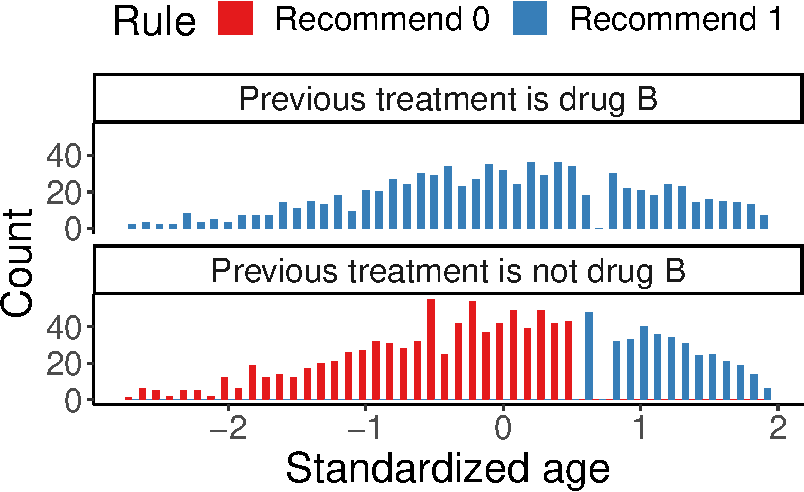
\includegraphics{chapter_18_files/figure-pdf/itr.list.scatter-1.pdf}

}

\end{figure}

The subgroup-level annualized relapse rate (ARR) can be calculated based
on the listDTR ITR:

\begin{Shaded}
\begin{Highlighting}[]
\NormalTok{df.list3 }\SpecialCharTok{\%\textgreater{}\%}
  \FunctionTok{group\_by}\NormalTok{(trt, d.list) }\SpecialCharTok{\%\textgreater{}\%}
  \FunctionTok{summarise}\NormalTok{(}\AttributeTok{ARR =} \FunctionTok{round}\NormalTok{(}\FunctionTok{sum}\NormalTok{(y) }\SpecialCharTok{/} \FunctionTok{sum}\NormalTok{(years), }\DecValTok{2}\NormalTok{),}
            \AttributeTok{n =} \FunctionTok{n}\NormalTok{(),}
            \StringTok{\textasciigrave{}}\AttributeTok{prop\%}\StringTok{\textasciigrave{}} \OtherTok{=} \FunctionTok{round}\NormalTok{(n }\SpecialCharTok{/} \FunctionTok{nrow}\NormalTok{(df), }\DecValTok{2}\NormalTok{)}\SpecialCharTok{*}\DecValTok{100}\NormalTok{, }\AttributeTok{.groups =} \StringTok{"drop"}\NormalTok{) }\SpecialCharTok{\%\textgreater{}\%}
  \FunctionTok{rename}\NormalTok{(}\StringTok{"listDTR ITR"} \OtherTok{=}\NormalTok{ d.list,}
         \StringTok{"Observed treatment"} \OtherTok{=}\NormalTok{ trt) }\SpecialCharTok{\%\textgreater{}\%}
  \FunctionTok{kable}\NormalTok{() }\SpecialCharTok{\%\textgreater{}\%}
  \FunctionTok{kable\_styling}\NormalTok{(}\AttributeTok{full\_width =}\NormalTok{ F)}
\end{Highlighting}
\end{Shaded}

\begin{table}
\centering
\begin{tabular}{l|l|r|r|r}
\hline
Observed treatment & listDTR ITR & ARR & n & prop\%\\
\hline
drug0 & Recommend 0 & 0.32 & 197 & 10\\
\hline
drug0 & Recommend 1 & 0.31 & 309 & 15\\
\hline
drug1 & Recommend 0 & 0.39 & 615 & 31\\
\hline
drug1 & Recommend 1 & 0.16 & 879 & 44\\
\hline
\end{tabular}
\end{table}

Patients who received drug 0 and were recommended drug 0 by listDTR had
a similar ARR on average than those who received drug 0 but were
recommended drug 1 (0.32 vs 0.31). Patients who received drug 1 and were
recommended drug 1 by listDTR had a much lower ARR on average than those
who received drug 1 but were recommended drug 0 (0.16 vs 0.39).

\hypertarget{score-based-method}{%
\subsubsection{Score-based method}\label{score-based-method}}

Although some PM methods do not have built-in visualization or not as
``white-box'' as some more interpretable methods, there still might be
ways to visualize the ITR. For example, score-based methods (such as
Poisson and contrast regression) produce an estimate of the CATE score
for each patient, and a classification tree can be fitted on these
scores and visualized. Below is a histogram-density plot of the CATE
scores estimated from the Poisson regression and the fitted
classification tree using the estimated CATE scores. We pruned the tree
so it only had three nodes for simplicity. The \texttt{rpart.plot}
package has a built-in visualization function of the \texttt{rpart}
model, \texttt{rpart.plot()}, which is how Figure 1B in the chapter was
generated.

\begin{Shaded}
\begin{Highlighting}[]
\NormalTok{df[}\StringTok{"score.poisson"}\NormalTok{] }\OtherTok{\textless{}{-}}\NormalTok{ modpm}\SpecialCharTok{$}\NormalTok{score.poisson}

\FunctionTok{ggplot}\NormalTok{(df, }\FunctionTok{aes}\NormalTok{(}\AttributeTok{x =}\NormalTok{ score.poisson)) }\SpecialCharTok{+} 
  \FunctionTok{geom\_histogram}\NormalTok{(}\FunctionTok{aes}\NormalTok{(}\AttributeTok{y =}\NormalTok{ ..density..), }\AttributeTok{colour =} \StringTok{"black"}\NormalTok{, }\AttributeTok{fill =} \StringTok{"lightblue"}\NormalTok{) }\SpecialCharTok{+}
  \FunctionTok{geom\_density}\NormalTok{(}\AttributeTok{alpha =}\NormalTok{ .}\DecValTok{2}\NormalTok{, }\AttributeTok{fill =} \StringTok{"white"}\NormalTok{) }\SpecialCharTok{+}
  \FunctionTok{labs}\NormalTok{(}\AttributeTok{x =} \StringTok{"Estimated CATE score from the Poisson regression"}\NormalTok{, }\AttributeTok{y =} \StringTok{"Density"}\NormalTok{) }\SpecialCharTok{+} 
  \FunctionTok{theme\_classic}\NormalTok{()}
\end{Highlighting}
\end{Shaded}

\begin{verbatim}
Warning: The dot-dot notation (`..density..`) was deprecated in ggplot2 3.4.0.
i Please use `after_stat(density)` instead.
\end{verbatim}

\begin{verbatim}
`stat_bin()` using `bins = 30`. Pick better value with `binwidth`.
\end{verbatim}

\begin{figure}[H]

{\centering 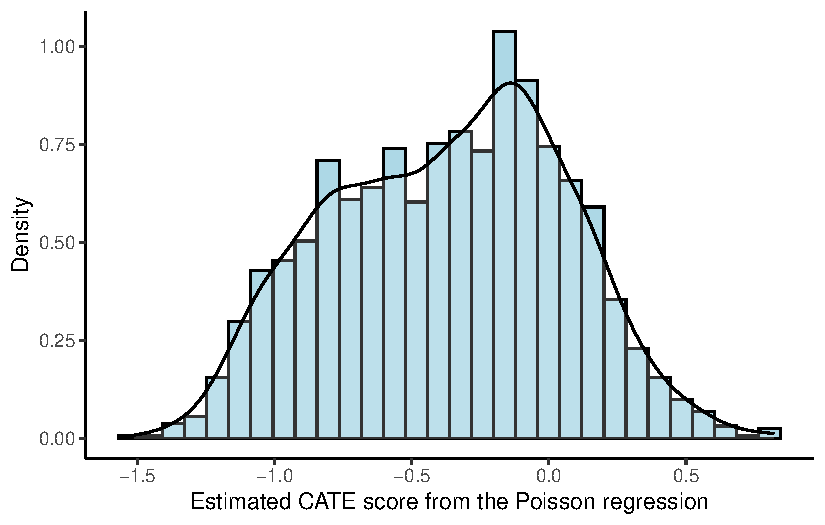
\includegraphics{chapter_18_files/figure-pdf/itr.tree-1.pdf}

}

\end{figure}

\begin{Shaded}
\begin{Highlighting}[]
\NormalTok{modtree }\OtherTok{\textless{}{-}} \FunctionTok{rpart}\NormalTok{(}\FunctionTok{as.formula}\NormalTok{(}\FunctionTok{paste0}\NormalTok{(}\StringTok{"score.poisson \textasciitilde{}"}\NormalTok{, }\FunctionTok{paste0}\NormalTok{(covars, }\AttributeTok{collapse =} \StringTok{"+"}\NormalTok{))),}
                 \AttributeTok{method =} \StringTok{"anova"}\NormalTok{, }\AttributeTok{data =}\NormalTok{ df, }\AttributeTok{control =} \FunctionTok{rpart.control}\NormalTok{(}\AttributeTok{minsplit =} \DecValTok{100}\NormalTok{, }\AttributeTok{cp =} \FloatTok{0.01}\NormalTok{)) }\CommentTok{\# Fit Poisson CATE scores on a classification tree}

\NormalTok{modtree.pr }\OtherTok{\textless{}{-}} \FunctionTok{prune}\NormalTok{(modtree, }\AttributeTok{cp =} \FloatTok{0.09}\NormalTok{) }\CommentTok{\# I ended up choosing a higher cp value to have only 3 subgroups}

\CommentTok{\# print(rpart.rules(modtree.pr, cover = TRUE))}

\DocumentationTok{\#\# Figure 1B}
\FunctionTok{rpart.plot}\NormalTok{(modtree.pr, }\AttributeTok{box.palette =} \StringTok{"RdBu"}\NormalTok{, }\AttributeTok{type =} \DecValTok{5}\NormalTok{, }\AttributeTok{under =} \ConstantTok{TRUE}\NormalTok{, }\AttributeTok{tweak =} \FloatTok{1.2}\NormalTok{, }\AttributeTok{compress =} \ConstantTok{TRUE}\NormalTok{)}
\end{Highlighting}
\end{Shaded}

\begin{figure}[H]

{\centering 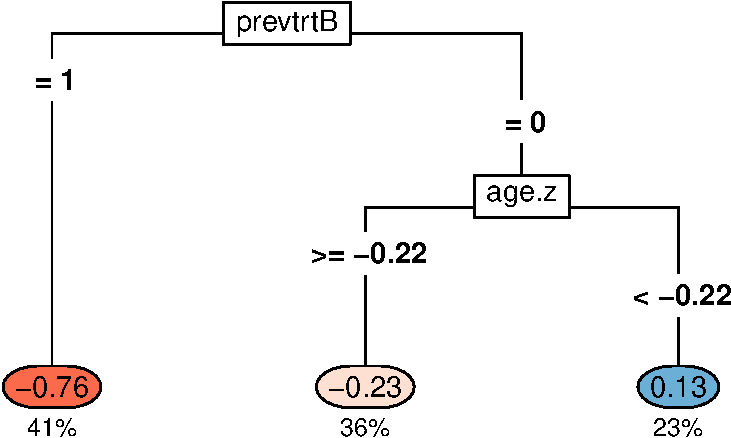
\includegraphics{chapter_18_files/figure-pdf/itr.tree-2.pdf}

}

\end{figure}

The CATE scores are now simplified as a tree classifier. Previous
treatment of drug B and age seemed to be important in determining the
CATE score values, which also showed up in the estimated from the
listDTR method. Patients with previous treatment of drug B had the
lowest CATE score on average (-0.76) and took up 41\% of the samples
(dark orange). Patients whose previous treatment was not drug B and age
was \textgreater= -0.22 standard deviation of the mean also had a
negative CATE score on average (-0.23) and took up 36\% of the samples
(light orange), but not as low as the dark orange group. Negative CATE
scores mean that the number of relapses was expected to be lower for
those recommended drug 1 than those recommended drug 0, so drug 1 was
favored for them. For the blue group, the average CATE score was 0.13,
taking up 23\% of the samples, and they were expected to benefit from
drug 0 based on the Poisson CATE scores.

\hypertarget{itr-accuracy}{%
\subsection{ITR accuracy}\label{itr-accuracy}}

The accuracy of ITR is the proportion of patients whose estimated ITR is
the same as the true optimal ITR. The estimated ITRs have been obtained
from the PM methods but we need to calculate the true optimal ITR. This
is only possible for simulated data where the decision boundary is
known. Based on the data generating mechanism in
\texttt{simcountdata()}, \texttt{Iscore} is a score generated from a
linear combination of baseline covariates where lower scores represented
that drug 1 was better and higher scores represented that drug 0 was
better. We then classified patients in 5 equal-size subgroups based on
the \texttt{Iscore}, where groups 1 and 2 have drug 1 as their true
optimal ITR and groups 3 and 4 have drug 0 as their true optimal ITR.
Group 3 is considered the neutral group, where patients are indifferent
to either drug so we assign the true optimal ITR to be their observed
treatment. Thus, we identify the true optimal ITR for every patient
based on this subgrouping, which was derived from their true score
\texttt{Iscore}. Since we used cross validation in estimating the ITR,
we need to apply the exact same cross validation to the true optimal
ITR. This is achieved by specifying the same randomization seed in the
cross validation loop (see \texttt{seed}).

\begin{Shaded}
\begin{Highlighting}[]
\DocumentationTok{\#\# Create new columns}
\NormalTok{dhats}\SpecialCharTok{$}\NormalTok{d }\OtherTok{\textless{}{-}} \FunctionTok{rep}\NormalTok{(}\ConstantTok{NA}\NormalTok{, }\FunctionTok{nrow}\NormalTok{(dhats)) }\CommentTok{\# true d}

\CommentTok{\# Identify the true optimal treatment}
\CommentTok{\# See simcountdata() in the function script to learn more about Iscore}
\NormalTok{sim }\OtherTok{\textless{}{-}}\NormalTok{ df }\SpecialCharTok{\%\textgreater{}\%}
  \FunctionTok{mutate}\NormalTok{(}\AttributeTok{trueT =} \FunctionTok{ifelse}\NormalTok{(}\FunctionTok{as.numeric}\NormalTok{(Iscore) }\SpecialCharTok{\textless{}} \DecValTok{3}\NormalTok{, }\DecValTok{1}\NormalTok{, }\DecValTok{0}\NormalTok{),}
         \AttributeTok{trueT =} \FunctionTok{ifelse}\NormalTok{(Iscore }\SpecialCharTok{==} \DecValTok{3}\NormalTok{, drug1, trueT)) }\CommentTok{\# neutral group}

\CommentTok{\# Format data}
\NormalTok{input }\OtherTok{\textless{}{-}} \FunctionTok{data.frame}\NormalTok{(}\AttributeTok{y =}\NormalTok{ sim}\SpecialCharTok{$}\NormalTok{y, }\AttributeTok{trt =}\NormalTok{ sim}\SpecialCharTok{$}\NormalTok{drug1, }\AttributeTok{time =} \FunctionTok{log}\NormalTok{(sim}\SpecialCharTok{$}\NormalTok{years), sim[covars])}

\CommentTok{\# Cross validation loop}
\ControlFlowTok{for}\NormalTok{(i }\ControlFlowTok{in} \FunctionTok{unique}\NormalTok{(dhats}\SpecialCharTok{$}\NormalTok{cv.i)) \{}
\NormalTok{  seed }\OtherTok{\textless{}{-}}\NormalTok{ base.seed}\SpecialCharTok{*}\DecValTok{100} \SpecialCharTok{+} \FunctionTok{as.numeric}\NormalTok{(}\FunctionTok{str\_extract}\NormalTok{(i, }\StringTok{"[0{-}9]+"}\NormalTok{))}
  \FunctionTok{set.seed}\NormalTok{(seed)}

  \CommentTok{\# Create CV folds}
\NormalTok{  folds }\OtherTok{\textless{}{-}} \FunctionTok{createFolds}\NormalTok{(input}\SpecialCharTok{$}\NormalTok{trt, }\AttributeTok{k =}\NormalTok{ n.fold, }\AttributeTok{list =} \ConstantTok{TRUE}\NormalTok{) }\CommentTok{\# Stratified CV, follow the same as the simmain.R where folds were created on input$trt instead of sim$trt}

  \ControlFlowTok{for}\NormalTok{ (fold.i }\ControlFlowTok{in} \DecValTok{1}\SpecialCharTok{:}\NormalTok{n.fold)\{}
\NormalTok{    testdata }\OtherTok{\textless{}{-}}\NormalTok{ sim[folds[[fold.i]],]}
    \CommentTok{\# number of methods which succeeded for the given fold/batch. The "is.na(dhat) == FALSE" is to remove methods that didn\textquotesingle{}t produce results for that fold/batch}
\NormalTok{    nr }\OtherTok{\textless{}{-}} \FunctionTok{nrow}\NormalTok{(dhats }\SpecialCharTok{\%\textgreater{}\%} \FunctionTok{filter}\NormalTok{(fold }\SpecialCharTok{==} \FunctionTok{paste0}\NormalTok{(}\StringTok{"fold"}\NormalTok{, fold.i), cv.i }\SpecialCharTok{==}\NormalTok{ i, }\FunctionTok{is.na}\NormalTok{(dhat) }\SpecialCharTok{==} \ConstantTok{FALSE}\NormalTok{))}
\NormalTok{    dhats}\SpecialCharTok{$}\NormalTok{d[}\FunctionTok{which}\NormalTok{(dhats}\SpecialCharTok{$}\NormalTok{fold }\SpecialCharTok{==} \FunctionTok{paste0}\NormalTok{(}\StringTok{"fold"}\NormalTok{, fold.i) }\SpecialCharTok{\&}\NormalTok{ dhats}\SpecialCharTok{$}\NormalTok{cv.i }\SpecialCharTok{==}\NormalTok{ i }\SpecialCharTok{\&} \FunctionTok{is.na}\NormalTok{(dhats}\SpecialCharTok{$}\NormalTok{dhat) }\SpecialCharTok{==} \ConstantTok{FALSE}\NormalTok{)] }\OtherTok{\textless{}{-}} \FunctionTok{rep}\NormalTok{(testdata}\SpecialCharTok{$}\NormalTok{trueT, nr}\SpecialCharTok{/}\FunctionTok{nrow}\NormalTok{(testdata))}
    \FunctionTok{stopifnot}\NormalTok{(nr }\SpecialCharTok{\%\%} \FunctionTok{nrow}\NormalTok{(testdata) }\SpecialCharTok{==} \DecValTok{0}\NormalTok{)}
\NormalTok{  \}}
\NormalTok{\} }\CommentTok{\# end of all cv iterations}
\end{Highlighting}
\end{Shaded}

Once we identified the true optimal ITR (\(d^{opt}\)), we can calculate
the accuracy in each validation fold for each PM method
(\(\hat{d}_{pm}\)). Mathematically, accuracy can be expressed as
\[Accuracy_{pm}(\boldsymbol{x}^{val}) = \frac{1}{n^{val}}\sum_{i = 1}^{n^{val}} I\big(\hat{d}_{pm}(\boldsymbol{x}_i^{val}) == d^{opt}(\boldsymbol{x}_i^{val})\big),\]
where \(n^{val}\) is the sample size in the validation fold,
\(\boldsymbol{x}_i^{val}\) is the baseline characteristics of the
\(i\)th patient in the validation fold, and \(pm\) stands for one PM
method.

Below is how Figure 2 in the chapter was generated. It summarized the
accuracy across all validation folds as a box plot so we can also learn
the variability of accuracy across folds.

\begin{Shaded}
\begin{Highlighting}[]
\DocumentationTok{\#\#\#\#\# Accuracy \#\#\#\#\#}
\DocumentationTok{\#\# Calculate \% accuracy for each iteration \& summary statistics}
\NormalTok{dhats.accuracy }\OtherTok{\textless{}{-}}\NormalTok{ dhats }\SpecialCharTok{\%\textgreater{}\%}
  \FunctionTok{group\_by}\NormalTok{(method, cv.i, fold) }\SpecialCharTok{\%\textgreater{}\%}
  \FunctionTok{summarise}\NormalTok{(}\AttributeTok{accuracy =} \FunctionTok{sum}\NormalTok{(dhat }\SpecialCharTok{==}\NormalTok{ d)}\SpecialCharTok{/}\FunctionTok{n}\NormalTok{(), }\AttributeTok{.groups =} \StringTok{"drop"}\NormalTok{) }\SpecialCharTok{\%\textgreater{}\%}
\NormalTok{  ungroup}

\DocumentationTok{\#\# Make the accuracy plot, Figure 2}
\NormalTok{dhats.accuracy }\SpecialCharTok{\%\textgreater{}\%}
  \FunctionTok{ggplot}\NormalTok{(}\FunctionTok{aes}\NormalTok{(}\AttributeTok{x =}\NormalTok{ method, }\AttributeTok{y =}\NormalTok{ accuracy)) }\SpecialCharTok{+}
  \FunctionTok{geom\_boxplot}\NormalTok{() }\SpecialCharTok{+}
  \FunctionTok{geom\_hline}\NormalTok{(}\AttributeTok{yintercept =} \DecValTok{1}\NormalTok{, }\AttributeTok{linetype =} \DecValTok{2}\NormalTok{, }\AttributeTok{linewidth =} \DecValTok{1}\NormalTok{, }\AttributeTok{color =} \StringTok{"gray"}\NormalTok{) }\SpecialCharTok{+}
  \FunctionTok{geom\_hline}\NormalTok{(}\AttributeTok{yintercept =} \FloatTok{0.5}\NormalTok{, }\AttributeTok{linetype =} \DecValTok{2}\NormalTok{, }\AttributeTok{linewidth =} \DecValTok{1}\NormalTok{, }\AttributeTok{color =} \StringTok{"gray"}\NormalTok{) }\SpecialCharTok{+}
  \FunctionTok{theme\_classic}\NormalTok{() }\SpecialCharTok{+}
  \FunctionTok{labs}\NormalTok{(}\AttributeTok{x =} \StringTok{"Method"}\NormalTok{, }\AttributeTok{y =} \StringTok{"Accuracy"}\NormalTok{) }\SpecialCharTok{+}
  \FunctionTok{theme}\NormalTok{(}\AttributeTok{axis.text =} \FunctionTok{element\_text}\NormalTok{(}\AttributeTok{size =} \DecValTok{15}\NormalTok{),}
        \AttributeTok{axis.title.y =} \FunctionTok{element\_text}\NormalTok{(}\AttributeTok{size =} \DecValTok{15}\NormalTok{),}
        \AttributeTok{axis.title.x =} \FunctionTok{element\_text}\NormalTok{(}\AttributeTok{size =} \DecValTok{15}\NormalTok{),}
        \AttributeTok{axis.text.x =} \FunctionTok{element\_text}\NormalTok{(}\AttributeTok{angle =} \DecValTok{0}\NormalTok{, }\AttributeTok{size =} \DecValTok{15}\NormalTok{),}
        \AttributeTok{strip.text.x =} \FunctionTok{element\_text}\NormalTok{(}\AttributeTok{size =} \DecValTok{15}\NormalTok{))}
\end{Highlighting}
\end{Shaded}

\begin{figure}[H]

{\centering 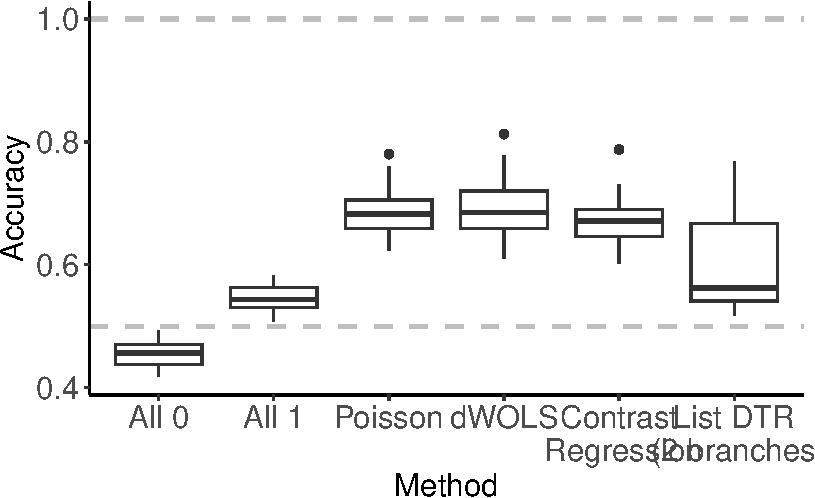
\includegraphics{chapter_18_files/figure-pdf/accuracy-1.pdf}

}

\end{figure}

\hypertarget{itr-agreement}{%
\subsection{ITR agreement}\label{itr-agreement}}

When we do not know the true data generating mechanism, e.g., real-world
data, we cannot compare the estimated ITR with the true optimal ITR.
However, we can compare the estimated ITR with another estimated ITR,
and this is called agreement. Agreement is the proportion of patients
whose estimated ITR of a method is the same as the estimated ITR of
another method. Thus, agreement is between two methods. Mathematically,
\[Agreement_{1, 2}(\boldsymbol{x}^{val}) = \frac{1}{n^{val}} \sum_{i = 1}^{n^{val}} I\big( \hat{d}_{1}(\boldsymbol{x}^{val}) == \hat{d}_{2} (\boldsymbol{x}^{val}) \big), \]
where \(n^{val}\) is the sample size in the validation fold,
\(\boldsymbol{x}_i^{val}\) is the baseline characteristics of the
\(i\)th patient in the validation fold, and \(1, 2\) stands for method 1
and method 2.

\begin{Shaded}
\begin{Highlighting}[]
\DocumentationTok{\#\#\#\#\# Agreement \#\#\#\#\#}
\NormalTok{dhats.concat }\OtherTok{\textless{}{-}}\NormalTok{ dhats }\SpecialCharTok{\%\textgreater{}\%}
  \FunctionTok{arrange}\NormalTok{(cv.i, fold, method) }\SpecialCharTok{\%\textgreater{}\%}
  \FunctionTok{mutate}\NormalTok{(}\AttributeTok{iteration.fold =}\NormalTok{ (}\FunctionTok{as.numeric}\NormalTok{(}\FunctionTok{str\_extract}\NormalTok{(cv.i, }\StringTok{"[0{-}9]+"}\NormalTok{)) }\SpecialCharTok{{-}} \DecValTok{1}\NormalTok{) }\SpecialCharTok{*} \DecValTok{10} \SpecialCharTok{+} \FunctionTok{as.numeric}\NormalTok{(}\FunctionTok{str\_extract}\NormalTok{(fold, }\StringTok{"[0{-}9]+"}\NormalTok{))) }\SpecialCharTok{\%\textgreater{}\%} 
\NormalTok{  dplyr}\SpecialCharTok{::}\FunctionTok{select}\NormalTok{(method, iteration.fold, dhat) }\SpecialCharTok{\%\textgreater{}\%}
  \FunctionTok{group\_by}\NormalTok{(method, iteration.fold) }\SpecialCharTok{\%\textgreater{}\%}
  \FunctionTok{mutate}\NormalTok{(}\AttributeTok{i =} \DecValTok{1}\SpecialCharTok{:}\FunctionTok{n}\NormalTok{()) }\SpecialCharTok{\%\textgreater{}\%}  
\NormalTok{  ungroup}

\NormalTok{m }\OtherTok{\textless{}{-}} \FunctionTok{length}\NormalTok{(method.vec)}
\NormalTok{dhats.agreement }\OtherTok{\textless{}{-}} \FunctionTok{matrix}\NormalTok{(}\AttributeTok{nrow =}\NormalTok{ m, }\AttributeTok{ncol =}\NormalTok{ m)}
\FunctionTok{colnames}\NormalTok{(dhats.agreement) }\OtherTok{\textless{}{-}}\NormalTok{ method.vec}
\FunctionTok{rownames}\NormalTok{(dhats.agreement) }\OtherTok{\textless{}{-}}\NormalTok{ method.vec}

\ControlFlowTok{for}\NormalTok{(k }\ControlFlowTok{in} \FunctionTok{seq\_len}\NormalTok{(m))\{}
  \ControlFlowTok{for}\NormalTok{(j }\ControlFlowTok{in} \FunctionTok{seq}\NormalTok{(k, m))\{}
\NormalTok{    data.k }\OtherTok{\textless{}{-}}\NormalTok{ dhats.concat }\SpecialCharTok{\%\textgreater{}\%} \FunctionTok{filter}\NormalTok{(method }\SpecialCharTok{==}\NormalTok{ method.vec[k])}
\NormalTok{    data.j }\OtherTok{\textless{}{-}}\NormalTok{ dhats.concat }\SpecialCharTok{\%\textgreater{}\%} \FunctionTok{filter}\NormalTok{(method }\SpecialCharTok{==}\NormalTok{ method.vec[j])}
\NormalTok{    data.jk }\OtherTok{\textless{}{-}}\NormalTok{ data.k }\SpecialCharTok{\%\textgreater{}\%} \FunctionTok{full\_join}\NormalTok{(data.j, }\AttributeTok{by =} \FunctionTok{c}\NormalTok{(}\StringTok{"iteration.fold"}\NormalTok{, }\StringTok{"i"}\NormalTok{))}
\NormalTok{    dhats.agreement[k, j] }\OtherTok{\textless{}{-}}\NormalTok{ dhats.agreement[j, k] }\OtherTok{\textless{}{-}} \FunctionTok{sum}\NormalTok{(data.jk}\SpecialCharTok{$}\NormalTok{dhat.x }\SpecialCharTok{==}\NormalTok{ data.jk}\SpecialCharTok{$}\NormalTok{dhat.y, }\AttributeTok{na.rm =}\NormalTok{ T) }\SpecialCharTok{/} \FunctionTok{sum}\NormalTok{(}\FunctionTok{is.na}\NormalTok{(data.jk}\SpecialCharTok{$}\NormalTok{dhat.x) }\SpecialCharTok{==} \ConstantTok{FALSE} \SpecialCharTok{\&} \FunctionTok{is.na}\NormalTok{(data.jk}\SpecialCharTok{$}\NormalTok{dhat.y) }\SpecialCharTok{==} \ConstantTok{FALSE}\NormalTok{)}
\NormalTok{  \}}
\NormalTok{\}}

\CommentTok{\# Make the agreement plot, Figure 3}
\FunctionTok{corrplot}\NormalTok{(dhats.agreement, }\AttributeTok{method =} \StringTok{"color"}\NormalTok{,  }\AttributeTok{type =} \StringTok{"lower"}\NormalTok{,}
         \AttributeTok{addCoef.col =} \StringTok{"orange"}\NormalTok{, }\AttributeTok{number.cex =} \FloatTok{1.5}\NormalTok{,}
         \AttributeTok{tl.cex =} \FloatTok{1.2}\NormalTok{, }\AttributeTok{cl.cex =} \FloatTok{1.2}\NormalTok{, }\AttributeTok{tl.col =} \StringTok{"black"}\NormalTok{, }\AttributeTok{tl.srt =} \DecValTok{0}\NormalTok{, }\AttributeTok{tl.offset =} \FloatTok{1.5}\NormalTok{)}
\end{Highlighting}
\end{Shaded}

\begin{figure}[H]

{\centering 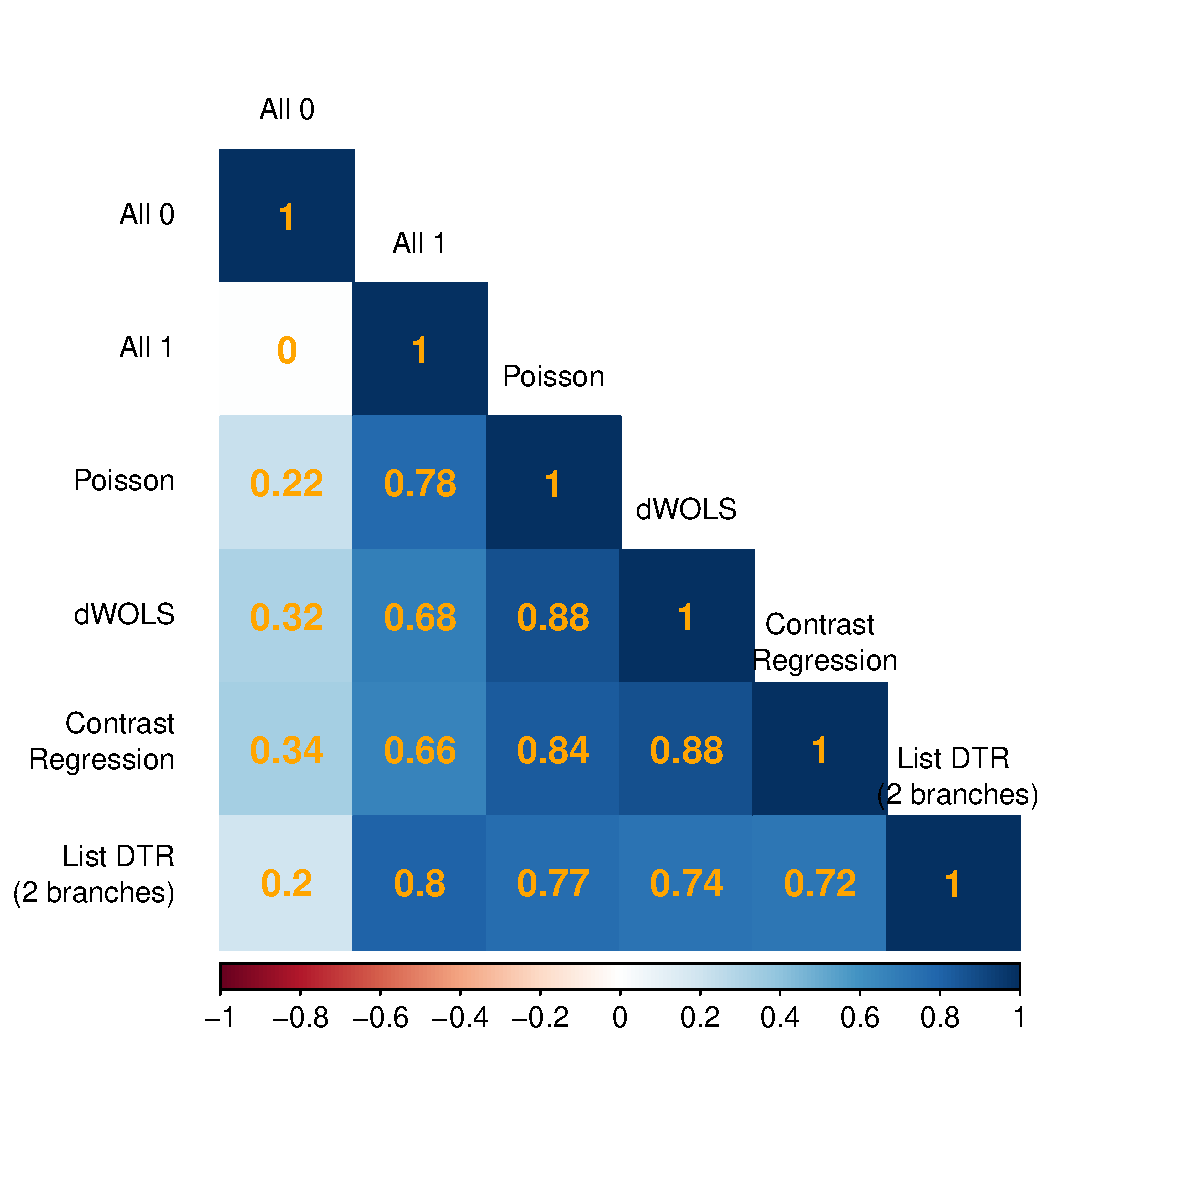
\includegraphics{chapter_18_files/figure-pdf/agreement-1.pdf}

}

\end{figure}

We used the \texttt{corrplot} package to generate Figure 3 in the
chapter but agreement can be visualized in other creative ways that you
prefer.

\hypertarget{patient-well-being}{%
\section{Patient well-being}\label{patient-well-being}}

Patient well-being is evaluated via the value function, which is defined
as the expected outcome had they followed the specified ITR. Like a
fortune teller's crystal ball, this metric tells us how well the
patients would do on average under each ITR. We can then compare across
different ITRs and identify an optimal ITR. Cross validation is
necessary here to mitigate over-fitting, and we visualized the value
function results as error bar plots. The mean and standard deviation of
the value functions have been preprocessed previously. We use
\texttt{ggplot()} to generate the error bar plots. Figure 4A is the
original value function estimates, and Figure 4B is the standardized
value ratio estimates, which convert value functions to a ratio where 1
is always more desirable.

\begin{Shaded}
\begin{Highlighting}[]
\DocumentationTok{\#\#\#\#\# Errorbar plot \#\#\#\#\#}
\CommentTok{\# Figure 4A}
\NormalTok{p4a }\OtherTok{\textless{}{-}}\NormalTok{ vhats.dhat }\SpecialCharTok{\%\textgreater{}\%}
  \FunctionTok{ggplot}\NormalTok{(}\FunctionTok{aes}\NormalTok{(}\AttributeTok{x =}\NormalTok{ method, }\AttributeTok{y =}\NormalTok{ meanV)) }\SpecialCharTok{+}
  \FunctionTok{geom\_point}\NormalTok{(}\AttributeTok{size =} \DecValTok{8}\NormalTok{, }\AttributeTok{shape =} \DecValTok{16}\NormalTok{, }\AttributeTok{color =} \StringTok{"navy"}\NormalTok{) }\SpecialCharTok{+}
  \FunctionTok{geom\_errorbar}\NormalTok{(}\FunctionTok{aes}\NormalTok{(}\AttributeTok{ymin =}\NormalTok{ meanV }\SpecialCharTok{{-}}\NormalTok{ sdV, }\AttributeTok{ymax =}\NormalTok{ meanV }\SpecialCharTok{+}\NormalTok{ sdV), }\AttributeTok{width =} \FloatTok{0.3}\NormalTok{, }\AttributeTok{size =} \DecValTok{2}\NormalTok{, }\AttributeTok{position =} \FunctionTok{position\_dodge}\NormalTok{(}\FloatTok{0.9}\NormalTok{), }\AttributeTok{color =} \StringTok{"navy"}\NormalTok{) }\SpecialCharTok{+}
  \FunctionTok{theme\_classic}\NormalTok{() }\SpecialCharTok{+} \FunctionTok{xlab}\NormalTok{(}\StringTok{""}\NormalTok{) }\SpecialCharTok{+} \FunctionTok{ylab}\NormalTok{(}\StringTok{"Cross{-}validated value (mean +{-} SD)"}\NormalTok{) }\SpecialCharTok{+}
  \FunctionTok{theme}\NormalTok{(}\AttributeTok{axis.text =} \FunctionTok{element\_text}\NormalTok{(}\AttributeTok{size =} \DecValTok{15}\NormalTok{), }\AttributeTok{axis.title.y =} \FunctionTok{element\_text}\NormalTok{(}\AttributeTok{size =} \DecValTok{15}\NormalTok{)) }\SpecialCharTok{+}
  \FunctionTok{geom\_hline}\NormalTok{(}\AttributeTok{yintercept =}\NormalTok{ vhats.dhat}\SpecialCharTok{$}\NormalTok{meanV[}\FunctionTok{which}\NormalTok{(vhats.dhat}\SpecialCharTok{$}\NormalTok{method }\SpecialCharTok{==} \StringTok{"All 1"}\NormalTok{)], }\AttributeTok{linetype =} \DecValTok{2}\NormalTok{, }\AttributeTok{size =} \FloatTok{1.5}\NormalTok{, }\AttributeTok{color =} \StringTok{"gray"}\NormalTok{)}
\end{Highlighting}
\end{Shaded}

\begin{verbatim}
Warning: Using `size` aesthetic for lines was deprecated in ggplot2 3.4.0.
i Please use `linewidth` instead.
\end{verbatim}

\begin{Shaded}
\begin{Highlighting}[]
\DocumentationTok{\#\#\#\#\# Value ratio \#\#\#\#\#}
\CommentTok{\# Figure 4B}
\NormalTok{p4b }\OtherTok{\textless{}{-}}\NormalTok{ vhats.dhat }\SpecialCharTok{\%\textgreater{}\%}
\NormalTok{  dplyr}\SpecialCharTok{::}\FunctionTok{select}\NormalTok{(method, }\FunctionTok{contains}\NormalTok{(}\StringTok{"VR"}\NormalTok{), n.nonnaU) }\SpecialCharTok{\%\textgreater{}\%}
  \FunctionTok{ggplot}\NormalTok{(}\FunctionTok{aes}\NormalTok{(}\AttributeTok{x =}\NormalTok{ method, }\AttributeTok{y =}\NormalTok{ meanVR)) }\SpecialCharTok{+}
  \FunctionTok{geom\_point}\NormalTok{(}\AttributeTok{size =} \DecValTok{8}\NormalTok{, }\AttributeTok{color =} \StringTok{"navy"}\NormalTok{) }\SpecialCharTok{+}
  \FunctionTok{geom\_errorbar}\NormalTok{(}\FunctionTok{aes}\NormalTok{(}\AttributeTok{ymin =}\NormalTok{ meanVR }\SpecialCharTok{{-}}\NormalTok{ sdVR, }\AttributeTok{ymax =}\NormalTok{ meanVR }\SpecialCharTok{+}\NormalTok{ sdVR), }\AttributeTok{width =} \FloatTok{0.3}\NormalTok{, }\AttributeTok{size =} \DecValTok{2}\NormalTok{, }\AttributeTok{position =} \FunctionTok{position\_dodge}\NormalTok{(}\FloatTok{0.9}\NormalTok{), }\AttributeTok{color =} \StringTok{"navy"}\NormalTok{) }\SpecialCharTok{+}
  \FunctionTok{geom\_hline}\NormalTok{(}\AttributeTok{yintercept =} \DecValTok{1}\NormalTok{, }\AttributeTok{color =} \StringTok{"gray"}\NormalTok{, }\AttributeTok{linetype =} \DecValTok{2}\NormalTok{, }\AttributeTok{size =} \DecValTok{1}\NormalTok{) }\SpecialCharTok{+}
  \FunctionTok{geom\_hline}\NormalTok{(}\AttributeTok{yintercept =} \DecValTok{0}\NormalTok{, }\AttributeTok{color =} \StringTok{"gray"}\NormalTok{, }\AttributeTok{linetype =} \DecValTok{2}\NormalTok{, }\AttributeTok{size =} \DecValTok{1}\NormalTok{) }\SpecialCharTok{+}
  \FunctionTok{scale\_y\_continuous}\NormalTok{(}\AttributeTok{breaks =} \FunctionTok{seq}\NormalTok{(}\DecValTok{0}\NormalTok{, }\DecValTok{1}\NormalTok{, }\AttributeTok{length =} \DecValTok{6}\NormalTok{)) }\SpecialCharTok{+}
  \FunctionTok{theme\_classic}\NormalTok{() }\SpecialCharTok{+}
  \FunctionTok{labs}\NormalTok{(}\AttributeTok{x =} \StringTok{""}\NormalTok{, }\AttributeTok{y =} \StringTok{"Value ratio of cross{-}validated estimated decision rule (mean +{-} SD)"}\NormalTok{) }\SpecialCharTok{+}
  \FunctionTok{theme}\NormalTok{(}\AttributeTok{axis.text =} \FunctionTok{element\_text}\NormalTok{(}\AttributeTok{size =} \DecValTok{13}\NormalTok{),}
        \AttributeTok{axis.title.y =} \FunctionTok{element\_text}\NormalTok{(}\AttributeTok{size =} \DecValTok{15}\NormalTok{),}
        \AttributeTok{axis.title.x =} \FunctionTok{element\_text}\NormalTok{(}\AttributeTok{size =} \DecValTok{15}\NormalTok{),}
        \AttributeTok{axis.text.x =} \FunctionTok{element\_text}\NormalTok{(}\AttributeTok{size =} \DecValTok{15}\NormalTok{),}
        \AttributeTok{strip.text.x =} \FunctionTok{element\_text}\NormalTok{(}\AttributeTok{size =} \DecValTok{12}\NormalTok{))}

\CommentTok{\# Figure 4}
\FunctionTok{ggarrange}\NormalTok{(p4a, p4b, }\AttributeTok{ncol =} \DecValTok{2}\NormalTok{, }\AttributeTok{nrow =} \DecValTok{1}\NormalTok{, }\AttributeTok{labels =} \FunctionTok{c}\NormalTok{(}\StringTok{"A"}\NormalTok{, }\StringTok{"B"}\NormalTok{))}
\end{Highlighting}
\end{Shaded}

\begin{figure}[H]

{\centering 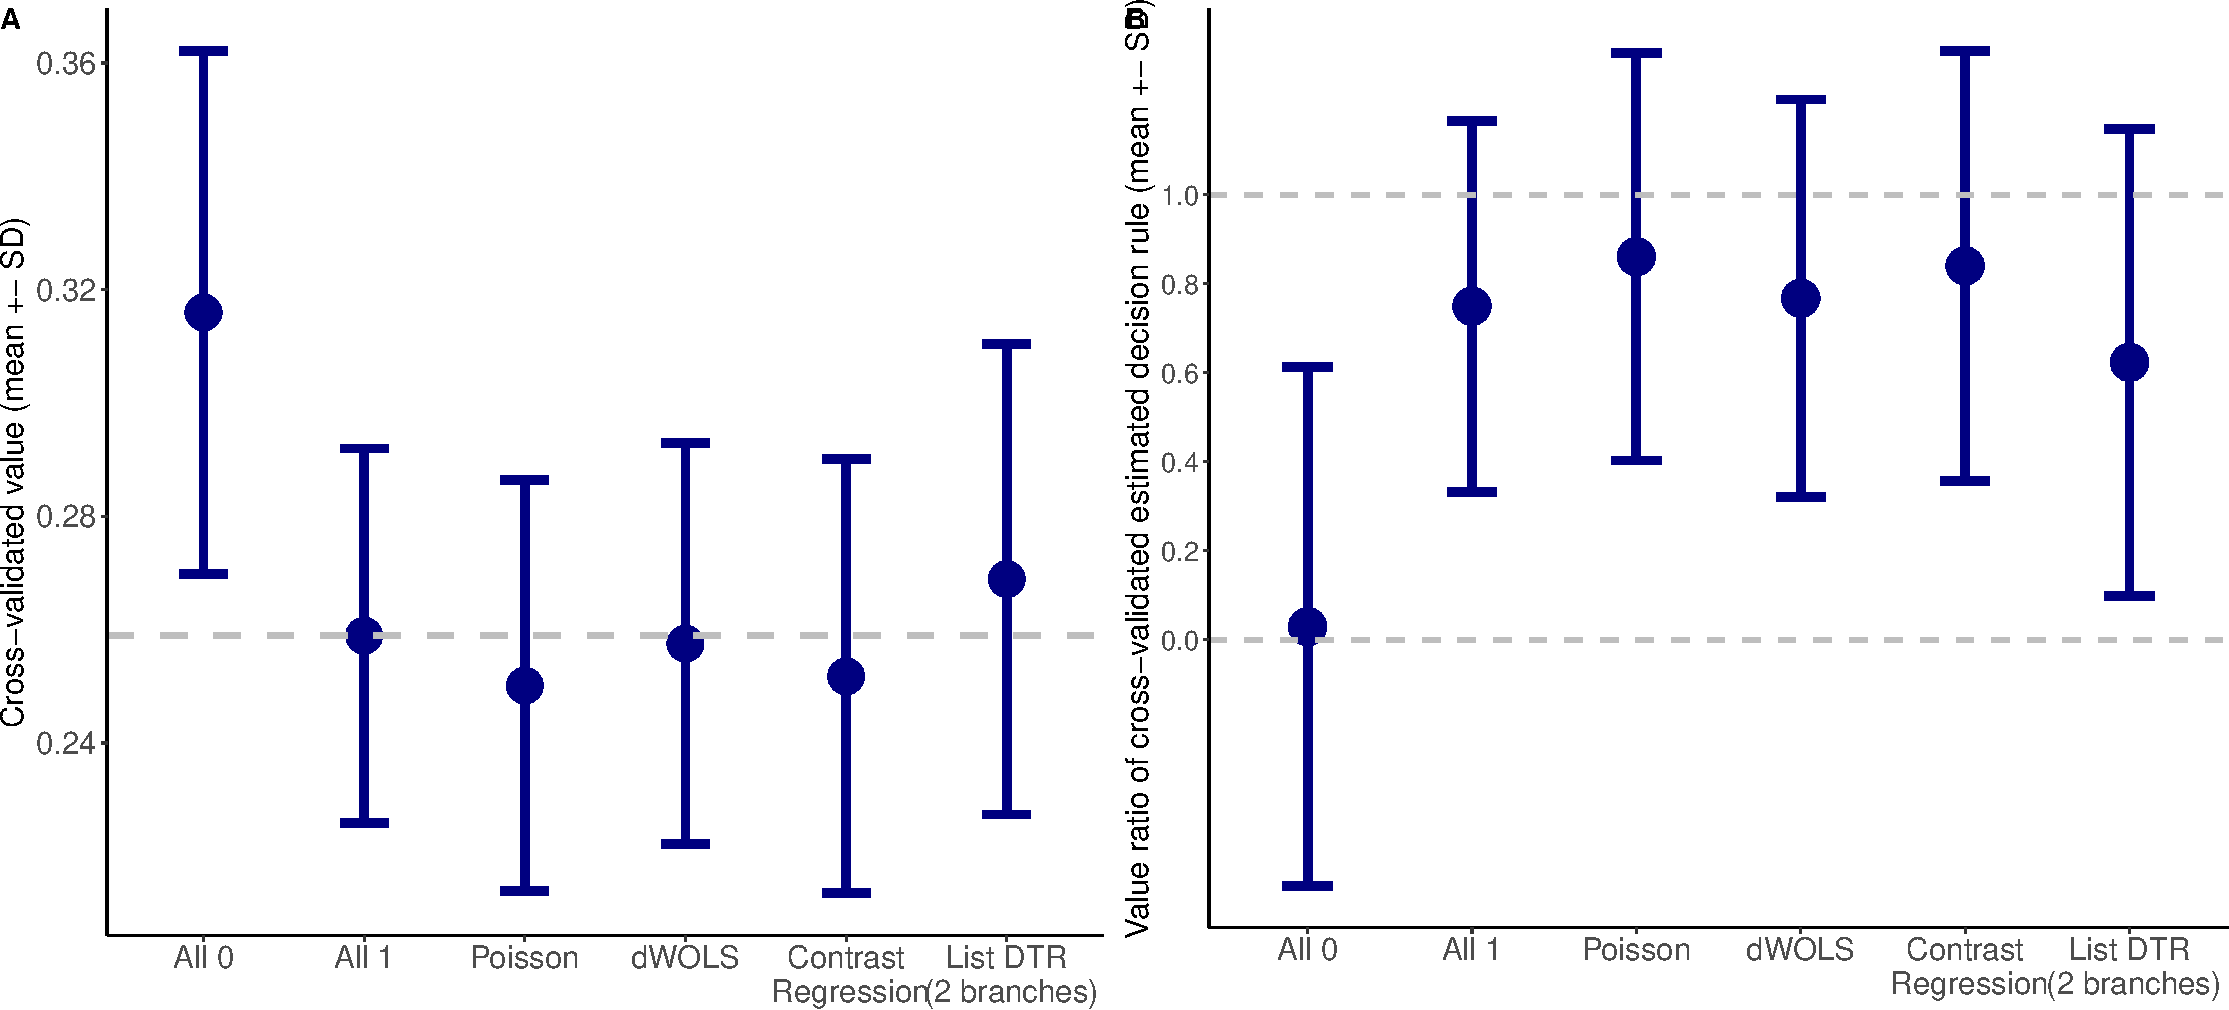
\includegraphics{chapter_18_files/figure-pdf/value-1.pdf}

}

\end{figure}

\hypertarget{responder-diagnostics}{%
\section{Responder diagnostics}\label{responder-diagnostics}}

\hypertarget{validation}{%
\subsection{Validation}\label{validation}}

The package we used for the two score-based methods (Poisson and
contrast regression), \texttt{PrecMed}, has built-in visualization tools
to diagnose the results: validation box plots \texttt{boxplot()},
validation curves \texttt{plot()}, and area between curves (ABC)
statistics \texttt{abc()}.

\begin{Shaded}
\begin{Highlighting}[]
\DocumentationTok{\#\#\#\#\# Validation of ITR scores \#\#\#\#\#}
\CommentTok{\# Figure 5A}
\NormalTok{p5a }\OtherTok{\textless{}{-}} \FunctionTok{boxplot}\NormalTok{(modcv, }\AttributeTok{ylab =} \StringTok{"Rate ratio between T=1 and T=0 in each subgroup"}\NormalTok{)}
\CommentTok{\# Figure 5B}
\NormalTok{p5b }\OtherTok{\textless{}{-}} \FunctionTok{plot}\NormalTok{(modcv, }\AttributeTok{ylab =} \StringTok{"Rate ratio between T=1 and T=0 in each subgroup"}\NormalTok{)}

\CommentTok{\# Figure 5}
\FunctionTok{ggarrange}\NormalTok{(p5a, p5b, }\AttributeTok{ncol =} \DecValTok{1}\NormalTok{, }\AttributeTok{nrow =} \DecValTok{2}\NormalTok{, }\AttributeTok{labels =} \FunctionTok{c}\NormalTok{(}\StringTok{"A"}\NormalTok{, }\StringTok{"B"}\NormalTok{))}
\end{Highlighting}
\end{Shaded}

\begin{figure}[H]

{\centering 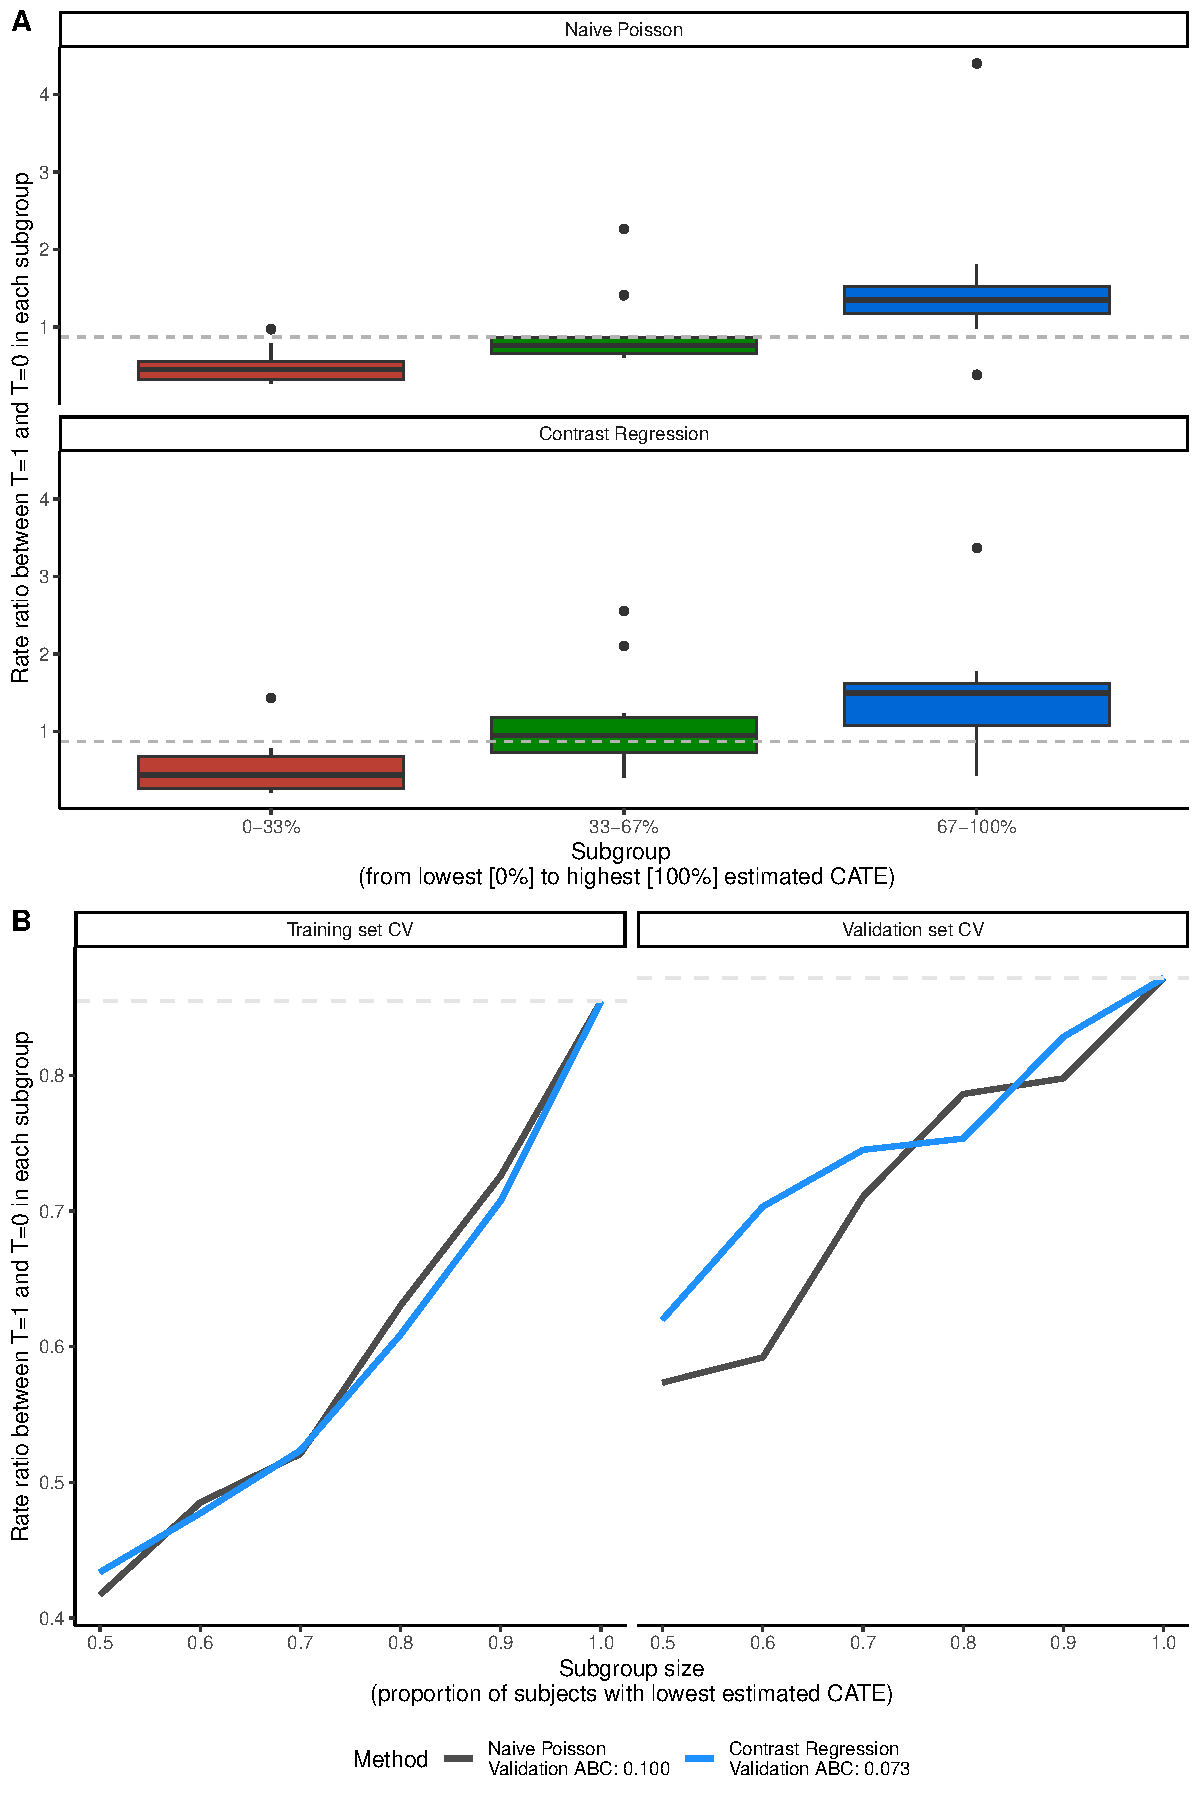
\includegraphics{chapter_18_files/figure-pdf/validation-1.pdf}

}

\end{figure}

The \texttt{PrecMed} package has more PM methods implemented other than
Poisson and contrast regression that you can try, such as negative
binomial and two regressions. See its documentation for more details.

\hypertarget{univariate-comparision-of-patient-characteristics}{%
\subsection{Univariate comparision of patient
characteristics}\label{univariate-comparision-of-patient-characteristics}}

The 60/40 cutoff was used in the chapter to split patients into ``high
responders'' and ``standard responders''. The function
\texttt{CreateTableOne()} in the \texttt{tableone} package was used to
generate a table comparing side-by-side the baseline characteristics
between the two responder groups.

\begin{Shaded}
\begin{Highlighting}[]
\DocumentationTok{\#\#\#\#\# Side{-}by{-}side baseline characteristic comparison between responder subgroups \#\#\#\#\#}
\NormalTok{cutoff }\OtherTok{\textless{}{-}} \FunctionTok{quantile}\NormalTok{(modpm}\SpecialCharTok{$}\NormalTok{score.poisson, }\FloatTok{0.6}\NormalTok{) }\CommentTok{\# 60/40 high vs standard responder split}
\NormalTok{df[}\StringTok{"responder to T=1"}\NormalTok{] }\OtherTok{\textless{}{-}} \FunctionTok{ifelse}\NormalTok{(modpm}\SpecialCharTok{$}\NormalTok{score.poisson }\SpecialCharTok{\textless{}}\NormalTok{ cutoff, }\StringTok{"High"}\NormalTok{, }\StringTok{"Standard"}\NormalTok{)}
\NormalTok{df[}\StringTok{"age.z"}\NormalTok{] }\OtherTok{\textless{}{-}} \FunctionTok{as.numeric}\NormalTok{(df}\SpecialCharTok{$}\NormalTok{age.z)}
\NormalTok{df[}\StringTok{"previous\_cost.z"}\NormalTok{] }\OtherTok{\textless{}{-}} \FunctionTok{as.numeric}\NormalTok{(df}\SpecialCharTok{$}\NormalTok{previous\_cost.z)}

\NormalTok{labs }\OtherTok{\textless{}{-}} \FunctionTok{list}\NormalTok{(}\StringTok{"age.z"} \OtherTok{=} \StringTok{"Standardized baseline age"}\NormalTok{, }\StringTok{"female"} \OtherTok{=} \StringTok{"Female"}\NormalTok{,}
             \StringTok{"prevtrtB"} \OtherTok{=} \StringTok{"Previous treatment drug B"}\NormalTok{, }\StringTok{"prevtrtC"} \OtherTok{=} \StringTok{"Previous treatment drug C"}\NormalTok{,}
             \StringTok{"prevnumsymp1"} \OtherTok{=} \StringTok{"Previous number of symptoms == 1"}\NormalTok{,}
             \StringTok{"prevnumsymp2p"} \OtherTok{=} \StringTok{"Previuos number of symptoms \textgreater{}= 2"}\NormalTok{,}
             \StringTok{"previous\_cost.z"} \OtherTok{=} \StringTok{"Standardized previous medical cost}\SpecialCharTok{\textbackslash{}n}\StringTok{(excluding medication)"}\NormalTok{,}
             \StringTok{"previos\_number\_relapses"} \OtherTok{=} \StringTok{"Previous number of relapses"}\NormalTok{)}

\NormalTok{tab }\OtherTok{\textless{}{-}} \FunctionTok{CreateTableOne}\NormalTok{(}\AttributeTok{vars =}\NormalTok{ covars, }\AttributeTok{strata =} \StringTok{"responder to T=1"}\NormalTok{, }\AttributeTok{data =}\NormalTok{ df, }\AttributeTok{test =}\NormalTok{ F) }\SpecialCharTok{\%\textgreater{}\%} \FunctionTok{print}\NormalTok{(}\AttributeTok{smd =}\NormalTok{ T)}
\end{Highlighting}
\end{Shaded}

\begin{verbatim}
                                      Stratified by responder to T=1
                                       High         Standard     SMD   
  n                                     1200          800              
  age.z (mean (SD))                     0.29 (0.94) -0.44 (0.92)  0.789
  female (mean (SD))                    0.69 (0.46)  0.84 (0.36)  0.384
  prevtrtB (mean (SD))                  0.67 (0.47)  0.02 (0.15)  1.867
  prevtrtC (mean (SD))                  0.02 (0.13)  0.26 (0.44)  0.750
  prevnumsymp1 (mean (SD))              0.32 (0.47)  0.15 (0.35)  0.431
  prevnumsymp2p (mean (SD))             0.05 (0.22)  0.11 (0.31)  0.208
  previous_cost.z (mean (SD))          -0.08 (1.00)  0.12 (0.99)  0.203
  previous_number_relapses (mean (SD))  0.41 (0.64)  0.47 (0.68)  0.104
\end{verbatim}

We can directly present the table or visualize the comparison with
errorbar plots, which is what the chapter presented (Figure 6A). Here we
show both. Tables are helpful if specific numbers are important but
readers would have to perform mental comparison to understand which
value is higher, whereas plots are helpful if you want people to quickly
identify the larger differences and not focus on the specific values of
certain results.

\begin{Shaded}
\begin{Highlighting}[]
\NormalTok{smd }\OtherTok{\textless{}{-}} \FunctionTok{as\_tibble}\NormalTok{(tab, }\AttributeTok{rownames =} \StringTok{"var"}\NormalTok{) }\SpecialCharTok{\%\textgreater{}\%}
  \FunctionTok{rowwise}\NormalTok{() }\SpecialCharTok{\%\textgreater{}\%}
  \FunctionTok{mutate}\NormalTok{(}\AttributeTok{variable =} \FunctionTok{as.factor}\NormalTok{(}\FunctionTok{str\_extract}\NormalTok{(var, }\StringTok{".*(?= }\SpecialCharTok{\textbackslash{}\textbackslash{}}\StringTok{(mean }\SpecialCharTok{\textbackslash{}\textbackslash{}}\StringTok{(SD}\SpecialCharTok{\textbackslash{}\textbackslash{}}\StringTok{)}\SpecialCharTok{\textbackslash{}\textbackslash{}}\StringTok{))"}\NormalTok{))) }\SpecialCharTok{\%\textgreater{}\%}
  \FunctionTok{filter}\NormalTok{(}\SpecialCharTok{!}\FunctionTok{is.na}\NormalTok{(variable)) }\SpecialCharTok{\%\textgreater{}\%}
  \FunctionTok{arrange}\NormalTok{(}\FunctionTok{desc}\NormalTok{(SMD)) }\SpecialCharTok{\%\textgreater{}\%}
  \FunctionTok{mutate}\NormalTok{(}\AttributeTok{smd =} \FunctionTok{paste0}\NormalTok{(}\StringTok{"SMD ="}\NormalTok{, SMD),}
         \AttributeTok{variable =}\NormalTok{ labs[[variable]]) }\SpecialCharTok{\%\textgreater{}\%}
\NormalTok{  dplyr}\SpecialCharTok{::}\FunctionTok{select}\NormalTok{(variable, smd) }\SpecialCharTok{\%\textgreater{}\%}
  \FunctionTok{mutate}\NormalTok{(}\AttributeTok{ID =} \DecValTok{1}\NormalTok{)}

\NormalTok{levels }\OtherTok{\textless{}{-}} \FunctionTok{unique}\NormalTok{(smd}\SpecialCharTok{$}\NormalTok{variable)}

\NormalTok{p6a }\OtherTok{\textless{}{-}}\NormalTok{ df }\SpecialCharTok{\%\textgreater{}\%}
  \FunctionTok{mutate}\NormalTok{(}\AttributeTok{ID =} \DecValTok{1}\SpecialCharTok{:}\FunctionTok{n}\NormalTok{()) }\SpecialCharTok{\%\textgreater{}\%}
\NormalTok{  dplyr}\SpecialCharTok{::}\FunctionTok{select}\NormalTok{(}\FunctionTok{all\_of}\NormalTok{(covars), ID, }\FunctionTok{contains}\NormalTok{(}\StringTok{"responder"}\NormalTok{)) }\SpecialCharTok{\%\textgreater{}\%}
  \FunctionTok{melt}\NormalTok{(}\AttributeTok{id =} \FunctionTok{c}\NormalTok{(}\StringTok{"ID"}\NormalTok{, }\StringTok{"responder to T=1"}\NormalTok{)) }\SpecialCharTok{\%\textgreater{}\%}
  \FunctionTok{rowwise}\NormalTok{() }\SpecialCharTok{\%\textgreater{}\%}
  \FunctionTok{mutate}\NormalTok{(}\AttributeTok{variable =}\NormalTok{ labs[[variable]]) }\SpecialCharTok{\%\textgreater{}\%}
  \FunctionTok{left\_join}\NormalTok{(smd, }\AttributeTok{by =} \FunctionTok{c}\NormalTok{(}\StringTok{"variable"}\NormalTok{, }\StringTok{"ID"}\NormalTok{)) }\SpecialCharTok{\%\textgreater{}\%}
  \FunctionTok{mutate}\NormalTok{(}\AttributeTok{variable2 =} \FunctionTok{factor}\NormalTok{(variable, }\AttributeTok{levels =}\NormalTok{ levels)) }\SpecialCharTok{\%\textgreater{}\%}
  \FunctionTok{ggplot}\NormalTok{(}\FunctionTok{aes}\NormalTok{(}\AttributeTok{x =} \FunctionTok{reorder}\NormalTok{(variable2, }\FunctionTok{desc}\NormalTok{(variable2)), }\AttributeTok{color =} \StringTok{\textasciigrave{}}\AttributeTok{responder to T=1}\StringTok{\textasciigrave{}}\NormalTok{, }\AttributeTok{y =}\NormalTok{ value, }\AttributeTok{group =} \StringTok{\textasciigrave{}}\AttributeTok{responder to T=1}\StringTok{\textasciigrave{}}\NormalTok{)) }\SpecialCharTok{+}
  \FunctionTok{stat\_summary}\NormalTok{(}\AttributeTok{fun =}\NormalTok{ mean, }\AttributeTok{geom =} \StringTok{"point"}\NormalTok{, }\AttributeTok{size =} \DecValTok{4}\NormalTok{, }\AttributeTok{position =} \FunctionTok{position\_dodge}\NormalTok{(}\AttributeTok{width =} \FloatTok{0.5}\NormalTok{)) }\SpecialCharTok{+}
  \FunctionTok{stat\_summary}\NormalTok{(}\AttributeTok{fun.data =}\NormalTok{ mean\_sdl, }\AttributeTok{geom =} \StringTok{"errorbar"}\NormalTok{, }\AttributeTok{position =} \FunctionTok{position\_dodge}\NormalTok{(}\AttributeTok{width =} \FloatTok{0.5}\NormalTok{), }\AttributeTok{width=} \FloatTok{0.3}\NormalTok{, }\AttributeTok{size =} \FloatTok{1.2}\NormalTok{) }\SpecialCharTok{+}
  \FunctionTok{geom\_hline}\NormalTok{(}\AttributeTok{yintercept =} \DecValTok{0}\NormalTok{, }\AttributeTok{color =} \StringTok{"gray"}\NormalTok{, }\AttributeTok{linetype =} \StringTok{"dashed"}\NormalTok{) }\SpecialCharTok{+}
  \FunctionTok{geom\_text}\NormalTok{(}\FunctionTok{aes}\NormalTok{(}\AttributeTok{label =}\NormalTok{ smd), }\AttributeTok{hjust =} \SpecialCharTok{{-}}\FloatTok{0.5}\NormalTok{, }\AttributeTok{y =} \SpecialCharTok{{-}}\FloatTok{1.5}\NormalTok{, }\AttributeTok{color =} \StringTok{"darkgray"}\NormalTok{, }\AttributeTok{size =} \FloatTok{3.5}\NormalTok{) }\SpecialCharTok{+}
  \CommentTok{\# facet\_wrap(\textasciitilde{} variable2, nrow = 4) +}
  \FunctionTok{labs}\NormalTok{(}\AttributeTok{x =} \StringTok{"Baseline patient characteristic"}\NormalTok{,}
       \AttributeTok{y =} \StringTok{"Mean +{-} SD"}\NormalTok{) }\SpecialCharTok{+}
  \FunctionTok{coord\_flip}\NormalTok{() }\SpecialCharTok{+}
  \FunctionTok{scale\_color\_brewer}\NormalTok{(}\AttributeTok{palette =} \StringTok{"Set2"}\NormalTok{)  }\SpecialCharTok{+}
  \FunctionTok{theme\_classic}\NormalTok{() }\SpecialCharTok{+}
  \FunctionTok{theme}\NormalTok{(}\AttributeTok{legend.position =} \StringTok{"top"}\NormalTok{,}
        \AttributeTok{axis.text =} \FunctionTok{element\_text}\NormalTok{(}\AttributeTok{size =} \DecValTok{13}\NormalTok{),}
        \AttributeTok{axis.title.y =} \FunctionTok{element\_text}\NormalTok{(}\AttributeTok{size =} \DecValTok{15}\NormalTok{),}
        \AttributeTok{axis.title.x =} \FunctionTok{element\_text}\NormalTok{(}\AttributeTok{size =} \DecValTok{15}\NormalTok{),}
        \AttributeTok{axis.text.x =} \FunctionTok{element\_text}\NormalTok{(}\AttributeTok{size =} \DecValTok{15}\NormalTok{),}
        \AttributeTok{strip.text.x =} \FunctionTok{element\_text}\NormalTok{(}\AttributeTok{size =} \DecValTok{12}\NormalTok{))}

\CommentTok{\# Figure 6A}
\FunctionTok{ggarrange}\NormalTok{(p6a, }\AttributeTok{nrow =} \DecValTok{1}\NormalTok{, }\AttributeTok{labels =} \FunctionTok{c}\NormalTok{(}\StringTok{"A"}\NormalTok{))}
\end{Highlighting}
\end{Shaded}

\begin{figure}[H]

{\centering 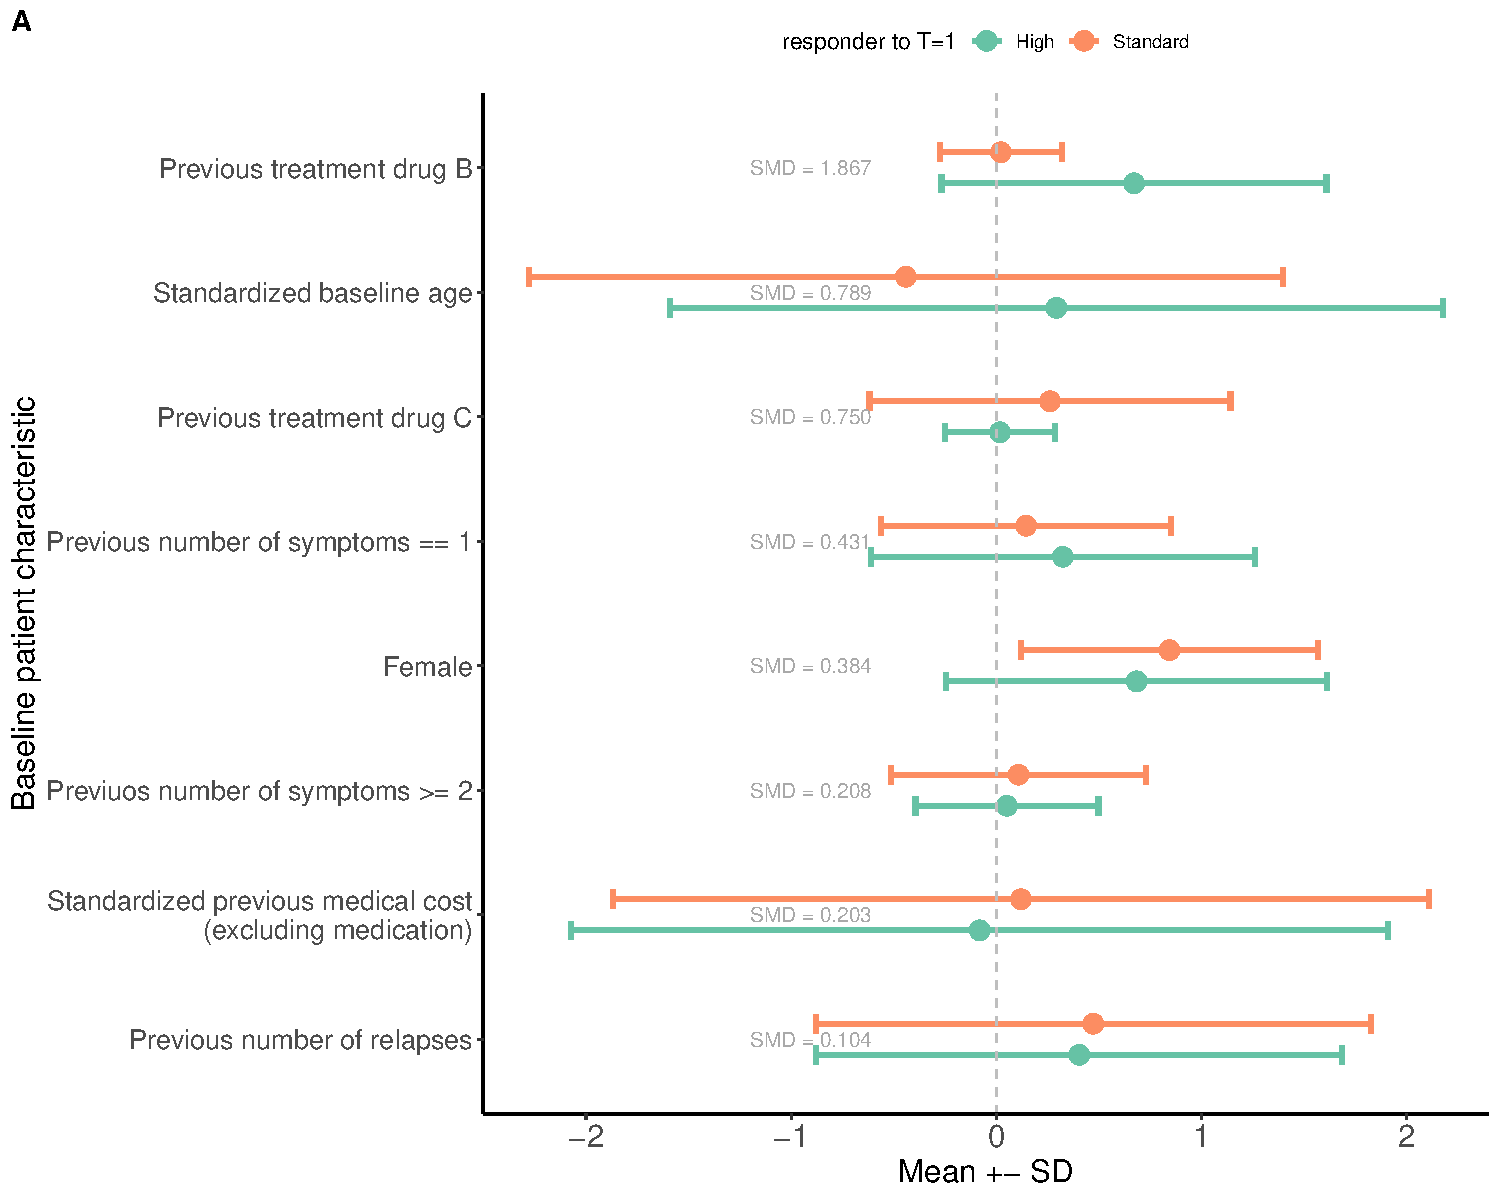
\includegraphics{chapter_18_files/figure-pdf/unicomp.visual-1.pdf}

}

\end{figure}

We can also show the density of ITR scores obtained from the score-based
methods. The results can be found in \texttt{modpm} and we used
histogram to visualize (Figure 6B).

\begin{Shaded}
\begin{Highlighting}[]
\DocumentationTok{\#\#\#\#\# Density of ITR score \#\#\#\#\#}
\NormalTok{dataplot }\OtherTok{\textless{}{-}} \FunctionTok{data.frame}\NormalTok{(}\AttributeTok{score =} \FunctionTok{factor}\NormalTok{(}\FunctionTok{rep}\NormalTok{(}\FunctionTok{c}\NormalTok{(}\StringTok{"Naive Poisson"}\NormalTok{, }\StringTok{"Contrast Regression"}\NormalTok{),}
                                          \AttributeTok{each =} \FunctionTok{length}\NormalTok{(modpm}\SpecialCharTok{$}\NormalTok{score.poisson))),}
                       \AttributeTok{value =} \FunctionTok{c}\NormalTok{(modpm}\SpecialCharTok{$}\NormalTok{score.poisson, modpm}\SpecialCharTok{$}\NormalTok{score.contrastReg))}

\NormalTok{p6b }\OtherTok{\textless{}{-}}\NormalTok{ dataplot }\SpecialCharTok{\%\textgreater{}\%}
  \FunctionTok{ggplot}\NormalTok{(}\FunctionTok{aes}\NormalTok{(}\AttributeTok{x =}\NormalTok{ value, }\AttributeTok{fill =}\NormalTok{ score)) }\SpecialCharTok{+}
  \FunctionTok{geom\_density}\NormalTok{(}\AttributeTok{alpha =} \FloatTok{0.5}\NormalTok{) }\SpecialCharTok{+}
  \FunctionTok{scale\_fill\_manual}\NormalTok{(}\AttributeTok{values =} \FunctionTok{c}\NormalTok{(}\StringTok{"dodgerblue"}\NormalTok{, }\StringTok{"gray30"}\NormalTok{)) }\SpecialCharTok{+}
  \FunctionTok{geom\_vline}\NormalTok{(}\AttributeTok{xintercept =} \DecValTok{0}\NormalTok{, }\AttributeTok{color =} \StringTok{"darkgray"}\NormalTok{, }\AttributeTok{linetype =} \StringTok{"dashed"}\NormalTok{, }\AttributeTok{size =} \DecValTok{1}\NormalTok{) }\SpecialCharTok{+}
  \FunctionTok{labs}\NormalTok{(}\AttributeTok{x =} \StringTok{"Estimated CATE score"}\NormalTok{, }\AttributeTok{y =} \StringTok{"Density"}\NormalTok{, }\AttributeTok{fill =} \StringTok{"Method"}\NormalTok{) }\SpecialCharTok{+}
  \FunctionTok{theme\_classic}\NormalTok{() }\SpecialCharTok{+}
  \FunctionTok{theme}\NormalTok{(}\AttributeTok{legend.position =} \FunctionTok{c}\NormalTok{(}\FloatTok{0.2}\NormalTok{, }\FloatTok{0.8}\NormalTok{),}
        \AttributeTok{axis.text =} \FunctionTok{element\_text}\NormalTok{(}\AttributeTok{size =} \DecValTok{13}\NormalTok{),}
        \AttributeTok{axis.title.y =} \FunctionTok{element\_text}\NormalTok{(}\AttributeTok{size =} \DecValTok{15}\NormalTok{),}
        \AttributeTok{axis.title.x =} \FunctionTok{element\_text}\NormalTok{(}\AttributeTok{size =} \DecValTok{15}\NormalTok{),}
        \AttributeTok{axis.text.x =} \FunctionTok{element\_text}\NormalTok{(}\AttributeTok{size =} \DecValTok{15}\NormalTok{),}
        \AttributeTok{strip.text.x =} \FunctionTok{element\_text}\NormalTok{(}\AttributeTok{size =} \DecValTok{12}\NormalTok{))}
\end{Highlighting}
\end{Shaded}

The ITR scores are essentially a linear combination of the baseline
characteristics, thus it might be also of interest for one to know the
corresponding coefficients (or weights) which shows how much each
baseline variable contributed to the ITR score. To make it comparable
across different scales of the baseline variables, we used the scaled
data and the model result \texttt{modpm.s} was used to extract the
coefficients and visualize as a bar plot. The coefficients can be
presented in a table as well.

\begin{Shaded}
\begin{Highlighting}[]
\CommentTok{\# Coefficients}
\NormalTok{coef }\OtherTok{\textless{}{-}}\NormalTok{ modpm.s}\SpecialCharTok{$}\NormalTok{coefficients}

\NormalTok{p6c }\OtherTok{\textless{}{-}}\NormalTok{ coef }\SpecialCharTok{\%\textgreater{}\%}
  \FunctionTok{as\_tibble}\NormalTok{(}\AttributeTok{rownames =} \StringTok{"varname"}\NormalTok{) }\SpecialCharTok{\%\textgreater{}\%}
  \FunctionTok{melt}\NormalTok{(}\AttributeTok{id.vars =} \StringTok{"varname"}\NormalTok{) }\SpecialCharTok{\%\textgreater{}\%}
  \FunctionTok{filter}\NormalTok{(variable }\SpecialCharTok{==} \StringTok{"poisson"}\NormalTok{, varname }\SpecialCharTok{!=} \StringTok{"(Intercept)"}\NormalTok{) }\SpecialCharTok{\%\textgreater{}\%}
  \FunctionTok{mutate}\NormalTok{(}\AttributeTok{absval =} \FunctionTok{abs}\NormalTok{(value),}
         \AttributeTok{sign =} \FunctionTok{ifelse}\NormalTok{(value }\SpecialCharTok{\textgreater{}} \DecValTok{0}\NormalTok{, }\StringTok{"+"}\NormalTok{, }\StringTok{"{-}"}\NormalTok{)) }\SpecialCharTok{\%\textgreater{}\%}
  \FunctionTok{arrange}\NormalTok{(absval) }\SpecialCharTok{\%\textgreater{}\%}
  \FunctionTok{mutate}\NormalTok{(}\AttributeTok{varname =} \FunctionTok{factor}\NormalTok{(varname, }\AttributeTok{levels =} \FunctionTok{unique}\NormalTok{(varname))) }\SpecialCharTok{\%\textgreater{}\%}
  \FunctionTok{ggplot}\NormalTok{(}\FunctionTok{aes}\NormalTok{(}\AttributeTok{x =}\NormalTok{ varname, }\AttributeTok{y =}\NormalTok{ absval, }\AttributeTok{fill =}\NormalTok{ sign)) }\SpecialCharTok{+}
  \FunctionTok{geom\_bar}\NormalTok{(}\AttributeTok{stat =} \StringTok{"identity"}\NormalTok{, }\AttributeTok{width =} \FloatTok{0.5}\NormalTok{) }\SpecialCharTok{+}
  \FunctionTok{scale\_fill\_brewer}\NormalTok{(}\AttributeTok{palette =} \StringTok{"Set1"}\NormalTok{) }\SpecialCharTok{+}
  \FunctionTok{scale\_x\_discrete}\NormalTok{(}\AttributeTok{labels =}\NormalTok{ labs) }\SpecialCharTok{+}
  \FunctionTok{coord\_flip}\NormalTok{() }\SpecialCharTok{+}
  \FunctionTok{labs}\NormalTok{(}\AttributeTok{y =} \StringTok{"Absolute value of the estimated coefficient of CATE scores}\SpecialCharTok{\textbackslash{}n}\StringTok{based on Poisson regression"}\NormalTok{, }\AttributeTok{x =} \StringTok{"Baseline patient characteristic"}\NormalTok{) }\SpecialCharTok{+}
  \FunctionTok{theme\_minimal}\NormalTok{() }\SpecialCharTok{+}
  \FunctionTok{theme}\NormalTok{(}\AttributeTok{legend.position =} \FunctionTok{c}\NormalTok{(}\FloatTok{0.8}\NormalTok{, }\FloatTok{0.2}\NormalTok{),}
        \AttributeTok{axis.text =} \FunctionTok{element\_text}\NormalTok{(}\AttributeTok{size =} \DecValTok{13}\NormalTok{),}
        \AttributeTok{axis.title.y =} \FunctionTok{element\_text}\NormalTok{(}\AttributeTok{size =} \DecValTok{15}\NormalTok{),}
        \AttributeTok{axis.title.x =} \FunctionTok{element\_text}\NormalTok{(}\AttributeTok{size =} \DecValTok{15}\NormalTok{),}
        \AttributeTok{axis.text.x =} \FunctionTok{element\_text}\NormalTok{(}\AttributeTok{size =} \DecValTok{15}\NormalTok{),}
        \AttributeTok{strip.text.x =} \FunctionTok{element\_text}\NormalTok{(}\AttributeTok{size =} \DecValTok{12}\NormalTok{))}

\CommentTok{\# Figure 6B, 6C}
\FunctionTok{ggarrange}\NormalTok{(p6b, p6c, }\AttributeTok{nrow =} \DecValTok{2}\NormalTok{, }\AttributeTok{labels =} \FunctionTok{c}\NormalTok{(}\StringTok{"B"}\NormalTok{, }\StringTok{"C"}\NormalTok{))}
\end{Highlighting}
\end{Shaded}

\begin{figure}[H]

{\centering 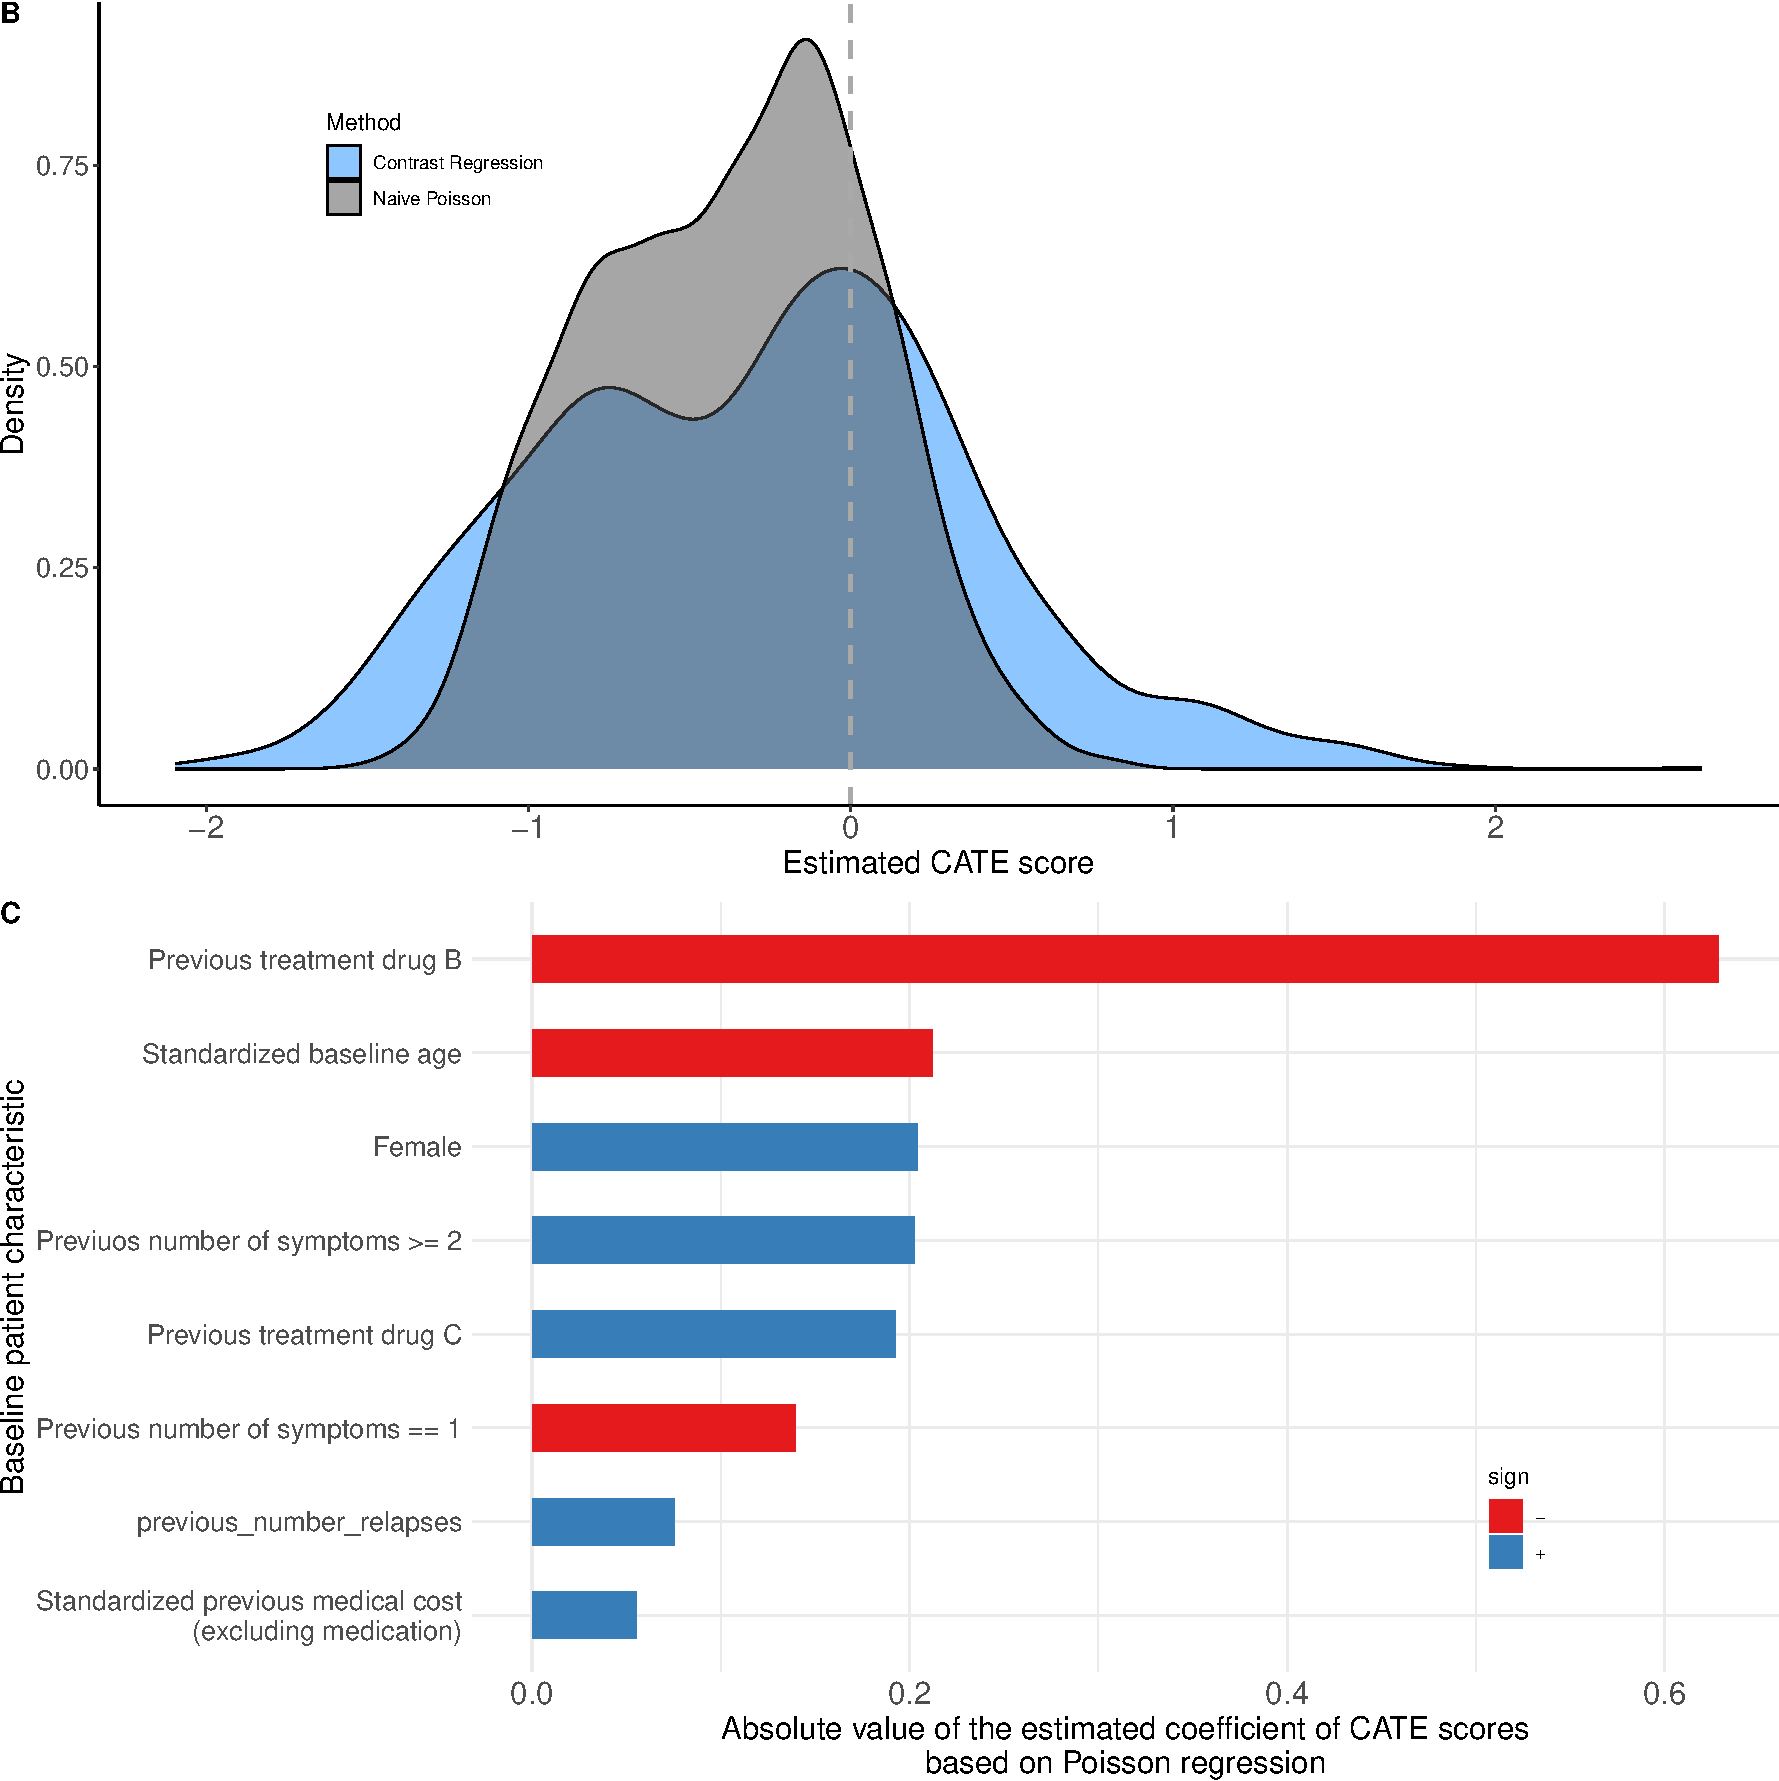
\includegraphics{chapter_18_files/figure-pdf/coefs-1.pdf}

}

\end{figure}

\begin{Shaded}
\begin{Highlighting}[]
\CommentTok{\# Coefficients presented as a table}
\NormalTok{coef }\SpecialCharTok{\%\textgreater{}\%} \FunctionTok{round}\NormalTok{(}\DecValTok{2}\NormalTok{) }\SpecialCharTok{\%\textgreater{}\%} \FunctionTok{kable}\NormalTok{() }\SpecialCharTok{\%\textgreater{}\%} \FunctionTok{kable\_styling}\NormalTok{(}\AttributeTok{full\_width =}\NormalTok{ F)}
\end{Highlighting}
\end{Shaded}

\begin{table}
\centering
\begin{tabular}{l|r|r|r}
\hline
  & poisson & contrastReg & SE\_contrastReg\\
\hline
(Intercept) & -0.30 & -0.25 & 0.46\\
\hline
age.z & -0.21 & -0.23 & 0.17\\
\hline
female & 0.20 & 0.29 & 0.43\\
\hline
prevtrtB & -0.63 & -0.86 & 0.36\\
\hline
prevtrtC & 0.19 & 0.21 & 0.54\\
\hline
prevnumsymp1 & -0.14 & -0.42 & 0.39\\
\hline
prevnumsymp2p & 0.20 & 1.05 & 0.58\\
\hline
previous\_cost.z & 0.06 & 0.13 & 0.18\\
\hline
previous\_number\_relapses & 0.08 & 0.26 & 0.23\\
\hline
\end{tabular}
\end{table}

\hypertarget{version-info-7}{%
\section*{Version info}\label{version-info-7}}
\addcontentsline{toc}{section}{Version info}

\markright{Version info}

This chapter was rendered using the following version of R and its
packages:

\begin{verbatim}
R version 4.2.3 (2023-03-15 ucrt)
Platform: x86_64-w64-mingw32/x64 (64-bit)
Running under: Windows 10 x64 (build 19045)

Matrix products: default

locale:
[1] LC_COLLATE=Dutch_Netherlands.utf8  LC_CTYPE=Dutch_Netherlands.utf8   
[3] LC_MONETARY=Dutch_Netherlands.utf8 LC_NUMERIC=C                      
[5] LC_TIME=Dutch_Netherlands.utf8    

attached base packages:
[1] stats     graphics  grDevices utils     datasets  methods   base     

other attached packages:
 [1] fastDummies_1.6.3 reshape2_1.4.4    truncnorm_1.0-9   table1_1.4.3     
 [5] kableExtra_1.3.4  knitr_1.43        ggpubr_0.6.0      MASS_7.3-60      
 [9] corrplot_0.92     caret_6.0-94      lattice_0.21-8    gbm_2.1.8.1      
[13] tableone_0.13.2   rpart.plot_3.1.1  rpart_4.1.19      precmed_1.0.0    
[17] DTRreg_1.7        magrittr_2.0.3    lubridate_1.9.2   forcats_1.0.0    
[21] stringr_1.5.0     dplyr_1.1.2       purrr_1.0.1       readr_2.1.4      
[25] tidyr_1.3.0       tibble_3.2.1      ggplot2_3.4.2     tidyverse_2.0.0  

loaded via a namespace (and not attached):
  [1] colorspace_2.1-0      ggsignif_0.6.4        class_7.3-22         
  [4] ggridges_0.5.4        htmlTable_2.4.1       ggstance_0.3.6       
  [7] base64enc_0.1-3       proxy_0.4-27          rstudioapi_0.14      
 [10] listenv_0.9.0         farver_2.1.1          prodlim_2023.03.31   
 [13] fansi_1.0.4           xml2_1.3.4            codetools_0.2-19     
 [16] splines_4.2.3         polyclip_1.10-4       Formula_1.2-5        
 [19] jsonlite_1.8.5        pROC_1.18.2           broom_1.0.5          
 [22] cluster_2.1.4         geepack_1.3.9         ggforce_0.4.1        
 [25] data.tree_1.0.0       httr_1.4.6            DiagrammeR_1.0.10    
 [28] compiler_4.2.3        randomForestSRC_3.2.2 backports_1.4.1      
 [31] Matrix_1.5-4.1        fastmap_1.1.1         survey_4.2-1         
 [34] cli_3.6.1             tweenr_2.0.2          visNetwork_2.1.2     
 [37] htmltools_0.5.5       tools_4.2.3           gtable_0.3.3         
 [40] glue_1.6.2            MESS_0.5.9            Rcpp_1.0.10          
 [43] carData_3.0-5         vctrs_0.6.3           svglite_2.1.1        
 [46] nlme_3.1-162          iterators_1.0.14      timeDate_4022.108    
 [49] gower_1.0.1           xfun_0.39             globals_0.16.2       
 [52] rvest_1.0.3           timechange_0.2.0      lifecycle_1.0.3      
 [55] geeM_0.10.1           mosaicCore_0.9.2.1    rstatix_0.7.2        
 [58] future_1.32.0         scales_1.2.1          ipred_0.9-14         
 [61] hms_1.1.3             parallel_4.2.3        RColorBrewer_1.1-3   
 [64] yaml_2.3.7            gridExtra_2.3         labelled_2.11.0      
 [67] gam_1.22-2            stringi_1.7.12        foreach_1.5.2        
 [70] checkmate_2.2.0       e1071_1.7-13          hardhat_1.3.0        
 [73] lava_1.7.2.1          shape_1.4.6           systemfonts_1.0.4    
 [76] rlang_1.1.1           pkgconfig_2.0.3       evaluate_0.21        
 [79] labeling_0.4.2        recipes_1.0.6         htmlwidgets_1.6.2    
 [82] cowplot_1.1.1         tidyselect_1.2.0      parallelly_1.36.0    
 [85] ggformula_0.10.4      plyr_1.8.8            R6_2.5.1             
 [88] Hmisc_5.1-0           generics_0.1.3        DBI_1.1.3            
 [91] foreign_0.8-84        pillar_1.9.0          haven_2.5.2          
 [94] withr_2.5.0           abind_1.4-5           survival_3.5-5       
 [97] nnet_7.3-19           future.apply_1.11.0   car_3.1-2            
[100] utf8_1.2.3            tzdb_0.4.0            rmarkdown_2.22       
[103] grid_4.2.3            data.table_1.14.8     ModelMetrics_1.2.2.2 
[106] webshot_0.5.4         digest_0.6.31         stats4_4.2.3         
[109] munsell_0.5.0         glmnet_4.1-7          viridisLite_0.4.2    
[112] mitools_2.4          
\end{verbatim}

\hypertarget{references-4}{%
\section*{References}\label{references-4}}
\addcontentsline{toc}{section}{References}

\markright{References}

\hypertarget{refs}{}
\begin{CSLReferences}{1}{0}
\leavevmode\vadjust pre{\hypertarget{ref-Baker_2009}{}}%
Baker, William L, Erica L Baker, and Craig I Coleman. 2009.
{``Pharmacologic Treatments for Chronic Obstructive Pulmonary Disease: A
Mixed-Treatment Comparison Meta-Analysis.''} \emph{Pharmacotherapy} 29
(8): 891--905. \url{https://doi.org/10.1592/phco.29.8.891}.

\leavevmode\vadjust pre{\hypertarget{ref-coulombe_weighted_2021}{}}%
Coulombe, Janie, Erica E. M. Moodie, and Robert W. Platt. 2020.
{``Weighted Regression Analysis to Correct for Informative Monitoring
Times and Confounders in Longitudinal Studies.''} \emph{Biometrics} 77
(1): 162--74. \url{https://doi.org/10.1111/biom.13285}.

\leavevmode\vadjust pre{\hypertarget{ref-Coulombe_2022}{}}%
Coulombe, Janie, Erica E. M. Moodie, Robert W. Platt, and Christel
Renoux. 2022. {``Estimation of the Marginal Effect of Antidepressants on
Body Mass Index Under Confounding and Endogenous Covariate-Driven
Monitoring Times.''} \emph{The Annals of Applied Statistics} 16 (3).
\url{https://doi.org/10.1214/21-aoas1570}.

\leavevmode\vadjust pre{\hypertarget{ref-debray_methods_2023}{}}%
Debray, Thomas PA, Gabrielle Simoneau, Massimiliano Copetti, Robert W
Platt, Changyu Shen, Fabio Pellegrini, and Carl de Moor. 2023.
{``Methods for Comparative Effectiveness Based on Time to Confirmed
Disability Progression with Irregular Observations in Multiple
Sclerosis.''} \emph{Statistical Methods in Medical Research}, June,
096228022311720. \url{https://doi.org/10.1177/09622802231172032}.

\leavevmode\vadjust pre{\hypertarget{ref-panaccione_efficacy_2023}{}}%
Panaccione, Remo, Eric B Collins, Gil Y Melmed, Severine Vermeire,
Silvio Danese, Peter D R Higgins, Christina S Kwon, et al. 2023.
{``Efficacy and Safety of Advanced Therapies for Moderately to Severely
Active Ulcerative Colitis at Induction and Maintenance: An Indirect
Treatment Comparison Using Bayesian Network Meta-Analysis.''}
\emph{Crohn's \& Colitis 360} 5 (2).
\url{https://doi.org/10.1093/crocol/otad009}.

\leavevmode\vadjust pre{\hypertarget{ref-selvarajan_efficacy_2022}{}}%
Selvarajan, Sandhiya, Annuja Anandaradje, Santhosh Shivabasappa, Deepthy
Melepurakkal Sadanandan, N. Sreekumaran Nair, and Melvin George. 2022.
{``Efficacy of Pharmacological Interventions in {COVID}-19: A Network
Meta-Analysis.''} \emph{British Journal of Clinical Pharmacology} 88
(9): 4080--91. \url{https://doi.org/10.1111/bcp.15338}.

\leavevmode\vadjust pre{\hypertarget{ref-Siemieniuk_2020}{}}%
Siemieniuk, Reed AC, Jessica J Bartoszko, Dena Zeraatkar, Elena Kum,
Anila Qasim, Juan Pablo Dı́az Martinez, Ariel Izcovich, et al. 2020.
{``Drug Treatments for Covid-19: Living Systematic Review and Network
Meta-Analysis.''} \emph{{BMJ}}, July, m2980.
\url{https://doi.org/10.1136/bmj.m2980}.

\leavevmode\vadjust pre{\hypertarget{ref-yadlowsky_estimation_2021}{}}%
Yadlowsky, Steve, Fabio Pellegrini, Federica Lionetto, Stefan Braune,
and Lu Tian. 2020. {``Estimation and Validation of Ratio-Based
Conditional Average Treatment Effects Using Observational Data.''}
\emph{Journal of the American Statistical Association} 116 (533):
335--52. \url{https://doi.org/10.1080/01621459.2020.1772080}.

\leavevmode\vadjust pre{\hypertarget{ref-zhao_effectively_2013}{}}%
Zhao, Lihui, Lu Tian, Tianxi Cai, Brian Claggett, and L. J. Wei. 2013.
{``Effectively Selecting a Target Population for a Future Comparative
Study.''} \emph{Journal of the American Statistical Association} 108
(502): 527--39. \url{https://doi.org/10.1080/01621459.2013.770705}.

\end{CSLReferences}



\end{document}
